\documentclass[12pt,a4paper]{report}

%%
% to enumerate subsubsection
%%
\addtocounter{tocdepth}{3}
\setcounter{secnumdepth}{3}
% \usepackage{tgtermes}
% \usepackage{pgfplots}
% \usepgfplotslibrary{external} 
% \tikzexternalize
\usepackage{parskip}
\usepackage{setspace}
\usepackage[a4paper, margin=0.984252in]{geometry}
\usepackage[T1]{fontenc}
\usepackage[breaklinks,hidelinks]{hyperref}
\usepackage[utf8]{inputenc}
\usepackage{graphicx} 
\usepackage{color,soul}
\usepackage{tikz}
\usepackage{amsmath, amssymb}
% \usepackage{indentfirst}
% \usepackage{cite}
\usepackage{natbib}
\usepackage[nameinlink,noabbrev]{cleveref}
\usepackage[capposition=top]{floatrow}
\usepackage{float}
% \usepackage[tableposition=top]{caption}
% \floatsetup[table]{capposition=top}
\usepackage{caption}
\usepackage{xfrac}
\usepackage{braket}
\usepackage[toc,page]{appendix}
\usepackage{longtable}
\usepackage{tabularx}
\usepackage{adjustbox}
\usepackage{multirow}
\usepackage{arydshln}
\usepackage{pdfpages}
% \usepackage{scrextend} % add margin
% \usepackage{hyperref}
% \usepackage{physics}
\def\changemargin#1#2{\list{}{\rightmargin#2\leftmargin#1}\item[]}
\let\endchangemargin=\endlist 

%%
% to enumerate subsubsection
%%
\addtocounter{tocdepth}{3}
\setcounter{secnumdepth}{3}
\renewcommand{\baselinestretch}{1.3}
% \linespread{1.5}
% \setlength{\parindent}{0em}
% \setlength{\parskip}{1em}
% \usepackage{setspace}
% \setstretch{1.5}

% Snippet
\newcommand{\BSM}{Black--Scholes--Merton }
\newcommand{\lnorm}{log-normally }
\newcommand{\bmotion}{Brownian Motion }
\newcommand{\stvar}{stochastic variable }
\newcommand{\wienpro}{Wiener process }
\newcommand{\markpro}{Markov process }

% 
% Bunch of new commands
% 
% brownian motion
\newcommand{\dBm}{dW\left(t\right)}
\newcommand{\dpoiss}{dq\left(t\right)}
\newcommand{\DBm}{\delta{W\left(t\right)}}
\newcommand{\Bm}{W\left(t\right)}
\newcommand{\Bmsub}[1]{W_{#1}\left(t\right)}
\newcommand{\Dt}{\Delta t} 
\newcommand{\Bmdist}{\DBm \sim N \left( 0, \Dt \right)}
\newcommand{\ft}{f\left(t, \Bm \right)}
\newcommand{\E}{\mathop{\mathbb{E}}}
\newcommand{\ct}{c\left(t, x\right)}
\newcommand{\dcx}{\frac{\delta\ct}{\delta x}}
\newcommand{\dciix}{\frac{\delta^2\ct}{\delta x^2}}
\newcommand{\dct}{\frac{\delta\ct}{\delta t}}
\newcommand{\N}[1]{N\left(#1\right)}
\newcommand{\dsub}[1]{d_{#1}\left(\Dt, x\right)}
\newcommand{\call}[2]{c\left( #1, #2\right)}
% % about stock
\newcommand{\St}{S\left(t\right)}
\newcommand{\Vt}{V\left(t\right)}
\newcommand{\Si}{S\left(0\right)}
\newcommand{\dSt}{dS\left(t\right)}
\newcommand{\DSt}{\Delta S\left(t\right)}
\newcommand{\dSr}{\frac{\dSt}{\St}}
\newcommand{\DSr}{\frac{\DSt}{\St}}
\newcommand{\Scontinuous}{\St = \Si e^{\sigma\Bm + \left(\alpha - \frac{1}{2 \sigma^2}\right)t}}
\newcommand{\Itobmdiff}{d\ft = \left[\frac{\partial \ft }{\partial t} + \frac{1}{2} \frac{\partial ^2\ft }{\partial x^2}\right]dt + \frac{\partial \ft}{\partial x} \dBm}
\newcommand{\Scontinousdiff}{d\St &= \alpha \St dt + \sigma \St \dBm}
\newcommand{\Scontinuousrate}{\dSr &= \alpha dt + \sigma \dBm}
 \newcommand{\Sdiscretediff}{d\St &= \alpha \St \Dt + \sigma \St \dBm}
\newcommand{\Sshort}{\Si e^{X}}
\newcommand{\CCRdist}{X \sim N\left(\left(\alpha - \frac{1}{2}\sigma^2\right)t, \sigma^2 t\right)}
\newcommand{\Sdiscreterate}{\DSr &= \alpha \Delta t + \sigma \DBm}
\newcommand{\Sdiscreterateexp}{\E \DSr = \alpha \Dt}
\newcommand{\Sdiscreteratevar}{var \DSr = \sigma ^2 \Dt}
\newcommand{\Sdiscreteratedist}{\DSr \sim N\left(\alpha\Dt, \sigma\Dt\right)}
\newcommand{\Sexp}{\E\St = \Si e^{\alpha t}}
\newcommand{\Svar}{var\St = \Si^2 e^{2\alpha t}\left(e^{\sigma^2 t} - 1\right)}
\newcommand{\Sshortt}{\St = \Si e^{X t}}
\newcommand{\CCRt}{X = \frac{1}{t} \ln{\frac{\St}{\Si}}}
\newcommand{\CCRtdist}{X \sim N\left(\alpha - \frac{\sigma^2}{2}, \frac{\sigma^2}{t}\right)}
\newcommand{\BSMpde}{\dct + r x \dcx + \frac{1}{2} \sigma^2 x^2 \dciix = r\ct}
\newcommand{\BSMeq}[1]{r\call{t}{#1} = \frac{\partial \call{t}{#1}}{\partial t} + r #1 \frac{\partial \call{t}{#1}}{\partial #1} + \frac{1}{2} \sigma ^2 #1 ^2 \frac{\partial ^2 \call{t}{#1}}{\partial #1 ^2}}
\newcommand{\BSMGreeks}[1]{r\call{t}{#1} = \Theta + r #1 \Delta + \frac{1}{2} \sigma ^2 #1 ^2 \Gamma}
\newcommand{\BSMsol}{\ct &= x\N{\dsub{+}} - K e^{-r\Dt} \N{\dsub{-}}}
\newcommand{\dpm}{\dsub{\pm} &= \frac{1}{\sigma\sqrt{\Dt}} \left[\log\frac{x}{K} + \left(r \pm \frac{\sigma^2}{2}\Dt\right)\right]}

% CIR Stock price Stochastic process
\newcommand{\HSVstock}{
  d\St &= \alpha \St dt + \sqrt{\Vt} \St d \Bmsub{S}
}

% CIR Stock price Stochastic process
\newcommand{\HSVstockriskless}{
  d\St &= r \St dt + \sqrt{\Vt} \St d \Bmsub{S}
}

% CIR volatility
\newcommand{\HSVvol}{
  d\Vt &= \kappa\left(\theta - \Vt \right) dt + \sigma \sqrt{\Vt} d \Bmsub{V}
}


% CIR volatility
\newcommand{\HSVvolriskless}{
  d\Vt &= \kappa^{*} \left(\theta^{*} - \Vt \right) dt + \sigma \sqrt{\Vt} d \Bmsub{V}
}

\newcommand{\dportfolio}{dX\left(t\right) = \Delta\left(t\right) d\St + r \left(X\left(t\right) - \Delta\left(t\right) \St \right) dt}

\usepackage{Sweave}
\begin{document}

\Sconcordance{concordance:index.tex:index.Rnw:%
1 6 1}
\Sconcordance{concordance:index.tex:./preamble/usepackage.Rnw:ofs 7:%
1 21 1}
\Sconcordance{concordance:index.tex:./preamble/misc.Rnw:ofs 29:%
1 6 1}
\Sconcordance{concordance:index.tex:./preamble/snippet.Rnw:ofs 36:%
1 7 1}
\Sconcordance{concordance:index.tex:./preamble/formula.Rnw:ofs 44:%
1 71 1}
\Sconcordance{concordance:index.tex:index.Rnw:ofs 116:%
12 1 1 1 0 24 1}
\Sconcordance{concordance:index.tex:./methodology.Rnw:ofs 143:%
1 485 1}
\Sconcordance{concordance:index.tex:index.Rnw:ofs 629:%
39 12 1}


\setkeys{Gin}{width=8.3in}
\begin{titlepage}
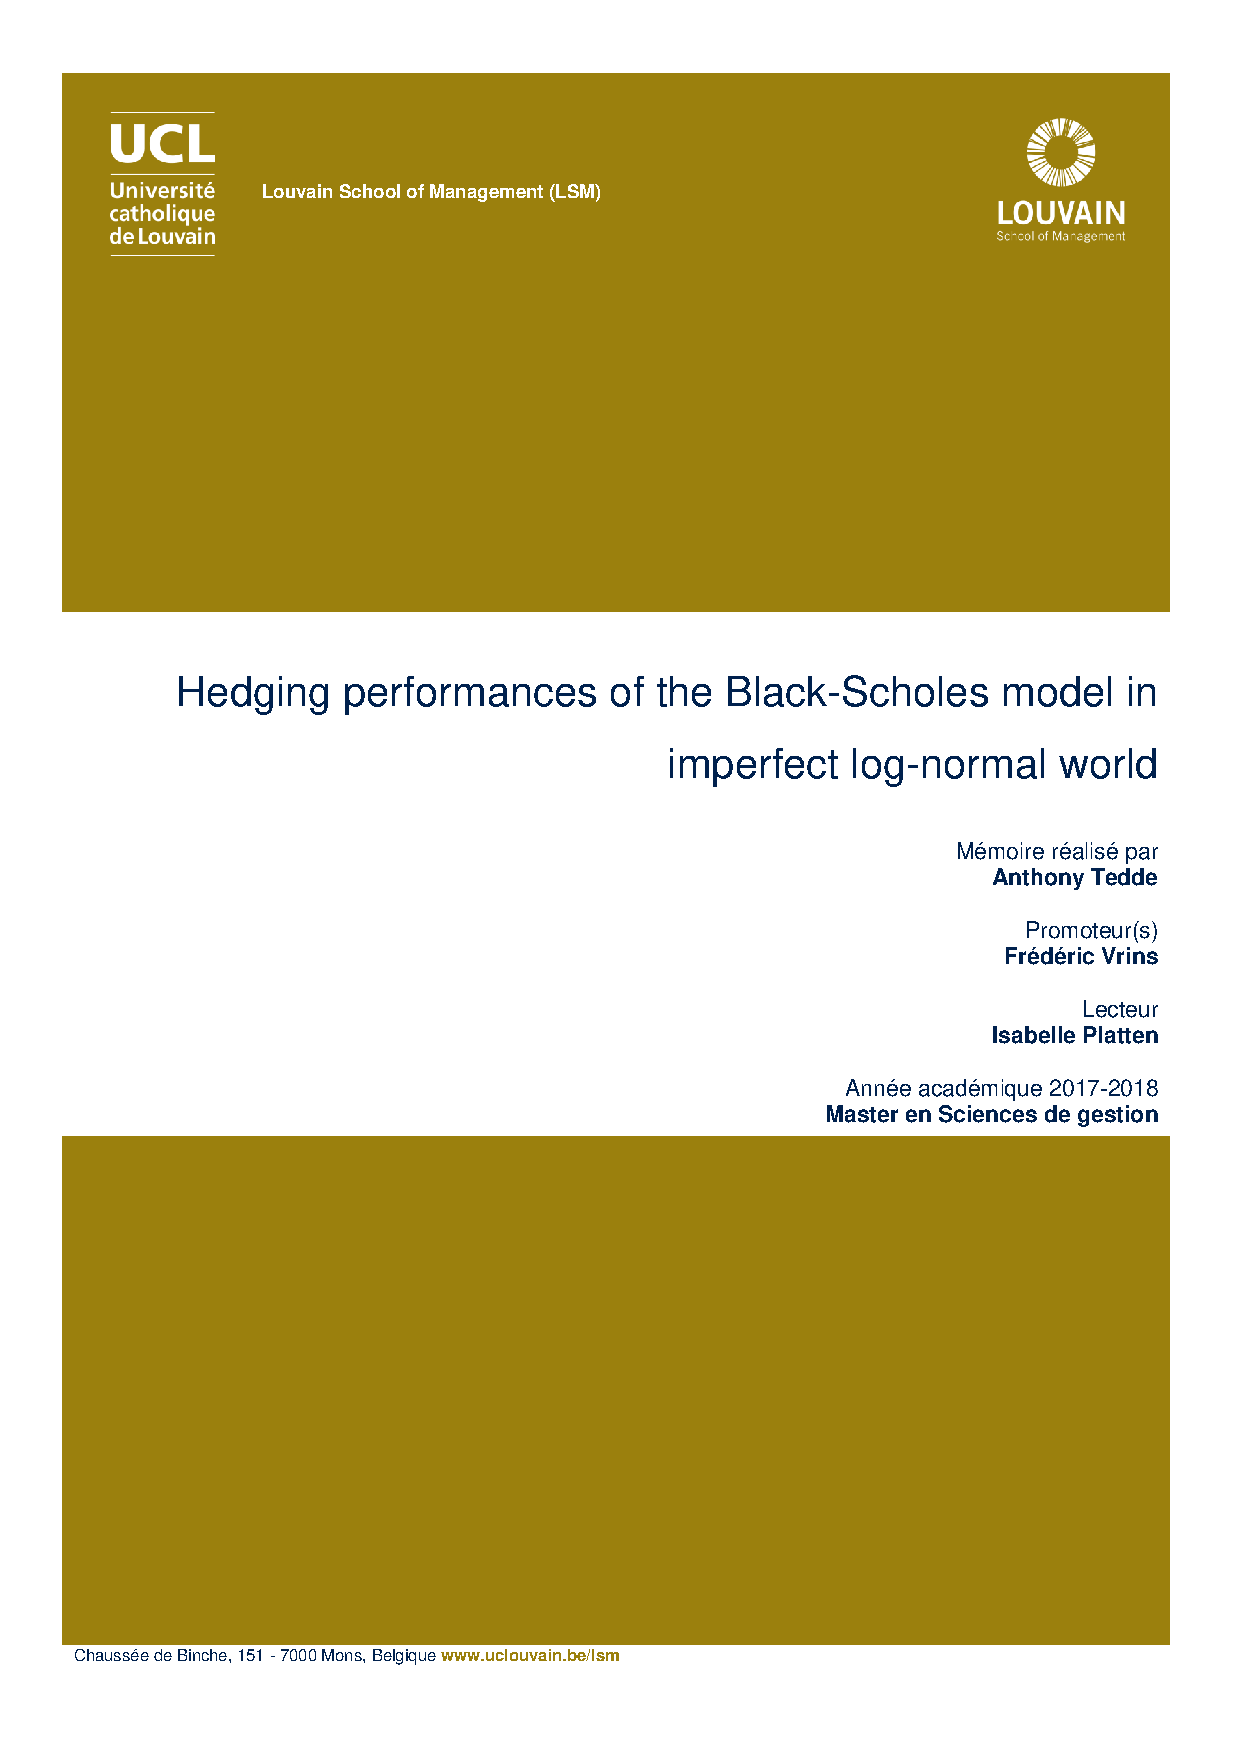
\includepdf{cover.pdf}
\end{titlepage}

\newpage\null\thispagestyle{empty}\newpage


\setkeys{Gin}{width=0.8\textwidth}



\pagenumbering{roman}
\chapter*{Abstract}
\addcontentsline{toc}{chapter}{Abstract}
 
The study developed in the current master thesis concerns the Black-Scholes-Merton (BSM) method initially intended to give a fair price to options for which a geometric Brownian motion (GBM) drives the underlying asset.
Indeed this model works remarkably well provided that the underpinned assumptions are respected with the most restrictive one stating that the distribution of the log-returns of the underlying asset has to be normal.
However, empirical results show that this constraint of log-normality does not hold for real-life trials and consequently break the more key hypothesis of the aforementioned model.

The primary purpose of the analysis developed in that work is to assess how wrong goes the BSM equation while the underlying asset is not a GBM.
To that end, others models will be investigated, namely, the Merton jump diffusion (MJD) and Heston stochastic volatility (HSV) models.
Each of it bears a new characteristic. The MJD brings jumps to the paths of the underlying processes whilst HSV comes with a volatility parameter that evolves with times unlike the deterministic one inherent to BSM. These specificities affect the log-returns distributions that are no more normal.

Accordingly, once calibrated, those models will be used to simulate a world where the assumption of log-normality of the BSM model does not hold anymore. The study case explored is to measure how the BSM equation will react when its central assumption is broken.
To do this, the performance of the delta-neutral portfolios of BSM, MJD and HSV processes will be benchmarked.

As a subanalysis, another goal of that master thesis is to examine if, with a unique set of parameters, the HSV and MJD models can reproduce the volatility smiles constructed from the options prices provided by the market.
A conclusion would be that those models are versatile enough to cover a broader range of market prices than the BSM model itself.
\chapter*{Acknowledgements}
\addcontentsline{toc}{chapter}{Acknowledgements}

First and foremost, I want to address all my gratitude to Anne, and our two wonderful children, Elsa and Valentin, for their patience and huge support. They gave me all the strength needed to go beyond my self-motivation.

Many thanks to all of my family and precious friends that make the life more pleasant. I especially think of Nonna Emma, Mario, Josiane, Maud, Eddy, Christelle, Sébastien, and Pierre. 

Thank you mum and dad.

Last but not least, I want to sincerely thank Pr. Frédéric Vrins for trusting me. It was a real pleasure to meet you.




{\setstretch{1.0}
\tableofcontents
\clearpage

\listoffigures
 \clearpage


\listoftables}
\clearpage



\pagenumbering{arabic}
% \SweaveInput{introduction}
% \SweaveInput{upstream}
% \SweaveInput{BSM}
%%%%%%%%%%%%%%%%%%%%%%%%%%%%%%%%%%%%%%%%%%%%%%%%%%%%%%%%%%%%%%%%%%%%%%%%%%%%%%%%
%
%  CHAPTER:Other Models to be considered
%
%%%%%%%%%%%%%%%%%%%%%%%%%%%%%%%%%%%%%%%%%%%%%%%%%%%%%%%%%%%%%%%%%%%%%%%%%%%%%%%%
\chapter{Other Models to be considered}
\label{cha:OtherModel}

In this chapter are explored models that will substitute the geometric Brownian motion for the stock prices evolution along with the related option pricing method.

The first considered model is the Merton jump-diffusion (MJD) that brings jump to the course of a stochastic process while the second is the Heston stochastic volatility model that allows the volatility parameter to evolve through time.

At the end of that chapter, a method developed by \citet{heston1993} illustrates how to compute the prices of options based on such underlying by using their characteristic function.




%%%%%%%%%%%%%%%%%%%%%%%%%%%%%%%%%%%%%%%%%%%%%%%%
% SUBSECTION: Mixed jump-diffusionModel
%%%%%%%%%%%%%%%%%%%%%%%%%%%%%%%%%%%%%%%%%%%%%%%%
\section{Merton Mixed jump-diffusion Model}
\label{sec:other:merton}

In his paper, \citet{merton76} provides a model for stock price evolution involving jumps (\cref{eq:other:merton:pde}). 


\begin{align}
  \St &= S\left(0\right) e^{\left(\alpha - \frac{\sigma^2}{2} - \lambda \kappa\right) t + \sigma \Bm + \sum_{i=1}^{N_t} Y_i}
  \label{eq:other:merton:pde}
\end{align}
  
According to \citet{merton76}, there are two specific sources of uncertainty explained by the model (\cref{eq:other:merton:pde}). 

The first one is qualified as normal, repeatedly arising with low effects and keeping the stock price motion continuous from time to time. These small changes on the price are modeled by a Wiener process, such as it was the case in equation \ref{eq:underlying:geometric:closed}. The cause of these fluctuations is explained by a temporary unbalanced between the supply and demand \citet{merton76}.

Another type of changes, occurring during the stock lifecycle, is qualified as abnormal by \citet{merton76}. 
Such "abnormalities" happen less frequently, are unpredictable in their frequency and produce bigger effects on the stock price by giving rise to jumps during the course of the stock path, and therefore breaking its continuity. The jump process is constructed on a double basis. 

Firstly, the occurrence (i.e. the number of jumps arising throughout a given period of time) is computed thanks to a Poisson-driven process according to a parameter $\lambda$. 
$\lambda$ denotes the number of jumps per unit of time. Consequently, the probability that a jump occurs during a time range of $\Delta t$ is equal to $\lambda dt$ (event $A$, eq. \ref{eq:PA}), whereas the probability that there are no jump during the same range of time is $1 - \lambda dt$, (event $B$, eq. \ref{eq:PB}) (\citet{matsuda2004}). While event C, from \cref{eq:PC}, refers to the event that more than one jump occurs during the same small delta time.

\begin{align}
  \mathop{\mathbb{P}} \{A\}&\cong \lambda dt  \label{eq:PA}\\
  \mathop{\mathbb{P}} \{B\}&\cong 1 - \lambda dt  \label{eq:PB}\\
  \mathop{\mathbb{P}} \{C\}&\cong   0 \label{eq:PC}
\end{align}

On the other hand, after the occurrence, the size of the jump matters. Such as the frequency, a statistic law characterizes the importance of the jump. Following \citet{merton76}, the log-normal law is used. \citet{matsuda2004} offers the \crefrange{eq:yt}{eq:lny} to summarize the law and the parameters that describe the jump intensity.
 
\begin{align}
  y_t  &\sim lognormal( e^{\mu + \frac{1}{2} \delta^2}, 
                        e^{2 \mu + \delta ^2} (e^{\delta^2} - 1)) 
  \label{eq:yt} \\
  y_t - 1 &\sim lognormal( \kappa \equiv e^{\mu + \frac{1}{2} \delta^2} - 1, 
                        e^{2 \mu + \delta ^2} (e^{\delta^2} - 1)) 
  \label{eq:ytminus1} \\
  \ln{y_t} &\sim normal(\mu, \delta^ 2)
  \label{eq:lny}
\end{align}
with $y_t$, $y_t - 1$ and $\ln{y_t} \equiv Y_t$ standing respectively for "absolute price jump size", "relative price jump size" and "log price jump size" (\citet{matsuda2004}).

 
The Merton's jump-diffusion process is be able to capture positive / negative skewness (see \cref{sub:MertonSkewness}) and excess kurtosis (see \cref{sub:MertonKurtosis}) of the log-return density function, in accordance with \citet{merton76}. 


%%%%%%%%%%%%%%%%%%%%%%%%%%%%%%%%%%%%%%%%%%%%%%%%
% SUBSECTION: Risk-neutralized process
%%%%%%%%%%%%%%%%%%%%%%%%%%%%%%%%%%%%%%%%%%%%%%%%
\subsection{Risk-neutralized process}
\label{sub:other:merton:risk}

In order to find the fair price of an option depending on an underlying that follows such a jump-diffusion process, \citet{merton76} turns \cref{eq:other:merton:pde} into one risk-neutral.

\begin{align}
  \St &= S\left(0\right) e^{\left(r - \frac{\sigma^2}{2} - \lambda \kappa\right) t + \sigma \Bm + \sum_{i=1}^{N_t} Y_i}
  \label{eq:other:merton:pde:riskneutral}
\end{align}

\citet{merton76} argues in his paper that the jump component of \cref{eq:other:merton:pde} can be diversified in a well-balanced portfolio and consequently does not need to be risk-neutralized.

However, likewise it was done by \citet{bs}, the drift part of \cref{eq:other:merton:pde} is risk-neutralized by turning the rate $\alpha$ into its riskfree counterpart $r$, as shown by \cref{eq:other:merton:pde:riskneutral}.



%%%%%%%%%%%%%%%%%%%%%%%%%%%%%%%%%%%%%%%%%%%%%%%%
% SUBSECTION: Graphical representation
%%%%%%%%%%%%%%%%%%%%%%%%%%%%%%%%%%%%%%%%%%%%%%%%
\subsection{Graphical representation}
\label{sub:other:merton:graphical}   

\Cref{p:other:merton:path} shows a unique time-series generated using an implementation of \cref{eq:other:merton:pde}. A jump is clearly marked at day 363. While
\cref{t:other:merton:path}, which is a subset of the time-series drawn in \cref{p:other:merton:path}, illustrates numerically when the jump occurs.

\begin{table}[ht]
\centering
\begin{tabular}{ll}
  \hline
 time periods (days)& stock price\\ 
  \hline
  0   &50.00 \\ 
  1   &49.72 \\ 
  2   &49.87 \\ 
  \vdots & \vdots \\
  323 &83.44 \\ 
  324 &94.98 \\ 
  \vdots & \vdots \\
  363 &97.41 \\ 
  364 &97.07 \\ 
  365 &97.00 \\ 
   \hline
\end{tabular}
\caption{Merton Mixed jump-diffusion time-series}
\label{t:other:merton:path}
\end{table}

\begin{figure}[ht]
  \centering
  % Created by tikzDevice version 0.11 on 2018-07-12 22:38:50
% !TEX encoding = UTF-8 Unicode
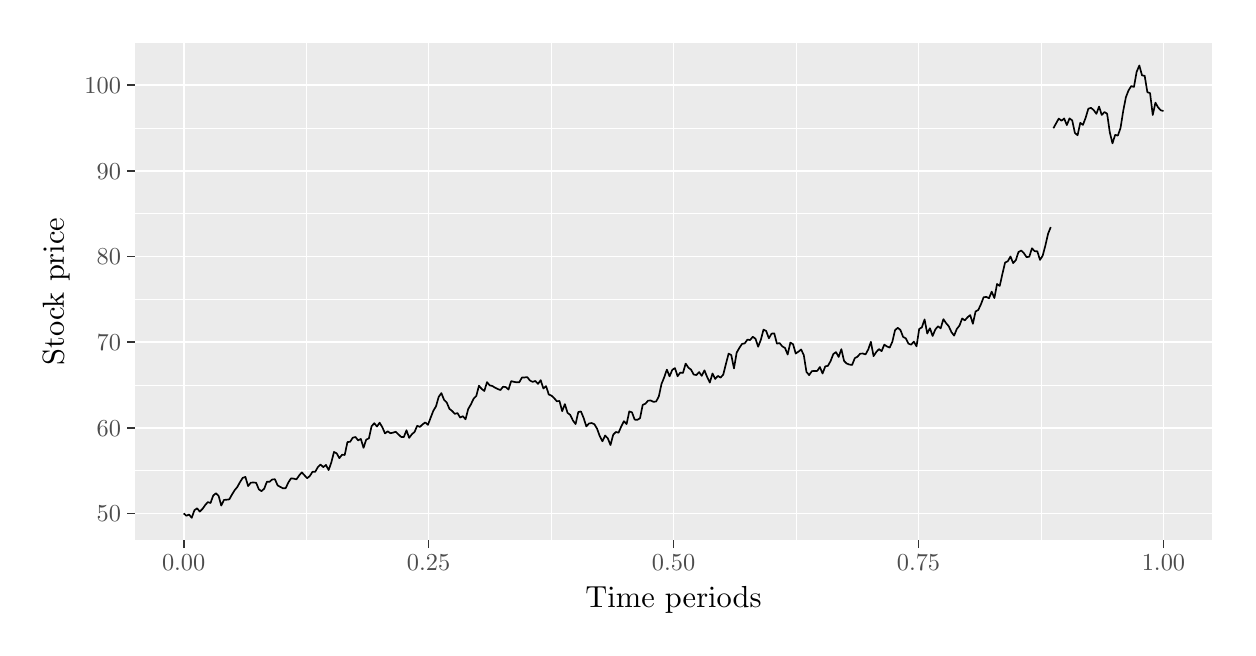
\begin{tikzpicture}[x=1pt,y=1pt]
\definecolor{fillColor}{RGB}{255,255,255}
\path[use as bounding box,fill=fillColor,fill opacity=0.00] (0,0) rectangle (433.62,216.81);
\begin{scope}
\path[clip] (  0.00,  0.00) rectangle (433.62,216.81);
\definecolor{drawColor}{RGB}{255,255,255}
\definecolor{fillColor}{RGB}{255,255,255}

\path[draw=drawColor,line width= 0.6pt,line join=round,line cap=round,fill=fillColor] (  0.00,  0.00) rectangle (433.62,216.81);
\end{scope}
\begin{scope}
\path[clip] ( 38.67, 31.53) rectangle (428.12,211.31);
\definecolor{fillColor}{gray}{0.92}

\path[fill=fillColor] ( 38.67, 31.53) rectangle (428.12,211.31);
\definecolor{drawColor}{RGB}{255,255,255}

\path[draw=drawColor,line width= 0.3pt,line join=round] ( 38.67, 56.77) --
	(428.12, 56.77);

\path[draw=drawColor,line width= 0.3pt,line join=round] ( 38.67, 87.71) --
	(428.12, 87.71);

\path[draw=drawColor,line width= 0.3pt,line join=round] ( 38.67,118.64) --
	(428.12,118.64);

\path[draw=drawColor,line width= 0.3pt,line join=round] ( 38.67,149.58) --
	(428.12,149.58);

\path[draw=drawColor,line width= 0.3pt,line join=round] ( 38.67,180.52) --
	(428.12,180.52);

\path[draw=drawColor,line width= 0.3pt,line join=round] (100.63, 31.53) --
	(100.63,211.31);

\path[draw=drawColor,line width= 0.3pt,line join=round] (189.14, 31.53) --
	(189.14,211.31);

\path[draw=drawColor,line width= 0.3pt,line join=round] (277.65, 31.53) --
	(277.65,211.31);

\path[draw=drawColor,line width= 0.3pt,line join=round] (366.16, 31.53) --
	(366.16,211.31);

\path[draw=drawColor,line width= 0.6pt,line join=round] ( 38.67, 41.30) --
	(428.12, 41.30);

\path[draw=drawColor,line width= 0.6pt,line join=round] ( 38.67, 72.24) --
	(428.12, 72.24);

\path[draw=drawColor,line width= 0.6pt,line join=round] ( 38.67,103.17) --
	(428.12,103.17);

\path[draw=drawColor,line width= 0.6pt,line join=round] ( 38.67,134.11) --
	(428.12,134.11);

\path[draw=drawColor,line width= 0.6pt,line join=round] ( 38.67,165.05) --
	(428.12,165.05);

\path[draw=drawColor,line width= 0.6pt,line join=round] ( 38.67,195.99) --
	(428.12,195.99);

\path[draw=drawColor,line width= 0.6pt,line join=round] ( 56.37, 31.53) --
	( 56.37,211.31);

\path[draw=drawColor,line width= 0.6pt,line join=round] (144.88, 31.53) --
	(144.88,211.31);

\path[draw=drawColor,line width= 0.6pt,line join=round] (233.39, 31.53) --
	(233.39,211.31);

\path[draw=drawColor,line width= 0.6pt,line join=round] (321.91, 31.53) --
	(321.91,211.31);

\path[draw=drawColor,line width= 0.6pt,line join=round] (410.42, 31.53) --
	(410.42,211.31);
\definecolor{drawColor}{RGB}{0,0,0}

\path[draw=drawColor,line width= 0.6pt,line join=round] ( 56.37, 41.30) --
	( 57.34, 40.44) --
	( 58.31, 40.89) --
	( 59.28, 39.70) --
	( 60.25, 42.44) --
	( 61.22, 43.13) --
	( 62.19, 41.95) --
	( 63.16, 42.90) --
	( 64.13, 44.27) --
	( 65.10, 45.39) --
	( 66.07, 45.04) --
	( 67.04, 47.73) --
	( 68.01, 48.55) --
	( 68.98, 47.66) --
	( 69.95, 44.13) --
	( 70.92, 46.15) --
	( 71.89, 46.24) --
	( 72.86, 46.37) --
	( 73.83, 48.12) --
	( 74.80, 49.68) --
	( 75.77, 50.86) --
	( 76.74, 52.62) --
	( 77.71, 54.15) --
	( 78.68, 54.45) --
	( 79.65, 51.16) --
	( 80.62, 52.39) --
	( 81.59, 52.46) --
	( 82.56, 52.36) --
	( 83.53, 49.99) --
	( 84.50, 49.34) --
	( 85.47, 50.22) --
	( 86.44, 52.73) --
	( 87.41, 52.72) --
	( 88.38, 53.56) --
	( 89.35, 53.63) --
	( 90.32, 51.41) --
	( 91.29, 50.86) --
	( 92.26, 50.35) --
	( 93.23, 50.41) --
	( 94.20, 52.47) --
	( 95.17, 53.97) --
	( 96.14, 53.85) --
	( 97.11, 53.58) --
	( 98.08, 54.97) --
	( 99.05, 56.12) --
	(100.02, 55.07) --
	(100.99, 54.00) --
	(101.96, 54.81) --
	(102.93, 56.34) --
	(103.90, 56.31) --
	(104.87, 58.05) --
	(105.84, 58.94) --
	(106.81, 58.01) --
	(107.78, 58.80) --
	(108.75, 56.95) --
	(109.72, 59.70) --
	(110.69, 63.50) --
	(111.66, 63.00) --
	(112.63, 61.26) --
	(113.60, 62.48) --
	(114.57, 62.41) --
	(115.54, 67.06) --
	(116.51, 67.17) --
	(117.48, 68.66) --
	(118.45, 68.90) --
	(119.42, 67.67) --
	(120.39, 68.21) --
	(121.36, 64.99) --
	(122.33, 67.93) --
	(123.30, 68.40) --
	(124.27, 72.77) --
	(125.24, 73.89) --
	(126.21, 72.69) --
	(127.18, 74.07) --
	(128.15, 72.43) --
	(129.12, 70.19) --
	(130.09, 70.94) --
	(131.06, 70.27) --
	(132.03, 70.46) --
	(133.00, 70.79) --
	(133.97, 69.84) --
	(134.94, 68.93) --
	(135.91, 68.86) --
	(136.88, 71.31) --
	(137.85, 68.57) --
	(138.82, 69.89) --
	(139.79, 70.71) --
	(140.76, 72.96) --
	(141.73, 72.55) --
	(142.70, 73.46) --
	(143.67, 74.17) --
	(144.64, 73.30) --
	(145.61, 75.86) --
	(146.58, 78.37) --
	(147.55, 79.97) --
	(148.52, 83.41) --
	(149.49, 84.76) --
	(150.46, 82.33) --
	(151.43, 81.36) --
	(152.40, 79.07) --
	(153.37, 78.31) --
	(154.34, 77.26) --
	(155.31, 77.54) --
	(156.28, 75.91) --
	(157.25, 76.42) --
	(158.22, 75.31) --
	(159.19, 79.03) --
	(160.16, 80.67) --
	(161.13, 82.73) --
	(162.10, 83.72) --
	(163.07, 87.42) --
	(164.04, 86.29) --
	(165.01, 85.53) --
	(165.98, 88.73) --
	(166.95, 87.56) --
	(167.92, 87.33) --
	(168.89, 86.71) --
	(169.86, 86.24) --
	(170.83, 85.86) --
	(171.80, 87.09) --
	(172.77, 86.92) --
	(173.74, 86.06) --
	(174.71, 89.09) --
	(175.68, 88.84) --
	(176.65, 88.66) --
	(177.62, 88.65) --
	(178.59, 90.37) --
	(179.56, 90.42) --
	(180.53, 90.54) --
	(181.50, 89.30) --
	(182.47, 88.81) --
	(183.44, 89.14) --
	(184.41, 88.10) --
	(185.38, 89.43) --
	(186.35, 86.43) --
	(187.32, 87.28) --
	(188.29, 84.27) --
	(189.26, 83.85) --
	(190.23, 82.96) --
	(191.20, 81.82) --
	(192.17, 81.90) --
	(193.14, 78.22) --
	(194.11, 80.79) --
	(195.08, 77.62) --
	(196.05, 76.89) --
	(197.02, 74.87) --
	(197.99, 73.58) --
	(198.96, 77.91) --
	(199.93, 78.13) --
	(200.90, 75.76) --
	(201.87, 72.73) --
	(202.84, 73.79) --
	(203.81, 73.95) --
	(204.78, 73.51) --
	(205.75, 71.89) --
	(206.72, 69.21) --
	(207.69, 67.35) --
	(208.66, 69.43) --
	(209.63, 68.43) --
	(210.60, 65.99) --
	(211.57, 69.72) --
	(212.54, 70.72) --
	(213.51, 70.45) --
	(214.48, 72.69) --
	(215.45, 74.61) --
	(216.42, 73.58) --
	(217.39, 78.14) --
	(218.36, 77.82) --
	(219.33, 75.18) --
	(220.30, 75.09) --
	(221.27, 75.69) --
	(222.24, 80.51) --
	(223.21, 80.92) --
	(224.18, 82.04) --
	(225.15, 82.08) --
	(226.12, 81.60) --
	(227.09, 81.72) --
	(228.06, 83.54) --
	(229.03, 88.06) --
	(230.00, 90.45) --
	(230.97, 93.25) --
	(231.94, 90.81) --
	(232.91, 93.13) --
	(233.88, 93.81) --
	(234.85, 90.86) --
	(235.82, 92.18) --
	(236.79, 92.05) --
	(237.76, 95.43) --
	(238.73, 93.97) --
	(239.70, 93.25) --
	(240.67, 91.46) --
	(241.64, 91.29) --
	(242.61, 92.36) --
	(243.58, 90.99) --
	(244.55, 92.98) --
	(245.52, 90.59) --
	(246.49, 88.57) --
	(247.46, 91.85) --
	(248.43, 89.88) --
	(249.40, 90.97) --
	(250.37, 90.36) --
	(251.34, 91.44) --
	(252.31, 95.30) --
	(253.28, 99.01) --
	(254.25, 98.49) --
	(255.22, 93.69) --
	(256.19, 99.39) --
	(257.16,101.09) --
	(258.13,102.53) --
	(259.10,102.72) --
	(260.07,104.09) --
	(261.04,103.94) --
	(262.01,105.11) --
	(262.98,104.42) --
	(263.95,101.53) --
	(264.92,103.99) --
	(265.89,107.69) --
	(266.86,107.20) --
	(267.83,104.55) --
	(268.80,106.24) --
	(269.77,106.36) --
	(270.74,102.62) --
	(271.71,102.84) --
	(272.68,101.64) --
	(273.65,101.09) --
	(274.62, 98.72) --
	(275.59,102.98) --
	(276.56,102.45) --
	(277.53, 99.06) --
	(278.50, 99.72) --
	(279.47,100.52) --
	(280.44, 98.53) --
	(281.41, 92.43) --
	(282.38, 91.26) --
	(283.35, 92.69) --
	(284.32, 92.77) --
	(285.29, 92.77) --
	(286.26, 94.19) --
	(287.23, 91.83) --
	(288.20, 94.41) --
	(289.17, 94.61) --
	(290.14, 96.36) --
	(291.11, 98.86) --
	(292.08, 99.57) --
	(293.05, 97.83) --
	(294.02,100.64) --
	(294.99, 96.41) --
	(295.96, 95.43) --
	(296.93, 95.08) --
	(297.90, 94.93) --
	(298.87, 97.38) --
	(299.84, 97.89) --
	(300.81, 99.01) --
	(301.78, 99.06) --
	(302.75, 98.73) --
	(303.72,100.49) --
	(304.69,103.29) --
	(305.66, 98.12) --
	(306.63, 99.61) --
	(307.60,100.66) --
	(308.57, 99.92) --
	(309.54,102.27) --
	(310.51,101.61) --
	(311.48,101.19) --
	(312.45,103.34) --
	(313.42,107.50) --
	(314.39,108.35) --
	(315.36,107.59) --
	(316.33,105.08) --
	(317.30,104.54) --
	(318.27,102.63) --
	(319.24,102.26) --
	(320.21,103.37) --
	(321.18,101.66) --
	(322.15,107.93) --
	(323.12,108.51) --
	(324.09,111.38) --
	(325.06,106.28) --
	(326.03,108.21) --
	(327.00,105.40) --
	(327.97,107.74) --
	(328.94,108.89) --
	(329.91,108.16) --
	(330.88,111.48) --
	(331.85,110.06) --
	(332.82,108.93) --
	(333.79,106.83) --
	(334.76,105.52) --
	(335.73,107.92) --
	(336.70,109.15) --
	(337.67,111.73) --
	(338.64,111.04) --
	(339.61,112.15) --
	(340.58,112.95) --
	(341.55,109.82) --
	(342.52,114.25) --
	(343.49,114.80) --
	(344.46,116.86) --
	(345.43,119.41) --
	(346.40,119.52) --
	(347.37,119.01) --
	(348.34,121.43) --
	(349.31,119.10) --
	(350.28,124.19) --
	(351.25,123.48) --
	(352.22,127.86) --
	(353.19,131.95) --
	(354.16,132.41) --
	(355.13,134.13) --
	(356.10,131.73) --
	(357.07,132.81) --
	(358.04,135.76) --
	(359.01,136.27) --
	(359.98,135.34) --
	(360.95,133.89) --
	(361.92,134.04) --
	(362.89,137.08) --
	(363.86,136.06) --
	(364.83,136.00) --
	(365.80,132.89) --
	(366.77,134.42) --
	(367.74,138.09) --
	(368.71,142.31) --
	(369.68,144.76);

\path[draw=drawColor,line width= 0.6pt,line join=round] (370.65,180.47) --
	(371.62,182.25) --
	(372.59,183.97) --
	(373.56,183.17) --
	(374.53,184.00) --
	(375.50,181.61) --
	(376.47,184.02) --
	(377.44,183.30) --
	(378.41,178.76) --
	(379.38,177.93) --
	(380.35,182.42) --
	(381.32,181.68) --
	(382.29,184.25) --
	(383.26,187.52) --
	(384.23,187.84) --
	(385.20,187.03) --
	(386.17,185.67) --
	(387.14,188.30) --
	(388.11,185.26) --
	(389.08,186.33) --
	(390.05,185.72) --
	(391.02,179.01) --
	(391.99,175.01) --
	(392.96,178.09) --
	(393.93,177.80) --
	(394.90,180.55) --
	(395.87,186.72) --
	(396.84,191.69) --
	(397.81,194.17) --
	(398.78,195.71) --
	(399.75,195.39) --
	(400.72,200.85) --
	(401.69,203.14) --
	(402.66,199.59) --
	(403.63,199.39) --
	(404.60,193.48) --
	(405.57,193.16) --
	(406.54,185.25) --
	(407.51,189.70) --
	(408.48,187.99) --
	(409.45,186.94) --
	(410.42,186.71);
\end{scope}
\begin{scope}
\path[clip] (  0.00,  0.00) rectangle (433.62,216.81);
\definecolor{drawColor}{gray}{0.30}

\node[text=drawColor,anchor=base east,inner sep=0pt, outer sep=0pt, scale=  0.88] at ( 33.72, 38.27) {50};

\node[text=drawColor,anchor=base east,inner sep=0pt, outer sep=0pt, scale=  0.88] at ( 33.72, 69.21) {60};

\node[text=drawColor,anchor=base east,inner sep=0pt, outer sep=0pt, scale=  0.88] at ( 33.72,100.14) {70};

\node[text=drawColor,anchor=base east,inner sep=0pt, outer sep=0pt, scale=  0.88] at ( 33.72,131.08) {80};

\node[text=drawColor,anchor=base east,inner sep=0pt, outer sep=0pt, scale=  0.88] at ( 33.72,162.02) {90};

\node[text=drawColor,anchor=base east,inner sep=0pt, outer sep=0pt, scale=  0.88] at ( 33.72,192.96) {100};
\end{scope}
\begin{scope}
\path[clip] (  0.00,  0.00) rectangle (433.62,216.81);
\definecolor{drawColor}{gray}{0.20}

\path[draw=drawColor,line width= 0.6pt,line join=round] ( 35.92, 41.30) --
	( 38.67, 41.30);

\path[draw=drawColor,line width= 0.6pt,line join=round] ( 35.92, 72.24) --
	( 38.67, 72.24);

\path[draw=drawColor,line width= 0.6pt,line join=round] ( 35.92,103.17) --
	( 38.67,103.17);

\path[draw=drawColor,line width= 0.6pt,line join=round] ( 35.92,134.11) --
	( 38.67,134.11);

\path[draw=drawColor,line width= 0.6pt,line join=round] ( 35.92,165.05) --
	( 38.67,165.05);

\path[draw=drawColor,line width= 0.6pt,line join=round] ( 35.92,195.99) --
	( 38.67,195.99);
\end{scope}
\begin{scope}
\path[clip] (  0.00,  0.00) rectangle (433.62,216.81);
\definecolor{drawColor}{gray}{0.20}

\path[draw=drawColor,line width= 0.6pt,line join=round] ( 56.37, 28.78) --
	( 56.37, 31.53);

\path[draw=drawColor,line width= 0.6pt,line join=round] (144.88, 28.78) --
	(144.88, 31.53);

\path[draw=drawColor,line width= 0.6pt,line join=round] (233.39, 28.78) --
	(233.39, 31.53);

\path[draw=drawColor,line width= 0.6pt,line join=round] (321.91, 28.78) --
	(321.91, 31.53);

\path[draw=drawColor,line width= 0.6pt,line join=round] (410.42, 28.78) --
	(410.42, 31.53);
\end{scope}
\begin{scope}
\path[clip] (  0.00,  0.00) rectangle (433.62,216.81);
\definecolor{drawColor}{gray}{0.30}

\node[text=drawColor,anchor=base,inner sep=0pt, outer sep=0pt, scale=  0.88] at ( 56.37, 20.52) {0.00};

\node[text=drawColor,anchor=base,inner sep=0pt, outer sep=0pt, scale=  0.88] at (144.88, 20.52) {0.25};

\node[text=drawColor,anchor=base,inner sep=0pt, outer sep=0pt, scale=  0.88] at (233.39, 20.52) {0.50};

\node[text=drawColor,anchor=base,inner sep=0pt, outer sep=0pt, scale=  0.88] at (321.91, 20.52) {0.75};

\node[text=drawColor,anchor=base,inner sep=0pt, outer sep=0pt, scale=  0.88] at (410.42, 20.52) {1.00};
\end{scope}
\begin{scope}
\path[clip] (  0.00,  0.00) rectangle (433.62,216.81);
\definecolor{drawColor}{RGB}{0,0,0}

\node[text=drawColor,anchor=base,inner sep=0pt, outer sep=0pt, scale=  1.10] at (233.39,  7.44) {Time periods};
\end{scope}
\begin{scope}
\path[clip] (  0.00,  0.00) rectangle (433.62,216.81);
\definecolor{drawColor}{RGB}{0,0,0}

\node[text=drawColor,rotate= 90.00,anchor=base,inner sep=0pt, outer sep=0pt, scale=  1.10] at ( 13.08,121.42) {Stock price};
\end{scope}
\end{tikzpicture}
 
    %
  % BEGIN OF FLOATNOTE
  %
  \begin{changemargin}{0.5cm}{0.5cm}
  \medskip
\footnotesize
\setstretch{1.0}\textbf{Notes.} Simulation of one Merton jump-diffusion time-series. Data have been output by the R function \textit{mjd\_ts} which is an implementation of equation \cref{eq:other:merton:pde} (see appendix \ref{cha:append:function}, for more information). The parameters passed to the function are:  $S(0) = 50$,   $T = 1$ (in year, along with a time step of 365 measures per year),  $\sigma = 0.2$, $\alpha = 0.5$,  $\lambda = 2$,  $\mu = 0.05$, and $\delta = 0.1$.   
\end{changemargin}
  %
  % END OF FLOATNOTE
  %
  \caption{Merton mixed jump-diffusion time-series}
  \label{p:other:merton:path}
\end{figure}




%%%%%%%%%%%%%%%%%%%%%%%%%%%%%%%%%%%%%%%%%%%%%%%%
% SUBSECTION: Skewness
%%%%%%%%%%%%%%%%%%%%%%%%%%%%%%%%%%%%%%%%%%%%%%%%
\subsection{Impact on the skewness log--return}
\label{sub:MertonSkewness}

The way to influence the direction of the distribution's shape is achieved by moving the cursor of the expected value of jump impact, in other words, by changing the value of the parameter $\mu$. \cref{plot:MertonReturnDensity} shows how the density's shape of the log-return may vary together with this parameter.


\begin{figure}[h]
\centering
% Created by tikzDevice version 0.11 on 2018-04-10 23:12:32
% !TEX encoding = UTF-8 Unicode
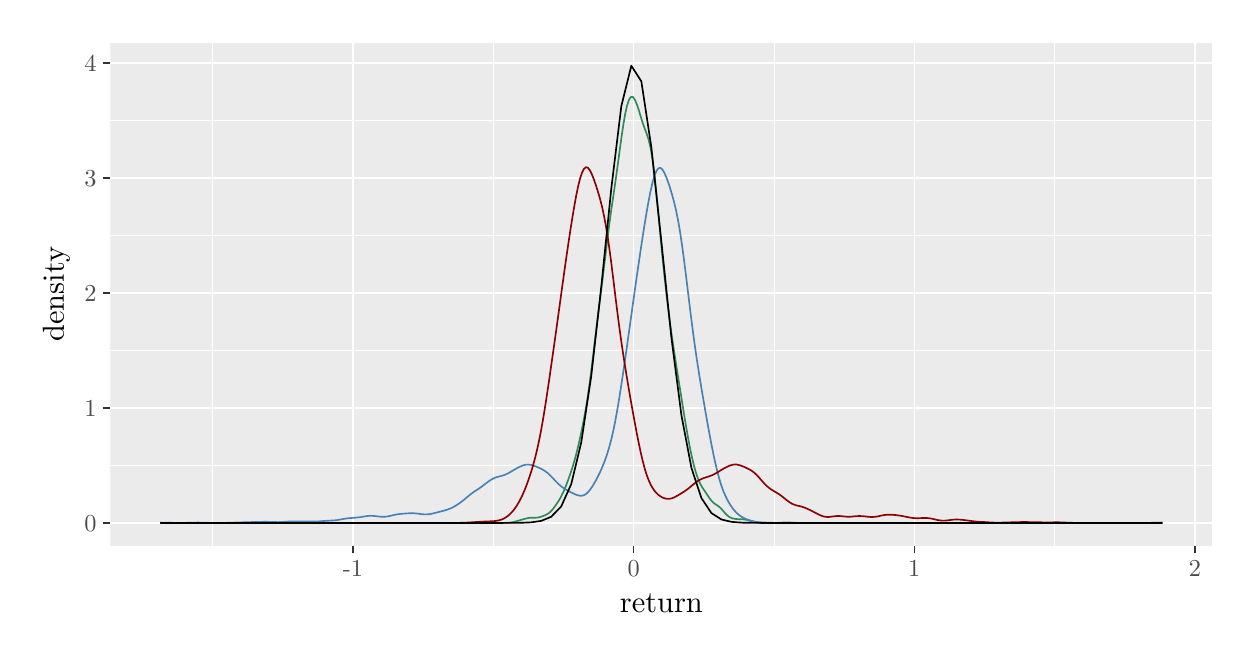
\begin{tikzpicture}[x=1pt,y=1pt]
\definecolor{fillColor}{RGB}{255,255,255}
\path[use as bounding box,fill=fillColor,fill opacity=0.00] (0,0) rectangle (433.62,216.81);
\begin{scope}
\path[clip] (  0.00,  0.00) rectangle (433.62,216.81);
\definecolor{drawColor}{RGB}{255,255,255}
\definecolor{fillColor}{RGB}{255,255,255}

\path[draw=drawColor,line width= 0.6pt,line join=round,line cap=round,fill=fillColor] (  0.00,  0.00) rectangle (433.62,216.81);
\end{scope}
\begin{scope}
\path[clip] ( 29.87, 29.59) rectangle (428.12,211.31);
\definecolor{fillColor}{gray}{0.92}

\path[fill=fillColor] ( 29.87, 29.59) rectangle (428.12,211.31);
\definecolor{drawColor}{RGB}{255,255,255}

\path[draw=drawColor,line width= 0.3pt,line join=round] ( 29.87, 58.62) --
	(428.12, 58.62);

\path[draw=drawColor,line width= 0.3pt,line join=round] ( 29.87,100.17) --
	(428.12,100.17);

\path[draw=drawColor,line width= 0.3pt,line join=round] ( 29.87,141.71) --
	(428.12,141.71);

\path[draw=drawColor,line width= 0.3pt,line join=round] ( 29.87,183.26) --
	(428.12,183.26);

\path[draw=drawColor,line width= 0.3pt,line join=round] ( 66.80, 29.59) --
	( 66.80,211.31);

\path[draw=drawColor,line width= 0.3pt,line join=round] (168.24, 29.59) --
	(168.24,211.31);

\path[draw=drawColor,line width= 0.3pt,line join=round] (269.68, 29.59) --
	(269.68,211.31);

\path[draw=drawColor,line width= 0.3pt,line join=round] (371.11, 29.59) --
	(371.11,211.31);

\path[draw=drawColor,line width= 0.6pt,line join=round] ( 29.87, 37.85) --
	(428.12, 37.85);

\path[draw=drawColor,line width= 0.6pt,line join=round] ( 29.87, 79.39) --
	(428.12, 79.39);

\path[draw=drawColor,line width= 0.6pt,line join=round] ( 29.87,120.94) --
	(428.12,120.94);

\path[draw=drawColor,line width= 0.6pt,line join=round] ( 29.87,162.49) --
	(428.12,162.49);

\path[draw=drawColor,line width= 0.6pt,line join=round] ( 29.87,204.03) --
	(428.12,204.03);

\path[draw=drawColor,line width= 0.6pt,line join=round] (117.52, 29.59) --
	(117.52,211.31);

\path[draw=drawColor,line width= 0.6pt,line join=round] (218.96, 29.59) --
	(218.96,211.31);

\path[draw=drawColor,line width= 0.6pt,line join=round] (320.39, 29.59) --
	(320.39,211.31);

\path[draw=drawColor,line width= 0.6pt,line join=round] (421.83, 29.59) --
	(421.83,211.31);
\definecolor{drawColor}{RGB}{46,139,87}

\path[draw=drawColor,line width= 0.6pt,line join=round] ( 47.97, 37.85) --
	( 48.68, 37.85) --
	( 49.39, 37.85) --
	( 50.10, 37.85) --
	( 50.81, 37.85) --
	( 51.51, 37.85) --
	( 52.22, 37.85) --
	( 52.93, 37.85) --
	( 53.64, 37.85) --
	( 54.35, 37.85) --
	( 55.06, 37.85) --
	( 55.76, 37.85) --
	( 56.47, 37.85) --
	( 57.18, 37.85) --
	( 57.89, 37.85) --
	( 58.60, 37.85) --
	( 59.31, 37.85) --
	( 60.02, 37.85) --
	( 60.72, 37.85) --
	( 61.43, 37.85) --
	( 62.14, 37.85) --
	( 62.85, 37.85) --
	( 63.56, 37.85) --
	( 64.27, 37.85) --
	( 64.98, 37.85) --
	( 65.68, 37.85) --
	( 66.39, 37.85) --
	( 67.10, 37.85) --
	( 67.81, 37.85) --
	( 68.52, 37.85) --
	( 69.23, 37.85) --
	( 69.93, 37.85) --
	( 70.64, 37.85) --
	( 71.35, 37.85) --
	( 72.06, 37.85) --
	( 72.77, 37.85) --
	( 73.48, 37.85) --
	( 74.19, 37.85) --
	( 74.89, 37.85) --
	( 75.60, 37.85) --
	( 76.31, 37.85) --
	( 77.02, 37.85) --
	( 77.73, 37.85) --
	( 78.44, 37.85) --
	( 79.15, 37.85) --
	( 79.85, 37.85) --
	( 80.56, 37.85) --
	( 81.27, 37.85) --
	( 81.98, 37.85) --
	( 82.69, 37.85) --
	( 83.40, 37.85) --
	( 84.10, 37.85) --
	( 84.81, 37.85) --
	( 85.52, 37.85) --
	( 86.23, 37.85) --
	( 86.94, 37.85) --
	( 87.65, 37.85) --
	( 88.36, 37.85) --
	( 89.06, 37.85) --
	( 89.77, 37.85) --
	( 90.48, 37.85) --
	( 91.19, 37.85) --
	( 91.90, 37.85) --
	( 92.61, 37.85) --
	( 93.32, 37.85) --
	( 94.02, 37.85) --
	( 94.73, 37.85) --
	( 95.44, 37.85) --
	( 96.15, 37.85) --
	( 96.86, 37.85) --
	( 97.57, 37.85) --
	( 98.28, 37.85) --
	( 98.98, 37.85) --
	( 99.69, 37.85) --
	(100.40, 37.85) --
	(101.11, 37.85) --
	(101.82, 37.85) --
	(102.53, 37.85) --
	(103.23, 37.85) --
	(103.94, 37.85) --
	(104.65, 37.85) --
	(105.36, 37.85) --
	(106.07, 37.85) --
	(106.78, 37.85) --
	(107.49, 37.85) --
	(108.19, 37.85) --
	(108.90, 37.85) --
	(109.61, 37.85) --
	(110.32, 37.85) --
	(111.03, 37.85) --
	(111.74, 37.85) --
	(112.45, 37.85) --
	(113.15, 37.85) --
	(113.86, 37.85) --
	(114.57, 37.85) --
	(115.28, 37.85) --
	(115.99, 37.85) --
	(116.70, 37.85) --
	(117.40, 37.85) --
	(118.11, 37.85) --
	(118.82, 37.85) --
	(119.53, 37.85) --
	(120.24, 37.85) --
	(120.95, 37.85) --
	(121.66, 37.85) --
	(122.36, 37.85) --
	(123.07, 37.85) --
	(123.78, 37.85) --
	(124.49, 37.85) --
	(125.20, 37.85) --
	(125.91, 37.85) --
	(126.62, 37.85) --
	(127.32, 37.85) --
	(128.03, 37.85) --
	(128.74, 37.85) --
	(129.45, 37.85) --
	(130.16, 37.85) --
	(130.87, 37.85) --
	(131.57, 37.85) --
	(132.28, 37.85) --
	(132.99, 37.85) --
	(133.70, 37.85) --
	(134.41, 37.85) --
	(135.12, 37.85) --
	(135.83, 37.85) --
	(136.53, 37.85) --
	(137.24, 37.85) --
	(137.95, 37.85) --
	(138.66, 37.85) --
	(139.37, 37.85) --
	(140.08, 37.85) --
	(140.79, 37.85) --
	(141.49, 37.85) --
	(142.20, 37.85) --
	(142.91, 37.85) --
	(143.62, 37.85) --
	(144.33, 37.85) --
	(145.04, 37.85) --
	(145.74, 37.85) --
	(146.45, 37.85) --
	(147.16, 37.85) --
	(147.87, 37.85) --
	(148.58, 37.85) --
	(149.29, 37.85) --
	(150.00, 37.85) --
	(150.70, 37.85) --
	(151.41, 37.85) --
	(152.12, 37.85) --
	(152.83, 37.85) --
	(153.54, 37.85) --
	(154.25, 37.85) --
	(154.96, 37.85) --
	(155.66, 37.85) --
	(156.37, 37.85) --
	(157.08, 37.85) --
	(157.79, 37.85) --
	(158.50, 37.86) --
	(159.21, 37.87) --
	(159.92, 37.89) --
	(160.62, 37.93) --
	(161.33, 37.97) --
	(162.04, 38.01) --
	(162.75, 38.03) --
	(163.46, 38.02) --
	(164.17, 38.00) --
	(164.87, 37.96) --
	(165.58, 37.92) --
	(166.29, 37.88) --
	(167.00, 37.86) --
	(167.71, 37.85) --
	(168.42, 37.85) --
	(169.13, 37.85) --
	(169.83, 37.85) --
	(170.54, 37.85) --
	(171.25, 37.85) --
	(171.96, 37.85) --
	(172.67, 37.87) --
	(173.38, 37.89) --
	(174.09, 37.95) --
	(174.79, 38.04) --
	(175.50, 38.18) --
	(176.21, 38.35) --
	(176.92, 38.55) --
	(177.63, 38.76) --
	(178.34, 38.97) --
	(179.04, 39.16) --
	(179.75, 39.35) --
	(180.46, 39.53) --
	(181.17, 39.67) --
	(181.88, 39.74) --
	(182.59, 39.74) --
	(183.30, 39.73) --
	(184.00, 39.76) --
	(184.71, 39.87) --
	(185.42, 40.06) --
	(186.13, 40.31) --
	(186.84, 40.59) --
	(187.55, 40.92) --
	(188.26, 41.35) --
	(188.96, 41.95) --
	(189.67, 42.72) --
	(190.38, 43.64) --
	(191.09, 44.65) --
	(191.80, 45.73) --
	(192.51, 46.92) --
	(193.21, 48.27) --
	(193.92, 49.81) --
	(194.63, 51.56) --
	(195.34, 53.46) --
	(196.05, 55.49) --
	(196.76, 57.64) --
	(197.47, 59.97) --
	(198.17, 62.53) --
	(198.88, 65.35) --
	(199.59, 68.45) --
	(200.30, 71.81) --
	(201.01, 75.44) --
	(201.72, 79.40) --
	(202.43, 83.82) --
	(203.13, 88.81) --
	(203.84, 94.36) --
	(204.55,100.28) --
	(205.26,106.28) --
	(205.97,112.07) --
	(206.68,117.64) --
	(207.39,123.17) --
	(208.09,128.86) --
	(208.80,134.75) --
	(209.51,140.63) --
	(210.22,146.18) --
	(210.93,151.28) --
	(211.64,156.10) --
	(212.34,160.94) --
	(213.05,166.00) --
	(213.76,171.26) --
	(214.47,176.49) --
	(215.18,181.37) --
	(215.89,185.54) --
	(216.60,188.75) --
	(217.30,190.84) --
	(218.01,191.81) --
	(218.72,191.74) --
	(219.43,190.77) --
	(220.14,189.08) --
	(220.85,186.92) --
	(221.56,184.56) --
	(222.26,182.32) --
	(222.97,180.34) --
	(223.68,178.49) --
	(224.39,176.31) --
	(225.10,173.28) --
	(225.81,168.97) --
	(226.51,163.33) --
	(227.22,156.61) --
	(227.93,149.23) --
	(228.64,141.66) --
	(229.35,134.28) --
	(230.06,127.33) --
	(230.77,120.90) --
	(231.47,114.98) --
	(232.18,109.53) --
	(232.89,104.47) --
	(233.60, 99.71) --
	(234.31, 95.15) --
	(235.02, 90.69) --
	(235.73, 86.25) --
	(236.43, 81.81) --
	(237.14, 77.38) --
	(237.85, 73.08) --
	(238.56, 69.00) --
	(239.27, 65.24) --
	(239.98, 61.85) --
	(240.68, 58.86) --
	(241.39, 56.28) --
	(242.10, 54.14) --
	(242.81, 52.43) --
	(243.52, 51.09) --
	(244.23, 49.97) --
	(244.94, 48.94) --
	(245.64, 47.88) --
	(246.35, 46.83) --
	(247.06, 45.89) --
	(247.77, 45.16) --
	(248.48, 44.63) --
	(249.19, 44.18) --
	(249.90, 43.66) --
	(250.60, 42.98) --
	(251.31, 42.18) --
	(252.02, 41.36) --
	(252.73, 40.64) --
	(253.44, 40.08) --
	(254.15, 39.69) --
	(254.85, 39.46) --
	(255.56, 39.32) --
	(256.27, 39.24) --
	(256.98, 39.20) --
	(257.69, 39.18) --
	(258.40, 39.16) --
	(259.11, 39.09) --
	(259.81, 38.96) --
	(260.52, 38.76) --
	(261.23, 38.54) --
	(261.94, 38.31) --
	(262.65, 38.13) --
	(263.36, 38.00) --
	(264.07, 37.92) --
	(264.77, 37.88) --
	(265.48, 37.86) --
	(266.19, 37.85) --
	(266.90, 37.85) --
	(267.61, 37.85) --
	(268.32, 37.85) --
	(269.03, 37.85) --
	(269.73, 37.85) --
	(270.44, 37.87) --
	(271.15, 37.89) --
	(271.86, 37.92) --
	(272.57, 37.96) --
	(273.28, 38.00) --
	(273.98, 38.03) --
	(274.69, 38.03) --
	(275.40, 38.00) --
	(276.11, 37.96) --
	(276.82, 37.92) --
	(277.53, 37.89) --
	(278.24, 37.87) --
	(278.94, 37.85) --
	(279.65, 37.85) --
	(280.36, 37.85) --
	(281.07, 37.85) --
	(281.78, 37.85) --
	(282.49, 37.85) --
	(283.20, 37.85) --
	(283.90, 37.85) --
	(284.61, 37.85) --
	(285.32, 37.85) --
	(286.03, 37.85) --
	(286.74, 37.85) --
	(287.45, 37.85) --
	(288.15, 37.85) --
	(288.86, 37.85) --
	(289.57, 37.85) --
	(290.28, 37.85) --
	(290.99, 37.85) --
	(291.70, 37.85) --
	(292.41, 37.85) --
	(293.11, 37.85) --
	(293.82, 37.85) --
	(294.53, 37.85) --
	(295.24, 37.85) --
	(295.95, 37.85) --
	(296.66, 37.85) --
	(297.37, 37.85) --
	(298.07, 37.85) --
	(298.78, 37.85) --
	(299.49, 37.85) --
	(300.20, 37.85) --
	(300.91, 37.85) --
	(301.62, 37.85) --
	(302.32, 37.85) --
	(303.03, 37.85) --
	(303.74, 37.85) --
	(304.45, 37.85) --
	(305.16, 37.85) --
	(305.87, 37.85) --
	(306.58, 37.85) --
	(307.28, 37.85) --
	(307.99, 37.85) --
	(308.70, 37.85) --
	(309.41, 37.85) --
	(310.12, 37.85) --
	(310.83, 37.85) --
	(311.54, 37.85) --
	(312.24, 37.85) --
	(312.95, 37.85) --
	(313.66, 37.85) --
	(314.37, 37.85) --
	(315.08, 37.85) --
	(315.79, 37.85) --
	(316.49, 37.85) --
	(317.20, 37.85) --
	(317.91, 37.85) --
	(318.62, 37.85) --
	(319.33, 37.85) --
	(320.04, 37.85) --
	(320.75, 37.85) --
	(321.45, 37.85) --
	(322.16, 37.85) --
	(322.87, 37.85) --
	(323.58, 37.85) --
	(324.29, 37.85) --
	(325.00, 37.85) --
	(325.71, 37.85) --
	(326.41, 37.85) --
	(327.12, 37.85) --
	(327.83, 37.85) --
	(328.54, 37.85) --
	(329.25, 37.85) --
	(329.96, 37.85) --
	(330.67, 37.85) --
	(331.37, 37.85) --
	(332.08, 37.85) --
	(332.79, 37.85) --
	(333.50, 37.85) --
	(334.21, 37.85) --
	(334.92, 37.85) --
	(335.62, 37.85) --
	(336.33, 37.85) --
	(337.04, 37.85) --
	(337.75, 37.85) --
	(338.46, 37.85) --
	(339.17, 37.85) --
	(339.88, 37.85) --
	(340.58, 37.85) --
	(341.29, 37.85) --
	(342.00, 37.85) --
	(342.71, 37.85) --
	(343.42, 37.85) --
	(344.13, 37.85) --
	(344.84, 37.85) --
	(345.54, 37.85) --
	(346.25, 37.85) --
	(346.96, 37.85) --
	(347.67, 37.85) --
	(348.38, 37.85) --
	(349.09, 37.85) --
	(349.79, 37.85) --
	(350.50, 37.85) --
	(351.21, 37.85) --
	(351.92, 37.85) --
	(352.63, 37.85) --
	(353.34, 37.85) --
	(354.05, 37.85) --
	(354.75, 37.85) --
	(355.46, 37.85) --
	(356.17, 37.85) --
	(356.88, 37.85) --
	(357.59, 37.85) --
	(358.30, 37.85) --
	(359.01, 37.85) --
	(359.71, 37.85) --
	(360.42, 37.85) --
	(361.13, 37.85) --
	(361.84, 37.85) --
	(362.55, 37.85) --
	(363.26, 37.85) --
	(363.96, 37.85) --
	(364.67, 37.85) --
	(365.38, 37.85) --
	(366.09, 37.85) --
	(366.80, 37.85) --
	(367.51, 37.85) --
	(368.22, 37.85) --
	(368.92, 37.85) --
	(369.63, 37.85) --
	(370.34, 37.85) --
	(371.05, 37.85) --
	(371.76, 37.85) --
	(372.47, 37.85) --
	(373.18, 37.85) --
	(373.88, 37.85) --
	(374.59, 37.85) --
	(375.30, 37.85) --
	(376.01, 37.85) --
	(376.72, 37.85) --
	(377.43, 37.85) --
	(378.13, 37.85) --
	(378.84, 37.85) --
	(379.55, 37.85) --
	(380.26, 37.85) --
	(380.97, 37.85) --
	(381.68, 37.85) --
	(382.39, 37.85) --
	(383.09, 37.85) --
	(383.80, 37.85) --
	(384.51, 37.85) --
	(385.22, 37.85) --
	(385.93, 37.85) --
	(386.64, 37.85) --
	(387.35, 37.85) --
	(388.05, 37.85) --
	(388.76, 37.85) --
	(389.47, 37.85) --
	(390.18, 37.85) --
	(390.89, 37.85) --
	(391.60, 37.85) --
	(392.31, 37.85) --
	(393.01, 37.85) --
	(393.72, 37.85) --
	(394.43, 37.85) --
	(395.14, 37.85) --
	(395.85, 37.85) --
	(396.56, 37.85) --
	(397.26, 37.85) --
	(397.97, 37.85) --
	(398.68, 37.85) --
	(399.39, 37.85) --
	(400.10, 37.85) --
	(400.81, 37.85) --
	(401.52, 37.85) --
	(402.22, 37.85) --
	(402.93, 37.85) --
	(403.64, 37.85) --
	(404.35, 37.85) --
	(405.06, 37.85) --
	(405.77, 37.85) --
	(406.48, 37.85) --
	(407.18, 37.85) --
	(407.89, 37.85) --
	(408.60, 37.85) --
	(409.31, 37.85) --
	(410.02, 37.85);
\definecolor{drawColor}{RGB}{70,130,180}

\path[draw=drawColor,line width= 0.6pt,line join=round] ( 47.97, 37.98) --
	( 48.68, 37.97) --
	( 49.39, 37.96) --
	( 50.10, 37.94) --
	( 50.81, 37.92) --
	( 51.51, 37.90) --
	( 52.22, 37.88) --
	( 52.93, 37.87) --
	( 53.64, 37.86) --
	( 54.35, 37.86) --
	( 55.06, 37.86) --
	( 55.76, 37.86) --
	( 56.47, 37.87) --
	( 57.18, 37.88) --
	( 57.89, 37.90) --
	( 58.60, 37.91) --
	( 59.31, 37.94) --
	( 60.02, 37.96) --
	( 60.72, 37.97) --
	( 61.43, 37.98) --
	( 62.14, 37.97) --
	( 62.85, 37.96) --
	( 63.56, 37.94) --
	( 64.27, 37.92) --
	( 64.98, 37.90) --
	( 65.68, 37.88) --
	( 66.39, 37.87) --
	( 67.10, 37.86) --
	( 67.81, 37.86) --
	( 68.52, 37.85) --
	( 69.23, 37.85) --
	( 69.93, 37.86) --
	( 70.64, 37.86) --
	( 71.35, 37.87) --
	( 72.06, 37.89) --
	( 72.77, 37.91) --
	( 73.48, 37.93) --
	( 74.19, 37.96) --
	( 74.89, 37.98) --
	( 75.60, 38.01) --
	( 76.31, 38.03) --
	( 77.02, 38.05) --
	( 77.73, 38.07) --
	( 78.44, 38.09) --
	( 79.15, 38.12) --
	( 79.85, 38.14) --
	( 80.56, 38.15) --
	( 81.27, 38.17) --
	( 81.98, 38.18) --
	( 82.69, 38.19) --
	( 83.40, 38.20) --
	( 84.10, 38.22) --
	( 84.81, 38.24) --
	( 85.52, 38.26) --
	( 86.23, 38.26) --
	( 86.94, 38.25) --
	( 87.65, 38.23) --
	( 88.36, 38.20) --
	( 89.06, 38.18) --
	( 89.77, 38.16) --
	( 90.48, 38.15) --
	( 91.19, 38.17) --
	( 91.90, 38.20) --
	( 92.61, 38.24) --
	( 93.32, 38.29) --
	( 94.02, 38.33) --
	( 94.73, 38.36) --
	( 95.44, 38.38) --
	( 96.15, 38.39) --
	( 96.86, 38.39) --
	( 97.57, 38.39) --
	( 98.28, 38.40) --
	( 98.98, 38.40) --
	( 99.69, 38.41) --
	(100.40, 38.40) --
	(101.11, 38.39) --
	(101.82, 38.38) --
	(102.53, 38.37) --
	(103.23, 38.36) --
	(103.94, 38.36) --
	(104.65, 38.38) --
	(105.36, 38.42) --
	(106.07, 38.47) --
	(106.78, 38.53) --
	(107.49, 38.58) --
	(108.19, 38.63) --
	(108.90, 38.67) --
	(109.61, 38.70) --
	(110.32, 38.74) --
	(111.03, 38.80) --
	(111.74, 38.88) --
	(112.45, 38.99) --
	(113.15, 39.11) --
	(113.86, 39.24) --
	(114.57, 39.37) --
	(115.28, 39.47) --
	(115.99, 39.56) --
	(116.70, 39.62) --
	(117.40, 39.67) --
	(118.11, 39.72) --
	(118.82, 39.78) --
	(119.53, 39.86) --
	(120.24, 39.95) --
	(120.95, 40.07) --
	(121.66, 40.19) --
	(122.36, 40.30) --
	(123.07, 40.38) --
	(123.78, 40.42) --
	(124.49, 40.41) --
	(125.20, 40.36) --
	(125.91, 40.28) --
	(126.62, 40.19) --
	(127.32, 40.12) --
	(128.03, 40.07) --
	(128.74, 40.07) --
	(129.45, 40.12) --
	(130.16, 40.23) --
	(130.87, 40.37) --
	(131.57, 40.54) --
	(132.28, 40.70) --
	(132.99, 40.86) --
	(133.70, 40.98) --
	(134.41, 41.07) --
	(135.12, 41.14) --
	(135.83, 41.20) --
	(136.53, 41.25) --
	(137.24, 41.30) --
	(137.95, 41.34) --
	(138.66, 41.36) --
	(139.37, 41.34) --
	(140.08, 41.30) --
	(140.79, 41.23) --
	(141.49, 41.14) --
	(142.20, 41.04) --
	(142.91, 40.97) --
	(143.62, 40.93) --
	(144.33, 40.95) --
	(145.04, 41.01) --
	(145.74, 41.12) --
	(146.45, 41.27) --
	(147.16, 41.45) --
	(147.87, 41.63) --
	(148.58, 41.82) --
	(149.29, 42.00) --
	(150.00, 42.18) --
	(150.70, 42.37) --
	(151.41, 42.58) --
	(152.12, 42.83) --
	(152.83, 43.11) --
	(153.54, 43.45) --
	(154.25, 43.83) --
	(154.96, 44.25) --
	(155.66, 44.72) --
	(156.37, 45.22) --
	(157.08, 45.76) --
	(157.79, 46.33) --
	(158.50, 46.92) --
	(159.21, 47.51) --
	(159.92, 48.09) --
	(160.62, 48.63) --
	(161.33, 49.13) --
	(162.04, 49.60) --
	(162.75, 50.06) --
	(163.46, 50.54) --
	(164.17, 51.05) --
	(164.87, 51.59) --
	(165.58, 52.14) --
	(166.29, 52.67) --
	(167.00, 53.17) --
	(167.71, 53.60) --
	(168.42, 53.96) --
	(169.13, 54.25) --
	(169.83, 54.48) --
	(170.54, 54.68) --
	(171.25, 54.87) --
	(171.96, 55.08) --
	(172.67, 55.35) --
	(173.38, 55.67) --
	(174.09, 56.05) --
	(174.79, 56.46) --
	(175.50, 56.88) --
	(176.21, 57.29) --
	(176.92, 57.69) --
	(177.63, 58.06) --
	(178.34, 58.38) --
	(179.04, 58.65) --
	(179.75, 58.84) --
	(180.46, 58.93) --
	(181.17, 58.92) --
	(181.88, 58.81) --
	(182.59, 58.63) --
	(183.30, 58.38) --
	(184.00, 58.11) --
	(184.71, 57.80) --
	(185.42, 57.47) --
	(186.13, 57.09) --
	(186.84, 56.66) --
	(187.55, 56.15) --
	(188.26, 55.56) --
	(188.96, 54.88) --
	(189.67, 54.14) --
	(190.38, 53.37) --
	(191.09, 52.62) --
	(191.80, 51.92) --
	(192.51, 51.29) --
	(193.21, 50.74) --
	(193.92, 50.26) --
	(194.63, 49.83) --
	(195.34, 49.43) --
	(196.05, 49.06) --
	(196.76, 48.69) --
	(197.47, 48.35) --
	(198.17, 48.05) --
	(198.88, 47.82) --
	(199.59, 47.68) --
	(200.30, 47.69) --
	(201.01, 47.88) --
	(201.72, 48.29) --
	(202.43, 48.91) --
	(203.13, 49.74) --
	(203.84, 50.74) --
	(204.55, 51.87) --
	(205.26, 53.11) --
	(205.97, 54.45) --
	(206.68, 55.88) --
	(207.39, 57.44) --
	(208.09, 59.14) --
	(208.80, 61.02) --
	(209.51, 63.12) --
	(210.22, 65.49) --
	(210.93, 68.20) --
	(211.64, 71.28) --
	(212.34, 74.77) --
	(213.05, 78.66) --
	(213.76, 82.91) --
	(214.47, 87.43) --
	(215.18, 92.16) --
	(215.89, 97.03) --
	(216.60,101.99) --
	(217.30,107.01) --
	(218.01,112.07) --
	(218.72,117.14) --
	(219.43,122.19) --
	(220.14,127.18) --
	(220.85,132.08) --
	(221.56,136.87) --
	(222.26,141.52) --
	(222.97,146.01) --
	(223.68,150.28) --
	(224.39,154.27) --
	(225.10,157.86) --
	(225.81,160.94) --
	(226.51,163.38) --
	(227.22,165.09) --
	(227.93,166.01) --
	(228.64,166.16) --
	(229.35,165.57) --
	(230.06,164.38) --
	(230.77,162.75) --
	(231.47,160.83) --
	(232.18,158.68) --
	(232.89,156.32) --
	(233.60,153.69) --
	(234.31,150.69) --
	(235.02,147.18) --
	(235.73,143.08) --
	(236.43,138.36) --
	(237.14,133.10) --
	(237.85,127.45) --
	(238.56,121.61) --
	(239.27,115.78) --
	(239.98,110.13) --
	(240.68,104.76) --
	(241.39, 99.72) --
	(242.10, 94.97) --
	(242.81, 90.49) --
	(243.52, 86.18) --
	(244.23, 82.01) --
	(244.94, 77.92) --
	(245.64, 73.93) --
	(246.35, 70.04) --
	(247.06, 66.30) --
	(247.77, 62.75) --
	(248.48, 59.47) --
	(249.19, 56.48) --
	(249.90, 53.84) --
	(250.60, 51.54) --
	(251.31, 49.55) --
	(252.02, 47.85) --
	(252.73, 46.38) --
	(253.44, 45.11) --
	(254.15, 43.98) --
	(254.85, 42.99) --
	(255.56, 42.13) --
	(256.27, 41.39) --
	(256.98, 40.76) --
	(257.69, 40.25) --
	(258.40, 39.82) --
	(259.11, 39.47) --
	(259.81, 39.17) --
	(260.52, 38.92) --
	(261.23, 38.70) --
	(261.94, 38.51) --
	(262.65, 38.36) --
	(263.36, 38.24) --
	(264.07, 38.15) --
	(264.77, 38.09) --
	(265.48, 38.04) --
	(266.19, 38.00) --
	(266.90, 37.97) --
	(267.61, 37.94) --
	(268.32, 37.91) --
	(269.03, 37.89) --
	(269.73, 37.87) --
	(270.44, 37.86) --
	(271.15, 37.86) --
	(271.86, 37.85) --
	(272.57, 37.85) --
	(273.28, 37.85) --
	(273.98, 37.85) --
	(274.69, 37.85) --
	(275.40, 37.85) --
	(276.11, 37.85) --
	(276.82, 37.85) --
	(277.53, 37.85) --
	(278.24, 37.85) --
	(278.94, 37.85) --
	(279.65, 37.85) --
	(280.36, 37.85) --
	(281.07, 37.85) --
	(281.78, 37.85) --
	(282.49, 37.85) --
	(283.20, 37.85) --
	(283.90, 37.85) --
	(284.61, 37.85) --
	(285.32, 37.85) --
	(286.03, 37.85) --
	(286.74, 37.85) --
	(287.45, 37.85) --
	(288.15, 37.85) --
	(288.86, 37.85) --
	(289.57, 37.85) --
	(290.28, 37.85) --
	(290.99, 37.85) --
	(291.70, 37.85) --
	(292.41, 37.85) --
	(293.11, 37.85) --
	(293.82, 37.85) --
	(294.53, 37.85) --
	(295.24, 37.85) --
	(295.95, 37.85) --
	(296.66, 37.85) --
	(297.37, 37.85) --
	(298.07, 37.85) --
	(298.78, 37.85) --
	(299.49, 37.85) --
	(300.20, 37.85) --
	(300.91, 37.85) --
	(301.62, 37.85) --
	(302.32, 37.85) --
	(303.03, 37.85) --
	(303.74, 37.85) --
	(304.45, 37.85) --
	(305.16, 37.85) --
	(305.87, 37.85) --
	(306.58, 37.85) --
	(307.28, 37.85) --
	(307.99, 37.85) --
	(308.70, 37.85) --
	(309.41, 37.85) --
	(310.12, 37.85) --
	(310.83, 37.85) --
	(311.54, 37.85) --
	(312.24, 37.85) --
	(312.95, 37.85) --
	(313.66, 37.85) --
	(314.37, 37.85) --
	(315.08, 37.85) --
	(315.79, 37.85) --
	(316.49, 37.85) --
	(317.20, 37.85) --
	(317.91, 37.85) --
	(318.62, 37.85) --
	(319.33, 37.85) --
	(320.04, 37.85) --
	(320.75, 37.85) --
	(321.45, 37.85) --
	(322.16, 37.85) --
	(322.87, 37.85) --
	(323.58, 37.85) --
	(324.29, 37.85) --
	(325.00, 37.85) --
	(325.71, 37.85) --
	(326.41, 37.85) --
	(327.12, 37.85) --
	(327.83, 37.85) --
	(328.54, 37.85) --
	(329.25, 37.85) --
	(329.96, 37.85) --
	(330.67, 37.85) --
	(331.37, 37.85) --
	(332.08, 37.85) --
	(332.79, 37.85) --
	(333.50, 37.85) --
	(334.21, 37.85) --
	(334.92, 37.85) --
	(335.62, 37.85) --
	(336.33, 37.85) --
	(337.04, 37.85) --
	(337.75, 37.85) --
	(338.46, 37.85) --
	(339.17, 37.85) --
	(339.88, 37.85) --
	(340.58, 37.85) --
	(341.29, 37.85) --
	(342.00, 37.85) --
	(342.71, 37.85) --
	(343.42, 37.85) --
	(344.13, 37.85) --
	(344.84, 37.85) --
	(345.54, 37.85) --
	(346.25, 37.85) --
	(346.96, 37.85) --
	(347.67, 37.85) --
	(348.38, 37.85) --
	(349.09, 37.85) --
	(349.79, 37.85) --
	(350.50, 37.85) --
	(351.21, 37.85) --
	(351.92, 37.85) --
	(352.63, 37.85) --
	(353.34, 37.85) --
	(354.05, 37.85) --
	(354.75, 37.85) --
	(355.46, 37.85) --
	(356.17, 37.85) --
	(356.88, 37.85) --
	(357.59, 37.85) --
	(358.30, 37.85) --
	(359.01, 37.85) --
	(359.71, 37.85) --
	(360.42, 37.85) --
	(361.13, 37.85) --
	(361.84, 37.85) --
	(362.55, 37.85) --
	(363.26, 37.85) --
	(363.96, 37.85) --
	(364.67, 37.85) --
	(365.38, 37.85) --
	(366.09, 37.85) --
	(366.80, 37.85) --
	(367.51, 37.85) --
	(368.22, 37.85) --
	(368.92, 37.85) --
	(369.63, 37.85) --
	(370.34, 37.85) --
	(371.05, 37.85) --
	(371.76, 37.85) --
	(372.47, 37.85) --
	(373.18, 37.85) --
	(373.88, 37.85) --
	(374.59, 37.85) --
	(375.30, 37.85) --
	(376.01, 37.85) --
	(376.72, 37.85) --
	(377.43, 37.85) --
	(378.13, 37.85) --
	(378.84, 37.85) --
	(379.55, 37.85) --
	(380.26, 37.85) --
	(380.97, 37.85) --
	(381.68, 37.85) --
	(382.39, 37.85) --
	(383.09, 37.85) --
	(383.80, 37.85) --
	(384.51, 37.85) --
	(385.22, 37.85) --
	(385.93, 37.85) --
	(386.64, 37.85) --
	(387.35, 37.85) --
	(388.05, 37.85) --
	(388.76, 37.85) --
	(389.47, 37.85) --
	(390.18, 37.85) --
	(390.89, 37.85) --
	(391.60, 37.85) --
	(392.31, 37.85) --
	(393.01, 37.85) --
	(393.72, 37.85) --
	(394.43, 37.85) --
	(395.14, 37.85) --
	(395.85, 37.85) --
	(396.56, 37.85) --
	(397.26, 37.85) --
	(397.97, 37.85) --
	(398.68, 37.85) --
	(399.39, 37.85) --
	(400.10, 37.85) --
	(400.81, 37.85) --
	(401.52, 37.85) --
	(402.22, 37.85) --
	(402.93, 37.85) --
	(403.64, 37.85) --
	(404.35, 37.85) --
	(405.06, 37.85) --
	(405.77, 37.85) --
	(406.48, 37.85) --
	(407.18, 37.85) --
	(407.89, 37.85) --
	(408.60, 37.85) --
	(409.31, 37.85) --
	(410.02, 37.85);
\definecolor{drawColor}{RGB}{139,0,0}

\path[draw=drawColor,line width= 0.6pt,line join=round] ( 47.97, 37.85) --
	( 48.68, 37.85) --
	( 49.39, 37.85) --
	( 50.10, 37.85) --
	( 50.81, 37.85) --
	( 51.51, 37.85) --
	( 52.22, 37.85) --
	( 52.93, 37.85) --
	( 53.64, 37.85) --
	( 54.35, 37.85) --
	( 55.06, 37.85) --
	( 55.76, 37.85) --
	( 56.47, 37.85) --
	( 57.18, 37.85) --
	( 57.89, 37.85) --
	( 58.60, 37.85) --
	( 59.31, 37.85) --
	( 60.02, 37.85) --
	( 60.72, 37.85) --
	( 61.43, 37.85) --
	( 62.14, 37.85) --
	( 62.85, 37.85) --
	( 63.56, 37.85) --
	( 64.27, 37.85) --
	( 64.98, 37.85) --
	( 65.68, 37.85) --
	( 66.39, 37.85) --
	( 67.10, 37.85) --
	( 67.81, 37.85) --
	( 68.52, 37.85) --
	( 69.23, 37.85) --
	( 69.93, 37.85) --
	( 70.64, 37.85) --
	( 71.35, 37.85) --
	( 72.06, 37.85) --
	( 72.77, 37.85) --
	( 73.48, 37.85) --
	( 74.19, 37.85) --
	( 74.89, 37.85) --
	( 75.60, 37.85) --
	( 76.31, 37.85) --
	( 77.02, 37.85) --
	( 77.73, 37.85) --
	( 78.44, 37.85) --
	( 79.15, 37.85) --
	( 79.85, 37.85) --
	( 80.56, 37.85) --
	( 81.27, 37.85) --
	( 81.98, 37.85) --
	( 82.69, 37.85) --
	( 83.40, 37.85) --
	( 84.10, 37.85) --
	( 84.81, 37.85) --
	( 85.52, 37.85) --
	( 86.23, 37.85) --
	( 86.94, 37.85) --
	( 87.65, 37.85) --
	( 88.36, 37.85) --
	( 89.06, 37.85) --
	( 89.77, 37.85) --
	( 90.48, 37.85) --
	( 91.19, 37.85) --
	( 91.90, 37.85) --
	( 92.61, 37.85) --
	( 93.32, 37.85) --
	( 94.02, 37.85) --
	( 94.73, 37.85) --
	( 95.44, 37.85) --
	( 96.15, 37.85) --
	( 96.86, 37.85) --
	( 97.57, 37.85) --
	( 98.28, 37.85) --
	( 98.98, 37.85) --
	( 99.69, 37.85) --
	(100.40, 37.85) --
	(101.11, 37.85) --
	(101.82, 37.85) --
	(102.53, 37.85) --
	(103.23, 37.85) --
	(103.94, 37.85) --
	(104.65, 37.85) --
	(105.36, 37.85) --
	(106.07, 37.85) --
	(106.78, 37.85) --
	(107.49, 37.85) --
	(108.19, 37.85) --
	(108.90, 37.85) --
	(109.61, 37.85) --
	(110.32, 37.85) --
	(111.03, 37.85) --
	(111.74, 37.85) --
	(112.45, 37.85) --
	(113.15, 37.85) --
	(113.86, 37.85) --
	(114.57, 37.85) --
	(115.28, 37.85) --
	(115.99, 37.85) --
	(116.70, 37.85) --
	(117.40, 37.85) --
	(118.11, 37.85) --
	(118.82, 37.85) --
	(119.53, 37.85) --
	(120.24, 37.85) --
	(120.95, 37.85) --
	(121.66, 37.85) --
	(122.36, 37.85) --
	(123.07, 37.85) --
	(123.78, 37.85) --
	(124.49, 37.85) --
	(125.20, 37.85) --
	(125.91, 37.85) --
	(126.62, 37.85) --
	(127.32, 37.85) --
	(128.03, 37.85) --
	(128.74, 37.85) --
	(129.45, 37.85) --
	(130.16, 37.85) --
	(130.87, 37.85) --
	(131.57, 37.85) --
	(132.28, 37.85) --
	(132.99, 37.85) --
	(133.70, 37.85) --
	(134.41, 37.85) --
	(135.12, 37.85) --
	(135.83, 37.85) --
	(136.53, 37.85) --
	(137.24, 37.85) --
	(137.95, 37.85) --
	(138.66, 37.85) --
	(139.37, 37.85) --
	(140.08, 37.85) --
	(140.79, 37.85) --
	(141.49, 37.85) --
	(142.20, 37.85) --
	(142.91, 37.85) --
	(143.62, 37.85) --
	(144.33, 37.85) --
	(145.04, 37.85) --
	(145.74, 37.85) --
	(146.45, 37.85) --
	(147.16, 37.85) --
	(147.87, 37.85) --
	(148.58, 37.85) --
	(149.29, 37.85) --
	(150.00, 37.85) --
	(150.70, 37.85) --
	(151.41, 37.85) --
	(152.12, 37.85) --
	(152.83, 37.85) --
	(153.54, 37.85) --
	(154.25, 37.85) --
	(154.96, 37.86) --
	(155.66, 37.87) --
	(156.37, 37.89) --
	(157.08, 37.91) --
	(157.79, 37.94) --
	(158.50, 37.97) --
	(159.21, 38.00) --
	(159.92, 38.04) --
	(160.62, 38.08) --
	(161.33, 38.13) --
	(162.04, 38.17) --
	(162.75, 38.22) --
	(163.46, 38.27) --
	(164.17, 38.31) --
	(164.87, 38.34) --
	(165.58, 38.37) --
	(166.29, 38.40) --
	(167.00, 38.42) --
	(167.71, 38.45) --
	(168.42, 38.50) --
	(169.13, 38.57) --
	(169.83, 38.69) --
	(170.54, 38.85) --
	(171.25, 39.08) --
	(171.96, 39.38) --
	(172.67, 39.78) --
	(173.38, 40.27) --
	(174.09, 40.86) --
	(174.79, 41.56) --
	(175.50, 42.37) --
	(176.21, 43.31) --
	(176.92, 44.39) --
	(177.63, 45.60) --
	(178.34, 46.97) --
	(179.04, 48.49) --
	(179.75, 50.17) --
	(180.46, 52.01) --
	(181.17, 54.01) --
	(181.88, 56.17) --
	(182.59, 58.53) --
	(183.30, 61.12) --
	(184.00, 63.99) --
	(184.71, 67.20) --
	(185.42, 70.77) --
	(186.13, 74.72) --
	(186.84, 79.01) --
	(187.55, 83.58) --
	(188.26, 88.33) --
	(188.96, 93.19) --
	(189.67, 98.14) --
	(190.38,103.15) --
	(191.09,108.22) --
	(191.80,113.35) --
	(192.51,118.51) --
	(193.21,123.65) --
	(193.92,128.74) --
	(194.63,133.73) --
	(195.34,138.58) --
	(196.05,143.27) --
	(196.76,147.77) --
	(197.47,152.01) --
	(198.17,155.91) --
	(198.88,159.36) --
	(199.59,162.23) --
	(200.30,164.40) --
	(201.01,165.80) --
	(201.72,166.39) --
	(202.43,166.20) --
	(203.13,165.30) --
	(203.84,163.88) --
	(204.55,162.09) --
	(205.26,160.06) --
	(205.97,157.85) --
	(206.68,155.44) --
	(207.39,152.75) --
	(208.09,149.63) --
	(208.80,145.96) --
	(209.51,141.68) --
	(210.22,136.79) --
	(210.93,131.41) --
	(211.64,125.72) --
	(212.34,119.93) --
	(213.05,114.24) --
	(213.76,108.80) --
	(214.47,103.66) --
	(215.18, 98.84) --
	(215.89, 94.28) --
	(216.60, 89.94) --
	(217.30, 85.75) --
	(218.01, 81.66) --
	(218.72, 77.67) --
	(219.43, 73.78) --
	(220.14, 70.03) --
	(220.85, 66.47) --
	(221.56, 63.15) --
	(222.26, 60.14) --
	(222.97, 57.48) --
	(223.68, 55.20) --
	(224.39, 53.29) --
	(225.10, 51.73) --
	(225.81, 50.47) --
	(226.51, 49.45) --
	(227.22, 48.64) --
	(227.93, 47.98) --
	(228.64, 47.45) --
	(229.35, 47.05) --
	(230.06, 46.77) --
	(230.77, 46.59) --
	(231.47, 46.54) --
	(232.18, 46.61) --
	(232.89, 46.79) --
	(233.60, 47.08) --
	(234.31, 47.44) --
	(235.02, 47.84) --
	(235.73, 48.27) --
	(236.43, 48.70) --
	(237.14, 49.15) --
	(237.85, 49.63) --
	(238.56, 50.15) --
	(239.27, 50.71) --
	(239.98, 51.30) --
	(240.68, 51.89) --
	(241.39, 52.45) --
	(242.10, 52.96) --
	(242.81, 53.39) --
	(243.52, 53.75) --
	(244.23, 54.03) --
	(244.94, 54.28) --
	(245.64, 54.49) --
	(246.35, 54.72) --
	(247.06, 54.99) --
	(247.77, 55.31) --
	(248.48, 55.68) --
	(249.19, 56.09) --
	(249.90, 56.53) --
	(250.60, 56.96) --
	(251.31, 57.37) --
	(252.02, 57.77) --
	(252.73, 58.13) --
	(253.44, 58.46) --
	(254.15, 58.72) --
	(254.85, 58.90) --
	(255.56, 58.97) --
	(256.27, 58.93) --
	(256.98, 58.78) --
	(257.69, 58.57) --
	(258.40, 58.30) --
	(259.11, 58.00) --
	(259.81, 57.67) --
	(260.52, 57.32) --
	(261.23, 56.92) --
	(261.94, 56.46) --
	(262.65, 55.90) --
	(263.36, 55.24) --
	(264.07, 54.50) --
	(264.77, 53.69) --
	(265.48, 52.87) --
	(266.19, 52.07) --
	(266.90, 51.35) --
	(267.61, 50.73) --
	(268.32, 50.19) --
	(269.03, 49.73) --
	(269.73, 49.31) --
	(270.44, 48.89) --
	(271.15, 48.45) --
	(271.86, 47.97) --
	(272.57, 47.45) --
	(273.28, 46.89) --
	(273.98, 46.31) --
	(274.69, 45.76) --
	(275.40, 45.26) --
	(276.11, 44.83) --
	(276.82, 44.50) --
	(277.53, 44.26) --
	(278.24, 44.08) --
	(278.94, 43.92) --
	(279.65, 43.74) --
	(280.36, 43.51) --
	(281.07, 43.24) --
	(281.78, 42.93) --
	(282.49, 42.60) --
	(283.20, 42.25) --
	(283.90, 41.89) --
	(284.61, 41.52) --
	(285.32, 41.15) --
	(286.03, 40.80) --
	(286.74, 40.49) --
	(287.45, 40.24) --
	(288.15, 40.08) --
	(288.86, 40.01) --
	(289.57, 40.02) --
	(290.28, 40.09) --
	(290.99, 40.19) --
	(291.70, 40.28) --
	(292.41, 40.34) --
	(293.11, 40.35) --
	(293.82, 40.31) --
	(294.53, 40.24) --
	(295.24, 40.16) --
	(295.95, 40.11) --
	(296.66, 40.08) --
	(297.37, 40.11) --
	(298.07, 40.16) --
	(298.78, 40.23) --
	(299.49, 40.29) --
	(300.20, 40.33) --
	(300.91, 40.33) --
	(301.62, 40.29) --
	(302.32, 40.23) --
	(303.03, 40.15) --
	(303.74, 40.07) --
	(304.45, 40.02) --
	(305.16, 40.00) --
	(305.87, 40.03) --
	(306.58, 40.11) --
	(307.28, 40.24) --
	(307.99, 40.39) --
	(308.70, 40.55) --
	(309.41, 40.68) --
	(310.12, 40.77) --
	(310.83, 40.82) --
	(311.54, 40.83) --
	(312.24, 40.80) --
	(312.95, 40.75) --
	(313.66, 40.69) --
	(314.37, 40.60) --
	(315.08, 40.50) --
	(315.79, 40.39) --
	(316.49, 40.25) --
	(317.20, 40.11) --
	(317.91, 39.96) --
	(318.62, 39.82) --
	(319.33, 39.70) --
	(320.04, 39.61) --
	(320.75, 39.56) --
	(321.45, 39.55) --
	(322.16, 39.57) --
	(322.87, 39.60) --
	(323.58, 39.63) --
	(324.29, 39.64) --
	(325.00, 39.62) --
	(325.71, 39.55) --
	(326.41, 39.44) --
	(327.12, 39.29) --
	(327.83, 39.13) --
	(328.54, 38.96) --
	(329.25, 38.82) --
	(329.96, 38.72) --
	(330.67, 38.67) --
	(331.37, 38.68) --
	(332.08, 38.74) --
	(332.79, 38.83) --
	(333.50, 38.92) --
	(334.21, 39.01) --
	(334.92, 39.06) --
	(335.62, 39.08) --
	(336.33, 39.07) --
	(337.04, 39.02) --
	(337.75, 38.96) --
	(338.46, 38.88) --
	(339.17, 38.79) --
	(339.88, 38.69) --
	(340.58, 38.60) --
	(341.29, 38.50) --
	(342.00, 38.41) --
	(342.71, 38.34) --
	(343.42, 38.28) --
	(344.13, 38.24) --
	(344.84, 38.20) --
	(345.54, 38.17) --
	(346.25, 38.13) --
	(346.96, 38.09) --
	(347.67, 38.04) --
	(348.38, 38.00) --
	(349.09, 37.97) --
	(349.79, 37.95) --
	(350.50, 37.94) --
	(351.21, 37.95) --
	(351.92, 37.97) --
	(352.63, 37.99) --
	(353.34, 38.01) --
	(354.05, 38.03) --
	(354.75, 38.05) --
	(355.46, 38.07) --
	(356.17, 38.09) --
	(356.88, 38.11) --
	(357.59, 38.13) --
	(358.30, 38.15) --
	(359.01, 38.16) --
	(359.71, 38.16) --
	(360.42, 38.16) --
	(361.13, 38.16) --
	(361.84, 38.15) --
	(362.55, 38.15) --
	(363.26, 38.15) --
	(363.96, 38.14) --
	(364.67, 38.13) --
	(365.38, 38.10) --
	(366.09, 38.08) --
	(366.80, 38.05) --
	(367.51, 38.04) --
	(368.22, 38.03) --
	(368.92, 38.03) --
	(369.63, 38.04) --
	(370.34, 38.06) --
	(371.05, 38.07) --
	(371.76, 38.07) --
	(372.47, 38.07) --
	(373.18, 38.06) --
	(373.88, 38.03) --
	(374.59, 38.00) --
	(375.30, 37.97) --
	(376.01, 37.94) --
	(376.72, 37.91) --
	(377.43, 37.89) --
	(378.13, 37.87) --
	(378.84, 37.86) --
	(379.55, 37.86) --
	(380.26, 37.85) --
	(380.97, 37.85) --
	(381.68, 37.85) --
	(382.39, 37.85) --
	(383.09, 37.85) --
	(383.80, 37.85) --
	(384.51, 37.85) --
	(385.22, 37.85) --
	(385.93, 37.85) --
	(386.64, 37.85) --
	(387.35, 37.85) --
	(388.05, 37.85) --
	(388.76, 37.85) --
	(389.47, 37.85) --
	(390.18, 37.85) --
	(390.89, 37.85) --
	(391.60, 37.85) --
	(392.31, 37.85) --
	(393.01, 37.85) --
	(393.72, 37.85) --
	(394.43, 37.85) --
	(395.14, 37.85) --
	(395.85, 37.85) --
	(396.56, 37.85) --
	(397.26, 37.85) --
	(397.97, 37.85) --
	(398.68, 37.85) --
	(399.39, 37.85) --
	(400.10, 37.85) --
	(400.81, 37.85) --
	(401.52, 37.85) --
	(402.22, 37.85) --
	(402.93, 37.85) --
	(403.64, 37.85) --
	(404.35, 37.86) --
	(405.06, 37.87) --
	(405.77, 37.88) --
	(406.48, 37.90) --
	(407.18, 37.92) --
	(407.89, 37.94) --
	(408.60, 37.96) --
	(409.31, 37.97) --
	(410.02, 37.98);
\definecolor{drawColor}{RGB}{0,0,0}

\path[draw=drawColor,line width= 0.6pt,line join=round] ( 47.97, 37.85) --
	( 51.59, 37.85) --
	( 55.21, 37.85) --
	( 58.83, 37.85) --
	( 62.45, 37.85) --
	( 66.07, 37.85) --
	( 69.69, 37.85) --
	( 73.31, 37.85) --
	( 76.93, 37.85) --
	( 80.56, 37.85) --
	( 84.18, 37.85) --
	( 87.80, 37.85) --
	( 91.42, 37.85) --
	( 95.04, 37.85) --
	( 98.66, 37.85) --
	(102.28, 37.85) --
	(105.90, 37.85) --
	(109.52, 37.85) --
	(113.14, 37.85) --
	(116.76, 37.85) --
	(120.38, 37.85) --
	(124.00, 37.85) --
	(127.62, 37.85) --
	(131.24, 37.85) --
	(134.86, 37.85) --
	(138.48, 37.85) --
	(142.10, 37.85) --
	(145.72, 37.85) --
	(149.34, 37.85) --
	(152.96, 37.85) --
	(156.59, 37.85) --
	(160.21, 37.85) --
	(163.83, 37.85) --
	(167.45, 37.85) --
	(171.07, 37.85) --
	(174.69, 37.86) --
	(178.31, 37.90) --
	(181.93, 38.06) --
	(185.55, 38.58) --
	(189.17, 40.07) --
	(192.79, 43.80) --
	(196.41, 51.86) --
	(200.03, 66.92) --
	(203.65, 90.94) --
	(207.27,123.21) --
	(210.89,158.68) --
	(214.51,188.43) --
	(218.13,203.05) --
	(221.75,197.41) --
	(225.37,173.54) --
	(228.99,139.43) --
	(232.61,104.80) --
	(236.24, 76.70) --
	(239.86, 57.69) --
	(243.48, 46.77) --
	(247.10, 41.38) --
	(250.72, 39.08) --
	(254.34, 38.23) --
	(257.96, 37.95) --
	(261.58, 37.87) --
	(265.20, 37.85) --
	(268.82, 37.85) --
	(272.44, 37.85) --
	(276.06, 37.85) --
	(279.68, 37.85) --
	(283.30, 37.85) --
	(286.92, 37.85) --
	(290.54, 37.85) --
	(294.16, 37.85) --
	(297.78, 37.85) --
	(301.40, 37.85) --
	(305.02, 37.85) --
	(308.64, 37.85) --
	(312.27, 37.85) --
	(315.89, 37.85) --
	(319.51, 37.85) --
	(323.13, 37.85) --
	(326.75, 37.85) --
	(330.37, 37.85) --
	(333.99, 37.85) --
	(337.61, 37.85) --
	(341.23, 37.85) --
	(344.85, 37.85) --
	(348.47, 37.85) --
	(352.09, 37.85) --
	(355.71, 37.85) --
	(359.33, 37.85) --
	(362.95, 37.85) --
	(366.57, 37.85) --
	(370.19, 37.85) --
	(373.81, 37.85) --
	(377.43, 37.85) --
	(381.05, 37.85) --
	(384.67, 37.85) --
	(388.29, 37.85) --
	(391.92, 37.85) --
	(395.54, 37.85) --
	(399.16, 37.85) --
	(402.78, 37.85) --
	(406.40, 37.85) --
	(410.02, 37.85);
\end{scope}
\begin{scope}
\path[clip] (  0.00,  0.00) rectangle (433.62,216.81);
\definecolor{drawColor}{gray}{0.30}

\node[text=drawColor,anchor=base east,inner sep=0pt, outer sep=0pt, scale=  0.88] at ( 24.92, 34.82) {0};

\node[text=drawColor,anchor=base east,inner sep=0pt, outer sep=0pt, scale=  0.88] at ( 24.92, 76.36) {1};

\node[text=drawColor,anchor=base east,inner sep=0pt, outer sep=0pt, scale=  0.88] at ( 24.92,117.91) {2};

\node[text=drawColor,anchor=base east,inner sep=0pt, outer sep=0pt, scale=  0.88] at ( 24.92,159.46) {3};

\node[text=drawColor,anchor=base east,inner sep=0pt, outer sep=0pt, scale=  0.88] at ( 24.92,201.00) {4};
\end{scope}
\begin{scope}
\path[clip] (  0.00,  0.00) rectangle (433.62,216.81);
\definecolor{drawColor}{gray}{0.20}

\path[draw=drawColor,line width= 0.6pt,line join=round] ( 27.12, 37.85) --
	( 29.87, 37.85);

\path[draw=drawColor,line width= 0.6pt,line join=round] ( 27.12, 79.39) --
	( 29.87, 79.39);

\path[draw=drawColor,line width= 0.6pt,line join=round] ( 27.12,120.94) --
	( 29.87,120.94);

\path[draw=drawColor,line width= 0.6pt,line join=round] ( 27.12,162.49) --
	( 29.87,162.49);

\path[draw=drawColor,line width= 0.6pt,line join=round] ( 27.12,204.03) --
	( 29.87,204.03);
\end{scope}
\begin{scope}
\path[clip] (  0.00,  0.00) rectangle (433.62,216.81);
\definecolor{drawColor}{gray}{0.20}

\path[draw=drawColor,line width= 0.6pt,line join=round] (117.52, 26.84) --
	(117.52, 29.59);

\path[draw=drawColor,line width= 0.6pt,line join=round] (218.96, 26.84) --
	(218.96, 29.59);

\path[draw=drawColor,line width= 0.6pt,line join=round] (320.39, 26.84) --
	(320.39, 29.59);

\path[draw=drawColor,line width= 0.6pt,line join=round] (421.83, 26.84) --
	(421.83, 29.59);
\end{scope}
\begin{scope}
\path[clip] (  0.00,  0.00) rectangle (433.62,216.81);
\definecolor{drawColor}{gray}{0.30}

\node[text=drawColor,anchor=base,inner sep=0pt, outer sep=0pt, scale=  0.88] at (117.52, 18.58) {-1};

\node[text=drawColor,anchor=base,inner sep=0pt, outer sep=0pt, scale=  0.88] at (218.96, 18.58) {0};

\node[text=drawColor,anchor=base,inner sep=0pt, outer sep=0pt, scale=  0.88] at (320.39, 18.58) {1};

\node[text=drawColor,anchor=base,inner sep=0pt, outer sep=0pt, scale=  0.88] at (421.83, 18.58) {2};
\end{scope}
\begin{scope}
\path[clip] (  0.00,  0.00) rectangle (433.62,216.81);
\definecolor{drawColor}{RGB}{0,0,0}

\node[text=drawColor,anchor=base,inner sep=0pt, outer sep=0pt, scale=  1.10] at (228.99,  5.50) {return};
\end{scope}
\begin{scope}
\path[clip] (  0.00,  0.00) rectangle (433.62,216.81);
\definecolor{drawColor}{RGB}{0,0,0}

\node[text=drawColor,rotate= 90.00,anchor=base,inner sep=0pt, outer sep=0pt, scale=  1.10] at ( 13.08,120.45) {density};
\end{scope}
\end{tikzpicture}

\caption{Merton returns density: Skewness}
  %
  % BEGIN OF FLOATNOTE
  %
  \begin{changemargin}{0.5cm}{0.5cm}
  \medskip
\footnotesize
\setstretch{1.0}\textbf{Notes.} The above density function has been constructed over three distinctive groups of 5000 samples eachs. All samples have been constructed following \cref{eq:other:merton:pde}. The only parameter that changes over the group is $\mu$ which is set to ($-0.5$, $0$, $0.5$) respectively for the blue, green and red density function. The black density belongs to the normal curve with mean 0 and standard deviation of $\sqrt{dt} \times \sigma$.  
\end{changemargin}
  %
  % END OF FLOATNOTE
  %
\label{plot:MertonReturnDensity}
\end{figure}

%%%%%%%%%%%%%%%%%%%%%%%%%%%%%%%%%%%%%%%%%%%%%%%%
% SUBSECTION: kurtosis
%%%%%%%%%%%%%%%%%%%%%%%%%%%%%%%%%%%%%%%%%%%%%%%%
\subsection{Impact on kurtosis log--return}
\label{sub:MertonKurtosis}

The way to influence the aspect of the distribution's tails is achieved by moving the cursor of the expected value of jump occurrence, in other words, by changing the value of the parameter $\lambda$. The \cref{p:MertonReturnDensityTails} shows how the distribution's tails of the log-return may vary together with this parameter.

\begin{figure}[h]
\centering
% Created by tikzDevice version 0.11 on 2018-04-10 23:11:48
% !TEX encoding = UTF-8 Unicode
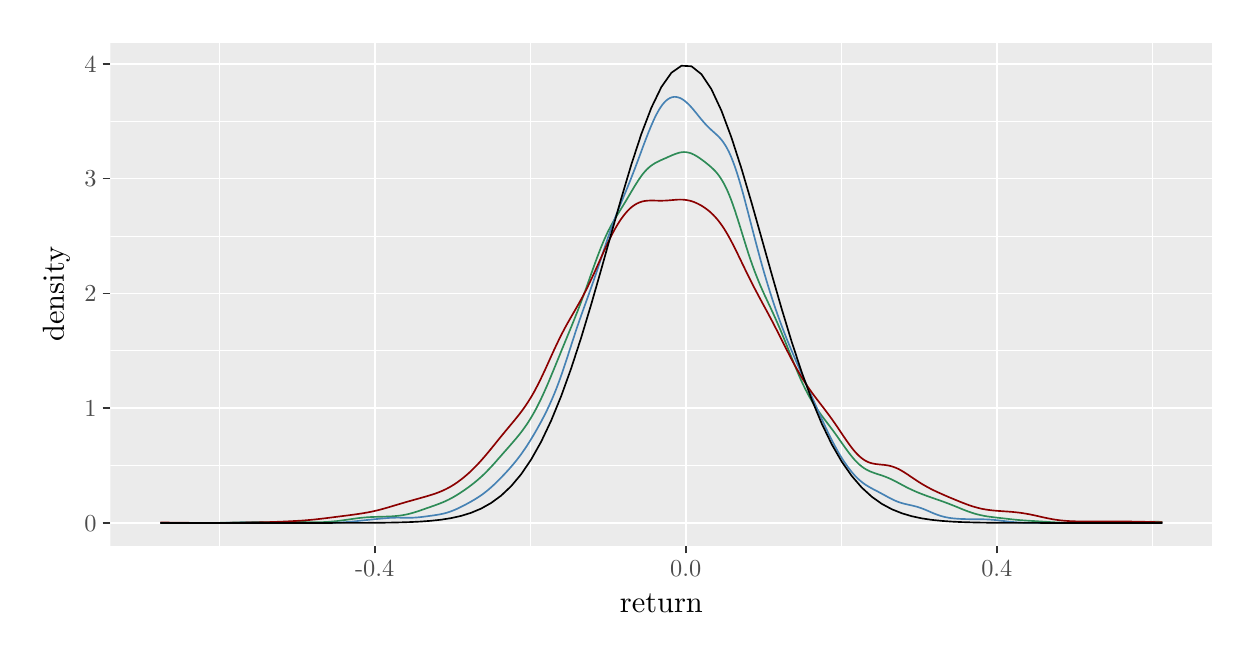
\begin{tikzpicture}[x=1pt,y=1pt]
\definecolor{fillColor}{RGB}{255,255,255}
\path[use as bounding box,fill=fillColor,fill opacity=0.00] (0,0) rectangle (433.62,216.81);
\begin{scope}
\path[clip] (  0.00,  0.00) rectangle (433.62,216.81);
\definecolor{drawColor}{RGB}{255,255,255}
\definecolor{fillColor}{RGB}{255,255,255}

\path[draw=drawColor,line width= 0.6pt,line join=round,line cap=round,fill=fillColor] (  0.00,  0.00) rectangle (433.62,216.81);
\end{scope}
\begin{scope}
\path[clip] ( 29.87, 29.59) rectangle (428.12,211.31);
\definecolor{fillColor}{gray}{0.92}

\path[fill=fillColor] ( 29.87, 29.59) rectangle (428.12,211.31);
\definecolor{drawColor}{RGB}{255,255,255}

\path[draw=drawColor,line width= 0.3pt,line join=round] ( 29.87, 58.58) --
	(428.12, 58.58);

\path[draw=drawColor,line width= 0.3pt,line join=round] ( 29.87,100.06) --
	(428.12,100.06);

\path[draw=drawColor,line width= 0.3pt,line join=round] ( 29.87,141.53) --
	(428.12,141.53);

\path[draw=drawColor,line width= 0.3pt,line join=round] ( 29.87,183.01) --
	(428.12,183.01);

\path[draw=drawColor,line width= 0.3pt,line join=round] ( 69.21, 29.59) --
	( 69.21,211.31);

\path[draw=drawColor,line width= 0.3pt,line join=round] (181.61, 29.59) --
	(181.61,211.31);

\path[draw=drawColor,line width= 0.3pt,line join=round] (294.01, 29.59) --
	(294.01,211.31);

\path[draw=drawColor,line width= 0.3pt,line join=round] (406.41, 29.59) --
	(406.41,211.31);

\path[draw=drawColor,line width= 0.6pt,line join=round] ( 29.87, 37.85) --
	(428.12, 37.85);

\path[draw=drawColor,line width= 0.6pt,line join=round] ( 29.87, 79.32) --
	(428.12, 79.32);

\path[draw=drawColor,line width= 0.6pt,line join=round] ( 29.87,120.80) --
	(428.12,120.80);

\path[draw=drawColor,line width= 0.6pt,line join=round] ( 29.87,162.27) --
	(428.12,162.27);

\path[draw=drawColor,line width= 0.6pt,line join=round] ( 29.87,203.75) --
	(428.12,203.75);

\path[draw=drawColor,line width= 0.6pt,line join=round] (125.41, 29.59) --
	(125.41,211.31);

\path[draw=drawColor,line width= 0.6pt,line join=round] (237.81, 29.59) --
	(237.81,211.31);

\path[draw=drawColor,line width= 0.6pt,line join=round] (350.21, 29.59) --
	(350.21,211.31);
\definecolor{drawColor}{RGB}{46,139,87}

\path[draw=drawColor,line width= 0.6pt,line join=round] ( 47.97, 37.85) --
	( 48.68, 37.85) --
	( 49.39, 37.85) --
	( 50.10, 37.85) --
	( 50.81, 37.85) --
	( 51.51, 37.85) --
	( 52.22, 37.85) --
	( 52.93, 37.85) --
	( 53.64, 37.85) --
	( 54.35, 37.85) --
	( 55.06, 37.85) --
	( 55.76, 37.85) --
	( 56.47, 37.85) --
	( 57.18, 37.85) --
	( 57.89, 37.85) --
	( 58.60, 37.85) --
	( 59.31, 37.85) --
	( 60.02, 37.85) --
	( 60.72, 37.85) --
	( 61.43, 37.85) --
	( 62.14, 37.85) --
	( 62.85, 37.85) --
	( 63.56, 37.85) --
	( 64.27, 37.85) --
	( 64.98, 37.85) --
	( 65.68, 37.85) --
	( 66.39, 37.86) --
	( 67.10, 37.86) --
	( 67.81, 37.86) --
	( 68.52, 37.87) --
	( 69.23, 37.88) --
	( 69.93, 37.89) --
	( 70.64, 37.90) --
	( 71.35, 37.91) --
	( 72.06, 37.92) --
	( 72.77, 37.94) --
	( 73.48, 37.96) --
	( 74.19, 37.98) --
	( 74.89, 38.00) --
	( 75.60, 38.02) --
	( 76.31, 38.05) --
	( 77.02, 38.07) --
	( 77.73, 38.09) --
	( 78.44, 38.11) --
	( 79.15, 38.13) --
	( 79.85, 38.14) --
	( 80.56, 38.15) --
	( 81.27, 38.16) --
	( 81.98, 38.17) --
	( 82.69, 38.17) --
	( 83.40, 38.17) --
	( 84.10, 38.16) --
	( 84.81, 38.16) --
	( 85.52, 38.15) --
	( 86.23, 38.14) --
	( 86.94, 38.13) --
	( 87.65, 38.12) --
	( 88.36, 38.12) --
	( 89.06, 38.12) --
	( 89.77, 38.12) --
	( 90.48, 38.12) --
	( 91.19, 38.13) --
	( 91.90, 38.14) --
	( 92.61, 38.15) --
	( 93.32, 38.16) --
	( 94.02, 38.17) --
	( 94.73, 38.18) --
	( 95.44, 38.19) --
	( 96.15, 38.19) --
	( 96.86, 38.19) --
	( 97.57, 38.19) --
	( 98.28, 38.19) --
	( 98.98, 38.18) --
	( 99.69, 38.17) --
	(100.40, 38.16) --
	(101.11, 38.14) --
	(101.82, 38.13) --
	(102.53, 38.12) --
	(103.23, 38.11) --
	(103.94, 38.11) --
	(104.65, 38.11) --
	(105.36, 38.12) --
	(106.07, 38.13) --
	(106.78, 38.15) --
	(107.49, 38.18) --
	(108.19, 38.22) --
	(108.90, 38.26) --
	(109.61, 38.32) --
	(110.32, 38.38) --
	(111.03, 38.45) --
	(111.74, 38.52) --
	(112.45, 38.61) --
	(113.15, 38.70) --
	(113.86, 38.79) --
	(114.57, 38.89) --
	(115.28, 38.99) --
	(115.99, 39.10) --
	(116.70, 39.20) --
	(117.40, 39.30) --
	(118.11, 39.40) --
	(118.82, 39.50) --
	(119.53, 39.59) --
	(120.24, 39.67) --
	(120.95, 39.74) --
	(121.66, 39.81) --
	(122.36, 39.87) --
	(123.07, 39.92) --
	(123.78, 39.96) --
	(124.49, 39.99) --
	(125.20, 40.02) --
	(125.91, 40.04) --
	(126.62, 40.06) --
	(127.32, 40.08) --
	(128.03, 40.10) --
	(128.74, 40.12) --
	(129.45, 40.14) --
	(130.16, 40.16) --
	(130.87, 40.20) --
	(131.57, 40.23) --
	(132.28, 40.28) --
	(132.99, 40.34) --
	(133.70, 40.41) --
	(134.41, 40.49) --
	(135.12, 40.59) --
	(135.83, 40.71) --
	(136.53, 40.84) --
	(137.24, 40.99) --
	(137.95, 41.16) --
	(138.66, 41.35) --
	(139.37, 41.55) --
	(140.08, 41.77) --
	(140.79, 41.99) --
	(141.49, 42.23) --
	(142.20, 42.47) --
	(142.91, 42.72) --
	(143.62, 42.97) --
	(144.33, 43.22) --
	(145.04, 43.46) --
	(145.74, 43.71) --
	(146.45, 43.96) --
	(147.16, 44.21) --
	(147.87, 44.47) --
	(148.58, 44.73) --
	(149.29, 45.01) --
	(150.00, 45.30) --
	(150.70, 45.60) --
	(151.41, 45.93) --
	(152.12, 46.27) --
	(152.83, 46.64) --
	(153.54, 47.02) --
	(154.25, 47.43) --
	(154.96, 47.85) --
	(155.66, 48.29) --
	(156.37, 48.74) --
	(157.08, 49.21) --
	(157.79, 49.70) --
	(158.50, 50.20) --
	(159.21, 50.71) --
	(159.92, 51.23) --
	(160.62, 51.77) --
	(161.33, 52.33) --
	(162.04, 52.91) --
	(162.75, 53.51) --
	(163.46, 54.13) --
	(164.17, 54.77) --
	(164.87, 55.44) --
	(165.58, 56.14) --
	(166.29, 56.87) --
	(167.00, 57.61) --
	(167.71, 58.37) --
	(168.42, 59.15) --
	(169.13, 59.94) --
	(169.83, 60.75) --
	(170.54, 61.55) --
	(171.25, 62.36) --
	(171.96, 63.17) --
	(172.67, 63.97) --
	(173.38, 64.78) --
	(174.09, 65.58) --
	(174.79, 66.39) --
	(175.50, 67.21) --
	(176.21, 68.04) --
	(176.92, 68.89) --
	(177.63, 69.76) --
	(178.34, 70.66) --
	(179.04, 71.61) --
	(179.75, 72.59) --
	(180.46, 73.63) --
	(181.17, 74.71) --
	(181.88, 75.86) --
	(182.59, 77.06) --
	(183.30, 78.32) --
	(184.00, 79.65) --
	(184.71, 81.05) --
	(185.42, 82.50) --
	(186.13, 84.02) --
	(186.84, 85.58) --
	(187.55, 87.19) --
	(188.26, 88.84) --
	(188.96, 90.53) --
	(189.67, 92.24) --
	(190.38, 93.96) --
	(191.09, 95.70) --
	(191.80, 97.44) --
	(192.51, 99.17) --
	(193.21,100.90) --
	(193.92,102.63) --
	(194.63,104.35) --
	(195.34,106.07) --
	(196.05,107.79) --
	(196.76,109.52) --
	(197.47,111.27) --
	(198.17,113.04) --
	(198.88,114.84) --
	(199.59,116.69) --
	(200.30,118.56) --
	(201.01,120.48) --
	(201.72,122.43) --
	(202.43,124.41) --
	(203.13,126.42) --
	(203.84,128.42) --
	(204.55,130.42) --
	(205.26,132.38) --
	(205.97,134.30) --
	(206.68,136.15) --
	(207.39,137.94) --
	(208.09,139.63) --
	(208.80,141.24) --
	(209.51,142.75) --
	(210.22,144.16) --
	(210.93,145.49) --
	(211.64,146.75) --
	(212.34,147.96) --
	(213.05,149.13) --
	(213.76,150.28) --
	(214.47,151.43) --
	(215.18,152.58) --
	(215.89,153.75) --
	(216.60,154.93) --
	(217.30,156.13) --
	(218.01,157.33) --
	(218.72,158.53) --
	(219.43,159.70) --
	(220.14,160.84) --
	(220.85,161.93) --
	(221.56,162.96) --
	(222.26,163.91) --
	(222.97,164.76) --
	(223.68,165.52) --
	(224.39,166.20) --
	(225.10,166.79) --
	(225.81,167.30) --
	(226.51,167.75) --
	(227.22,168.15) --
	(227.93,168.50) --
	(228.64,168.84) --
	(229.35,169.16) --
	(230.06,169.47) --
	(230.77,169.78) --
	(231.47,170.10) --
	(232.18,170.41) --
	(232.89,170.72) --
	(233.60,171.01) --
	(234.31,171.28) --
	(235.02,171.51) --
	(235.73,171.70) --
	(236.43,171.81) --
	(237.14,171.86) --
	(237.85,171.83) --
	(238.56,171.72) --
	(239.27,171.54) --
	(239.98,171.29) --
	(240.68,170.96) --
	(241.39,170.58) --
	(242.10,170.14) --
	(242.81,169.67) --
	(243.52,169.16) --
	(244.23,168.64) --
	(244.94,168.09) --
	(245.64,167.53) --
	(246.35,166.94) --
	(247.06,166.32) --
	(247.77,165.65) --
	(248.48,164.93) --
	(249.19,164.11) --
	(249.90,163.19) --
	(250.60,162.14) --
	(251.31,160.96) --
	(252.02,159.63) --
	(252.73,158.15) --
	(253.44,156.51) --
	(254.15,154.72) --
	(254.85,152.78) --
	(255.56,150.71) --
	(256.27,148.54) --
	(256.98,146.30) --
	(257.69,144.02) --
	(258.40,141.71) --
	(259.11,139.42) --
	(259.81,137.17) --
	(260.52,134.97) --
	(261.23,132.84) --
	(261.94,130.81) --
	(262.65,128.88) --
	(263.36,127.03) --
	(264.07,125.27) --
	(264.77,123.59) --
	(265.48,121.97) --
	(266.19,120.40) --
	(266.90,118.87) --
	(267.61,117.35) --
	(268.32,115.84) --
	(269.03,114.31) --
	(269.73,112.76) --
	(270.44,111.18) --
	(271.15,109.56) --
	(271.86,107.91) --
	(272.57,106.22) --
	(273.28,104.49) --
	(273.98,102.74) --
	(274.69,100.97) --
	(275.40, 99.20) --
	(276.11, 97.43) --
	(276.82, 95.67) --
	(277.53, 93.95) --
	(278.24, 92.26) --
	(278.94, 90.62) --
	(279.65, 89.04) --
	(280.36, 87.52) --
	(281.07, 86.07) --
	(281.78, 84.70) --
	(282.49, 83.40) --
	(283.20, 82.17) --
	(283.90, 81.01) --
	(284.61, 79.91) --
	(285.32, 78.85) --
	(286.03, 77.85) --
	(286.74, 76.87) --
	(287.45, 75.93) --
	(288.15, 74.99) --
	(288.86, 74.06) --
	(289.57, 73.13) --
	(290.28, 72.19) --
	(290.99, 71.23) --
	(291.70, 70.26) --
	(292.41, 69.27) --
	(293.11, 68.27) --
	(293.82, 67.26) --
	(294.53, 66.25) --
	(295.24, 65.25) --
	(295.95, 64.27) --
	(296.66, 63.31) --
	(297.37, 62.39) --
	(298.07, 61.52) --
	(298.78, 60.69) --
	(299.49, 59.93) --
	(300.20, 59.24) --
	(300.91, 58.62) --
	(301.62, 58.07) --
	(302.32, 57.58) --
	(303.03, 57.15) --
	(303.74, 56.78) --
	(304.45, 56.45) --
	(305.16, 56.17) --
	(305.87, 55.91) --
	(306.58, 55.67) --
	(307.28, 55.44) --
	(307.99, 55.21) --
	(308.70, 54.98) --
	(309.41, 54.73) --
	(310.12, 54.46) --
	(310.83, 54.17) --
	(311.54, 53.86) --
	(312.24, 53.53) --
	(312.95, 53.18) --
	(313.66, 52.82) --
	(314.37, 52.45) --
	(315.08, 52.07) --
	(315.79, 51.69) --
	(316.49, 51.31) --
	(317.20, 50.94) --
	(317.91, 50.58) --
	(318.62, 50.23) --
	(319.33, 49.89) --
	(320.04, 49.57) --
	(320.75, 49.25) --
	(321.45, 48.95) --
	(322.16, 48.66) --
	(322.87, 48.38) --
	(323.58, 48.11) --
	(324.29, 47.84) --
	(325.00, 47.58) --
	(325.71, 47.33) --
	(326.41, 47.08) --
	(327.12, 46.83) --
	(327.83, 46.58) --
	(328.54, 46.34) --
	(329.25, 46.09) --
	(329.96, 45.84) --
	(330.67, 45.59) --
	(331.37, 45.33) --
	(332.08, 45.07) --
	(332.79, 44.80) --
	(333.50, 44.52) --
	(334.21, 44.24) --
	(334.92, 43.96) --
	(335.62, 43.67) --
	(336.33, 43.38) --
	(337.04, 43.09) --
	(337.75, 42.80) --
	(338.46, 42.52) --
	(339.17, 42.24) --
	(339.88, 41.98) --
	(340.58, 41.73) --
	(341.29, 41.49) --
	(342.00, 41.27) --
	(342.71, 41.06) --
	(343.42, 40.88) --
	(344.13, 40.71) --
	(344.84, 40.55) --
	(345.54, 40.42) --
	(346.25, 40.29) --
	(346.96, 40.18) --
	(347.67, 40.08) --
	(348.38, 39.99) --
	(349.09, 39.90) --
	(349.79, 39.82) --
	(350.50, 39.73) --
	(351.21, 39.65) --
	(351.92, 39.57) --
	(352.63, 39.49) --
	(353.34, 39.41) --
	(354.05, 39.33) --
	(354.75, 39.25) --
	(355.46, 39.17) --
	(356.17, 39.09) --
	(356.88, 39.02) --
	(357.59, 38.95) --
	(358.30, 38.89) --
	(359.01, 38.83) --
	(359.71, 38.78) --
	(360.42, 38.73) --
	(361.13, 38.68) --
	(361.84, 38.64) --
	(362.55, 38.59) --
	(363.26, 38.55) --
	(363.96, 38.51) --
	(364.67, 38.47) --
	(365.38, 38.42) --
	(366.09, 38.38) --
	(366.80, 38.33) --
	(367.51, 38.29) --
	(368.22, 38.24) --
	(368.92, 38.19) --
	(369.63, 38.15) --
	(370.34, 38.11) --
	(371.05, 38.07) --
	(371.76, 38.03) --
	(372.47, 38.00) --
	(373.18, 37.97) --
	(373.88, 37.95) --
	(374.59, 37.92) --
	(375.30, 37.91) --
	(376.01, 37.89) --
	(376.72, 37.88) --
	(377.43, 37.87) --
	(378.13, 37.87) --
	(378.84, 37.86) --
	(379.55, 37.86) --
	(380.26, 37.85) --
	(380.97, 37.85) --
	(381.68, 37.85) --
	(382.39, 37.85) --
	(383.09, 37.85) --
	(383.80, 37.85) --
	(384.51, 37.85) --
	(385.22, 37.85) --
	(385.93, 37.85) --
	(386.64, 37.85) --
	(387.35, 37.85) --
	(388.05, 37.86) --
	(388.76, 37.86) --
	(389.47, 37.86) --
	(390.18, 37.87) --
	(390.89, 37.88) --
	(391.60, 37.88) --
	(392.31, 37.89) --
	(393.01, 37.91) --
	(393.72, 37.92) --
	(394.43, 37.93) --
	(395.14, 37.95) --
	(395.85, 37.97) --
	(396.56, 37.99) --
	(397.26, 38.01) --
	(397.97, 38.03) --
	(398.68, 38.05) --
	(399.39, 38.08) --
	(400.10, 38.10) --
	(400.81, 38.12) --
	(401.52, 38.15) --
	(402.22, 38.17) --
	(402.93, 38.19) --
	(403.64, 38.21) --
	(404.35, 38.22) --
	(405.06, 38.24) --
	(405.77, 38.25) --
	(406.48, 38.25) --
	(407.18, 38.26) --
	(407.89, 38.25) --
	(408.60, 38.25) --
	(409.31, 38.24) --
	(410.02, 38.22);
\definecolor{drawColor}{RGB}{70,130,180}

\path[draw=drawColor,line width= 0.6pt,line join=round] ( 47.97, 37.85) --
	( 48.68, 37.85) --
	( 49.39, 37.85) --
	( 50.10, 37.85) --
	( 50.81, 37.85) --
	( 51.51, 37.85) --
	( 52.22, 37.85) --
	( 52.93, 37.85) --
	( 53.64, 37.85) --
	( 54.35, 37.85) --
	( 55.06, 37.85) --
	( 55.76, 37.85) --
	( 56.47, 37.85) --
	( 57.18, 37.85) --
	( 57.89, 37.85) --
	( 58.60, 37.85) --
	( 59.31, 37.85) --
	( 60.02, 37.85) --
	( 60.72, 37.85) --
	( 61.43, 37.85) --
	( 62.14, 37.85) --
	( 62.85, 37.85) --
	( 63.56, 37.85) --
	( 64.27, 37.85) --
	( 64.98, 37.85) --
	( 65.68, 37.85) --
	( 66.39, 37.85) --
	( 67.10, 37.85) --
	( 67.81, 37.85) --
	( 68.52, 37.86) --
	( 69.23, 37.86) --
	( 69.93, 37.86) --
	( 70.64, 37.87) --
	( 71.35, 37.88) --
	( 72.06, 37.89) --
	( 72.77, 37.90) --
	( 73.48, 37.91) --
	( 74.19, 37.93) --
	( 74.89, 37.94) --
	( 75.60, 37.96) --
	( 76.31, 37.97) --
	( 77.02, 37.99) --
	( 77.73, 38.00) --
	( 78.44, 38.02) --
	( 79.15, 38.02) --
	( 79.85, 38.03) --
	( 80.56, 38.03) --
	( 81.27, 38.03) --
	( 81.98, 38.03) --
	( 82.69, 38.02) --
	( 83.40, 38.01) --
	( 84.10, 38.00) --
	( 84.81, 37.98) --
	( 85.52, 37.96) --
	( 86.23, 37.95) --
	( 86.94, 37.93) --
	( 87.65, 37.92) --
	( 88.36, 37.90) --
	( 89.06, 37.89) --
	( 89.77, 37.88) --
	( 90.48, 37.87) --
	( 91.19, 37.87) --
	( 91.90, 37.86) --
	( 92.61, 37.86) --
	( 93.32, 37.85) --
	( 94.02, 37.85) --
	( 94.73, 37.85) --
	( 95.44, 37.85) --
	( 96.15, 37.85) --
	( 96.86, 37.85) --
	( 97.57, 37.85) --
	( 98.28, 37.85) --
	( 98.98, 37.85) --
	( 99.69, 37.85) --
	(100.40, 37.85) --
	(101.11, 37.85) --
	(101.82, 37.85) --
	(102.53, 37.85) --
	(103.23, 37.85) --
	(103.94, 37.85) --
	(104.65, 37.85) --
	(105.36, 37.85) --
	(106.07, 37.85) --
	(106.78, 37.86) --
	(107.49, 37.86) --
	(108.19, 37.87) --
	(108.90, 37.88) --
	(109.61, 37.89) --
	(110.32, 37.91) --
	(111.03, 37.93) --
	(111.74, 37.96) --
	(112.45, 37.99) --
	(113.15, 38.02) --
	(113.86, 38.06) --
	(114.57, 38.11) --
	(115.28, 38.17) --
	(115.99, 38.23) --
	(116.70, 38.29) --
	(117.40, 38.36) --
	(118.11, 38.43) --
	(118.82, 38.50) --
	(119.53, 38.58) --
	(120.24, 38.66) --
	(120.95, 38.73) --
	(121.66, 38.81) --
	(122.36, 38.88) --
	(123.07, 38.95) --
	(123.78, 39.03) --
	(124.49, 39.10) --
	(125.20, 39.17) --
	(125.91, 39.24) --
	(126.62, 39.31) --
	(127.32, 39.38) --
	(128.03, 39.44) --
	(128.74, 39.51) --
	(129.45, 39.57) --
	(130.16, 39.62) --
	(130.87, 39.67) --
	(131.57, 39.70) --
	(132.28, 39.73) --
	(132.99, 39.75) --
	(133.70, 39.75) --
	(134.41, 39.75) --
	(135.12, 39.74) --
	(135.83, 39.73) --
	(136.53, 39.72) --
	(137.24, 39.71) --
	(137.95, 39.71) --
	(138.66, 39.73) --
	(139.37, 39.75) --
	(140.08, 39.79) --
	(140.79, 39.84) --
	(141.49, 39.91) --
	(142.20, 39.98) --
	(142.91, 40.07) --
	(143.62, 40.16) --
	(144.33, 40.25) --
	(145.04, 40.35) --
	(145.74, 40.45) --
	(146.45, 40.54) --
	(147.16, 40.65) --
	(147.87, 40.76) --
	(148.58, 40.88) --
	(149.29, 41.01) --
	(150.00, 41.16) --
	(150.70, 41.33) --
	(151.41, 41.53) --
	(152.12, 41.74) --
	(152.83, 41.99) --
	(153.54, 42.26) --
	(154.25, 42.55) --
	(154.96, 42.86) --
	(155.66, 43.19) --
	(156.37, 43.53) --
	(157.08, 43.89) --
	(157.79, 44.25) --
	(158.50, 44.63) --
	(159.21, 45.01) --
	(159.92, 45.40) --
	(160.62, 45.81) --
	(161.33, 46.22) --
	(162.04, 46.65) --
	(162.75, 47.10) --
	(163.46, 47.57) --
	(164.17, 48.06) --
	(164.87, 48.58) --
	(165.58, 49.13) --
	(166.29, 49.70) --
	(167.00, 50.31) --
	(167.71, 50.94) --
	(168.42, 51.59) --
	(169.13, 52.27) --
	(169.83, 52.96) --
	(170.54, 53.67) --
	(171.25, 54.40) --
	(171.96, 55.14) --
	(172.67, 55.89) --
	(173.38, 56.66) --
	(174.09, 57.45) --
	(174.79, 58.26) --
	(175.50, 59.09) --
	(176.21, 59.95) --
	(176.92, 60.84) --
	(177.63, 61.76) --
	(178.34, 62.72) --
	(179.04, 63.72) --
	(179.75, 64.75) --
	(180.46, 65.82) --
	(181.17, 66.93) --
	(181.88, 68.07) --
	(182.59, 69.24) --
	(183.30, 70.44) --
	(184.00, 71.67) --
	(184.71, 72.94) --
	(185.42, 74.23) --
	(186.13, 75.57) --
	(186.84, 76.95) --
	(187.55, 78.38) --
	(188.26, 79.87) --
	(188.96, 81.42) --
	(189.67, 83.03) --
	(190.38, 84.73) --
	(191.09, 86.51) --
	(191.80, 88.37) --
	(192.51, 90.32) --
	(193.21, 92.34) --
	(193.92, 94.44) --
	(194.63, 96.59) --
	(195.34, 98.77) --
	(196.05,100.96) --
	(196.76,103.15) --
	(197.47,105.33) --
	(198.17,107.47) --
	(198.88,109.57) --
	(199.59,111.62) --
	(200.30,113.64) --
	(201.01,115.62) --
	(201.72,117.58) --
	(202.43,119.55) --
	(203.13,121.52) --
	(203.84,123.52) --
	(204.55,125.55) --
	(205.26,127.62) --
	(205.97,129.72) --
	(206.68,131.86) --
	(207.39,134.01) --
	(208.09,136.16) --
	(208.80,138.30) --
	(209.51,140.41) --
	(210.22,142.47) --
	(210.93,144.47) --
	(211.64,146.42) --
	(212.34,148.30) --
	(213.05,150.12) --
	(213.76,151.89) --
	(214.47,153.62) --
	(215.18,155.34) --
	(215.89,157.05) --
	(216.60,158.77) --
	(217.30,160.52) --
	(218.01,162.29) --
	(218.72,164.11) --
	(219.43,165.95) --
	(220.14,167.83) --
	(220.85,169.74) --
	(221.56,171.65) --
	(222.26,173.57) --
	(222.97,175.46) --
	(223.68,177.32) --
	(224.39,179.13) --
	(225.10,180.86) --
	(225.81,182.51) --
	(226.51,184.06) --
	(227.22,185.49) --
	(227.93,186.79) --
	(228.64,187.96) --
	(229.35,188.96) --
	(230.06,189.81) --
	(230.77,190.50) --
	(231.47,191.04) --
	(232.18,191.43) --
	(232.89,191.68) --
	(233.60,191.80) --
	(234.31,191.78) --
	(235.02,191.64) --
	(235.73,191.39) --
	(236.43,191.03) --
	(237.14,190.56) --
	(237.85,190.00) --
	(238.56,189.35) --
	(239.27,188.64) --
	(239.98,187.86) --
	(240.68,187.04) --
	(241.39,186.18) --
	(242.10,185.30) --
	(242.81,184.42) --
	(243.52,183.55) --
	(244.23,182.72) --
	(244.94,181.93) --
	(245.64,181.19) --
	(246.35,180.49) --
	(247.06,179.83) --
	(247.77,179.19) --
	(248.48,178.55) --
	(249.19,177.90) --
	(249.90,177.19) --
	(250.60,176.40) --
	(251.31,175.49) --
	(252.02,174.43) --
	(252.73,173.21) --
	(253.44,171.82) --
	(254.15,170.24) --
	(254.85,168.48) --
	(255.56,166.54) --
	(256.27,164.42) --
	(256.98,162.16) --
	(257.69,159.75) --
	(258.40,157.22) --
	(259.11,154.60) --
	(259.81,151.92) --
	(260.52,149.20) --
	(261.23,146.46) --
	(261.94,143.72) --
	(262.65,140.99) --
	(263.36,138.30) --
	(264.07,135.65) --
	(264.77,133.05) --
	(265.48,130.51) --
	(266.19,128.04) --
	(266.90,125.64) --
	(267.61,123.30) --
	(268.32,121.04) --
	(269.03,118.84) --
	(269.73,116.70) --
	(270.44,114.63) --
	(271.15,112.61) --
	(271.86,110.66) --
	(272.57,108.76) --
	(273.28,106.91) --
	(273.98,105.11) --
	(274.69,103.35) --
	(275.40,101.63) --
	(276.11, 99.94) --
	(276.82, 98.27) --
	(277.53, 96.63) --
	(278.24, 95.00) --
	(278.94, 93.39) --
	(279.65, 91.80) --
	(280.36, 90.20) --
	(281.07, 88.61) --
	(281.78, 87.02) --
	(282.49, 85.43) --
	(283.20, 83.83) --
	(283.90, 82.24) --
	(284.61, 80.64) --
	(285.32, 79.04) --
	(286.03, 77.44) --
	(286.74, 75.86) --
	(287.45, 74.30) --
	(288.15, 72.76) --
	(288.86, 71.25) --
	(289.57, 69.78) --
	(290.28, 68.35) --
	(290.99, 66.96) --
	(291.70, 65.62) --
	(292.41, 64.32) --
	(293.11, 63.08) --
	(293.82, 61.89) --
	(294.53, 60.76) --
	(295.24, 59.68) --
	(295.95, 58.65) --
	(296.66, 57.68) --
	(297.37, 56.76) --
	(298.07, 55.90) --
	(298.78, 55.10) --
	(299.49, 54.35) --
	(300.20, 53.67) --
	(300.91, 53.04) --
	(301.62, 52.47) --
	(302.32, 51.95) --
	(303.03, 51.47) --
	(303.74, 51.04) --
	(304.45, 50.63) --
	(305.16, 50.24) --
	(305.87, 49.86) --
	(306.58, 49.49) --
	(307.28, 49.13) --
	(307.99, 48.75) --
	(308.70, 48.37) --
	(309.41, 47.99) --
	(310.12, 47.60) --
	(310.83, 47.21) --
	(311.54, 46.84) --
	(312.24, 46.47) --
	(312.95, 46.13) --
	(313.66, 45.81) --
	(314.37, 45.52) --
	(315.08, 45.27) --
	(315.79, 45.04) --
	(316.49, 44.85) --
	(317.20, 44.67) --
	(317.91, 44.51) --
	(318.62, 44.35) --
	(319.33, 44.20) --
	(320.04, 44.03) --
	(320.75, 43.85) --
	(321.45, 43.66) --
	(322.16, 43.43) --
	(322.87, 43.19) --
	(323.58, 42.92) --
	(324.29, 42.63) --
	(325.00, 42.34) --
	(325.71, 42.03) --
	(326.41, 41.72) --
	(327.12, 41.42) --
	(327.83, 41.13) --
	(328.54, 40.86) --
	(329.25, 40.61) --
	(329.96, 40.38) --
	(330.67, 40.18) --
	(331.37, 40.00) --
	(332.08, 39.85) --
	(332.79, 39.72) --
	(333.50, 39.61) --
	(334.21, 39.52) --
	(334.92, 39.45) --
	(335.62, 39.39) --
	(336.33, 39.34) --
	(337.04, 39.30) --
	(337.75, 39.27) --
	(338.46, 39.25) --
	(339.17, 39.23) --
	(339.88, 39.21) --
	(340.58, 39.20) --
	(341.29, 39.19) --
	(342.00, 39.19) --
	(342.71, 39.19) --
	(343.42, 39.18) --
	(344.13, 39.18) --
	(344.84, 39.17) --
	(345.54, 39.15) --
	(346.25, 39.13) --
	(346.96, 39.10) --
	(347.67, 39.06) --
	(348.38, 39.01) --
	(349.09, 38.95) --
	(349.79, 38.88) --
	(350.50, 38.81) --
	(351.21, 38.73) --
	(351.92, 38.64) --
	(352.63, 38.56) --
	(353.34, 38.47) --
	(354.05, 38.39) --
	(354.75, 38.31) --
	(355.46, 38.23) --
	(356.17, 38.17) --
	(356.88, 38.11) --
	(357.59, 38.05) --
	(358.30, 38.01) --
	(359.01, 37.97) --
	(359.71, 37.94) --
	(360.42, 37.92) --
	(361.13, 37.90) --
	(361.84, 37.89) --
	(362.55, 37.87) --
	(363.26, 37.87) --
	(363.96, 37.86) --
	(364.67, 37.86) --
	(365.38, 37.85) --
	(366.09, 37.85) --
	(366.80, 37.85) --
	(367.51, 37.85) --
	(368.22, 37.85) --
	(368.92, 37.85) --
	(369.63, 37.85) --
	(370.34, 37.85) --
	(371.05, 37.85) --
	(371.76, 37.85) --
	(372.47, 37.85) --
	(373.18, 37.85) --
	(373.88, 37.85) --
	(374.59, 37.85) --
	(375.30, 37.85) --
	(376.01, 37.85) --
	(376.72, 37.86) --
	(377.43, 37.86) --
	(378.13, 37.86) --
	(378.84, 37.87) --
	(379.55, 37.88) --
	(380.26, 37.88) --
	(380.97, 37.90) --
	(381.68, 37.91) --
	(382.39, 37.92) --
	(383.09, 37.94) --
	(383.80, 37.95) --
	(384.51, 37.97) --
	(385.22, 37.98) --
	(385.93, 38.00) --
	(386.64, 38.01) --
	(387.35, 38.02) --
	(388.05, 38.03) --
	(388.76, 38.03) --
	(389.47, 38.03) --
	(390.18, 38.03) --
	(390.89, 38.02) --
	(391.60, 38.01) --
	(392.31, 38.00) --
	(393.01, 37.99) --
	(393.72, 37.97) --
	(394.43, 37.95) --
	(395.14, 37.94) --
	(395.85, 37.92) --
	(396.56, 37.91) --
	(397.26, 37.90) --
	(397.97, 37.89) --
	(398.68, 37.88) --
	(399.39, 37.87) --
	(400.10, 37.86) --
	(400.81, 37.86) --
	(401.52, 37.86) --
	(402.22, 37.85) --
	(402.93, 37.85) --
	(403.64, 37.85) --
	(404.35, 37.85) --
	(405.06, 37.85) --
	(405.77, 37.85) --
	(406.48, 37.85) --
	(407.18, 37.85) --
	(407.89, 37.85) --
	(408.60, 37.85) --
	(409.31, 37.85) --
	(410.02, 37.85);
\definecolor{drawColor}{RGB}{139,0,0}

\path[draw=drawColor,line width= 0.6pt,line join=round] ( 47.97, 37.99) --
	( 48.68, 37.99) --
	( 49.39, 37.99) --
	( 50.10, 37.99) --
	( 50.81, 37.98) --
	( 51.51, 37.97) --
	( 52.22, 37.96) --
	( 52.93, 37.95) --
	( 53.64, 37.95) --
	( 54.35, 37.94) --
	( 55.06, 37.93) --
	( 55.76, 37.92) --
	( 56.47, 37.91) --
	( 57.18, 37.90) --
	( 57.89, 37.89) --
	( 58.60, 37.88) --
	( 59.31, 37.88) --
	( 60.02, 37.87) --
	( 60.72, 37.87) --
	( 61.43, 37.86) --
	( 62.14, 37.86) --
	( 62.85, 37.86) --
	( 63.56, 37.86) --
	( 64.27, 37.85) --
	( 64.98, 37.85) --
	( 65.68, 37.85) --
	( 66.39, 37.85) --
	( 67.10, 37.85) --
	( 67.81, 37.86) --
	( 68.52, 37.86) --
	( 69.23, 37.86) --
	( 69.93, 37.86) --
	( 70.64, 37.87) --
	( 71.35, 37.87) --
	( 72.06, 37.88) --
	( 72.77, 37.88) --
	( 73.48, 37.89) --
	( 74.19, 37.90) --
	( 74.89, 37.91) --
	( 75.60, 37.92) --
	( 76.31, 37.93) --
	( 77.02, 37.94) --
	( 77.73, 37.95) --
	( 78.44, 37.97) --
	( 79.15, 37.98) --
	( 79.85, 37.99) --
	( 80.56, 38.01) --
	( 81.27, 38.02) --
	( 81.98, 38.03) --
	( 82.69, 38.05) --
	( 83.40, 38.06) --
	( 84.10, 38.07) --
	( 84.81, 38.09) --
	( 85.52, 38.11) --
	( 86.23, 38.12) --
	( 86.94, 38.14) --
	( 87.65, 38.16) --
	( 88.36, 38.18) --
	( 89.06, 38.21) --
	( 89.77, 38.23) --
	( 90.48, 38.26) --
	( 91.19, 38.29) --
	( 91.90, 38.32) --
	( 92.61, 38.35) --
	( 93.32, 38.38) --
	( 94.02, 38.42) --
	( 94.73, 38.45) --
	( 95.44, 38.49) --
	( 96.15, 38.53) --
	( 96.86, 38.56) --
	( 97.57, 38.61) --
	( 98.28, 38.65) --
	( 98.98, 38.69) --
	( 99.69, 38.74) --
	(100.40, 38.80) --
	(101.11, 38.85) --
	(101.82, 38.92) --
	(102.53, 38.98) --
	(103.23, 39.05) --
	(103.94, 39.12) --
	(104.65, 39.20) --
	(105.36, 39.28) --
	(106.07, 39.36) --
	(106.78, 39.45) --
	(107.49, 39.53) --
	(108.19, 39.62) --
	(108.90, 39.71) --
	(109.61, 39.80) --
	(110.32, 39.89) --
	(111.03, 39.98) --
	(111.74, 40.07) --
	(112.45, 40.16) --
	(113.15, 40.25) --
	(113.86, 40.34) --
	(114.57, 40.43) --
	(115.28, 40.52) --
	(115.99, 40.61) --
	(116.70, 40.71) --
	(117.40, 40.80) --
	(118.11, 40.90) --
	(118.82, 41.00) --
	(119.53, 41.10) --
	(120.24, 41.21) --
	(120.95, 41.32) --
	(121.66, 41.44) --
	(122.36, 41.56) --
	(123.07, 41.69) --
	(123.78, 41.83) --
	(124.49, 41.97) --
	(125.20, 42.13) --
	(125.91, 42.29) --
	(126.62, 42.46) --
	(127.32, 42.64) --
	(128.03, 42.83) --
	(128.74, 43.03) --
	(129.45, 43.23) --
	(130.16, 43.43) --
	(130.87, 43.64) --
	(131.57, 43.85) --
	(132.28, 44.07) --
	(132.99, 44.28) --
	(133.70, 44.49) --
	(134.41, 44.70) --
	(135.12, 44.91) --
	(135.83, 45.12) --
	(136.53, 45.33) --
	(137.24, 45.53) --
	(137.95, 45.73) --
	(138.66, 45.93) --
	(139.37, 46.13) --
	(140.08, 46.33) --
	(140.79, 46.52) --
	(141.49, 46.72) --
	(142.20, 46.92) --
	(142.91, 47.12) --
	(143.62, 47.32) --
	(144.33, 47.53) --
	(145.04, 47.74) --
	(145.74, 47.96) --
	(146.45, 48.18) --
	(147.16, 48.42) --
	(147.87, 48.67) --
	(148.58, 48.94) --
	(149.29, 49.23) --
	(150.00, 49.53) --
	(150.70, 49.86) --
	(151.41, 50.21) --
	(152.12, 50.58) --
	(152.83, 50.98) --
	(153.54, 51.40) --
	(154.25, 51.85) --
	(154.96, 52.32) --
	(155.66, 52.83) --
	(156.37, 53.35) --
	(157.08, 53.90) --
	(157.79, 54.48) --
	(158.50, 55.08) --
	(159.21, 55.70) --
	(159.92, 56.35) --
	(160.62, 57.03) --
	(161.33, 57.73) --
	(162.04, 58.45) --
	(162.75, 59.19) --
	(163.46, 59.96) --
	(164.17, 60.75) --
	(164.87, 61.56) --
	(165.58, 62.39) --
	(166.29, 63.23) --
	(167.00, 64.09) --
	(167.71, 64.96) --
	(168.42, 65.83) --
	(169.13, 66.71) --
	(169.83, 67.59) --
	(170.54, 68.46) --
	(171.25, 69.33) --
	(171.96, 70.19) --
	(172.67, 71.05) --
	(173.38, 71.90) --
	(174.09, 72.75) --
	(174.79, 73.60) --
	(175.50, 74.45) --
	(176.21, 75.31) --
	(176.92, 76.19) --
	(177.63, 77.08) --
	(178.34, 78.01) --
	(179.04, 78.97) --
	(179.75, 79.97) --
	(180.46, 81.02) --
	(181.17, 82.12) --
	(181.88, 83.27) --
	(182.59, 84.48) --
	(183.30, 85.76) --
	(184.00, 87.10) --
	(184.71, 88.49) --
	(185.42, 89.93) --
	(186.13, 91.42) --
	(186.84, 92.94) --
	(187.55, 94.49) --
	(188.26, 96.05) --
	(188.96, 97.62) --
	(189.67, 99.18) --
	(190.38,100.72) --
	(191.09,102.23) --
	(191.80,103.71) --
	(192.51,105.15) --
	(193.21,106.54) --
	(193.92,107.90) --
	(194.63,109.21) --
	(195.34,110.48) --
	(196.05,111.72) --
	(196.76,112.95) --
	(197.47,114.17) --
	(198.17,115.39) --
	(198.88,116.63) --
	(199.59,117.89) --
	(200.30,119.18) --
	(201.01,120.52) --
	(201.72,121.90) --
	(202.43,123.32) --
	(203.13,124.78) --
	(203.84,126.29) --
	(204.55,127.82) --
	(205.26,129.39) --
	(205.97,130.97) --
	(206.68,132.56) --
	(207.39,134.15) --
	(208.09,135.72) --
	(208.80,137.26) --
	(209.51,138.77) --
	(210.22,140.24) --
	(210.93,141.65) --
	(211.64,143.01) --
	(212.34,144.29) --
	(213.05,145.50) --
	(213.76,146.64) --
	(214.47,147.70) --
	(215.18,148.68) --
	(215.89,149.58) --
	(216.60,150.40) --
	(217.30,151.14) --
	(218.01,151.79) --
	(218.72,152.35) --
	(219.43,152.83) --
	(220.14,153.24) --
	(220.85,153.57) --
	(221.56,153.84) --
	(222.26,154.04) --
	(222.97,154.18) --
	(223.68,154.27) --
	(224.39,154.32) --
	(225.10,154.34) --
	(225.81,154.34) --
	(226.51,154.33) --
	(227.22,154.31) --
	(227.93,154.29) --
	(228.64,154.28) --
	(229.35,154.29) --
	(230.06,154.31) --
	(230.77,154.34) --
	(231.47,154.39) --
	(232.18,154.45) --
	(232.89,154.51) --
	(233.60,154.57) --
	(234.31,154.63) --
	(235.02,154.67) --
	(235.73,154.69) --
	(236.43,154.68) --
	(237.14,154.63) --
	(237.85,154.55) --
	(238.56,154.44) --
	(239.27,154.28) --
	(239.98,154.08) --
	(240.68,153.84) --
	(241.39,153.55) --
	(242.10,153.22) --
	(242.81,152.86) --
	(243.52,152.46) --
	(244.23,152.02) --
	(244.94,151.53) --
	(245.64,151.01) --
	(246.35,150.44) --
	(247.06,149.80) --
	(247.77,149.11) --
	(248.48,148.36) --
	(249.19,147.55) --
	(249.90,146.66) --
	(250.60,145.70) --
	(251.31,144.68) --
	(252.02,143.57) --
	(252.73,142.39) --
	(253.44,141.14) --
	(254.15,139.83) --
	(254.85,138.47) --
	(255.56,137.07) --
	(256.27,135.63) --
	(256.98,134.17) --
	(257.69,132.70) --
	(258.40,131.22) --
	(259.11,129.75) --
	(259.81,128.29) --
	(260.52,126.85) --
	(261.23,125.43) --
	(261.94,124.03) --
	(262.65,122.66) --
	(263.36,121.31) --
	(264.07,119.97) --
	(264.77,118.66) --
	(265.48,117.34) --
	(266.19,116.03) --
	(266.90,114.72) --
	(267.61,113.40) --
	(268.32,112.07) --
	(269.03,110.73) --
	(269.73,109.37) --
	(270.44,107.99) --
	(271.15,106.60) --
	(271.86,105.19) --
	(272.57,103.79) --
	(273.28,102.38) --
	(273.98,100.97) --
	(274.69, 99.57) --
	(275.40, 98.19) --
	(276.11, 96.84) --
	(276.82, 95.51) --
	(277.53, 94.21) --
	(278.24, 92.95) --
	(278.94, 91.73) --
	(279.65, 90.54) --
	(280.36, 89.39) --
	(281.07, 88.29) --
	(281.78, 87.23) --
	(282.49, 86.20) --
	(283.20, 85.20) --
	(283.90, 84.23) --
	(284.61, 83.28) --
	(285.32, 82.35) --
	(286.03, 81.43) --
	(286.74, 80.51) --
	(287.45, 79.59) --
	(288.15, 78.66) --
	(288.86, 77.72) --
	(289.57, 76.77) --
	(290.28, 75.79) --
	(290.99, 74.80) --
	(291.70, 73.79) --
	(292.41, 72.75) --
	(293.11, 71.71) --
	(293.82, 70.65) --
	(294.53, 69.60) --
	(295.24, 68.55) --
	(295.95, 67.52) --
	(296.66, 66.52) --
	(297.37, 65.55) --
	(298.07, 64.63) --
	(298.78, 63.78) --
	(299.49, 62.99) --
	(300.20, 62.27) --
	(300.91, 61.62) --
	(301.62, 61.06) --
	(302.32, 60.57) --
	(303.03, 60.16) --
	(303.74, 59.83) --
	(304.45, 59.57) --
	(305.16, 59.37) --
	(305.87, 59.22) --
	(306.58, 59.11) --
	(307.28, 59.03) --
	(307.99, 58.96) --
	(308.70, 58.89) --
	(309.41, 58.83) --
	(310.12, 58.74) --
	(310.83, 58.62) --
	(311.54, 58.47) --
	(312.24, 58.28) --
	(312.95, 58.05) --
	(313.66, 57.78) --
	(314.37, 57.47) --
	(315.08, 57.11) --
	(315.79, 56.72) --
	(316.49, 56.30) --
	(317.20, 55.85) --
	(317.91, 55.39) --
	(318.62, 54.91) --
	(319.33, 54.43) --
	(320.04, 53.95) --
	(320.75, 53.47) --
	(321.45, 53.00) --
	(322.16, 52.55) --
	(322.87, 52.11) --
	(323.58, 51.68) --
	(324.29, 51.27) --
	(325.00, 50.87) --
	(325.71, 50.49) --
	(326.41, 50.12) --
	(327.12, 49.77) --
	(327.83, 49.42) --
	(328.54, 49.09) --
	(329.25, 48.76) --
	(329.96, 48.45) --
	(330.67, 48.13) --
	(331.37, 47.82) --
	(332.08, 47.52) --
	(332.79, 47.21) --
	(333.50, 46.91) --
	(334.21, 46.62) --
	(334.92, 46.32) --
	(335.62, 46.03) --
	(336.33, 45.74) --
	(337.04, 45.45) --
	(337.75, 45.17) --
	(338.46, 44.90) --
	(339.17, 44.63) --
	(339.88, 44.37) --
	(340.58, 44.13) --
	(341.29, 43.89) --
	(342.00, 43.67) --
	(342.71, 43.47) --
	(343.42, 43.28) --
	(344.13, 43.10) --
	(344.84, 42.95) --
	(345.54, 42.81) --
	(346.25, 42.69) --
	(346.96, 42.58) --
	(347.67, 42.49) --
	(348.38, 42.40) --
	(349.09, 42.33) --
	(349.79, 42.27) --
	(350.50, 42.21) --
	(351.21, 42.16) --
	(351.92, 42.11) --
	(352.63, 42.06) --
	(353.34, 42.01) --
	(354.05, 41.97) --
	(354.75, 41.91) --
	(355.46, 41.86) --
	(356.17, 41.79) --
	(356.88, 41.72) --
	(357.59, 41.64) --
	(358.30, 41.56) --
	(359.01, 41.46) --
	(359.71, 41.36) --
	(360.42, 41.24) --
	(361.13, 41.12) --
	(361.84, 40.99) --
	(362.55, 40.85) --
	(363.26, 40.70) --
	(363.96, 40.55) --
	(364.67, 40.39) --
	(365.38, 40.23) --
	(366.09, 40.07) --
	(366.80, 39.91) --
	(367.51, 39.75) --
	(368.22, 39.60) --
	(368.92, 39.46) --
	(369.63, 39.32) --
	(370.34, 39.19) --
	(371.05, 39.07) --
	(371.76, 38.97) --
	(372.47, 38.87) --
	(373.18, 38.78) --
	(373.88, 38.71) --
	(374.59, 38.64) --
	(375.30, 38.59) --
	(376.01, 38.54) --
	(376.72, 38.50) --
	(377.43, 38.47) --
	(378.13, 38.44) --
	(378.84, 38.42) --
	(379.55, 38.40) --
	(380.26, 38.39) --
	(380.97, 38.38) --
	(381.68, 38.38) --
	(382.39, 38.38) --
	(383.09, 38.38) --
	(383.80, 38.38) --
	(384.51, 38.39) --
	(385.22, 38.39) --
	(385.93, 38.40) --
	(386.64, 38.40) --
	(387.35, 38.41) --
	(388.05, 38.41) --
	(388.76, 38.42) --
	(389.47, 38.42) --
	(390.18, 38.42) --
	(390.89, 38.42) --
	(391.60, 38.42) --
	(392.31, 38.42) --
	(393.01, 38.41) --
	(393.72, 38.41) --
	(394.43, 38.40) --
	(395.14, 38.39) --
	(395.85, 38.38) --
	(396.56, 38.37) --
	(397.26, 38.36) --
	(397.97, 38.35) --
	(398.68, 38.34) --
	(399.39, 38.33) --
	(400.10, 38.32) --
	(400.81, 38.30) --
	(401.52, 38.29) --
	(402.22, 38.28) --
	(402.93, 38.26) --
	(403.64, 38.25) --
	(404.35, 38.23) --
	(405.06, 38.21) --
	(405.77, 38.20) --
	(406.48, 38.18) --
	(407.18, 38.16) --
	(407.89, 38.14) --
	(408.60, 38.13) --
	(409.31, 38.11) --
	(410.02, 38.09);
\definecolor{drawColor}{RGB}{0,0,0}

\path[draw=drawColor,line width= 0.6pt,line join=round] ( 47.97, 37.85) --
	( 51.59, 37.85) --
	( 55.21, 37.85) --
	( 58.83, 37.85) --
	( 62.45, 37.85) --
	( 66.07, 37.85) --
	( 69.69, 37.85) --
	( 73.31, 37.85) --
	( 76.93, 37.85) --
	( 80.56, 37.85) --
	( 84.18, 37.85) --
	( 87.80, 37.85) --
	( 91.42, 37.85) --
	( 95.04, 37.85) --
	( 98.66, 37.85) --
	(102.28, 37.85) --
	(105.90, 37.85) --
	(109.52, 37.85) --
	(113.14, 37.86) --
	(116.76, 37.86) --
	(120.38, 37.87) --
	(124.00, 37.89) --
	(127.62, 37.92) --
	(131.24, 37.97) --
	(134.86, 38.05) --
	(138.48, 38.17) --
	(142.10, 38.35) --
	(145.72, 38.62) --
	(149.34, 39.01) --
	(152.96, 39.58) --
	(156.59, 40.38) --
	(160.21, 41.50) --
	(163.83, 43.02) --
	(167.45, 45.05) --
	(171.07, 47.70) --
	(174.69, 51.12) --
	(178.31, 55.43) --
	(181.93, 60.76) --
	(185.55, 67.20) --
	(189.17, 74.84) --
	(192.79, 83.70) --
	(196.41, 93.75) --
	(200.03,104.87) --
	(203.65,116.89) --
	(207.27,129.53) --
	(210.89,142.43) --
	(214.51,155.19) --
	(218.13,167.34) --
	(221.75,178.39) --
	(225.37,187.88) --
	(228.99,195.37) --
	(232.61,200.51) --
	(236.24,203.05) --
	(239.86,202.87) --
	(243.48,199.97) --
	(247.10,194.51) --
	(250.72,186.74) --
	(254.34,177.02) --
	(257.96,165.79) --
	(261.58,153.54) --
	(265.20,140.73) --
	(268.82,127.84) --
	(272.44,115.26) --
	(276.06,103.35) --
	(279.68, 92.36) --
	(283.30, 82.46) --
	(286.92, 73.76) --
	(290.54, 66.28) --
	(294.16, 59.99) --
	(297.78, 54.81) --
	(301.40, 50.62) --
	(305.02, 47.31) --
	(308.64, 44.74) --
	(312.27, 42.79) --
	(315.89, 41.33) --
	(319.51, 40.26) --
	(323.13, 39.49) --
	(326.75, 38.95) --
	(330.37, 38.58) --
	(333.99, 38.32) --
	(337.61, 38.15) --
	(341.23, 38.04) --
	(344.85, 37.96) --
	(348.47, 37.92) --
	(352.09, 37.89) --
	(355.71, 37.87) --
	(359.33, 37.86) --
	(362.95, 37.86) --
	(366.57, 37.85) --
	(370.19, 37.85) --
	(373.81, 37.85) --
	(377.43, 37.85) --
	(381.05, 37.85) --
	(384.67, 37.85) --
	(388.29, 37.85) --
	(391.92, 37.85) --
	(395.54, 37.85) --
	(399.16, 37.85) --
	(402.78, 37.85) --
	(406.40, 37.85) --
	(410.02, 37.85);
\end{scope}
\begin{scope}
\path[clip] (  0.00,  0.00) rectangle (433.62,216.81);
\definecolor{drawColor}{gray}{0.30}

\node[text=drawColor,anchor=base east,inner sep=0pt, outer sep=0pt, scale=  0.88] at ( 24.92, 34.82) {0};

\node[text=drawColor,anchor=base east,inner sep=0pt, outer sep=0pt, scale=  0.88] at ( 24.92, 76.29) {1};

\node[text=drawColor,anchor=base east,inner sep=0pt, outer sep=0pt, scale=  0.88] at ( 24.92,117.77) {2};

\node[text=drawColor,anchor=base east,inner sep=0pt, outer sep=0pt, scale=  0.88] at ( 24.92,159.24) {3};

\node[text=drawColor,anchor=base east,inner sep=0pt, outer sep=0pt, scale=  0.88] at ( 24.92,200.72) {4};
\end{scope}
\begin{scope}
\path[clip] (  0.00,  0.00) rectangle (433.62,216.81);
\definecolor{drawColor}{gray}{0.20}

\path[draw=drawColor,line width= 0.6pt,line join=round] ( 27.12, 37.85) --
	( 29.87, 37.85);

\path[draw=drawColor,line width= 0.6pt,line join=round] ( 27.12, 79.32) --
	( 29.87, 79.32);

\path[draw=drawColor,line width= 0.6pt,line join=round] ( 27.12,120.80) --
	( 29.87,120.80);

\path[draw=drawColor,line width= 0.6pt,line join=round] ( 27.12,162.27) --
	( 29.87,162.27);

\path[draw=drawColor,line width= 0.6pt,line join=round] ( 27.12,203.75) --
	( 29.87,203.75);
\end{scope}
\begin{scope}
\path[clip] (  0.00,  0.00) rectangle (433.62,216.81);
\definecolor{drawColor}{gray}{0.20}

\path[draw=drawColor,line width= 0.6pt,line join=round] (125.41, 26.84) --
	(125.41, 29.59);

\path[draw=drawColor,line width= 0.6pt,line join=round] (237.81, 26.84) --
	(237.81, 29.59);

\path[draw=drawColor,line width= 0.6pt,line join=round] (350.21, 26.84) --
	(350.21, 29.59);
\end{scope}
\begin{scope}
\path[clip] (  0.00,  0.00) rectangle (433.62,216.81);
\definecolor{drawColor}{gray}{0.30}

\node[text=drawColor,anchor=base,inner sep=0pt, outer sep=0pt, scale=  0.88] at (125.41, 18.58) {-0.4};

\node[text=drawColor,anchor=base,inner sep=0pt, outer sep=0pt, scale=  0.88] at (237.81, 18.58) {0.0};

\node[text=drawColor,anchor=base,inner sep=0pt, outer sep=0pt, scale=  0.88] at (350.21, 18.58) {0.4};
\end{scope}
\begin{scope}
\path[clip] (  0.00,  0.00) rectangle (433.62,216.81);
\definecolor{drawColor}{RGB}{0,0,0}

\node[text=drawColor,anchor=base,inner sep=0pt, outer sep=0pt, scale=  1.10] at (228.99,  5.50) {return};
\end{scope}
\begin{scope}
\path[clip] (  0.00,  0.00) rectangle (433.62,216.81);
\definecolor{drawColor}{RGB}{0,0,0}

\node[text=drawColor,rotate= 90.00,anchor=base,inner sep=0pt, outer sep=0pt, scale=  1.10] at ( 13.08,120.45) {density};
\end{scope}
\end{tikzpicture}

\caption{Merton returns density: Kurtosis}
  %
  % BEGIN OF FLOATNOTE
  %
  \begin{changemargin}{0.5cm}{0.5cm}
  \medskip
\footnotesize
\setstretch{1.0}\textbf{Notes.} The above density function has been constructed over three distinctive groups of 5000 samples eachs. All samples have been constructed following \cref{eq:other:merton:pde}. The only parameter that changes over the group is $\lambda$ which is set to ($1$, $3$, $5$) respectively for the blue, green and red density function. The black density belongs to the normal curve with mean 0 and standard deviation of $\sqrt{dt} \times \sigma$.   
\end{changemargin}
  %
  % END OF FLOATNOTE
  %
\label{plot:MertonReturnDensityTails}
\end{figure}













%%%%%%%%%%%%%%%%%%%%%%%%%%%%%%%%%%%%%%%%%%%%%%%%
% SECTION: Heston stochastic volatility model
%%%%%%%%%%%%%%%%%%%%%%%%%%%%%%%%%%%%%%%%%%%%%%%%
\section{Heston stochastic volatility model}
\label{sec:other:heston}

In his paper, \citet{heston1993} tackles with another discrepancy against the real world behavior introduced by the geometric Brownian motion, namely, its deterministic and immutable volatility $\sigma$.

Besides, to provide a model where the volatility is stochastic (\cref{eq:other:hsvvol}), \citet{heston1993} gives the possibility to make that volatility in correlation with the stock price process (\cref{eq:other:hsvstock}), according to the parameter $\rho$ defining how the Brownian motions from both processes relate together.

\begin{align}
    \HSVvol \label{eq:other:hsvvol} \\
    \HSVstock \label{eq:other:hsvstock} \\
    \intertext{
    The drift part of the risk stochastic process (\ref{eq:other:hsvvol} is made up of the long--run mean $\theta$ togehter with the mean reversion speed, given by $\kappa$, \citet{heston1993}.
    }
    d\Bmsub{v} d\Bmsub{s} &= \rho \label{eq:other:rho}
\end{align}

\Cref{eq:other:hsvstock} represents the evolution of an asset though time, given by its differential form. 
Such as \cref{eq:underlying:geometric:closed}, developed by \citet{bs}, the parameter $\alpha$ gives the drift rate. The difference between both models lies in the way the volatility is perceived. In \citet{heston1993}, the asset volatility is given by the stochastic \cref{eq:other:hsvvol}. More specifically, the volatility so defined follows a Cox-Ingersoll-Ross process.

\subsection{Model parameters}
\label{sub:other:heston:model}

Here are described all the parameters appearing in the Heston stochastic volatility model.

\begin{tabular}{ll}
  $S(t)$ & Price of the stock at time t. \\
  $\alpha$ &  Annualized -- and deterministic -- expected return. \\
  $V(t)$ & Observed volatility of the stock at time t. \\
  $\kappa$ & Mean-reversion speed. \\
  $\theta$ & Volatility's long-run mean. \\
  $\sigma$ & Volatility of the volatility. 
\end{tabular}

\subsection{Feller condition}
\label{sub:other:heston:feller}

Due to the time discretization brought by a simulation, the stochastic process \ref{eq:other:hsvvol} may turn out to be sometimes negative. If such a value appears at time $t$, the next value computed for $t+\epsilon$ will raise an error, due to the term $\sqrt{V(t)}$ that does not exist for a negative value.

In his paper, \citet{feller1951} demonstrates that a process such the one described by \cref{eq:other:hsvvol} does not reach negative values if the following relation \ref{eq:other:feller} is respected.

\begin{align}
  &\lim_{V\to 0} \left( \kappa \theta - V - \frac{1}{2} \frac{\partial(\sigma \sqrt{V})^2}{\partial V} \right) \geq 0 \label{eq:other:feller} \\
  \iff &\lim_{V\to 0} \left( \kappa \theta - V - \frac{1}{2} \sigma^2 \right) \geq 0 \notag \\
  \iff &\kappa \theta  - \frac{1}{2} \sigma^2  \geq 0 \notag \\
  \iff & 2 \kappa \theta  - \sigma^2  \geq 0 \label{eq:other:feller:heston}
\end{align}

Consequently, if the condition related by \cref{eq:other:feller:heston} is respected, no negative value would occur by using any time-discretized simulation to compute the CIR stochastic volatility.

\subsection{Risk--neutralized processes}
\label{sub:other:heston:risk}

Likewise it has been done by \citet{bs}, \citet{heston1993} used a risk-neutral framework to price options.
To do so, Heston modified the drift parameters of both price and volatility stochastic processes.

The drift part of the price diffusion (\cref{eq:other:hsvstock}) is risk-neutralized by turning the rate $\alpha$ into its riskless counterpart $r$, as shown by \cref{eq:other:hsvstock:riskless}.

\begin{align}
    \HSVstockriskless \label{eq:other:hsvstock:riskless}
\end{align}

In order to make the volatility process risk-neutralized, Heston added the risk premium parameter, $\lambda$, to the drift part of \cref{eq:other:hsvvol}. Cref{eq:other:hsvvol:riskless} gives the so risk-neutralized CIR process.

\begin{align}
    \HSVvolriskless \label{eq:other:hsvvol:riskless} \\
    \intertext{where}
    \kappa^{*} & = \kappa + \lambda \label{eq:other:kappa:riskless} \\
    \intertext{and}
    \theta^{*} & = \frac{\kappa \theta}{\kappa^{*}} \label{eq:other:theta:riskless}
\end{align}

Consequently, the parameters $\kappa^{*}$ and $\theta^{*}$, which respectively denote the long-run mean and mean-reversion speed, are the ones to estimate while dealing with HSV pricing options purposes. 

%%%%%%%%%%%%%%%%%%%%%%%%%%%%%%%%%%%%%%%%%%%%%%%%
% SUBSECTION: Graphical representation
%%%%%%%%%%%%%%%%%%%%%%%%%%%%%%%%%%%%%%%%%%%%%%%%
\subsection{Graphical representation}
\label{sub:other:heston:graphical}   

\Cref{p:other:uncorrelatedheston,p:other:correlatedheston}, give a hands-on insight in how the correlation between the underlying Brownian motions of the stock and volatility time series affect both processes.
\cref{p:other:uncorrelatedheston} shows a correlation between the Wiener processes $B_1$ and $B_2$ sets to $\rho = -1$, making the two Markov motions perfectly negatively correlated. 
It directly affects the course of the stocks series, which is altogether correlated in the same negative direction with respect to the CIR volatility process as well.
Likewise, \cref{p:other:correlatedheston} points out the fully positive correlation occuring between the processes \ref{eq:other:hsvvol} and \ref{eq:other:hsvstock} whilst the Brownian motions correlation is set to one. 

\begin{figure}[ht]
\centering
% Created by tikzDevice version 0.11 on 2018-04-12 12:51:51
% !TEX encoding = UTF-8 Unicode
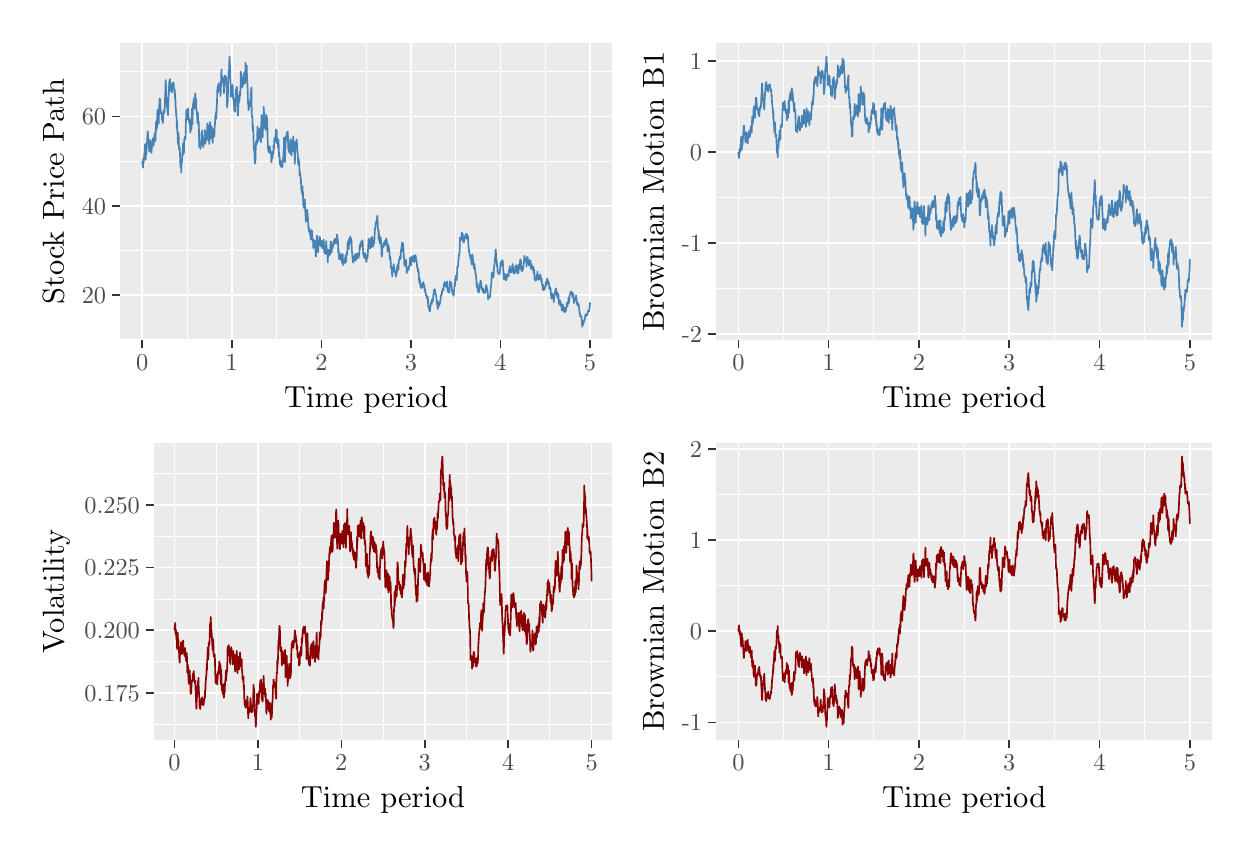
\begin{tikzpicture}[x=1pt,y=1pt]
\definecolor{fillColor}{RGB}{255,255,255}
\path[use as bounding box,fill=fillColor,fill opacity=0.00] (0,0) rectangle (433.62,289.08);
\begin{scope}
\path[clip] (  0.00,144.54) rectangle (216.81,289.08);
\definecolor{drawColor}{RGB}{255,255,255}
\definecolor{fillColor}{RGB}{255,255,255}

\path[draw=drawColor,line width= 0.6pt,line join=round,line cap=round,fill=fillColor] (  0.00,144.54) rectangle (216.81,289.08);
\end{scope}
\begin{scope}
\path[clip] ( 33.30,176.07) rectangle (211.31,283.58);
\definecolor{fillColor}{gray}{0.92}

\path[fill=fillColor] ( 33.30,176.07) rectangle (211.31,283.58);
\definecolor{drawColor}{RGB}{255,255,255}

\path[draw=drawColor,line width= 0.3pt,line join=round] ( 33.30,176.28) --
	(211.31,176.28);

\path[draw=drawColor,line width= 0.3pt,line join=round] ( 33.30,208.57) --
	(211.31,208.57);

\path[draw=drawColor,line width= 0.3pt,line join=round] ( 33.30,240.86) --
	(211.31,240.86);

\path[draw=drawColor,line width= 0.3pt,line join=round] ( 33.30,273.15) --
	(211.31,273.15);

\path[draw=drawColor,line width= 0.3pt,line join=round] ( 57.57,176.07) --
	( 57.57,283.58);

\path[draw=drawColor,line width= 0.3pt,line join=round] ( 89.94,176.07) --
	( 89.94,283.58);

\path[draw=drawColor,line width= 0.3pt,line join=round] (122.30,176.07) --
	(122.30,283.58);

\path[draw=drawColor,line width= 0.3pt,line join=round] (154.67,176.07) --
	(154.67,283.58);

\path[draw=drawColor,line width= 0.3pt,line join=round] (187.04,176.07) --
	(187.04,283.58);

\path[draw=drawColor,line width= 0.6pt,line join=round] ( 33.30,192.43) --
	(211.31,192.43);

\path[draw=drawColor,line width= 0.6pt,line join=round] ( 33.30,224.71) --
	(211.31,224.71);

\path[draw=drawColor,line width= 0.6pt,line join=round] ( 33.30,257.00) --
	(211.31,257.00);

\path[draw=drawColor,line width= 0.6pt,line join=round] ( 41.39,176.07) --
	( 41.39,283.58);

\path[draw=drawColor,line width= 0.6pt,line join=round] ( 73.75,176.07) --
	( 73.75,283.58);

\path[draw=drawColor,line width= 0.6pt,line join=round] (106.12,176.07) --
	(106.12,283.58);

\path[draw=drawColor,line width= 0.6pt,line join=round] (138.49,176.07) --
	(138.49,283.58);

\path[draw=drawColor,line width= 0.6pt,line join=round] (170.85,176.07) --
	(170.85,283.58);

\path[draw=drawColor,line width= 0.6pt,line join=round] (203.22,176.07) --
	(203.22,283.58);
\definecolor{drawColor}{RGB}{70,130,180}

\path[draw=drawColor,line width= 0.6pt,line join=round] ( 41.39,240.86) --
	( 41.48,239.67) --
	( 41.56,240.02) --
	( 41.65,238.45) --
	( 41.74,241.40) --
	( 41.83,242.02) --
	( 41.92,240.46) --
	( 42.01,241.37) --
	( 42.10,242.78) --
	( 42.19,243.88) --
	( 42.27,243.29) --
	( 42.36,246.21) --
	( 42.45,246.98) --
	( 42.54,245.74) --
	( 42.63,241.37) --
	( 42.72,243.51) --
	( 42.81,243.42) --
	( 42.89,243.39) --
	( 42.98,245.21) --
	( 43.07,246.82) --
	( 43.16,248.01) --
	( 43.25,249.85) --
	( 43.34,251.45) --
	( 43.43,251.60) --
	( 43.52,247.48) --
	( 43.60,248.73) --
	( 43.69,248.61) --
	( 43.78,248.30) --
	( 43.87,245.33) --
	( 43.96,244.39) --
	( 44.05,245.21) --
	( 44.14,247.87) --
	( 44.22,247.67) --
	( 44.31,248.45) --
	( 44.40,248.34) --
	( 44.49,245.56) --
	( 44.58,244.74) --
	( 44.67,243.97) --
	( 44.76,243.86) --
	( 44.85,245.99) --
	( 44.93,247.50) --
	( 45.02,247.17) --
	( 45.11,246.66) --
	( 45.20,248.05) --
	( 45.29,249.17) --
	( 45.38,247.77) --
	( 45.47,246.35) --
	( 45.56,247.07) --
	( 45.64,248.61) --
	( 45.73,248.38) --
	( 45.82,250.16) --
	( 45.91,250.97) --
	( 46.00,249.71) --
	( 46.09,250.41) --
	( 46.18,248.09) --
	( 46.26,250.97) --
	( 46.35,255.05) --
	( 46.44,254.27) --
	( 46.53,252.06) --
	( 46.62,253.25) --
	( 46.71,252.96) --
	( 46.80,257.99) --
	( 46.89,257.90) --
	( 46.97,259.40) --
	( 47.06,259.46) --
	( 47.15,257.83) --
	( 47.24,258.24) --
	( 47.33,254.31) --
	( 47.42,257.41) --
	( 47.51,257.74) --
	( 47.59,262.45) --
	( 47.68,263.52) --
	( 47.77,261.91) --
	( 47.86,263.28) --
	( 47.95,261.17) --
	( 48.04,258.38) --
	( 48.13,259.02) --
	( 48.22,258.05) --
	( 48.30,258.05) --
	( 48.39,258.21) --
	( 48.48,256.93) --
	( 48.57,255.70) --
	( 48.66,255.41) --
	( 48.75,257.92) --
	( 48.84,254.61) --
	( 48.92,255.87) --
	( 49.01,256.58) --
	( 49.10,258.87) --
	( 49.19,258.21) --
	( 49.28,259.01) --
	( 49.37,259.60) --
	( 49.46,258.40) --
	( 49.55,261.04) --
	( 49.63,263.62) --
	( 49.72,265.21) --
	( 49.81,268.84) --
	( 49.90,270.15) --
	( 49.99,267.13) --
	( 50.08,265.80) --
	( 50.17,262.98) --
	( 50.25,261.92) --
	( 50.34,260.53) --
	( 50.43,260.62) --
	( 50.52,258.60) --
	( 50.61,258.95) --
	( 50.70,257.51) --
	( 50.79,261.34) --
	( 50.88,262.94) --
	( 50.96,265.00) --
	( 51.05,265.87) --
	( 51.14,269.74) --
	( 51.23,268.24) --
	( 51.32,267.16) --
	( 51.41,270.49) --
	( 51.50,268.95) --
	( 51.58,268.46) --
	( 51.67,267.54) --
	( 51.76,266.79) --
	( 51.85,266.15) --
	( 51.94,267.29) --
	( 52.03,266.88) --
	( 52.12,265.70) --
	( 52.21,268.79) --
	( 52.29,268.29) --
	( 52.38,267.87) --
	( 52.47,267.63) --
	( 52.56,269.30) --
	( 52.65,269.12) --
	( 52.74,269.03) --
	( 52.83,267.43) --
	( 52.92,266.67) --
	( 53.00,266.81) --
	( 53.09,265.45) --
	( 53.18,266.67) --
	( 53.27,263.15) --
	( 53.36,263.84) --
	( 53.45,260.35) --
	( 53.54,259.68) --
	( 53.62,258.52) --
	( 53.71,257.09) --
	( 53.80,256.96) --
	( 53.89,252.82) --
	( 53.98,255.29) --
	( 54.07,251.73) --
	( 54.16,250.77) --
	( 54.25,248.47) --
	( 54.33,246.95) --
	( 54.42,251.12) --
	( 54.51,251.15) --
	( 54.60,248.49) --
	( 54.69,245.17) --
	( 54.78,246.06) --
	( 54.87,246.02) --
	( 54.95,245.39) --
	( 55.04,243.56) --
	( 55.13,240.68) --
	( 55.22,238.65) --
	( 55.31,240.50) --
	( 55.40,239.33) --
	( 55.49,236.75) --
	( 55.58,240.15) --
	( 55.66,240.95) --
	( 55.75,240.49) --
	( 55.84,242.49) --
	( 55.93,244.19) --
	( 56.02,242.98) --
	( 56.11,247.23) --
	( 56.20,246.72) --
	( 56.28,243.89) --
	( 56.37,243.61) --
	( 56.46,244.01) --
	( 56.55,248.49) --
	( 56.64,248.71) --
	( 56.73,249.63) --
	( 56.82,249.47) --
	( 56.91,248.79) --
	( 56.99,248.72) --
	( 57.08,250.32) --
	( 57.17,254.57) --
	( 57.26,256.75) --
	( 57.35,259.35) --
	( 57.44,256.65) --
	( 57.53,258.77) --
	( 57.61,259.25) --
	( 57.70,256.03) --
	( 57.79,257.14) --
	( 57.88,256.80) --
	( 57.97,259.96) --
	( 58.06,258.27) --
	( 58.15,257.33) --
	( 58.24,255.32) --
	( 58.32,254.95) --
	( 58.41,255.80) --
	( 58.50,254.24) --
	( 58.59,255.99) --
	( 58.68,253.40) --
	( 58.77,251.20) --
	( 58.86,254.18) --
	( 58.94,252.03) --
	( 59.03,252.88) --
	( 59.12,252.09) --
	( 59.21,252.94) --
	( 59.30,256.47) --
	( 59.39,259.89) --
	( 59.48,259.16) --
	( 59.57,254.14) --
	( 59.65,259.42) --
	( 59.74,260.88) --
	( 59.83,262.09) --
	( 59.92,262.06) --
	( 60.01,263.20) --
	( 60.10,262.83) --
	( 60.19,263.77) --
	( 60.28,262.87) --
	( 60.36,259.78) --
	( 60.45,261.96) --
	( 60.54,265.36) --
	( 60.63,264.65) --
	( 60.72,261.79) --
	( 60.81,263.23) --
	( 60.90,263.13) --
	( 60.98,259.22) --
	( 61.07,259.22) --
	( 61.16,257.84) --
	( 61.25,257.10) --
	( 61.34,254.60) --
	( 61.43,258.42) --
	( 61.52,257.70) --
	( 61.61,254.21) --
	( 61.69,254.63) --
	( 61.78,255.19) --
	( 61.87,253.09) --
	( 61.96,247.03) --
	( 62.05,245.76) --
	( 62.14,246.88) --
	( 62.23,246.76) --
	( 62.31,246.57) --
	( 62.40,247.68) --
	( 62.49,245.30) --
	( 62.58,247.46) --
	( 62.67,247.45) --
	( 62.76,248.86) --
	( 62.85,250.95) --
	( 62.94,251.42) --
	( 63.02,249.60) --
	( 63.11,251.97) --
	( 63.20,247.82) --
	( 63.29,246.72) --
	( 63.38,246.21) --
	( 63.47,245.89) --
	( 63.56,247.90) --
	( 63.64,248.17) --
	( 63.73,248.99) --
	( 63.82,248.85) --
	( 63.91,248.35) --
	( 64.00,249.75) --
	( 64.09,252.09) --
	( 64.18,247.10) --
	( 64.27,248.24) --
	( 64.35,248.99) --
	( 64.44,248.13) --
	( 64.53,250.04) --
	( 64.62,249.25) --
	( 64.71,248.67) --
	( 64.80,250.40) --
	( 64.89,253.93) --
	( 64.97,254.49) --
	( 65.06,253.60) --
	( 65.15,251.10) --
	( 65.24,250.42) --
	( 65.33,248.49) --
	( 65.42,247.97) --
	( 65.51,248.76) --
	( 65.60,247.04) --
	( 65.68,252.32) --
	( 65.77,252.64) --
	( 65.86,255.00) --
	( 65.95,250.14) --
	( 66.04,251.65) --
	( 66.13,248.93) --
	( 66.22,250.79) --
	( 66.30,251.61) --
	( 66.39,250.77) --
	( 66.48,253.49) --
	( 66.57,252.02) --
	( 66.66,250.81) --
	( 66.75,248.75) --
	( 66.84,247.41) --
	( 66.93,249.29) --
	( 67.01,250.17) --
	( 67.10,252.23) --
	( 67.19,251.42) --
	( 67.28,252.19) --
	( 67.37,252.70) --
	( 67.46,249.73) --
	( 67.55,253.35) --
	( 67.64,253.63) --
	( 67.72,255.24) --
	( 67.81,257.27) --
	( 67.90,257.16) --
	( 67.99,256.50) --
	( 68.08,258.42) --
	( 68.17,256.14) --
	( 68.26,260.36) --
	( 68.34,259.51) --
	( 68.43,263.14) --
	( 68.52,266.55) --
	( 68.61,266.74) --
	( 68.70,268.05) --
	( 68.79,265.66) --
	( 68.88,266.40) --
	( 68.97,268.81) --
	( 69.05,269.04) --
	( 69.14,267.97) --
	( 69.23,266.45) --
	( 69.32,266.36) --
	( 69.41,268.83) --
	( 69.50,267.69) --
	( 69.59,267.41) --
	( 69.67,264.41) --
	( 69.76,265.53) --
	( 69.85,268.53) --
	( 69.94,272.03) --
	( 70.03,273.98) --
	( 70.12,269.46) --
	( 70.21,270.59) --
	( 70.30,271.67) --
	( 70.38,270.83) --
	( 70.47,271.23) --
	( 70.56,269.17) --
	( 70.65,270.77) --
	( 70.74,269.99) --
	( 70.83,266.29) --
	( 70.92,265.44) --
	( 71.00,268.57) --
	( 71.09,267.79) --
	( 71.18,269.49) --
	( 71.27,271.72) --
	( 71.36,271.73) --
	( 71.45,270.89) --
	( 71.54,269.63) --
	( 71.63,271.38) --
	( 71.71,268.84) --
	( 71.80,269.42) --
	( 71.89,268.74) --
	( 71.98,263.42) --
	( 72.07,260.24) --
	( 72.16,262.26) --
	( 72.25,261.83) --
	( 72.33,263.63) --
	( 72.42,267.91) --
	( 72.51,271.34) --
	( 72.60,272.96) --
	( 72.69,273.87) --
	( 72.78,273.41) --
	( 72.87,277.22) --
	( 72.96,278.69) --
	( 73.04,275.77) --
	( 73.13,275.39) --
	( 73.22,270.69) --
	( 73.31,270.23) --
	( 73.40,264.09) --
	( 73.49,267.07) --
	( 73.58,265.60) --
	( 73.66,264.61) --
	( 73.75,264.23) --
	( 73.84,265.62) --
	( 73.93,267.18) --
	( 74.02,268.50) --
	( 74.11,267.16) --
	( 74.20,263.99) --
	( 74.29,263.11) --
	( 74.37,263.73) --
	( 74.46,261.87) --
	( 74.55,261.71) --
	( 74.64,259.10) --
	( 74.73,259.08) --
	( 74.82,259.36) --
	( 74.91,259.04) --
	( 75.00,258.68) --
	( 75.08,262.55) --
	( 75.17,264.26) --
	( 75.26,266.80) --
	( 75.35,264.66) --
	( 75.44,265.03) --
	( 75.53,267.68) --
	( 75.62,267.54) --
	( 75.70,262.58) --
	( 75.79,263.36) --
	( 75.88,259.04) --
	( 75.97,257.26) --
	( 76.06,260.13) --
	( 76.15,261.50) --
	( 76.24,263.94) --
	( 76.33,264.63) --
	( 76.41,264.38) --
	( 76.50,262.27) --
	( 76.59,265.85) --
	( 76.68,265.96) --
	( 76.77,264.31) --
	( 76.86,266.28) --
	( 76.95,268.77) --
	( 77.03,273.22) --
	( 77.12,271.76) --
	( 77.21,270.83) --
	( 77.30,269.83) --
	( 77.39,268.95) --
	( 77.48,268.08) --
	( 77.57,267.39) --
	( 77.66,270.75) --
	( 77.74,269.09) --
	( 77.83,268.17) --
	( 77.92,269.70) --
	( 78.01,272.36) --
	( 78.10,270.51) --
	( 78.19,269.30) --
	( 78.28,270.53) --
	( 78.36,272.95) --
	( 78.45,272.35) --
	( 78.54,268.91) --
	( 78.63,272.93) --
	( 78.72,276.40) --
	( 78.81,274.64) --
	( 78.90,274.49) --
	( 78.99,270.19) --
	( 79.07,271.55) --
	( 79.16,275.41) --
	( 79.25,271.39) --
	( 79.34,269.53) --
	( 79.43,268.01) --
	( 79.52,266.42) --
	( 79.61,261.70) --
	( 79.69,262.83) --
	( 79.78,259.37) --
	( 79.87,259.31) --
	( 79.96,260.62) --
	( 80.05,260.18) --
	( 80.14,262.16) --
	( 80.23,262.10) --
	( 80.32,260.64) --
	( 80.40,262.08) --
	( 80.49,261.10) --
	( 80.58,265.06) --
	( 80.67,265.02) --
	( 80.76,266.98) --
	( 80.85,267.46) --
	( 80.94,260.44) --
	( 81.02,257.40) --
	( 81.11,256.48) --
	( 81.20,256.99) --
	( 81.29,251.91) --
	( 81.38,253.92) --
	( 81.47,252.64) --
	( 81.56,251.06) --
	( 81.65,247.84) --
	( 81.73,244.91) --
	( 81.82,245.02) --
	( 81.91,246.02) --
	( 82.00,241.86) --
	( 82.09,239.95) --
	( 82.18,240.95) --
	( 82.27,240.09) --
	( 82.36,244.16) --
	( 82.44,246.59) --
	( 82.53,247.78) --
	( 82.62,247.79) --
	( 82.71,248.35) --
	( 82.80,246.92) --
	( 82.89,248.17) --
	( 82.98,251.16) --
	( 83.06,253.40) --
	( 83.15,251.69) --
	( 83.24,248.33) --
	( 83.33,248.11) --
	( 83.42,249.00) --
	( 83.51,251.74) --
	( 83.60,249.00) --
	( 83.69,249.74) --
	( 83.77,250.22) --
	( 83.86,252.67) --
	( 83.95,252.61) --
	( 84.04,251.86) --
	( 84.13,249.48) --
	( 84.22,248.42) --
	( 84.31,247.69) --
	( 84.39,252.41) --
	( 84.48,257.52) --
	( 84.57,257.16) --
	( 84.66,254.90) --
	( 84.75,250.70) --
	( 84.84,251.76) --
	( 84.93,249.50) --
	( 85.02,254.15) --
	( 85.10,252.28) --
	( 85.19,252.51) --
	( 85.28,260.47) --
	( 85.37,258.01) --
	( 85.46,258.68) --
	( 85.55,256.26) --
	( 85.64,257.01) --
	( 85.72,255.12) --
	( 85.81,255.29) --
	( 85.90,254.65) --
	( 85.99,252.14) --
	( 86.08,252.17) --
	( 86.17,254.23) --
	( 86.26,257.60) --
	( 86.35,254.62) --
	( 86.43,254.09) --
	( 86.52,256.54) --
	( 86.61,254.14) --
	( 86.70,248.80) --
	( 86.79,246.91) --
	( 86.88,244.98) --
	( 86.97,245.07) --
	( 87.05,244.28) --
	( 87.14,244.73) --
	( 87.23,243.91) --
	( 87.32,244.63) --
	( 87.41,243.92) --
	( 87.50,246.23) --
	( 87.59,244.77) --
	( 87.68,245.34) --
	( 87.76,243.60) --
	( 87.85,244.00) --
	( 87.94,243.91) --
	( 88.03,240.64) --
	( 88.12,240.37) --
	( 88.21,242.59) --
	( 88.30,243.89) --
	( 88.38,244.17) --
	( 88.47,241.85) --
	( 88.56,244.08) --
	( 88.65,244.23) --
	( 88.74,243.35) --
	( 88.83,246.52) --
	( 88.92,244.99) --
	( 89.01,245.59) --
	( 89.09,248.11) --
	( 89.18,249.32) --
	( 89.27,248.70) --
	( 89.36,247.85) --
	( 89.45,248.56) --
	( 89.54,249.60) --
	( 89.63,249.64) --
	( 89.72,252.32) --
	( 89.80,252.19) --
	( 89.89,250.73) --
	( 89.98,251.83) --
	( 90.07,247.27) --
	( 90.16,248.05) --
	( 90.25,249.05) --
	( 90.34,248.60) --
	( 90.42,246.34) --
	( 90.51,245.56) --
	( 90.60,248.61) --
	( 90.69,247.11) --
	( 90.78,242.46) --
	( 90.87,244.01) --
	( 90.96,243.04) --
	( 91.05,242.06) --
	( 91.13,239.74) --
	( 91.22,239.70) --
	( 91.31,241.01) --
	( 91.40,239.90) --
	( 91.49,238.77) --
	( 91.58,240.79) --
	( 91.67,240.33) --
	( 91.75,240.03) --
	( 91.84,238.86) --
	( 91.93,240.52) --
	( 92.02,238.65) --
	( 92.11,240.22) --
	( 92.20,241.73) --
	( 92.29,240.84) --
	( 92.38,242.44) --
	( 92.46,244.33) --
	( 92.55,245.44) --
	( 92.64,249.42) --
	( 92.73,245.44) --
	( 92.82,243.15) --
	( 92.91,240.51) --
	( 93.00,240.82) --
	( 93.08,243.80) --
	( 93.17,247.04) --
	( 93.26,248.02) --
	( 93.35,249.78) --
	( 93.44,249.48) --
	( 93.53,250.43) --
	( 93.62,251.20) --
	( 93.71,249.64) --
	( 93.79,249.04) --
	( 93.88,248.77) --
	( 93.97,251.58) --
	( 94.06,249.44) --
	( 94.15,245.15) --
	( 94.24,246.65) --
	( 94.33,245.04) --
	( 94.41,244.19) --
	( 94.50,245.94) --
	( 94.59,244.44) --
	( 94.68,243.77) --
	( 94.77,246.68) --
	( 94.86,247.72) --
	( 94.95,248.81) --
	( 95.04,248.53) --
	( 95.12,246.24) --
	( 95.21,243.29) --
	( 95.30,242.86) --
	( 95.39,246.70) --
	( 95.48,247.13) --
	( 95.57,247.46) --
	( 95.66,248.12) --
	( 95.74,247.35) --
	( 95.83,244.57) --
	( 95.92,249.77) --
	( 96.01,248.91) --
	( 96.10,248.31) --
	( 96.19,244.71) --
	( 96.28,244.23) --
	( 96.37,243.75) --
	( 96.45,243.25) --
	( 96.54,239.82) --
	( 96.63,243.14) --
	( 96.72,246.53) --
	( 96.81,247.89) --
	( 96.90,245.69) --
	( 96.99,247.09) --
	( 97.08,246.60) --
	( 97.16,245.97) --
	( 97.25,248.65) --
	( 97.34,246.18) --
	( 97.43,245.17) --
	( 97.52,243.74) --
	( 97.61,243.78) --
	( 97.70,240.75) --
	( 97.78,239.43) --
	( 97.87,240.76) --
	( 97.96,241.63) --
	( 98.05,239.79) --
	( 98.14,240.83) --
	( 98.23,236.26) --
	( 98.32,235.65) --
	( 98.41,236.92) --
	( 98.49,235.73) --
	( 98.58,235.67) --
	( 98.67,232.82) --
	( 98.76,234.29) --
	( 98.85,231.04) --
	( 98.94,230.48) --
	( 99.03,230.05) --
	( 99.11,230.16) --
	( 99.20,228.77) --
	( 99.29,231.80) --
	( 99.38,229.35) --
	( 99.47,229.78) --
	( 99.56,224.85) --
	( 99.65,224.85) --
	( 99.74,225.66) --
	( 99.82,223.93) --
	( 99.91,225.03) --
	(100.00,225.55) --
	(100.09,227.11) --
	(100.18,225.74) --
	(100.27,224.19) --
	(100.36,221.41) --
	(100.44,220.92) --
	(100.53,218.90) --
	(100.62,219.91) --
	(100.71,220.02) --
	(100.80,223.28) --
	(100.89,221.48) --
	(100.98,223.28) --
	(101.07,222.46) --
	(101.15,220.22) --
	(101.24,221.08) --
	(101.33,218.92) --
	(101.42,217.37) --
	(101.51,216.32) --
	(101.60,216.62) --
	(101.69,215.20) --
	(101.77,216.70) --
	(101.86,214.99) --
	(101.95,215.29) --
	(102.04,215.49) --
	(102.13,214.00) --
	(102.22,213.42) --
	(102.31,212.53) --
	(102.40,213.81) --
	(102.48,215.93) --
	(102.57,214.47) --
	(102.66,215.75) --
	(102.75,215.65) --
	(102.84,212.89) --
	(102.93,211.88) --
	(103.02,212.49) --
	(103.10,212.68) --
	(103.19,209.42) --
	(103.28,210.15) --
	(103.37,211.00) --
	(103.46,210.60) --
	(103.55,209.68) --
	(103.64,212.20) --
	(103.73,212.08) --
	(103.81,212.06) --
	(103.90,210.57) --
	(103.99,208.84) --
	(104.08,206.92) --
	(104.17,206.41) --
	(104.26,208.05) --
	(104.35,210.22) --
	(104.43,212.24) --
	(104.52,213.96) --
	(104.61,213.63) --
	(104.70,211.98) --
	(104.79,211.55) --
	(104.88,208.39) --
	(104.97,208.00) --
	(105.06,210.05) --
	(105.14,210.22) --
	(105.23,211.62) --
	(105.32,212.26) --
	(105.41,211.23) --
	(105.50,213.50) --
	(105.59,213.39) --
	(105.68,212.08) --
	(105.77,212.18) --
	(105.85,210.17) --
	(105.94,211.28) --
	(106.03,211.93) --
	(106.12,211.46) --
	(106.21,210.83) --
	(106.30,212.04) --
	(106.39,210.64) --
	(106.47,209.37) --
	(106.56,209.91) --
	(106.65,209.33) --
	(106.74,210.50) --
	(106.83,210.24) --
	(106.92,211.77) --
	(107.01,212.42) --
	(107.10,209.45) --
	(107.18,207.77) --
	(107.27,209.34) --
	(107.36,210.21) --
	(107.45,208.98) --
	(107.54,207.29) --
	(107.63,208.55) --
	(107.72,207.54) --
	(107.80,209.74) --
	(107.89,211.98) --
	(107.98,210.08) --
	(108.07,209.01) --
	(108.16,207.44) --
	(108.25,208.26) --
	(108.34,206.66) --
	(108.43,204.22) --
	(108.51,206.54) --
	(108.60,207.75) --
	(108.69,208.75) --
	(108.78,207.92) --
	(108.87,207.91) --
	(108.96,208.67) --
	(109.05,207.08) --
	(109.13,206.93) --
	(109.22,207.14) --
	(109.31,209.19) --
	(109.40,209.99) --
	(109.49,211.61) --
	(109.58,211.79) --
	(109.67,210.34) --
	(109.76,209.91) --
	(109.84,207.81) --
	(109.93,208.94) --
	(110.02,210.70) --
	(110.11,210.62) --
	(110.20,209.37) --
	(110.29,210.73) --
	(110.38,210.91) --
	(110.46,210.42) --
	(110.55,211.84) --
	(110.64,210.86) --
	(110.73,212.33) --
	(110.82,211.23) --
	(110.91,211.73) --
	(111.00,212.88) --
	(111.09,211.12) --
	(111.17,211.63) --
	(111.26,211.49) --
	(111.35,212.36) --
	(111.44,211.33) --
	(111.53,211.22) --
	(111.62,213.00) --
	(111.71,213.22) --
	(111.79,214.31) --
	(111.88,214.01) --
	(111.97,212.63) --
	(112.06,212.62) --
	(112.15,211.01) --
	(112.24,207.69) --
	(112.33,209.11) --
	(112.42,207.76) --
	(112.50,205.54) --
	(112.59,206.70) --
	(112.68,206.69) --
	(112.77,205.98) --
	(112.86,205.77) --
	(112.95,205.27) --
	(113.04,206.43) --
	(113.13,207.29) --
	(113.21,205.21) --
	(113.30,205.62) --
	(113.39,206.47) --
	(113.48,207.26) --
	(113.57,204.35) --
	(113.66,204.08) --
	(113.75,206.33) --
	(113.83,207.27) --
	(113.92,205.22) --
	(114.01,203.29) --
	(114.10,203.84) --
	(114.19,203.65) --
	(114.28,204.73) --
	(114.37,205.07) --
	(114.46,205.16) --
	(114.54,205.37) --
	(114.63,205.56) --
	(114.72,204.09) --
	(114.81,206.75) --
	(114.90,205.07) --
	(114.99,205.05) --
	(115.08,204.43) --
	(115.16,206.48) --
	(115.25,207.67) --
	(115.34,206.99) --
	(115.43,207.24) --
	(115.52,208.63) --
	(115.61,211.36) --
	(115.70,211.75) --
	(115.79,210.41) --
	(115.87,209.18) --
	(115.96,211.65) --
	(116.05,209.00) --
	(116.14,212.75) --
	(116.23,212.41) --
	(116.32,211.82) --
	(116.41,212.02) --
	(116.49,213.22) --
	(116.58,213.62) --
	(116.67,211.05) --
	(116.76,211.49) --
	(116.85,212.07) --
	(116.94,212.92) --
	(117.03,211.57) --
	(117.12,208.55) --
	(117.20,208.15) --
	(117.29,207.01) --
	(117.38,206.10) --
	(117.47,204.99) --
	(117.56,204.54) --
	(117.65,204.18) --
	(117.74,205.08) --
	(117.82,206.21) --
	(117.91,205.28) --
	(118.00,204.93) --
	(118.09,205.34) --
	(118.18,206.95) --
	(118.27,206.88) --
	(118.36,204.88) --
	(118.45,205.14) --
	(118.53,205.01) --
	(118.62,207.03) --
	(118.71,207.44) --
	(118.80,206.70) --
	(118.89,206.18) --
	(118.98,205.59) --
	(119.07,205.80) --
	(119.15,206.01) --
	(119.24,207.07) --
	(119.33,207.45) --
	(119.42,207.01) --
	(119.51,205.90) --
	(119.60,206.64) --
	(119.69,206.57) --
	(119.78,206.78) --
	(119.86,208.08) --
	(119.95,210.18) --
	(120.04,209.00) --
	(120.13,211.00) --
	(120.22,209.91) --
	(120.31,210.24) --
	(120.40,210.52) --
	(120.49,210.17) --
	(120.57,211.90) --
	(120.66,211.06) --
	(120.75,211.89) --
	(120.84,211.88) --
	(120.93,210.69) --
	(121.02,212.21) --
	(121.11,209.54) --
	(121.19,208.89) --
	(121.28,207.02) --
	(121.37,207.25) --
	(121.46,207.56) --
	(121.55,206.23) --
	(121.64,206.99) --
	(121.73,205.77) --
	(121.82,206.53) --
	(121.90,206.81) --
	(121.99,207.65) --
	(122.08,206.53) --
	(122.17,206.65) --
	(122.26,206.10) --
	(122.35,204.40) --
	(122.44,204.58) --
	(122.52,206.58) --
	(122.61,205.82) --
	(122.70,205.59) --
	(122.79,206.38) --
	(122.88,206.42) --
	(122.97,208.68) --
	(123.06,209.57) --
	(123.15,212.41) --
	(123.23,212.86) --
	(123.32,211.40) --
	(123.41,211.93) --
	(123.50,210.76) --
	(123.59,209.50) --
	(123.68,209.27) --
	(123.77,210.41) --
	(123.85,210.84) --
	(123.94,211.85) --
	(124.03,213.01) --
	(124.12,212.79) --
	(124.21,209.71) --
	(124.30,210.68) --
	(124.39,213.37) --
	(124.48,213.45) --
	(124.56,211.70) --
	(124.65,211.23) --
	(124.74,210.06) --
	(124.83,210.01) --
	(124.92,210.84) --
	(125.01,211.92) --
	(125.10,212.22) --
	(125.18,211.03) --
	(125.27,212.05) --
	(125.36,213.75) --
	(125.45,216.68) --
	(125.54,216.01) --
	(125.63,216.65) --
	(125.72,218.26) --
	(125.81,218.10) --
	(125.89,218.82) --
	(125.98,219.12) --
	(126.07,218.93) --
	(126.16,219.17) --
	(126.25,220.51) --
	(126.34,221.09) --
	(126.43,220.43) --
	(126.51,217.25) --
	(126.60,216.17) --
	(126.69,216.14) --
	(126.78,212.77) --
	(126.87,215.59) --
	(126.96,213.62) --
	(127.05,212.11) --
	(127.14,213.96) --
	(127.22,211.11) --
	(127.31,212.03) --
	(127.40,211.60) --
	(127.49,212.17) --
	(127.58,213.28) --
	(127.67,212.05) --
	(127.76,211.16) --
	(127.85,207.43) --
	(127.93,206.30) --
	(128.02,206.74) --
	(128.11,207.32) --
	(128.20,209.70) --
	(128.29,209.78) --
	(128.38,210.34) --
	(128.47,210.43) --
	(128.55,209.83) --
	(128.64,210.75) --
	(128.73,211.32) --
	(128.82,211.48) --
	(128.91,210.46) --
	(129.00,210.41) --
	(129.09,211.37) --
	(129.18,212.22) --
	(129.26,211.61) --
	(129.35,210.77) --
	(129.44,211.40) --
	(129.53,212.71) --
	(129.62,212.87) --
	(129.71,212.47) --
	(129.80,211.35) --
	(129.88,210.83) --
	(129.97,209.00) --
	(130.06,208.16) --
	(130.15,209.50) --
	(130.24,210.85) --
	(130.33,209.77) --
	(130.42,210.03) --
	(130.51,210.11) --
	(130.59,208.08) --
	(130.68,209.04) --
	(130.77,206.75) --
	(130.86,205.30) --
	(130.95,206.43) --
	(131.04,205.81) --
	(131.13,205.56) --
	(131.21,203.73) --
	(131.30,202.13) --
	(131.39,202.51) --
	(131.48,202.32) --
	(131.57,201.69) --
	(131.66,200.28) --
	(131.75,199.15) --
	(131.84,201.20) --
	(131.92,200.86) --
	(132.01,201.66) --
	(132.10,202.49) --
	(132.19,203.30) --
	(132.28,203.62) --
	(132.37,202.26) --
	(132.46,201.18) --
	(132.54,201.97) --
	(132.63,200.58) --
	(132.72,201.12) --
	(132.81,200.57) --
	(132.90,200.16) --
	(132.99,199.35) --
	(133.08,199.12) --
	(133.17,200.00) --
	(133.25,200.46) --
	(133.34,200.22) --
	(133.43,201.11) --
	(133.52,202.83) --
	(133.61,202.83) --
	(133.70,203.33) --
	(133.79,203.63) --
	(133.87,202.57) --
	(133.96,201.58) --
	(134.05,203.59) --
	(134.14,204.55) --
	(134.23,205.37) --
	(134.32,205.54) --
	(134.41,206.08) --
	(134.50,206.25) --
	(134.58,206.30) --
	(134.67,206.56) --
	(134.76,205.40) --
	(134.85,208.10) --
	(134.94,209.04) --
	(135.03,208.74) --
	(135.12,210.18) --
	(135.21,209.41) --
	(135.29,211.46) --
	(135.38,210.98) --
	(135.47,208.13) --
	(135.56,209.73) --
	(135.65,211.09) --
	(135.74,210.14) --
	(135.83,208.43) --
	(135.91,206.27) --
	(136.00,205.97) --
	(136.09,203.90) --
	(136.18,203.01) --
	(136.27,203.18) --
	(136.36,204.10) --
	(136.45,203.21) --
	(136.54,203.07) --
	(136.62,203.35) --
	(136.71,205.20) --
	(136.80,204.13) --
	(136.89,202.38) --
	(136.98,200.42) --
	(137.07,200.99) --
	(137.16,200.93) --
	(137.24,201.72) --
	(137.33,201.58) --
	(137.42,201.99) --
	(137.51,202.22) --
	(137.60,202.25) --
	(137.69,201.59) --
	(137.78,202.91) --
	(137.87,202.47) --
	(137.95,203.18) --
	(138.04,203.35) --
	(138.13,205.27) --
	(138.22,206.06) --
	(138.31,205.68) --
	(138.40,205.67) --
	(138.49,205.53) --
	(138.57,203.20) --
	(138.66,205.02) --
	(138.75,206.19) --
	(138.84,205.33) --
	(138.93,205.75) --
	(139.02,206.02) --
	(139.11,204.75) --
	(139.20,206.39) --
	(139.28,206.11) --
	(139.37,206.32) --
	(139.46,206.77) --
	(139.55,205.64) --
	(139.64,204.43) --
	(139.73,204.37) --
	(139.82,205.00) --
	(139.90,205.09) --
	(139.99,205.87) --
	(140.08,206.24) --
	(140.17,206.86) --
	(140.26,205.26) --
	(140.35,206.01) --
	(140.44,205.12) --
	(140.53,204.61) --
	(140.61,204.49) --
	(140.70,202.69) --
	(140.79,202.58) --
	(140.88,202.12) --
	(140.97,201.36) --
	(141.06,200.79) --
	(141.15,202.06) --
	(141.23,200.75) --
	(141.32,200.53) --
	(141.41,198.01) --
	(141.50,197.36) --
	(141.59,196.88) --
	(141.68,198.34) --
	(141.77,197.40) --
	(141.86,196.57) --
	(141.94,195.26) --
	(142.03,195.43) --
	(142.12,196.48) --
	(142.21,195.36) --
	(142.30,194.97) --
	(142.39,196.21) --
	(142.48,195.57) --
	(142.57,196.20) --
	(142.65,196.56) --
	(142.74,195.34) --
	(142.83,196.45) --
	(142.92,197.19) --
	(143.01,196.73) --
	(143.10,195.88) --
	(143.19,195.52) --
	(143.27,196.26) --
	(143.36,195.74) --
	(143.45,194.02) --
	(143.54,193.90) --
	(143.63,194.57) --
	(143.72,193.54) --
	(143.81,193.33) --
	(143.90,192.28) --
	(143.98,192.37) --
	(144.07,192.26) --
	(144.16,192.23) --
	(144.25,191.71) --
	(144.34,191.12) --
	(144.43,191.83) --
	(144.52,191.92) --
	(144.60,191.77) --
	(144.69,189.09) --
	(144.78,188.11) --
	(144.87,188.68) --
	(144.96,188.37) --
	(145.05,187.45) --
	(145.14,187.13) --
	(145.23,186.86) --
	(145.31,186.49) --
	(145.40,186.85) --
	(145.49,187.95) --
	(145.58,188.69) --
	(145.67,189.64) --
	(145.76,189.38) --
	(145.85,190.04) --
	(145.93,189.26) --
	(146.02,189.15) --
	(146.11,190.84) --
	(146.20,190.83) --
	(146.29,190.58) --
	(146.38,190.11) --
	(146.47,190.73) --
	(146.56,192.42) --
	(146.64,192.77) --
	(146.73,192.55) --
	(146.82,194.29) --
	(146.91,193.61) --
	(147.00,194.59) --
	(147.09,194.21) --
	(147.18,193.32) --
	(147.26,194.36) --
	(147.35,192.78) --
	(147.44,192.52) --
	(147.53,192.54) --
	(147.62,192.16) --
	(147.71,190.80) --
	(147.80,190.28) --
	(147.89,189.05) --
	(147.97,190.52) --
	(148.06,189.04) --
	(148.15,187.43) --
	(148.24,187.94) --
	(148.33,188.61) --
	(148.42,188.46) --
	(148.51,188.31) --
	(148.59,188.85) --
	(148.68,189.91) --
	(148.77,188.67) --
	(148.86,189.66) --
	(148.95,189.81) --
	(149.04,189.54) --
	(149.13,190.52) --
	(149.22,191.27) --
	(149.30,192.31) --
	(149.39,192.06) --
	(149.48,192.71) --
	(149.57,192.95) --
	(149.66,192.52) --
	(149.75,193.99) --
	(149.84,194.13) --
	(149.93,194.08) --
	(150.01,194.54) --
	(150.10,194.88) --
	(150.19,194.26) --
	(150.28,194.21) --
	(150.37,196.48) --
	(150.46,196.41) --
	(150.55,196.14) --
	(150.63,196.80) --
	(150.72,197.17) --
	(150.81,196.67) --
	(150.90,195.68) --
	(150.99,196.44) --
	(151.08,196.55) --
	(151.17,196.99) --
	(151.26,196.72) --
	(151.34,195.21) --
	(151.43,195.27) --
	(151.52,197.39) --
	(151.61,196.03) --
	(151.70,195.14) --
	(151.79,193.96) --
	(151.88,193.65) --
	(151.96,194.83) --
	(152.05,194.69) --
	(152.14,194.47) --
	(152.23,193.35) --
	(152.32,193.40) --
	(152.41,194.28) --
	(152.50,196.24) --
	(152.59,197.43) --
	(152.67,196.62) --
	(152.76,196.16) --
	(152.85,196.71) --
	(152.94,196.70) --
	(153.03,196.96) --
	(153.12,195.75) --
	(153.21,195.37) --
	(153.29,194.55) --
	(153.38,193.74) --
	(153.47,193.12) --
	(153.56,192.77) --
	(153.65,192.77) --
	(153.74,193.30) --
	(153.83,192.87) --
	(153.92,192.15) --
	(154.00,193.48) --
	(154.09,194.32) --
	(154.18,194.92) --
	(154.27,196.42) --
	(154.36,195.53) --
	(154.45,197.35) --
	(154.54,198.48) --
	(154.62,198.77) --
	(154.71,199.37) --
	(154.80,199.43) --
	(154.89,199.32) --
	(154.98,197.81) --
	(155.07,198.50) --
	(155.16,200.52) --
	(155.25,202.58) --
	(155.33,202.75) --
	(155.42,202.64) --
	(155.51,202.82) --
	(155.60,204.00) --
	(155.69,205.54) --
	(155.78,205.98) --
	(155.87,207.19) --
	(155.95,207.16) --
	(156.04,207.71) --
	(156.13,209.03) --
	(156.22,213.16) --
	(156.31,213.09) --
	(156.40,212.29) --
	(156.49,212.82) --
	(156.58,212.33) --
	(156.66,213.09) --
	(156.75,213.50) --
	(156.84,215.09) --
	(156.93,213.90) --
	(157.02,212.44) --
	(157.11,214.31) --
	(157.20,214.58) --
	(157.29,213.45) --
	(157.37,212.15) --
	(157.46,211.50) --
	(157.55,212.19) --
	(157.64,211.56) --
	(157.73,213.14) --
	(157.82,213.44) --
	(157.91,213.67) --
	(157.99,213.65) --
	(158.08,213.29) --
	(158.17,213.09) --
	(158.26,214.48) --
	(158.35,212.84) --
	(158.44,214.14) --
	(158.53,213.72) --
	(158.62,214.61) --
	(158.70,214.54) --
	(158.79,212.88) --
	(158.88,213.30) --
	(158.97,212.53) --
	(159.06,213.87) --
	(159.15,212.87) --
	(159.24,210.72) --
	(159.32,209.73) --
	(159.41,209.07) --
	(159.50,208.14) --
	(159.59,207.87) --
	(159.68,207.21) --
	(159.77,206.76) --
	(159.86,207.11) --
	(159.95,205.83) --
	(160.03,206.65) --
	(160.12,206.65) --
	(160.21,206.61) --
	(160.30,204.39) --
	(160.39,204.07) --
	(160.48,203.49) --
	(160.57,204.37) --
	(160.65,205.83) --
	(160.74,207.15) --
	(160.83,205.93) --
	(160.92,205.07) --
	(161.01,204.98) --
	(161.10,203.85) --
	(161.19,202.18) --
	(161.28,202.98) --
	(161.36,203.05) --
	(161.45,203.68) --
	(161.54,202.43) --
	(161.63,202.09) --
	(161.72,200.91) --
	(161.81,200.09) --
	(161.90,200.31) --
	(161.98,199.52) --
	(162.07,198.56) --
	(162.16,197.33) --
	(162.25,196.01) --
	(162.34,195.24) --
	(162.43,196.74) --
	(162.52,196.14) --
	(162.61,195.15) --
	(162.69,193.92) --
	(162.78,193.79) --
	(162.87,193.46) --
	(162.96,193.67) --
	(163.05,193.43) --
	(163.14,194.16) --
	(163.23,194.77) --
	(163.31,195.69) --
	(163.40,195.91) --
	(163.49,196.90) --
	(163.58,196.83) --
	(163.67,197.67) --
	(163.76,197.53) --
	(163.85,196.90) --
	(163.94,195.79) --
	(164.02,195.16) --
	(164.11,194.51) --
	(164.20,195.01) --
	(164.29,194.96) --
	(164.38,194.41) --
	(164.47,193.64) --
	(164.56,194.92) --
	(164.65,194.71) --
	(164.73,193.63) --
	(164.82,193.27) --
	(164.91,193.35) --
	(165.00,194.04) --
	(165.09,193.97) --
	(165.18,194.07) --
	(165.27,193.18) --
	(165.35,193.85) --
	(165.44,193.93) --
	(165.53,194.56) --
	(165.62,195.89) --
	(165.71,196.05) --
	(165.80,195.79) --
	(165.89,195.12) --
	(165.98,194.61) --
	(166.06,193.83) --
	(166.15,194.14) --
	(166.24,192.89) --
	(166.33,191.45) --
	(166.42,190.91) --
	(166.51,191.77) --
	(166.60,191.87) --
	(166.68,191.47) --
	(166.77,192.00) --
	(166.86,191.72) --
	(166.95,191.63) --
	(167.04,191.68) --
	(167.13,192.56) --
	(167.22,193.62) --
	(167.31,194.69) --
	(167.39,195.53) --
	(167.48,195.82) --
	(167.57,197.48) --
	(167.66,199.35) --
	(167.75,200.61) --
	(167.84,200.39) --
	(167.93,199.39) --
	(168.01,199.57) --
	(168.10,199.04) --
	(168.19,199.30) --
	(168.28,198.78) --
	(168.37,199.64) --
	(168.46,201.73) --
	(168.55,202.68) --
	(168.64,203.43) --
	(168.72,203.47) --
	(168.81,205.70) --
	(168.90,205.61) --
	(168.99,207.07) --
	(169.08,208.78) --
	(169.17,208.95) --
	(169.26,205.32) --
	(169.34,204.98) --
	(169.43,205.46) --
	(169.52,204.08) --
	(169.61,202.75) --
	(169.70,203.66) --
	(169.79,200.80) --
	(169.88,201.03) --
	(169.97,200.77) --
	(170.05,200.13) --
	(170.14,200.19) --
	(170.23,200.24) --
	(170.32,200.48) --
	(170.41,200.60) --
	(170.50,200.08) --
	(170.59,200.33) --
	(170.67,201.66) --
	(170.76,202.32) --
	(170.85,203.81) --
	(170.94,203.53) --
	(171.03,204.13) --
	(171.12,204.65) --
	(171.21,203.87) --
	(171.30,203.04) --
	(171.38,204.93) --
	(171.47,204.06) --
	(171.56,205.04) --
	(171.65,204.76) --
	(171.74,203.62) --
	(171.83,202.05) --
	(171.92,200.86) --
	(172.01,198.96) --
	(172.09,198.13) --
	(172.18,199.03) --
	(172.27,198.49) --
	(172.36,200.10) --
	(172.45,199.93) --
	(172.54,199.04) --
	(172.63,198.77) --
	(172.71,198.22) --
	(172.80,197.81) --
	(172.89,197.87) --
	(172.98,197.94) --
	(173.07,198.64) --
	(173.16,199.14) --
	(173.25,199.87) --
	(173.34,199.99) --
	(173.42,199.22) --
	(173.51,199.65) --
	(173.60,200.04) --
	(173.69,199.65) --
	(173.78,199.28) --
	(173.87,200.31) --
	(173.96,201.60) --
	(174.04,201.71) --
	(174.13,201.33) --
	(174.22,202.94) --
	(174.31,201.69) --
	(174.40,200.79) --
	(174.49,201.62) --
	(174.58,200.71) --
	(174.67,201.57) --
	(174.75,200.65) --
	(174.84,201.17) --
	(174.93,200.99) --
	(175.02,201.85) --
	(175.11,203.17) --
	(175.20,203.06) --
	(175.29,203.68) --
	(175.37,201.85) --
	(175.46,201.59) --
	(175.55,200.40) --
	(175.64,200.60) --
	(175.73,200.58) --
	(175.82,200.36) --
	(175.91,200.18) --
	(176.00,201.09) --
	(176.08,200.94) --
	(176.17,202.73) --
	(176.26,200.83) --
	(176.35,201.18) --
	(176.44,203.23) --
	(176.53,202.09) --
	(176.62,201.30) --
	(176.70,200.91) --
	(176.79,201.00) --
	(176.88,200.77) --
	(176.97,200.32) --
	(177.06,202.17) --
	(177.15,202.29) --
	(177.24,203.37) --
	(177.33,200.37) --
	(177.41,201.45) --
	(177.50,202.73) --
	(177.59,202.24) --
	(177.68,202.02) --
	(177.77,203.67) --
	(177.86,203.71) --
	(177.95,204.76) --
	(178.03,205.37) --
	(178.12,205.20) --
	(178.21,204.90) --
	(178.30,203.43) --
	(178.39,201.27) --
	(178.48,201.25) --
	(178.57,201.51) --
	(178.66,201.02) --
	(178.74,201.63) --
	(178.83,202.09) --
	(178.92,201.76) --
	(179.01,201.80) --
	(179.10,203.08) --
	(179.19,203.39) --
	(179.28,204.20) --
	(179.36,204.70) --
	(179.45,206.48) --
	(179.54,206.59) --
	(179.63,205.53) --
	(179.72,205.05) --
	(179.81,205.30) --
	(179.90,205.02) --
	(179.99,204.84) --
	(180.07,205.53) --
	(180.16,204.72) --
	(180.25,202.74) --
	(180.34,204.75) --
	(180.43,205.20) --
	(180.52,206.29) --
	(180.61,205.96) --
	(180.70,206.06) --
	(180.78,203.79) --
	(180.87,204.15) --
	(180.96,204.63) --
	(181.05,203.70) --
	(181.14,203.16) --
	(181.23,204.51) --
	(181.32,204.99) --
	(181.40,204.73) --
	(181.49,205.11) --
	(181.58,203.71) --
	(181.67,204.90) --
	(181.76,202.93) --
	(181.85,201.93) --
	(181.94,202.59) --
	(182.03,203.73) --
	(182.11,201.98) --
	(182.20,202.57) --
	(182.29,202.91) --
	(182.38,202.87) --
	(182.47,202.25) --
	(182.56,201.40) --
	(182.65,201.55) --
	(182.73,202.73) --
	(182.82,201.25) --
	(182.91,200.23) --
	(183.00,201.78) --
	(183.09,200.60) --
	(183.18,198.09) --
	(183.27,198.11) --
	(183.36,198.42) --
	(183.44,198.43) --
	(183.53,197.63) --
	(183.62,197.94) --
	(183.71,197.78) --
	(183.80,198.61) --
	(183.89,198.89) --
	(183.98,199.53) --
	(184.06,199.84) --
	(184.15,200.22) --
	(184.24,200.94) --
	(184.33,198.74) --
	(184.42,199.22) --
	(184.51,197.96) --
	(184.60,198.29) --
	(184.69,199.50) --
	(184.77,199.08) --
	(184.86,198.33) --
	(184.95,198.25) --
	(185.04,199.69) --
	(185.13,199.79) --
	(185.22,199.93) --
	(185.31,199.41) --
	(185.39,198.92) --
	(185.48,198.79) --
	(185.57,197.33) --
	(185.66,198.43) --
	(185.75,198.12) --
	(185.84,196.30) --
	(185.93,196.29) --
	(186.02,196.08) --
	(186.10,194.51) --
	(186.19,196.24) --
	(186.28,195.26) --
	(186.37,194.11) --
	(186.46,194.48) --
	(186.55,195.35) --
	(186.64,195.18) --
	(186.72,195.38) --
	(186.81,194.43) --
	(186.90,195.23) --
	(186.99,195.50) --
	(187.08,195.59) --
	(187.17,196.23) --
	(187.26,197.11) --
	(187.35,196.45) --
	(187.43,196.88) --
	(187.52,196.00) --
	(187.61,197.94) --
	(187.70,198.35) --
	(187.79,198.32) --
	(187.88,197.87) --
	(187.97,197.67) --
	(188.06,196.68) --
	(188.14,196.74) --
	(188.23,197.25) --
	(188.32,196.79) --
	(188.41,196.08) --
	(188.50,194.66) --
	(188.59,195.14) --
	(188.68,195.42) --
	(188.76,195.24) --
	(188.85,194.77) --
	(188.94,194.99) --
	(189.03,193.82) --
	(189.12,192.61) --
	(189.21,191.45) --
	(189.30,191.16) --
	(189.39,191.78) --
	(189.47,192.34) --
	(189.56,191.89) --
	(189.65,193.01) --
	(189.74,192.08) --
	(189.83,191.69) --
	(189.92,191.11) --
	(190.01,191.24) --
	(190.09,189.88) --
	(190.18,190.77) --
	(190.27,191.69) --
	(190.36,192.46) --
	(190.45,192.39) --
	(190.54,193.31) --
	(190.63,193.71) --
	(190.72,194.50) --
	(190.80,194.65) --
	(190.89,194.89) --
	(190.98,193.11) --
	(191.07,192.67) --
	(191.16,193.48) --
	(191.25,193.57) --
	(191.34,192.57) --
	(191.42,191.80) --
	(191.51,191.37) --
	(191.60,193.01) --
	(191.69,192.87) --
	(191.78,192.35) --
	(191.87,190.69) --
	(191.96,189.24) --
	(192.05,190.13) --
	(192.13,189.49) --
	(192.22,190.69) --
	(192.31,190.44) --
	(192.40,188.68) --
	(192.49,190.26) --
	(192.58,189.45) --
	(192.67,189.08) --
	(192.75,189.15) --
	(192.84,189.06) --
	(192.93,187.95) --
	(193.02,186.88) --
	(193.11,187.84) --
	(193.20,187.34) --
	(193.29,187.92) --
	(193.38,189.12) --
	(193.46,188.55) --
	(193.55,188.04) --
	(193.64,186.64) --
	(193.73,187.92) --
	(193.82,187.39) --
	(193.91,187.13) --
	(194.00,186.19) --
	(194.08,186.69) --
	(194.17,187.78) --
	(194.26,187.94) --
	(194.35,187.66) --
	(194.44,186.49) --
	(194.53,187.50) --
	(194.62,187.98) --
	(194.71,187.95) --
	(194.79,188.80) --
	(194.88,189.73) --
	(194.97,189.39) --
	(195.06,188.49) --
	(195.15,189.18) --
	(195.24,189.69) --
	(195.33,189.32) --
	(195.42,191.62) --
	(195.50,189.65) --
	(195.59,189.64) --
	(195.68,190.48) --
	(195.77,191.59) --
	(195.86,192.35) --
	(195.95,192.46) --
	(196.04,193.08) --
	(196.12,193.53) --
	(196.21,193.51) --
	(196.30,192.80) --
	(196.39,193.77) --
	(196.48,193.48) --
	(196.57,193.24) --
	(196.66,193.45) --
	(196.75,193.46) --
	(196.83,191.86) --
	(196.92,191.53) --
	(197.01,192.00) --
	(197.10,192.96) --
	(197.19,191.95) --
	(197.28,191.44) --
	(197.37,189.57) --
	(197.45,190.30) --
	(197.54,190.30) --
	(197.63,190.89) --
	(197.72,190.46) --
	(197.81,190.62) --
	(197.90,191.36) --
	(197.99,191.18) --
	(198.08,191.82) --
	(198.16,192.33) --
	(198.25,191.08) --
	(198.34,191.32) --
	(198.43,189.42) --
	(198.52,189.22) --
	(198.61,188.82) --
	(198.70,189.44) --
	(198.78,189.66) --
	(198.87,189.22) --
	(198.96,189.11) --
	(199.05,189.24) --
	(199.14,188.51) --
	(199.23,188.02) --
	(199.32,187.15) --
	(199.41,186.11) --
	(199.49,185.76) --
	(199.58,185.75) --
	(199.67,184.72) --
	(199.76,185.02) --
	(199.85,184.59) --
	(199.94,184.79) --
	(200.03,184.88) --
	(200.11,184.64) --
	(200.20,183.41) --
	(200.29,182.44) --
	(200.38,180.96) --
	(200.47,181.71) --
	(200.56,181.51) --
	(200.65,182.60) --
	(200.74,181.74) --
	(200.82,182.59) --
	(200.91,183.22) --
	(201.00,182.76) --
	(201.09,183.19) --
	(201.18,183.53) --
	(201.27,183.45) --
	(201.36,184.36) --
	(201.44,184.18) --
	(201.53,185.44) --
	(201.62,184.67) --
	(201.71,185.49) --
	(201.80,185.15) --
	(201.89,185.38) --
	(201.98,185.33) --
	(202.07,185.25) --
	(202.15,185.19) --
	(202.24,185.78) --
	(202.33,185.80) --
	(202.42,186.68) --
	(202.51,186.76) --
	(202.60,186.88) --
	(202.69,186.84) --
	(202.78,186.56) --
	(202.86,186.69) --
	(202.95,187.36) --
	(203.04,187.91) --
	(203.13,188.60) --
	(203.22,189.82);
\end{scope}
\begin{scope}
\path[clip] (  0.00,  0.00) rectangle (433.62,289.08);
\definecolor{drawColor}{gray}{0.30}

\node[text=drawColor,anchor=base east,inner sep=0pt, outer sep=0pt, scale=  0.88] at ( 28.35,189.39) {20};

\node[text=drawColor,anchor=base east,inner sep=0pt, outer sep=0pt, scale=  0.88] at ( 28.35,221.68) {40};

\node[text=drawColor,anchor=base east,inner sep=0pt, outer sep=0pt, scale=  0.88] at ( 28.35,253.97) {60};
\end{scope}
\begin{scope}
\path[clip] (  0.00,  0.00) rectangle (433.62,289.08);
\definecolor{drawColor}{gray}{0.20}

\path[draw=drawColor,line width= 0.6pt,line join=round] ( 30.55,192.43) --
	( 33.30,192.43);

\path[draw=drawColor,line width= 0.6pt,line join=round] ( 30.55,224.71) --
	( 33.30,224.71);

\path[draw=drawColor,line width= 0.6pt,line join=round] ( 30.55,257.00) --
	( 33.30,257.00);
\end{scope}
\begin{scope}
\path[clip] (  0.00,  0.00) rectangle (433.62,289.08);
\definecolor{drawColor}{gray}{0.20}

\path[draw=drawColor,line width= 0.6pt,line join=round] ( 41.39,173.32) --
	( 41.39,176.07);

\path[draw=drawColor,line width= 0.6pt,line join=round] ( 73.75,173.32) --
	( 73.75,176.07);

\path[draw=drawColor,line width= 0.6pt,line join=round] (106.12,173.32) --
	(106.12,176.07);

\path[draw=drawColor,line width= 0.6pt,line join=round] (138.49,173.32) --
	(138.49,176.07);

\path[draw=drawColor,line width= 0.6pt,line join=round] (170.85,173.32) --
	(170.85,176.07);

\path[draw=drawColor,line width= 0.6pt,line join=round] (203.22,173.32) --
	(203.22,176.07);
\end{scope}
\begin{scope}
\path[clip] (  0.00,  0.00) rectangle (433.62,289.08);
\definecolor{drawColor}{gray}{0.30}

\node[text=drawColor,anchor=base,inner sep=0pt, outer sep=0pt, scale=  0.88] at ( 41.39,165.06) {0};

\node[text=drawColor,anchor=base,inner sep=0pt, outer sep=0pt, scale=  0.88] at ( 73.75,165.06) {1};

\node[text=drawColor,anchor=base,inner sep=0pt, outer sep=0pt, scale=  0.88] at (106.12,165.06) {2};

\node[text=drawColor,anchor=base,inner sep=0pt, outer sep=0pt, scale=  0.88] at (138.49,165.06) {3};

\node[text=drawColor,anchor=base,inner sep=0pt, outer sep=0pt, scale=  0.88] at (170.85,165.06) {4};

\node[text=drawColor,anchor=base,inner sep=0pt, outer sep=0pt, scale=  0.88] at (203.22,165.06) {5};
\end{scope}
\begin{scope}
\path[clip] (  0.00,  0.00) rectangle (433.62,289.08);
\definecolor{drawColor}{RGB}{0,0,0}

\node[text=drawColor,anchor=base,inner sep=0pt, outer sep=0pt, scale=  1.10] at (122.30,151.98) {Time period};
\end{scope}
\begin{scope}
\path[clip] (  0.00,  0.00) rectangle (433.62,289.08);
\definecolor{drawColor}{RGB}{0,0,0}

\node[text=drawColor,rotate= 90.00,anchor=base,inner sep=0pt, outer sep=0pt, scale=  1.10] at ( 13.08,229.83) {Stock Price Path};
\end{scope}
\begin{scope}
\path[clip] (216.81,144.54) rectangle (433.62,289.08);
\definecolor{drawColor}{RGB}{255,255,255}
\definecolor{fillColor}{RGB}{255,255,255}

\path[draw=drawColor,line width= 0.6pt,line join=round,line cap=round,fill=fillColor] (216.81,144.54) rectangle (433.62,289.08);
\end{scope}
\begin{scope}
\path[clip] (248.64,176.07) rectangle (428.12,283.58);
\definecolor{fillColor}{gray}{0.92}

\path[fill=fillColor] (248.64,176.07) rectangle (428.12,283.58);
\definecolor{drawColor}{RGB}{255,255,255}

\path[draw=drawColor,line width= 0.3pt,line join=round] (248.64,194.81) --
	(428.12,194.81);

\path[draw=drawColor,line width= 0.3pt,line join=round] (248.64,227.70) --
	(428.12,227.70);

\path[draw=drawColor,line width= 0.3pt,line join=round] (248.64,260.60) --
	(428.12,260.60);

\path[draw=drawColor,line width= 0.3pt,line join=round] (273.11,176.07) --
	(273.11,283.58);

\path[draw=drawColor,line width= 0.3pt,line join=round] (305.75,176.07) --
	(305.75,283.58);

\path[draw=drawColor,line width= 0.3pt,line join=round] (338.38,176.07) --
	(338.38,283.58);

\path[draw=drawColor,line width= 0.3pt,line join=round] (371.01,176.07) --
	(371.01,283.58);

\path[draw=drawColor,line width= 0.3pt,line join=round] (403.65,176.07) --
	(403.65,283.58);

\path[draw=drawColor,line width= 0.6pt,line join=round] (248.64,178.36) --
	(428.12,178.36);

\path[draw=drawColor,line width= 0.6pt,line join=round] (248.64,211.25) --
	(428.12,211.25);

\path[draw=drawColor,line width= 0.6pt,line join=round] (248.64,244.15) --
	(428.12,244.15);

\path[draw=drawColor,line width= 0.6pt,line join=round] (248.64,277.05) --
	(428.12,277.05);

\path[draw=drawColor,line width= 0.6pt,line join=round] (256.80,176.07) --
	(256.80,283.58);

\path[draw=drawColor,line width= 0.6pt,line join=round] (289.43,176.07) --
	(289.43,283.58);

\path[draw=drawColor,line width= 0.6pt,line join=round] (322.06,176.07) --
	(322.06,283.58);

\path[draw=drawColor,line width= 0.6pt,line join=round] (354.70,176.07) --
	(354.70,283.58);

\path[draw=drawColor,line width= 0.6pt,line join=round] (387.33,176.07) --
	(387.33,283.58);

\path[draw=drawColor,line width= 0.6pt,line join=round] (419.96,176.07) --
	(419.96,283.58);
\definecolor{drawColor}{RGB}{70,130,180}

\path[draw=drawColor,line width= 0.6pt,line join=round] (256.80,244.15) --
	(256.89,243.07) --
	(256.98,243.39) --
	(257.07,241.95) --
	(257.16,244.70) --
	(257.24,245.26) --
	(257.33,243.85) --
	(257.42,244.69) --
	(257.51,245.96) --
	(257.60,246.95) --
	(257.69,246.43) --
	(257.78,249.03) --
	(257.87,249.70) --
	(257.96,248.63) --
	(258.05,244.82) --
	(258.14,246.76) --
	(258.23,246.68) --
	(258.32,246.65) --
	(258.41,248.28) --
	(258.50,249.69) --
	(258.59,250.71) --
	(258.68,252.29) --
	(258.76,253.64) --
	(258.85,253.77) --
	(258.94,250.34) --
	(259.03,251.41) --
	(259.12,251.31) --
	(259.21,251.05) --
	(259.30,248.51) --
	(259.39,247.69) --
	(259.48,248.41) --
	(259.57,250.75) --
	(259.66,250.57) --
	(259.75,251.24) --
	(259.84,251.15) --
	(259.93,248.78) --
	(260.02,248.06) --
	(260.11,247.38) --
	(260.20,247.28) --
	(260.28,249.18) --
	(260.37,250.49) --
	(260.46,250.21) --
	(260.55,249.77) --
	(260.64,250.97) --
	(260.73,251.93) --
	(260.82,250.74) --
	(260.91,249.52) --
	(261.00,250.15) --
	(261.09,251.48) --
	(261.18,251.28) --
	(261.27,252.80) --
	(261.36,253.48) --
	(261.45,252.43) --
	(261.54,253.02) --
	(261.63,251.07) --
	(261.71,253.54) --
	(261.80,256.95) --
	(261.89,256.32) --
	(261.98,254.52) --
	(262.07,255.50) --
	(262.16,255.27) --
	(262.25,259.40) --
	(262.34,259.34) --
	(262.43,260.52) --
	(262.52,260.57) --
	(262.61,259.29) --
	(262.70,259.62) --
	(262.79,256.51) --
	(262.88,259.03) --
	(262.97,259.30) --
	(263.06,263.04) --
	(263.15,263.86) --
	(263.23,262.63) --
	(263.32,263.69) --
	(263.41,262.08) --
	(263.50,259.92) --
	(263.59,260.42) --
	(263.68,259.66) --
	(263.77,259.66) --
	(263.86,259.79) --
	(263.95,258.77) --
	(264.04,257.79) --
	(264.13,257.56) --
	(264.22,259.59) --
	(264.31,256.97) --
	(264.40,257.99) --
	(264.49,258.56) --
	(264.58,260.39) --
	(264.67,259.87) --
	(264.75,260.51) --
	(264.84,260.97) --
	(264.93,260.03) --
	(265.02,262.11) --
	(265.11,264.11) --
	(265.20,265.31) --
	(265.29,268.05) --
	(265.38,269.01) --
	(265.47,266.81) --
	(265.56,265.82) --
	(265.65,263.71) --
	(265.74,262.90) --
	(265.83,261.83) --
	(265.92,261.90) --
	(266.01,260.34) --
	(266.10,260.61) --
	(266.19,259.48) --
	(266.27,262.52) --
	(266.36,263.76) --
	(266.45,265.32) --
	(266.54,265.99) --
	(266.63,268.88) --
	(266.72,267.79) --
	(266.81,266.99) --
	(266.90,269.46) --
	(266.99,268.34) --
	(267.08,267.98) --
	(267.17,267.31) --
	(267.26,266.75) --
	(267.35,266.27) --
	(267.44,267.12) --
	(267.53,266.82) --
	(267.62,265.95) --
	(267.71,268.26) --
	(267.79,267.89) --
	(267.88,267.58) --
	(267.97,267.41) --
	(268.06,268.64) --
	(268.15,268.51) --
	(268.24,268.45) --
	(268.33,267.27) --
	(268.42,266.71) --
	(268.51,266.82) --
	(268.60,265.80) --
	(268.69,266.72) --
	(268.78,264.10) --
	(268.87,264.63) --
	(268.96,261.99) --
	(269.05,261.47) --
	(269.14,260.56) --
	(269.23,259.44) --
	(269.31,259.34) --
	(269.40,256.04) --
	(269.49,258.07) --
	(269.58,255.20) --
	(269.67,254.40) --
	(269.76,252.48) --
	(269.85,251.19) --
	(269.94,254.78) --
	(270.03,254.81) --
	(270.12,252.60) --
	(270.21,249.77) --
	(270.30,250.55) --
	(270.39,250.52) --
	(270.48,249.97) --
	(270.57,248.37) --
	(270.66,245.81) --
	(270.74,243.95) --
	(270.83,245.68) --
	(270.92,244.61) --
	(271.01,242.22) --
	(271.10,245.44) --
	(271.19,246.17) --
	(271.28,245.76) --
	(271.37,247.59) --
	(271.46,249.11) --
	(271.55,248.05) --
	(271.64,251.84) --
	(271.73,251.40) --
	(271.82,248.95) --
	(271.91,248.70) --
	(272.00,249.06) --
	(272.09,253.03) --
	(272.18,253.22) --
	(272.26,254.00) --
	(272.35,253.87) --
	(272.44,253.30) --
	(272.53,253.24) --
	(272.62,254.59) --
	(272.71,258.17) --
	(272.80,259.93) --
	(272.89,262.01) --
	(272.98,259.89) --
	(273.07,261.59) --
	(273.16,261.97) --
	(273.25,259.44) --
	(273.34,260.34) --
	(273.43,260.06) --
	(273.52,262.59) --
	(273.61,261.27) --
	(273.70,260.53) --
	(273.78,258.93) --
	(273.87,258.63) --
	(273.96,259.32) --
	(274.05,258.06) --
	(274.14,259.49) --
	(274.23,257.41) --
	(274.32,255.60) --
	(274.41,258.09) --
	(274.50,256.34) --
	(274.59,257.05) --
	(274.68,256.39) --
	(274.77,257.09) --
	(274.86,260.00) --
	(274.95,262.73) --
	(275.04,262.16) --
	(275.13,258.23) --
	(275.22,262.53) --
	(275.30,263.68) --
	(275.39,264.61) --
	(275.48,264.59) --
	(275.57,265.47) --
	(275.66,265.18) --
	(275.75,265.91) --
	(275.84,265.22) --
	(275.93,262.86) --
	(276.02,264.56) --
	(276.11,267.18) --
	(276.20,266.65) --
	(276.29,264.49) --
	(276.38,265.59) --
	(276.47,265.52) --
	(276.56,262.53) --
	(276.65,262.54) --
	(276.74,261.45) --
	(276.82,260.86) --
	(276.91,258.87) --
	(277.00,261.98) --
	(277.09,261.41) --
	(277.18,258.64) --
	(277.27,258.98) --
	(277.36,259.43) --
	(277.45,257.74) --
	(277.54,252.76) --
	(277.63,251.66) --
	(277.72,252.64) --
	(277.81,252.54) --
	(277.90,252.37) --
	(277.99,253.34) --
	(278.08,251.29) --
	(278.17,253.18) --
	(278.25,253.17) --
	(278.34,254.39) --
	(278.43,256.17) --
	(278.52,256.56) --
	(278.61,255.04) --
	(278.70,257.05) --
	(278.79,253.60) --
	(278.88,252.66) --
	(278.97,252.22) --
	(279.06,251.94) --
	(279.15,253.69) --
	(279.24,253.93) --
	(279.33,254.63) --
	(279.42,254.51) --
	(279.51,254.08) --
	(279.60,255.28) --
	(279.69,257.25) --
	(279.77,253.12) --
	(279.86,254.10) --
	(279.95,254.75) --
	(280.04,254.02) --
	(280.13,255.65) --
	(280.22,254.98) --
	(280.31,254.49) --
	(280.40,255.97) --
	(280.49,258.93) --
	(280.58,259.40) --
	(280.67,258.67) --
	(280.76,256.62) --
	(280.85,256.05) --
	(280.94,254.43) --
	(281.03,253.99) --
	(281.12,254.67) --
	(281.21,253.20) --
	(281.29,257.76) --
	(281.38,258.03) --
	(281.47,259.98) --
	(281.56,256.03) --
	(281.65,257.31) --
	(281.74,255.04) --
	(281.83,256.63) --
	(281.92,257.31) --
	(282.01,256.61) --
	(282.10,258.89) --
	(282.19,257.68) --
	(282.28,256.68) --
	(282.37,254.96) --
	(282.46,253.81) --
	(282.55,255.44) --
	(282.64,256.18) --
	(282.73,257.92) --
	(282.81,257.24) --
	(282.90,257.89) --
	(282.99,258.31) --
	(283.08,255.86) --
	(283.17,258.92) --
	(283.26,259.15) --
	(283.35,260.47) --
	(283.44,262.11) --
	(283.53,262.03) --
	(283.62,261.50) --
	(283.71,263.04) --
	(283.80,261.23) --
	(283.89,264.63) --
	(283.98,263.97) --
	(284.07,266.82) --
	(284.16,269.42) --
	(284.25,269.56) --
	(284.33,270.54) --
	(284.42,268.78) --
	(284.51,269.33) --
	(284.60,271.13) --
	(284.69,271.30) --
	(284.78,270.52) --
	(284.87,269.39) --
	(284.96,269.33) --
	(285.05,271.17) --
	(285.14,270.33) --
	(285.23,270.13) --
	(285.32,267.90) --
	(285.41,268.75) --
	(285.50,271.00) --
	(285.59,273.58) --
	(285.68,274.98) --
	(285.76,271.76) --
	(285.85,272.59) --
	(285.94,273.38) --
	(286.03,272.77) --
	(286.12,273.06) --
	(286.21,271.57) --
	(286.30,272.74) --
	(286.39,272.18) --
	(286.48,269.48) --
	(286.57,268.85) --
	(286.66,271.20) --
	(286.75,270.62) --
	(286.84,271.88) --
	(286.93,273.51) --
	(287.02,273.52) --
	(287.11,272.91) --
	(287.20,272.00) --
	(287.28,273.27) --
	(287.37,271.44) --
	(287.46,271.87) --
	(287.55,271.37) --
	(287.64,267.47) --
	(287.73,265.04) --
	(287.82,266.62) --
	(287.91,266.29) --
	(288.00,267.67) --
	(288.09,270.92) --
	(288.18,273.46) --
	(288.27,274.63) --
	(288.36,275.28) --
	(288.45,274.95) --
	(288.54,277.67) --
	(288.63,278.69) --
	(288.72,276.67) --
	(288.80,276.40) --
	(288.89,273.10) --
	(288.98,272.76) --
	(289.07,268.30) --
	(289.16,270.56) --
	(289.25,269.47) --
	(289.34,268.73) --
	(289.43,268.44) --
	(289.52,269.49) --
	(289.61,270.66) --
	(289.70,271.64) --
	(289.79,270.65) --
	(289.88,268.30) --
	(289.97,267.63) --
	(290.06,268.11) --
	(290.15,266.70) --
	(290.24,266.58) --
	(290.32,264.57) --
	(290.41,264.55) --
	(290.50,264.77) --
	(290.59,264.52) --
	(290.68,264.24) --
	(290.77,267.28) --
	(290.86,268.59) --
	(290.95,270.50) --
	(291.04,268.91) --
	(291.13,269.20) --
	(291.22,271.19) --
	(291.31,271.09) --
	(291.40,267.42) --
	(291.49,268.02) --
	(291.58,264.74) --
	(291.67,263.34) --
	(291.76,265.62) --
	(291.84,266.68) --
	(291.93,268.56) --
	(292.02,269.09) --
	(292.11,268.90) --
	(292.20,267.31) --
	(292.29,270.05) --
	(292.38,270.13) --
	(292.47,268.89) --
	(292.56,270.38) --
	(292.65,272.23) --
	(292.74,275.50) --
	(292.83,274.46) --
	(292.92,273.79) --
	(293.01,273.07) --
	(293.10,272.42) --
	(293.19,271.79) --
	(293.27,271.28) --
	(293.36,273.77) --
	(293.45,272.56) --
	(293.54,271.90) --
	(293.63,273.02) --
	(293.72,274.96) --
	(293.81,273.63) --
	(293.90,272.75) --
	(293.99,273.65) --
	(294.08,275.41) --
	(294.17,274.97) --
	(294.26,272.51) --
	(294.35,275.45) --
	(294.44,277.93) --
	(294.53,276.70) --
	(294.62,276.59) --
	(294.71,273.56) --
	(294.79,274.54) --
	(294.88,277.32) --
	(294.97,274.50) --
	(295.06,273.16) --
	(295.15,272.05) --
	(295.24,270.88) --
	(295.33,267.38) --
	(295.42,268.24) --
	(295.51,265.60) --
	(295.60,265.56) --
	(295.69,266.58) --
	(295.78,266.24) --
	(295.87,267.78) --
	(295.96,267.73) --
	(296.05,266.62) --
	(296.14,267.73) --
	(296.23,266.98) --
	(296.31,270.03) --
	(296.40,270.00) --
	(296.49,271.47) --
	(296.58,271.83) --
	(296.67,266.65) --
	(296.76,264.29) --
	(296.85,263.56) --
	(296.94,263.97) --
	(297.03,259.94) --
	(297.12,261.59) --
	(297.21,260.55) --
	(297.30,259.26) --
	(297.39,256.58) --
	(297.48,254.07) --
	(297.57,254.17) --
	(297.66,255.05) --
	(297.75,251.44) --
	(297.83,249.71) --
	(297.92,250.63) --
	(298.01,249.85) --
	(298.10,253.58) --
	(298.19,255.72) --
	(298.28,256.75) --
	(298.37,256.76) --
	(298.46,257.24) --
	(298.55,256.02) --
	(298.64,257.10) --
	(298.73,259.65) --
	(298.82,261.52) --
	(298.91,260.12) --
	(299.00,257.33) --
	(299.09,257.14) --
	(299.18,257.90) --
	(299.27,260.23) --
	(299.35,257.96) --
	(299.44,258.58) --
	(299.53,258.98) --
	(299.62,261.04) --
	(299.71,260.99) --
	(299.80,260.38) --
	(299.89,258.40) --
	(299.98,257.51) --
	(300.07,256.89) --
	(300.16,260.94) --
	(300.25,265.15) --
	(300.34,264.86) --
	(300.43,263.06) --
	(300.52,259.67) --
	(300.61,260.55) --
	(300.70,258.68) --
	(300.78,262.61) --
	(300.87,261.08) --
	(300.96,261.28) --
	(301.05,267.84) --
	(301.14,265.93) --
	(301.23,266.46) --
	(301.32,264.55) --
	(301.41,265.15) --
	(301.50,263.65) --
	(301.59,263.78) --
	(301.68,263.27) --
	(301.77,261.23) --
	(301.86,261.25) --
	(301.95,262.96) --
	(302.04,265.70) --
	(302.13,263.34) --
	(302.22,262.91) --
	(302.30,264.90) --
	(302.39,262.99) --
	(302.48,258.63) --
	(302.57,257.02) --
	(302.66,255.36) --
	(302.75,255.44) --
	(302.84,254.74) --
	(302.93,255.14) --
	(303.02,254.41) --
	(303.11,255.06) --
	(303.20,254.43) --
	(303.29,256.48) --
	(303.38,255.21) --
	(303.47,255.71) --
	(303.56,254.18) --
	(303.65,254.54) --
	(303.74,254.46) --
	(303.82,251.56) --
	(303.91,251.31) --
	(304.00,253.34) --
	(304.09,254.52) --
	(304.18,254.76) --
	(304.27,252.71) --
	(304.36,254.72) --
	(304.45,254.86) --
	(304.54,254.08) --
	(304.63,256.91) --
	(304.72,255.58) --
	(304.81,256.11) --
	(304.90,258.31) --
	(304.99,259.35) --
	(305.08,258.82) --
	(305.17,258.10) --
	(305.26,258.71) --
	(305.34,259.60) --
	(305.43,259.63) --
	(305.52,261.90) --
	(305.61,261.79) --
	(305.70,260.58) --
	(305.79,261.51) --
	(305.88,257.71) --
	(305.97,258.39) --
	(306.06,259.24) --
	(306.15,258.86) --
	(306.24,256.93) --
	(306.33,256.25) --
	(306.42,258.92) --
	(306.51,257.64) --
	(306.60,253.63) --
	(306.69,255.03) --
	(306.78,254.16) --
	(306.86,253.28) --
	(306.95,251.19) --
	(307.04,251.15) --
	(307.13,252.36) --
	(307.22,251.35) --
	(307.31,250.30) --
	(307.40,252.19) --
	(307.49,251.76) --
	(307.58,251.49) --
	(307.67,250.41) --
	(307.76,251.96) --
	(307.85,250.25) --
	(307.94,251.71) --
	(308.03,253.10) --
	(308.12,252.29) --
	(308.21,253.76) --
	(308.29,255.45) --
	(308.38,256.45) --
	(308.47,259.93) --
	(308.56,256.55) --
	(308.65,254.55) --
	(308.74,252.18) --
	(308.83,252.47) --
	(308.92,255.19) --
	(309.01,258.08) --
	(309.10,258.92) --
	(309.19,260.44) --
	(309.28,260.19) --
	(309.37,261.00) --
	(309.46,261.64) --
	(309.55,260.33) --
	(309.64,259.83) --
	(309.73,259.60) --
	(309.81,262.00) --
	(309.90,260.21) --
	(309.99,256.57) --
	(310.08,257.89) --
	(310.17,256.49) --
	(310.26,255.74) --
	(310.35,257.29) --
	(310.44,255.98) --
	(310.53,255.39) --
	(310.62,257.98) --
	(310.71,258.89) --
	(310.80,259.82) --
	(310.89,259.59) --
	(310.98,257.63) --
	(311.07,255.05) --
	(311.16,254.67) --
	(311.25,258.12) --
	(311.33,258.50) --
	(311.42,258.78) --
	(311.51,259.35) --
	(311.60,258.69) --
	(311.69,256.28) --
	(311.78,260.89) --
	(311.87,260.16) --
	(311.96,259.64) --
	(312.05,256.56) --
	(312.14,256.13) --
	(312.23,255.71) --
	(312.32,255.27) --
	(312.41,252.19) --
	(312.50,255.26) --
	(312.59,258.30) --
	(312.68,259.49) --
	(312.77,257.59) --
	(312.85,258.82) --
	(312.94,258.40) --
	(313.03,257.85) --
	(313.12,260.19) --
	(313.21,258.08) --
	(313.30,257.20) --
	(313.39,255.94) --
	(313.48,255.97) --
	(313.57,253.26) --
	(313.66,252.05) --
	(313.75,253.29) --
	(313.84,254.09) --
	(313.93,252.41) --
	(314.02,253.37) --
	(314.11,249.18) --
	(314.20,248.60) --
	(314.29,249.83) --
	(314.37,248.69) --
	(314.46,248.63) --
	(314.55,245.89) --
	(314.64,247.35) --
	(314.73,244.16) --
	(314.82,243.60) --
	(314.91,243.16) --
	(315.00,243.27) --
	(315.09,241.85) --
	(315.18,245.00) --
	(315.27,242.54) --
	(315.36,242.98) --
	(315.45,237.91) --
	(315.54,237.92) --
	(315.63,238.79) --
	(315.72,236.93) --
	(315.80,238.14) --
	(315.89,238.71) --
	(315.98,240.39) --
	(316.07,238.94) --
	(316.16,237.27) --
	(316.25,234.22) --
	(316.34,233.66) --
	(316.43,231.36) --
	(316.52,232.54) --
	(316.61,232.67) --
	(316.70,236.44) --
	(316.79,234.44) --
	(316.88,236.48) --
	(316.97,235.57) --
	(317.06,233.06) --
	(317.15,234.05) --
	(317.24,231.58) --
	(317.32,229.76) --
	(317.41,228.50) --
	(317.50,228.86) --
	(317.59,227.14) --
	(317.68,229.00) --
	(317.77,226.93) --
	(317.86,227.31) --
	(317.95,227.55) --
	(318.04,225.72) --
	(318.13,224.98) --
	(318.22,223.85) --
	(318.31,225.50) --
	(318.40,228.18) --
	(318.49,226.39) --
	(318.58,227.99) --
	(318.67,227.86) --
	(318.76,224.48) --
	(318.84,223.17) --
	(318.93,223.97) --
	(319.02,224.22) --
	(319.11,220.01) --
	(319.20,221.01) --
	(319.29,222.14) --
	(319.38,221.62) --
	(319.47,220.40) --
	(319.56,223.79) --
	(319.65,223.64) --
	(319.74,223.61) --
	(319.83,221.68) --
	(319.92,219.36) --
	(320.01,216.74) --
	(320.10,216.01) --
	(320.19,218.36) --
	(320.28,221.38) --
	(320.36,224.08) --
	(320.45,226.31) --
	(320.54,225.90) --
	(320.63,223.79) --
	(320.72,223.23) --
	(320.81,219.08) --
	(320.90,218.54) --
	(320.99,221.39) --
	(321.08,221.62) --
	(321.17,223.51) --
	(321.26,224.35) --
	(321.35,223.01) --
	(321.44,226.01) --
	(321.53,225.87) --
	(321.62,224.19) --
	(321.71,224.32) --
	(321.80,221.70) --
	(321.88,223.19) --
	(321.97,224.05) --
	(322.06,223.44) --
	(322.15,222.60) --
	(322.24,224.21) --
	(322.33,222.38) --
	(322.42,220.69) --
	(322.51,221.42) --
	(322.60,220.64) --
	(322.69,222.24) --
	(322.78,221.89) --
	(322.87,223.95) --
	(322.96,224.80) --
	(323.05,220.94) --
	(323.14,218.64) --
	(323.23,220.85) --
	(323.32,222.04) --
	(323.40,220.37) --
	(323.49,218.06) --
	(323.58,219.84) --
	(323.67,218.44) --
	(323.76,221.54) --
	(323.85,224.59) --
	(323.94,222.09) --
	(324.03,220.63) --
	(324.12,218.48) --
	(324.21,219.62) --
	(324.30,217.40) --
	(324.39,213.90) --
	(324.48,217.38) --
	(324.57,219.11) --
	(324.66,220.52) --
	(324.75,219.37) --
	(324.83,219.36) --
	(324.92,220.42) --
	(325.01,218.22) --
	(325.10,218.00) --
	(325.19,218.30) --
	(325.28,221.22) --
	(325.37,222.33) --
	(325.46,224.53) --
	(325.55,224.78) --
	(325.64,222.86) --
	(325.73,222.27) --
	(325.82,219.41) --
	(325.91,221.01) --
	(326.00,223.45) --
	(326.09,223.34) --
	(326.18,221.65) --
	(326.27,223.52) --
	(326.35,223.76) --
	(326.44,223.10) --
	(326.53,225.03) --
	(326.62,223.72) --
	(326.71,225.70) --
	(326.80,224.25) --
	(326.89,224.92) --
	(326.98,226.46) --
	(327.07,224.16) --
	(327.16,224.85) --
	(327.25,224.65) --
	(327.34,225.82) --
	(327.43,224.46) --
	(327.52,224.31) --
	(327.61,226.69) --
	(327.70,226.98) --
	(327.79,228.40) --
	(327.87,228.02) --
	(327.96,226.24) --
	(328.05,226.23) --
	(328.14,224.12) --
	(328.23,219.65) --
	(328.32,221.66) --
	(328.41,219.79) --
	(328.50,216.64) --
	(328.59,218.36) --
	(328.68,218.34) --
	(328.77,217.30) --
	(328.86,217.00) --
	(328.95,216.26) --
	(329.04,217.98) --
	(329.13,219.23) --
	(329.22,216.26) --
	(329.31,216.87) --
	(329.39,218.12) --
	(329.48,219.27) --
	(329.57,215.10) --
	(329.66,214.69) --
	(329.75,218.10) --
	(329.84,219.47) --
	(329.93,216.53) --
	(330.02,213.66) --
	(330.11,214.51) --
	(330.20,214.21) --
	(330.29,215.87) --
	(330.38,216.37) --
	(330.47,216.51) --
	(330.56,216.83) --
	(330.65,217.11) --
	(330.74,214.93) --
	(330.83,218.97) --
	(330.91,216.54) --
	(331.00,216.51) --
	(331.09,215.58) --
	(331.18,218.67) --
	(331.27,220.42) --
	(331.36,219.45) --
	(331.45,219.80) --
	(331.54,221.81) --
	(331.63,225.66) --
	(331.72,226.18) --
	(331.81,224.38) --
	(331.90,222.69) --
	(331.99,226.14) --
	(332.08,222.58) --
	(332.17,227.84) --
	(332.26,227.39) --
	(332.34,226.61) --
	(332.43,226.88) --
	(332.52,228.48) --
	(332.61,229.01) --
	(332.70,225.64) --
	(332.79,226.25) --
	(332.88,227.02) --
	(332.97,228.16) --
	(333.06,226.38) --
	(333.15,222.30) --
	(333.24,221.74) --
	(333.33,220.11) --
	(333.42,218.80) --
	(333.51,217.15) --
	(333.60,216.47) --
	(333.69,215.93) --
	(333.78,217.30) --
	(333.86,219.00) --
	(333.95,217.63) --
	(334.04,217.10) --
	(334.13,217.72) --
	(334.22,220.13) --
	(334.31,220.04) --
	(334.40,217.11) --
	(334.49,217.51) --
	(334.58,217.31) --
	(334.67,220.36) --
	(334.76,220.95) --
	(334.85,219.88) --
	(334.94,219.12) --
	(335.03,218.25) --
	(335.12,218.57) --
	(335.21,218.87) --
	(335.30,220.45) --
	(335.38,221.00) --
	(335.47,220.37) --
	(335.56,218.75) --
	(335.65,219.84) --
	(335.74,219.74) --
	(335.83,220.05) --
	(335.92,221.95) --
	(336.01,224.97) --
	(336.10,223.32) --
	(336.19,226.16) --
	(336.28,224.66) --
	(336.37,225.12) --
	(336.46,225.50) --
	(336.55,225.03) --
	(336.64,227.43) --
	(336.73,226.29) --
	(336.82,227.43) --
	(336.90,227.41) --
	(336.99,225.80) --
	(337.08,227.90) --
	(337.17,224.30) --
	(337.26,223.39) --
	(337.35,220.74) --
	(337.44,221.08) --
	(337.53,221.53) --
	(337.62,219.60) --
	(337.71,220.72) --
	(337.80,218.95) --
	(337.89,220.08) --
	(337.98,220.49) --
	(338.07,221.72) --
	(338.16,220.11) --
	(338.25,220.27) --
	(338.34,219.47) --
	(338.42,216.94) --
	(338.51,217.21) --
	(338.60,220.26) --
	(338.69,219.15) --
	(338.78,218.80) --
	(338.87,219.99) --
	(338.96,220.05) --
	(339.05,223.40) --
	(339.14,224.67) --
	(339.23,228.66) --
	(339.32,229.26) --
	(339.41,227.31) --
	(339.50,228.04) --
	(339.59,226.45) --
	(339.68,224.71) --
	(339.77,224.39) --
	(339.85,225.99) --
	(339.94,226.59) --
	(340.03,227.99) --
	(340.12,229.56) --
	(340.21,229.27) --
	(340.30,225.13) --
	(340.39,226.50) --
	(340.48,230.24) --
	(340.57,230.34) --
	(340.66,228.00) --
	(340.75,227.37) --
	(340.84,225.76) --
	(340.93,225.69) --
	(341.02,226.85) --
	(341.11,228.35) --
	(341.20,228.75) --
	(341.29,227.14) --
	(341.37,228.54) --
	(341.46,230.87) --
	(341.55,234.74) --
	(341.64,233.89) --
	(341.73,234.71) --
	(341.82,236.76) --
	(341.91,236.56) --
	(342.00,237.47) --
	(342.09,237.84) --
	(342.18,237.61) --
	(342.27,237.90) --
	(342.36,239.56) --
	(342.45,240.26) --
	(342.54,239.46) --
	(342.63,235.60) --
	(342.72,234.23) --
	(342.81,234.20) --
	(342.89,229.87) --
	(342.98,233.67) --
	(343.07,231.11) --
	(343.16,229.11) --
	(343.25,231.62) --
	(343.34,227.85) --
	(343.43,229.12) --
	(343.52,228.53) --
	(343.61,229.32) --
	(343.70,230.83) --
	(343.79,229.18) --
	(343.88,227.96) --
	(343.97,222.80) --
	(344.06,221.15) --
	(344.15,221.80) --
	(344.24,222.67) --
	(344.33,226.16) --
	(344.41,226.27) --
	(344.50,227.07) --
	(344.59,227.20) --
	(344.68,226.36) --
	(344.77,227.65) --
	(344.86,228.45) --
	(344.95,228.67) --
	(345.04,227.27) --
	(345.13,227.20) --
	(345.22,228.55) --
	(345.31,229.71) --
	(345.40,228.88) --
	(345.49,227.73) --
	(345.58,228.61) --
	(345.67,230.42) --
	(345.76,230.63) --
	(345.85,230.09) --
	(345.93,228.57) --
	(346.02,227.85) --
	(346.11,225.30) --
	(346.20,224.09) --
	(346.29,226.05) --
	(346.38,227.96) --
	(346.47,226.46) --
	(346.56,226.83) --
	(346.65,226.95) --
	(346.74,224.08) --
	(346.83,225.48) --
	(346.92,222.19) --
	(347.01,220.04) --
	(347.10,221.76) --
	(347.19,220.83) --
	(347.28,220.45) --
	(347.36,217.66) --
	(347.45,215.16) --
	(347.54,215.77) --
	(347.63,215.47) --
	(347.72,214.45) --
	(347.81,212.15) --
	(347.90,210.26) --
	(347.99,213.77) --
	(348.08,213.21) --
	(348.17,214.54) --
	(348.26,215.89) --
	(348.35,217.21) --
	(348.44,217.71) --
	(348.53,215.56) --
	(348.62,213.82) --
	(348.71,215.11) --
	(348.80,212.86) --
	(348.88,213.77) --
	(348.97,212.85) --
	(349.06,212.16) --
	(349.15,210.80) --
	(349.24,210.41) --
	(349.33,211.92) --
	(349.42,212.70) --
	(349.51,212.30) --
	(349.60,213.80) --
	(349.69,216.65) --
	(349.78,216.64) --
	(349.87,217.45) --
	(349.96,217.93) --
	(350.05,216.24) --
	(350.14,214.65) --
	(350.23,217.95) --
	(350.32,219.47) --
	(350.40,220.75) --
	(350.49,221.00) --
	(350.58,221.84) --
	(350.67,222.10) --
	(350.76,222.17) --
	(350.85,222.56) --
	(350.94,220.82) --
	(351.03,224.95) --
	(351.12,226.33) --
	(351.21,225.90) --
	(351.30,227.99) --
	(351.39,226.91) --
	(351.48,229.85) --
	(351.57,229.17) --
	(351.66,225.18) --
	(351.75,227.53) --
	(351.84,229.48) --
	(351.92,228.14) --
	(352.01,225.71) --
	(352.10,222.56) --
	(352.19,222.09) --
	(352.28,218.93) --
	(352.37,217.53) --
	(352.46,217.81) --
	(352.55,219.29) --
	(352.64,217.87) --
	(352.73,217.66) --
	(352.82,218.10) --
	(352.91,221.06) --
	(353.00,219.41) --
	(353.09,216.65) --
	(353.18,213.47) --
	(353.27,214.43) --
	(353.36,214.32) --
	(353.44,215.65) --
	(353.53,215.41) --
	(353.62,216.09) --
	(353.71,216.47) --
	(353.80,216.51) --
	(353.89,215.44) --
	(353.98,217.61) --
	(354.07,216.92) --
	(354.16,218.06) --
	(354.25,218.35) --
	(354.34,221.41) --
	(354.43,222.64) --
	(354.52,222.06) --
	(354.61,222.04) --
	(354.70,221.83) --
	(354.79,218.23) --
	(354.87,221.15) --
	(354.96,222.98) --
	(355.05,221.66) --
	(355.14,222.32) --
	(355.23,222.73) --
	(355.32,220.78) --
	(355.41,223.35) --
	(355.50,222.92) --
	(355.59,223.24) --
	(355.68,223.94) --
	(355.77,222.22) --
	(355.86,220.35) --
	(355.95,220.27) --
	(356.04,221.26) --
	(356.13,221.39) --
	(356.22,222.61) --
	(356.31,223.18) --
	(356.39,224.12) --
	(356.48,221.71) --
	(356.57,222.87) --
	(356.66,221.51) --
	(356.75,220.71) --
	(356.84,220.53) --
	(356.93,217.69) --
	(357.02,217.52) --
	(357.11,216.76) --
	(357.20,215.53) --
	(357.29,214.57) --
	(357.38,216.72) --
	(357.47,214.55) --
	(357.56,214.18) --
	(357.65,209.92) --
	(357.74,208.76) --
	(357.83,207.90) --
	(357.91,210.55) --
	(358.00,208.90) --
	(358.09,207.39) --
	(358.18,204.99) --
	(358.27,205.30) --
	(358.36,207.28) --
	(358.45,205.22) --
	(358.54,204.49) --
	(358.63,206.84) --
	(358.72,205.66) --
	(358.81,206.84) --
	(358.90,207.51) --
	(358.99,205.27) --
	(359.08,207.36) --
	(359.17,208.73) --
	(359.26,207.89) --
	(359.35,206.33) --
	(359.43,205.66) --
	(359.52,207.06) --
	(359.61,206.09) --
	(359.70,202.86) --
	(359.79,202.62) --
	(359.88,203.95) --
	(359.97,201.95) --
	(360.06,201.54) --
	(360.15,199.44) --
	(360.24,199.64) --
	(360.33,199.41) --
	(360.42,199.35) --
	(360.51,198.28) --
	(360.60,197.06) --
	(360.69,198.56) --
	(360.78,198.74) --
	(360.87,198.42) --
	(360.95,192.89) --
	(361.04,190.69) --
	(361.13,192.00) --
	(361.22,191.30) --
	(361.31,189.22) --
	(361.40,188.47) --
	(361.49,187.82) --
	(361.58,186.96) --
	(361.67,187.81) --
	(361.76,190.43) --
	(361.85,192.13) --
	(361.94,194.28) --
	(362.03,193.71) --
	(362.12,195.16) --
	(362.21,193.47) --
	(362.30,193.23) --
	(362.38,197.00) --
	(362.47,196.97) --
	(362.56,196.45) --
	(362.65,195.44) --
	(362.74,196.77) --
	(362.83,200.40) --
	(362.92,201.11) --
	(363.01,200.66) --
	(363.10,204.23) --
	(363.19,202.89) --
	(363.28,204.83) --
	(363.37,204.11) --
	(363.46,202.35) --
	(363.55,204.45) --
	(363.64,201.35) --
	(363.73,200.82) --
	(363.82,200.84) --
	(363.90,200.08) --
	(363.99,197.26) --
	(364.08,196.16) --
	(364.17,193.48) --
	(364.26,196.79) --
	(364.35,193.59) --
	(364.44,189.97) --
	(364.53,191.17) --
	(364.62,192.73) --
	(364.71,192.39) --
	(364.80,192.04) --
	(364.89,193.28) --
	(364.98,195.69) --
	(365.07,192.95) --
	(365.16,195.20) --
	(365.25,195.54) --
	(365.34,194.95) --
	(365.42,197.13) --
	(365.51,198.75) --
	(365.60,200.95) --
	(365.69,200.45) --
	(365.78,201.78) --
	(365.87,202.29) --
	(365.96,201.40) --
	(366.05,204.43) --
	(366.14,204.71) --
	(366.23,204.61) --
	(366.32,205.52) --
	(366.41,206.20) --
	(366.50,204.98) --
	(366.59,204.89) --
	(366.68,209.38) --
	(366.77,209.25) --
	(366.86,208.74) --
	(366.94,210.01) --
	(367.03,210.70) --
	(367.12,209.77) --
	(367.21,207.91) --
	(367.30,209.37) --
	(367.39,209.57) --
	(367.48,210.40) --
	(367.57,209.90) --
	(367.66,207.05) --
	(367.75,207.17) --
	(367.84,211.29) --
	(367.93,208.77) --
	(368.02,207.08) --
	(368.11,204.78) --
	(368.20,204.15) --
	(368.29,206.53) --
	(368.38,206.26) --
	(368.46,205.82) --
	(368.55,203.60) --
	(368.64,203.72) --
	(368.73,205.50) --
	(368.82,209.39) --
	(368.91,211.65) --
	(369.00,210.16) --
	(369.09,209.29) --
	(369.18,210.34) --
	(369.27,210.32) --
	(369.36,210.79) --
	(369.45,208.53) --
	(369.54,207.80) --
	(369.63,206.20) --
	(369.72,204.60) --
	(369.81,203.37) --
	(369.90,202.65) --
	(369.98,202.64) --
	(370.07,203.73) --
	(370.16,202.86) --
	(370.25,201.38) --
	(370.34,204.16) --
	(370.43,205.87) --
	(370.52,207.07) --
	(370.61,210.00) --
	(370.70,208.32) --
	(370.79,211.85) --
	(370.88,213.96) --
	(370.97,214.49) --
	(371.06,215.56) --
	(371.15,215.67) --
	(371.24,215.48) --
	(371.33,212.76) --
	(371.41,214.04) --
	(371.50,217.73) --
	(371.59,221.33) --
	(371.68,221.62) --
	(371.77,221.43) --
	(371.86,221.75) --
	(371.95,223.72) --
	(372.04,226.26) --
	(372.13,226.97) --
	(372.22,228.89) --
	(372.31,228.84) --
	(372.40,229.70) --
	(372.49,231.74) --
	(372.58,238.00) --
	(372.67,237.91) --
	(372.76,236.76) --
	(372.85,237.53) --
	(372.93,236.83) --
	(373.02,237.92) --
	(373.11,238.51) --
	(373.20,240.78) --
	(373.29,239.13) --
	(373.38,237.05) --
	(373.47,239.75) --
	(373.56,240.14) --
	(373.65,238.55) --
	(373.74,236.70) --
	(373.83,235.75) --
	(373.92,236.76) --
	(374.01,235.86) --
	(374.10,238.17) --
	(374.19,238.59) --
	(374.28,238.92) --
	(374.37,238.90) --
	(374.45,238.39) --
	(374.54,238.10) --
	(374.63,240.09) --
	(374.72,237.78) --
	(374.81,239.65) --
	(374.90,239.05) --
	(374.99,240.32) --
	(375.08,240.21) --
	(375.17,237.90) --
	(375.26,238.49) --
	(375.35,237.40) --
	(375.44,239.33) --
	(375.53,237.91) --
	(375.62,234.83) --
	(375.71,233.36) --
	(375.80,232.37) --
	(375.89,230.95) --
	(375.97,230.54) --
	(376.06,229.52) --
	(376.15,228.81) --
	(376.24,229.37) --
	(376.33,227.37) --
	(376.42,228.68) --
	(376.51,228.67) --
	(376.60,228.61) --
	(376.69,225.10) --
	(376.78,224.58) --
	(376.87,223.63) --
	(376.96,225.09) --
	(377.05,227.48) --
	(377.14,229.60) --
	(377.23,227.68) --
	(377.32,226.31) --
	(377.41,226.16) --
	(377.49,224.33) --
	(377.58,221.57) --
	(377.67,222.93) --
	(377.76,223.05) --
	(377.85,224.11) --
	(377.94,222.04) --
	(378.03,221.45) --
	(378.12,219.44) --
	(378.21,218.01) --
	(378.30,218.40) --
	(378.39,217.00) --
	(378.48,215.29) --
	(378.57,213.04) --
	(378.66,210.57) --
	(378.75,209.08) --
	(378.84,212.02) --
	(378.92,210.89) --
	(379.01,208.97) --
	(379.10,206.55) --
	(379.19,206.29) --
	(379.28,205.61) --
	(379.37,206.05) --
	(379.46,205.56) --
	(379.55,207.06) --
	(379.64,208.30) --
	(379.73,210.11) --
	(379.82,210.53) --
	(379.91,212.45) --
	(380.00,212.32) --
	(380.09,213.93) --
	(380.18,213.65) --
	(380.27,212.48) --
	(380.36,210.38) --
	(380.44,209.16) --
	(380.53,207.87) --
	(380.62,208.86) --
	(380.71,208.77) --
	(380.80,207.69) --
	(380.89,206.14) --
	(380.98,208.75) --
	(381.07,208.34) --
	(381.16,206.19) --
	(381.25,205.45) --
	(381.34,205.61) --
	(381.43,207.04) --
	(381.52,206.90) --
	(381.61,207.09) --
	(381.70,205.30) --
	(381.79,206.67) --
	(381.88,206.84) --
	(381.96,208.11) --
	(382.05,210.77) --
	(382.14,211.08) --
	(382.23,210.60) --
	(382.32,209.27) --
	(382.41,208.28) --
	(382.50,206.71) --
	(382.59,207.34) --
	(382.68,204.82) --
	(382.77,201.81) --
	(382.86,200.66) --
	(382.95,202.53) --
	(383.04,202.74) --
	(383.13,201.89) --
	(383.22,203.04) --
	(383.31,202.44) --
	(383.40,202.24) --
	(383.48,202.37) --
	(383.57,204.24) --
	(383.66,206.47) --
	(383.75,208.67) --
	(383.84,210.36) --
	(383.93,210.93) --
	(384.02,214.16) --
	(384.11,217.68) --
	(384.20,219.97) --
	(384.29,219.59) --
	(384.38,217.80) --
	(384.47,218.13) --
	(384.56,217.18) --
	(384.65,217.65) --
	(384.74,216.70) --
	(384.83,218.29) --
	(384.92,222.06) --
	(385.00,223.72) --
	(385.09,224.99) --
	(385.18,225.06) --
	(385.27,228.81) --
	(385.36,228.68) --
	(385.45,231.05) --
	(385.54,233.76) --
	(385.63,234.04) --
	(385.72,228.43) --
	(385.81,227.87) --
	(385.90,228.65) --
	(385.99,226.41) --
	(386.08,224.18) --
	(386.17,225.74) --
	(386.26,220.93) --
	(386.35,221.33) --
	(386.43,220.87) --
	(386.52,219.74) --
	(386.61,219.84) --
	(386.70,219.94) --
	(386.79,220.36) --
	(386.88,220.58) --
	(386.97,219.66) --
	(387.06,220.10) --
	(387.15,222.49) --
	(387.24,223.64) --
	(387.33,226.22) --
	(387.42,225.74) --
	(387.51,226.75) --
	(387.60,227.61) --
	(387.69,226.33) --
	(387.78,224.93) --
	(387.87,228.15) --
	(387.95,226.72) --
	(388.04,228.36) --
	(388.13,227.90) --
	(388.22,226.01) --
	(388.31,223.37) --
	(388.40,221.29) --
	(388.49,217.93) --
	(388.58,216.41) --
	(388.67,218.09) --
	(388.76,217.09) --
	(388.85,220.08) --
	(388.94,219.78) --
	(389.03,218.16) --
	(389.12,217.67) --
	(389.21,216.66) --
	(389.30,215.90) --
	(389.39,216.00) --
	(389.47,216.14) --
	(389.56,217.45) --
	(389.65,218.38) --
	(389.74,219.71) --
	(389.83,219.94) --
	(389.92,218.55) --
	(390.01,219.33) --
	(390.10,220.04) --
	(390.19,219.34) --
	(390.28,218.67) --
	(390.37,220.56) --
	(390.46,222.87) --
	(390.55,223.06) --
	(390.64,222.39) --
	(390.73,225.23) --
	(390.82,223.09) --
	(390.91,221.52) --
	(390.99,222.99) --
	(391.08,221.39) --
	(391.17,222.93) --
	(391.26,221.31) --
	(391.35,222.24) --
	(391.44,221.93) --
	(391.53,223.46) --
	(391.62,225.75) --
	(391.71,225.57) --
	(391.80,226.63) --
	(391.89,223.53) --
	(391.98,223.08) --
	(392.07,221.00) --
	(392.16,221.35) --
	(392.25,221.32) --
	(392.34,220.92) --
	(392.43,220.59) --
	(392.51,222.23) --
	(392.60,221.97) --
	(392.69,225.16) --
	(392.78,221.88) --
	(392.87,222.50) --
	(392.96,226.14) --
	(393.05,224.18) --
	(393.14,222.81) --
	(393.23,222.13) --
	(393.32,222.29) --
	(393.41,221.88) --
	(393.50,221.08) --
	(393.59,224.40) --
	(393.68,224.61) --
	(393.77,226.49) --
	(393.86,221.37) --
	(393.94,223.31) --
	(394.03,225.57) --
	(394.12,224.74) --
	(394.21,224.35) --
	(394.30,227.23) --
	(394.39,227.30) --
	(394.48,229.08) --
	(394.57,230.10) --
	(394.66,229.82) --
	(394.75,229.32) --
	(394.84,226.88) --
	(394.93,223.19) --
	(395.02,223.16) --
	(395.11,223.62) --
	(395.20,222.75) --
	(395.29,223.84) --
	(395.38,224.66) --
	(395.46,224.07) --
	(395.55,224.16) --
	(395.64,226.39) --
	(395.73,226.93) --
	(395.82,228.31) --
	(395.91,229.15) --
	(396.00,232.12) --
	(396.09,232.29) --
	(396.18,230.59) --
	(396.27,229.80) --
	(396.36,230.20) --
	(396.45,229.74) --
	(396.54,229.45) --
	(396.63,230.59) --
	(396.72,229.26) --
	(396.81,225.95) --
	(396.90,229.43) --
	(396.98,230.18) --
	(397.07,231.99) --
	(397.16,231.45) --
	(397.25,231.61) --
	(397.34,227.90) --
	(397.43,228.52) --
	(397.52,229.33) --
	(397.61,227.77) --
	(397.70,226.85) --
	(397.79,229.17) --
	(397.88,229.98) --
	(397.97,229.54) --
	(398.06,230.18) --
	(398.15,227.86) --
	(398.24,229.87) --
	(398.33,226.59) --
	(398.42,224.86) --
	(398.50,226.02) --
	(398.59,228.01) --
	(398.68,225.02) --
	(398.77,226.06) --
	(398.86,226.65) --
	(398.95,226.59) --
	(399.04,225.51) --
	(399.13,224.03) --
	(399.22,224.30) --
	(399.31,226.37) --
	(399.40,223.81) --
	(399.49,222.00) --
	(399.58,224.82) --
	(399.67,222.74) --
	(399.76,218.22) --
	(399.85,218.25) --
	(399.94,218.84) --
	(400.02,218.87) --
	(400.11,217.36) --
	(400.20,217.95) --
	(400.29,217.65) --
	(400.38,219.23) --
	(400.47,219.75) --
	(400.56,220.95) --
	(400.65,221.51) --
	(400.74,222.21) --
	(400.83,223.52) --
	(400.92,219.58) --
	(401.01,220.47) --
	(401.10,218.15) --
	(401.19,218.78) --
	(401.28,221.04) --
	(401.37,220.27) --
	(401.45,218.88) --
	(401.54,218.73) --
	(401.63,221.46) --
	(401.72,221.63) --
	(401.81,221.89) --
	(401.90,220.95) --
	(401.99,220.04) --
	(402.08,219.80) --
	(402.17,217.06) --
	(402.26,219.19) --
	(402.35,218.61) --
	(402.44,215.16) --
	(402.53,215.13) --
	(402.62,214.72) --
	(402.71,211.63) --
	(402.80,215.16) --
	(402.89,213.24) --
	(402.97,210.91) --
	(403.06,211.68) --
	(403.15,213.46) --
	(403.24,213.13) --
	(403.33,213.52) --
	(403.42,211.62) --
	(403.51,213.26) --
	(403.60,213.80) --
	(403.69,213.98) --
	(403.78,215.26) --
	(403.87,216.99) --
	(403.96,215.72) --
	(404.05,216.55) --
	(404.14,214.85) --
	(404.23,218.69) --
	(404.32,219.47) --
	(404.41,219.41) --
	(404.49,218.57) --
	(404.58,218.19) --
	(404.67,216.29) --
	(404.76,216.40) --
	(404.85,217.41) --
	(404.94,216.52) --
	(405.03,215.12) --
	(405.12,212.32) --
	(405.21,213.30) --
	(405.30,213.87) --
	(405.39,213.51) --
	(405.48,212.56) --
	(405.57,213.00) --
	(405.66,210.64) --
	(405.75,208.10) --
	(405.84,205.61) --
	(405.93,204.99) --
	(406.01,206.35) --
	(406.10,207.58) --
	(406.19,206.61) --
	(406.28,209.05) --
	(406.37,207.08) --
	(406.46,206.23) --
	(406.55,204.97) --
	(406.64,205.24) --
	(406.73,202.22) --
	(406.82,204.27) --
	(406.91,206.34) --
	(407.00,208.03) --
	(407.09,207.89) --
	(407.18,209.88) --
	(407.27,210.71) --
	(407.36,212.37) --
	(407.45,212.67) --
	(407.53,213.17) --
	(407.62,209.54) --
	(407.71,208.61) --
	(407.80,210.36) --
	(407.89,210.53) --
	(407.98,208.43) --
	(408.07,206.78) --
	(408.16,205.82) --
	(408.25,209.48) --
	(408.34,209.17) --
	(408.43,208.06) --
	(408.52,204.46) --
	(408.61,201.18) --
	(408.70,203.29) --
	(408.79,201.82) --
	(408.88,204.61) --
	(408.96,204.04) --
	(409.05,200.04) --
	(409.14,203.81) --
	(409.23,201.95) --
	(409.32,201.08) --
	(409.41,201.24) --
	(409.50,201.04) --
	(409.59,198.42) --
	(409.68,195.82) --
	(409.77,198.22) --
	(409.86,197.00) --
	(409.95,198.43) --
	(410.04,201.37) --
	(410.13,200.03) --
	(410.22,198.81) --
	(410.31,195.38) --
	(410.40,198.65) --
	(410.48,197.35) --
	(410.57,196.70) --
	(410.66,194.35) --
	(410.75,195.63) --
	(410.84,198.40) --
	(410.93,198.79) --
	(411.02,198.10) --
	(411.11,195.23) --
	(411.20,197.80) --
	(411.29,198.99) --
	(411.38,198.92) --
	(411.47,200.99) --
	(411.56,203.23) --
	(411.65,202.43) --
	(411.74,200.32) --
	(411.83,201.98) --
	(411.92,203.17) --
	(412.00,202.31) --
	(412.09,207.74) --
	(412.18,203.35) --
	(412.27,203.34) --
	(412.36,205.30) --
	(412.45,207.85) --
	(412.54,209.53) --
	(412.63,209.78) --
	(412.72,211.14) --
	(412.81,212.10) --
	(412.90,212.06) --
	(412.99,210.55) --
	(413.08,212.64) --
	(413.17,212.03) --
	(413.26,211.53) --
	(413.35,211.96) --
	(413.44,211.98) --
	(413.52,208.58) --
	(413.61,207.85) --
	(413.70,208.90) --
	(413.79,211.02) --
	(413.88,208.83) --
	(413.97,207.71) --
	(414.06,203.51) --
	(414.15,205.22) --
	(414.24,205.23) --
	(414.33,206.59) --
	(414.42,205.62) --
	(414.51,205.99) --
	(414.60,207.67) --
	(414.69,207.27) --
	(414.78,208.73) --
	(414.87,209.86) --
	(414.96,207.12) --
	(415.04,207.65) --
	(415.13,203.37) --
	(415.22,202.89) --
	(415.31,201.94) --
	(415.40,203.45) --
	(415.49,203.95) --
	(415.58,202.93) --
	(415.67,202.66) --
	(415.76,202.97) --
	(415.85,201.23) --
	(415.94,200.06) --
	(416.03,197.92) --
	(416.12,195.27) --
	(416.21,194.37) --
	(416.30,194.34) --
	(416.39,191.64) --
	(416.48,192.44) --
	(416.56,191.29) --
	(416.65,191.83) --
	(416.74,192.08) --
	(416.83,191.43) --
	(416.92,188.08) --
	(417.01,185.33) --
	(417.10,180.96) --
	(417.19,183.30) --
	(417.28,182.68) --
	(417.37,186.02) --
	(417.46,183.51) --
	(417.55,186.06) --
	(417.64,187.91) --
	(417.73,186.61) --
	(417.82,187.84) --
	(417.91,188.84) --
	(417.99,188.59) --
	(418.08,191.18) --
	(418.17,190.70) --
	(418.26,194.19) --
	(418.35,192.13) --
	(418.44,194.39) --
	(418.53,193.49) --
	(418.62,194.10) --
	(418.71,193.98) --
	(418.80,193.75) --
	(418.89,193.60) --
	(418.98,195.18) --
	(419.07,195.23) --
	(419.16,197.57) --
	(419.25,197.77) --
	(419.34,198.07) --
	(419.43,197.97) --
	(419.51,197.24) --
	(419.60,197.60) --
	(419.69,199.31) --
	(419.78,200.71) --
	(419.87,202.43) --
	(419.96,205.41);
\end{scope}
\begin{scope}
\path[clip] (  0.00,  0.00) rectangle (433.62,289.08);
\definecolor{drawColor}{gray}{0.30}

\node[text=drawColor,anchor=base east,inner sep=0pt, outer sep=0pt, scale=  0.88] at (243.69,175.33) {-2};

\node[text=drawColor,anchor=base east,inner sep=0pt, outer sep=0pt, scale=  0.88] at (243.69,208.22) {-1};

\node[text=drawColor,anchor=base east,inner sep=0pt, outer sep=0pt, scale=  0.88] at (243.69,241.12) {0};

\node[text=drawColor,anchor=base east,inner sep=0pt, outer sep=0pt, scale=  0.88] at (243.69,274.02) {1};
\end{scope}
\begin{scope}
\path[clip] (  0.00,  0.00) rectangle (433.62,289.08);
\definecolor{drawColor}{gray}{0.20}

\path[draw=drawColor,line width= 0.6pt,line join=round] (245.89,178.36) --
	(248.64,178.36);

\path[draw=drawColor,line width= 0.6pt,line join=round] (245.89,211.25) --
	(248.64,211.25);

\path[draw=drawColor,line width= 0.6pt,line join=round] (245.89,244.15) --
	(248.64,244.15);

\path[draw=drawColor,line width= 0.6pt,line join=round] (245.89,277.05) --
	(248.64,277.05);
\end{scope}
\begin{scope}
\path[clip] (  0.00,  0.00) rectangle (433.62,289.08);
\definecolor{drawColor}{gray}{0.20}

\path[draw=drawColor,line width= 0.6pt,line join=round] (256.80,173.32) --
	(256.80,176.07);

\path[draw=drawColor,line width= 0.6pt,line join=round] (289.43,173.32) --
	(289.43,176.07);

\path[draw=drawColor,line width= 0.6pt,line join=round] (322.06,173.32) --
	(322.06,176.07);

\path[draw=drawColor,line width= 0.6pt,line join=round] (354.70,173.32) --
	(354.70,176.07);

\path[draw=drawColor,line width= 0.6pt,line join=round] (387.33,173.32) --
	(387.33,176.07);

\path[draw=drawColor,line width= 0.6pt,line join=round] (419.96,173.32) --
	(419.96,176.07);
\end{scope}
\begin{scope}
\path[clip] (  0.00,  0.00) rectangle (433.62,289.08);
\definecolor{drawColor}{gray}{0.30}

\node[text=drawColor,anchor=base,inner sep=0pt, outer sep=0pt, scale=  0.88] at (256.80,165.06) {0};

\node[text=drawColor,anchor=base,inner sep=0pt, outer sep=0pt, scale=  0.88] at (289.43,165.06) {1};

\node[text=drawColor,anchor=base,inner sep=0pt, outer sep=0pt, scale=  0.88] at (322.06,165.06) {2};

\node[text=drawColor,anchor=base,inner sep=0pt, outer sep=0pt, scale=  0.88] at (354.70,165.06) {3};

\node[text=drawColor,anchor=base,inner sep=0pt, outer sep=0pt, scale=  0.88] at (387.33,165.06) {4};

\node[text=drawColor,anchor=base,inner sep=0pt, outer sep=0pt, scale=  0.88] at (419.96,165.06) {5};
\end{scope}
\begin{scope}
\path[clip] (  0.00,  0.00) rectangle (433.62,289.08);
\definecolor{drawColor}{RGB}{0,0,0}

\node[text=drawColor,anchor=base,inner sep=0pt, outer sep=0pt, scale=  1.10] at (338.38,151.98) {Time period};
\end{scope}
\begin{scope}
\path[clip] (  0.00,  0.00) rectangle (433.62,289.08);
\definecolor{drawColor}{RGB}{0,0,0}

\node[text=drawColor,rotate= 90.00,anchor=base,inner sep=0pt, outer sep=0pt, scale=  1.10] at (229.89,229.83) {Brownian Motion B1};
\end{scope}
\begin{scope}
\path[clip] (  0.00,  0.00) rectangle (216.81,144.54);
\definecolor{drawColor}{RGB}{255,255,255}
\definecolor{fillColor}{RGB}{255,255,255}

\path[draw=drawColor,line width= 0.6pt,line join=round,line cap=round,fill=fillColor] (  0.00,  0.00) rectangle (216.81,144.54);
\end{scope}
\begin{scope}
\path[clip] ( 45.51, 31.53) rectangle (211.31,139.04);
\definecolor{fillColor}{gray}{0.92}

\path[fill=fillColor] ( 45.51, 31.53) rectangle (211.31,139.04);
\definecolor{drawColor}{RGB}{255,255,255}

\path[draw=drawColor,line width= 0.3pt,line join=round] ( 45.51, 37.33) --
	(211.31, 37.33);

\path[draw=drawColor,line width= 0.3pt,line join=round] ( 45.51, 60.00) --
	(211.31, 60.00);

\path[draw=drawColor,line width= 0.3pt,line join=round] ( 45.51, 82.66) --
	(211.31, 82.66);

\path[draw=drawColor,line width= 0.3pt,line join=round] ( 45.51,105.33) --
	(211.31,105.33);

\path[draw=drawColor,line width= 0.3pt,line join=round] ( 45.51,127.99) --
	(211.31,127.99);

\path[draw=drawColor,line width= 0.3pt,line join=round] ( 68.12, 31.53) --
	( 68.12,139.04);

\path[draw=drawColor,line width= 0.3pt,line join=round] ( 98.26, 31.53) --
	( 98.26,139.04);

\path[draw=drawColor,line width= 0.3pt,line join=round] (128.41, 31.53) --
	(128.41,139.04);

\path[draw=drawColor,line width= 0.3pt,line join=round] (158.56, 31.53) --
	(158.56,139.04);

\path[draw=drawColor,line width= 0.3pt,line join=round] (188.70, 31.53) --
	(188.70,139.04);

\path[draw=drawColor,line width= 0.6pt,line join=round] ( 45.51, 48.67) --
	(211.31, 48.67);

\path[draw=drawColor,line width= 0.6pt,line join=round] ( 45.51, 71.33) --
	(211.31, 71.33);

\path[draw=drawColor,line width= 0.6pt,line join=round] ( 45.51, 93.99) --
	(211.31, 93.99);

\path[draw=drawColor,line width= 0.6pt,line join=round] ( 45.51,116.66) --
	(211.31,116.66);

\path[draw=drawColor,line width= 0.6pt,line join=round] ( 53.05, 31.53) --
	( 53.05,139.04);

\path[draw=drawColor,line width= 0.6pt,line join=round] ( 83.19, 31.53) --
	( 83.19,139.04);

\path[draw=drawColor,line width= 0.6pt,line join=round] (113.34, 31.53) --
	(113.34,139.04);

\path[draw=drawColor,line width= 0.6pt,line join=round] (143.48, 31.53) --
	(143.48,139.04);

\path[draw=drawColor,line width= 0.6pt,line join=round] (173.63, 31.53) --
	(173.63,139.04);

\path[draw=drawColor,line width= 0.6pt,line join=round] (203.77, 31.53) --
	(203.77,139.04);
\definecolor{drawColor}{RGB}{139,0,0}

\path[draw=drawColor,line width= 0.6pt,line join=round] ( 53.05, 71.33) --
	( 53.13, 72.66) --
	( 53.21, 72.27) --
	( 53.29, 74.04) --
	( 53.38, 70.63) --
	( 53.46, 69.93) --
	( 53.54, 71.67) --
	( 53.62, 70.63) --
	( 53.71, 69.07) --
	( 53.79, 67.86) --
	( 53.87, 68.51) --
	( 53.95, 65.33) --
	( 54.04, 64.52) --
	( 54.12, 65.82) --
	( 54.20, 70.46) --
	( 54.28, 68.08) --
	( 54.37, 68.18) --
	( 54.45, 68.22) --
	( 54.53, 66.23) --
	( 54.62, 64.52) --
	( 54.70, 63.30) --
	( 54.78, 61.40) --
	( 54.86, 59.80) --
	( 54.95, 59.66) --
	( 55.03, 63.76) --
	( 55.11, 62.49) --
	( 55.19, 62.61) --
	( 55.28, 62.95) --
	( 55.36, 66.01) --
	( 55.44, 67.02) --
	( 55.52, 66.14) --
	( 55.61, 63.31) --
	( 55.69, 63.53) --
	( 55.77, 62.74) --
	( 55.85, 62.86) --
	( 55.94, 65.73) --
	( 56.02, 66.60) --
	( 56.10, 67.44) --
	( 56.18, 67.56) --
	( 56.27, 65.26) --
	( 56.35, 63.68) --
	( 56.43, 64.03) --
	( 56.51, 64.57) --
	( 56.60, 63.12) --
	( 56.68, 61.98) --
	( 56.76, 63.42) --
	( 56.85, 64.90) --
	( 56.93, 64.14) --
	( 57.01, 62.56) --
	( 57.09, 62.80) --
	( 57.18, 60.99) --
	( 57.26, 60.18) --
	( 57.34, 61.45) --
	( 57.42, 60.76) --
	( 57.51, 63.10) --
	( 57.59, 60.14) --
	( 57.67, 56.09) --
	( 57.75, 56.86) --
	( 57.84, 59.00) --
	( 57.92, 57.85) --
	( 58.00, 58.14) --
	( 58.08, 53.25) --
	( 58.17, 53.36) --
	( 58.25, 51.99) --
	( 58.33, 51.96) --
	( 58.41, 53.48) --
	( 58.50, 53.13) --
	( 58.58, 56.78) --
	( 58.66, 53.82) --
	( 58.74, 53.54) --
	( 58.83, 49.18) --
	( 58.91, 48.27) --
	( 58.99, 49.71) --
	( 59.08, 48.52) --
	( 59.16, 50.40) --
	( 59.24, 52.93) --
	( 59.32, 52.37) --
	( 59.41, 53.29) --
	( 59.49, 53.31) --
	( 59.57, 53.19) --
	( 59.65, 54.40) --
	( 59.74, 55.57) --
	( 59.82, 55.87) --
	( 59.90, 53.50) --
	( 59.98, 56.59) --
	( 60.07, 55.40) --
	( 60.15, 54.75) --
	( 60.23, 52.62) --
	( 60.31, 53.26) --
	( 60.40, 52.54) --
	( 60.48, 52.03) --
	( 60.56, 53.14) --
	( 60.64, 50.74) --
	( 60.73, 48.45) --
	( 60.81, 47.09) --
	( 60.89, 43.99) --
	( 60.97, 42.93) --
	( 61.06, 45.46) --
	( 61.14, 46.62) --
	( 61.22, 49.07) --
	( 61.31, 50.04) --
	( 61.39, 51.31) --
	( 61.47, 51.25) --
	( 61.55, 53.10) --
	( 61.64, 52.81) --
	( 61.72, 54.15) --
	( 61.80, 50.61) --
	( 61.88, 49.20) --
	( 61.97, 47.42) --
	( 62.05, 46.70) --
	( 62.13, 43.41) --
	( 62.21, 44.69) --
	( 62.30, 45.63) --
	( 62.38, 42.85) --
	( 62.46, 44.16) --
	( 62.54, 44.60) --
	( 62.63, 45.41) --
	( 62.71, 46.07) --
	( 62.79, 46.66) --
	( 62.87, 45.71) --
	( 62.96, 46.10) --
	( 63.04, 47.13) --
	( 63.12, 44.51) --
	( 63.20, 44.97) --
	( 63.29, 45.35) --
	( 63.37, 45.59) --
	( 63.45, 44.22) --
	( 63.53, 44.40) --
	( 63.62, 44.51) --
	( 63.70, 45.88) --
	( 63.78, 46.56) --
	( 63.87, 46.47) --
	( 63.95, 47.67) --
	( 64.03, 46.65) --
	( 64.11, 49.68) --
	( 64.20, 49.10) --
	( 64.28, 52.18) --
	( 64.36, 52.81) --
	( 64.44, 53.90) --
	( 64.53, 55.24) --
	( 64.61, 55.38) --
	( 64.69, 59.28) --
	( 64.77, 56.88) --
	( 64.86, 60.29) --
	( 64.94, 61.26) --
	( 65.02, 63.57) --
	( 65.10, 65.14) --
	( 65.19, 60.80) --
	( 65.27, 60.78) --
	( 65.35, 63.44) --
	( 65.43, 66.86) --
	( 65.52, 65.92) --
	( 65.60, 65.97) --
	( 65.68, 66.64) --
	( 65.76, 68.59) --
	( 65.85, 71.73) --
	( 65.93, 74.01) --
	( 66.01, 71.87) --
	( 66.10, 73.19) --
	( 66.18, 76.14) --
	( 66.26, 72.11) --
	( 66.34, 71.21) --
	( 66.43, 71.72) --
	( 66.51, 69.47) --
	( 66.59, 67.60) --
	( 66.67, 68.90) --
	( 66.76, 64.26) --
	( 66.84, 64.80) --
	( 66.92, 67.77) --
	( 67.00, 68.08) --
	( 67.09, 67.65) --
	( 67.17, 62.81) --
	( 67.25, 62.60) --
	( 67.33, 61.67) --
	( 67.42, 61.84) --
	( 67.50, 62.54) --
	( 67.58, 62.62) --
	( 67.66, 61.01) --
	( 67.75, 56.74) --
	( 67.83, 54.67) --
	( 67.91, 52.25) --
	( 67.99, 54.75) --
	( 68.08, 52.78) --
	( 68.16, 52.37) --
	( 68.24, 55.34) --
	( 68.33, 54.30) --
	( 68.41, 54.65) --
	( 68.49, 51.71) --
	( 68.57, 53.27) --
	( 68.66, 54.16) --
	( 68.74, 56.06) --
	( 68.82, 56.44) --
	( 68.90, 55.64) --
	( 68.99, 57.15) --
	( 69.07, 55.47) --
	( 69.15, 57.94) --
	( 69.23, 60.10) --
	( 69.32, 57.16) --
	( 69.40, 59.25) --
	( 69.48, 58.42) --
	( 69.56, 59.21) --
	( 69.65, 58.39) --
	( 69.73, 54.96) --
	( 69.81, 51.77) --
	( 69.89, 52.46) --
	( 69.98, 57.07) --
	( 70.06, 52.00) --
	( 70.14, 50.69) --
	( 70.22, 49.64) --
	( 70.31, 49.70) --
	( 70.39, 48.71) --
	( 70.47, 49.07) --
	( 70.56, 48.26) --
	( 70.64, 49.09) --
	( 70.72, 51.84) --
	( 70.80, 49.89) --
	( 70.89, 46.89) --
	( 70.97, 47.53) --
	( 71.05, 50.04) --
	( 71.13, 48.79) --
	( 71.22, 48.91) --
	( 71.30, 52.38) --
	( 71.38, 52.41) --
	( 71.46, 53.70) --
	( 71.55, 54.41) --
	( 71.63, 56.77) --
	( 71.71, 53.12) --
	( 71.79, 53.81) --
	( 71.88, 57.07) --
	( 71.96, 56.69) --
	( 72.04, 56.18) --
	( 72.12, 58.20) --
	( 72.21, 64.12) --
	( 72.29, 65.46) --
	( 72.37, 64.28) --
	( 72.45, 64.42) --
	( 72.54, 64.63) --
	( 72.62, 63.47) --
	( 72.70, 65.94) --
	( 72.79, 63.66) --
	( 72.87, 63.68) --
	( 72.95, 62.22) --
	( 73.03, 60.10) --
	( 73.12, 59.65) --
	( 73.20, 61.47) --
	( 73.28, 59.08) --
	( 73.36, 63.20) --
	( 73.45, 64.34) --
	( 73.53, 64.88) --
	( 73.61, 65.24) --
	( 73.69, 63.12) --
	( 73.78, 62.85) --
	( 73.86, 62.01) --
	( 73.94, 62.17) --
	( 74.02, 62.70) --
	( 74.11, 61.27) --
	( 74.19, 58.92) --
	( 74.27, 63.86) --
	( 74.35, 62.68) --
	( 74.44, 61.91) --
	( 74.52, 62.80) --
	( 74.60, 60.85) --
	( 74.68, 61.66) --
	( 74.77, 62.26) --
	( 74.85, 60.50) --
	( 74.93, 56.98) --
	( 75.02, 56.45) --
	( 75.10, 57.33) --
	( 75.18, 59.77) --
	( 75.26, 60.46) --
	( 75.35, 62.41) --
	( 75.43, 62.96) --
	( 75.51, 62.15) --
	( 75.59, 63.93) --
	( 75.68, 58.43) --
	( 75.76, 58.13) --
	( 75.84, 55.84) --
	( 75.92, 60.51) --
	( 76.01, 59.00) --
	( 76.09, 61.71) --
	( 76.17, 59.82) --
	( 76.25, 59.02) --
	( 76.34, 59.87) --
	( 76.42, 57.17) --
	( 76.50, 58.62) --
	( 76.58, 59.82) --
	( 76.67, 61.90) --
	( 76.75, 63.29) --
	( 76.83, 61.34) --
	( 76.91, 60.46) --
	( 77.00, 58.40) --
	( 77.08, 59.22) --
	( 77.16, 58.47) --
	( 77.24, 57.98) --
	( 77.33, 60.91) --
	( 77.41, 57.27) --
	( 77.49, 57.01) --
	( 77.58, 55.47) --
	( 77.66, 53.56) --
	( 77.74, 53.68) --
	( 77.82, 54.32) --
	( 77.91, 52.54) --
	( 77.99, 54.67) --
	( 78.07, 50.71) --
	( 78.15, 51.50) --
	( 78.24, 48.22) --
	( 78.32, 45.25) --
	( 78.40, 45.12) --
	( 78.48, 44.05) --
	( 78.57, 46.09) --
	( 78.65, 45.49) --
	( 78.73, 43.47) --
	( 78.81, 43.32) --
	( 78.90, 44.24) --
	( 78.98, 45.56) --
	( 79.06, 45.67) --
	( 79.14, 43.60) --
	( 79.23, 44.58) --
	( 79.31, 44.86) --
	( 79.39, 47.43) --
	( 79.47, 46.49) --
	( 79.56, 43.94) --
	( 79.64, 41.05) --
	( 79.72, 39.52) --
	( 79.81, 43.16) --
	( 79.89, 42.26) --
	( 79.97, 41.41) --
	( 80.05, 42.14) --
	( 80.14, 41.85) --
	( 80.22, 43.57) --
	( 80.30, 42.28) --
	( 80.38, 42.95) --
	( 80.47, 46.05) --
	( 80.55, 46.81) --
	( 80.63, 44.15) --
	( 80.71, 44.84) --
	( 80.80, 43.44) --
	( 80.88, 41.63) --
	( 80.96, 41.66) --
	( 81.04, 42.39) --
	( 81.13, 43.46) --
	( 81.21, 42.05) --
	( 81.29, 44.16) --
	( 81.37, 43.71) --
	( 81.46, 44.32) --
	( 81.54, 48.79) --
	( 81.62, 51.62) --
	( 81.70, 49.81) --
	( 81.79, 50.22) --
	( 81.87, 48.65) --
	( 81.95, 44.93) --
	( 82.04, 42.08) --
	( 82.12, 40.80) --
	( 82.20, 40.11) --
	( 82.28, 40.52) --
	( 82.37, 37.51) --
	( 82.45, 36.42) --
	( 82.53, 38.70) --
	( 82.61, 39.05) --
	( 82.70, 42.78) --
	( 82.78, 43.20) --
	( 82.86, 48.30) --
	( 82.94, 45.72) --
	( 83.03, 47.01) --
	( 83.11, 47.89) --
	( 83.19, 48.26) --
	( 83.27, 47.08) --
	( 83.36, 45.77) --
	( 83.44, 44.69) --
	( 83.52, 45.85) --
	( 83.60, 48.56) --
	( 83.69, 49.37) --
	( 83.77, 48.84) --
	( 83.85, 50.51) --
	( 83.93, 50.67) --
	( 84.02, 53.04) --
	( 84.10, 53.08) --
	( 84.18, 52.84) --
	( 84.27, 53.16) --
	( 84.35, 53.52) --
	( 84.43, 49.99) --
	( 84.51, 48.50) --
	( 84.60, 46.32) --
	( 84.68, 48.18) --
	( 84.76, 47.88) --
	( 84.84, 45.63) --
	( 84.93, 45.77) --
	( 85.01, 50.00) --
	( 85.09, 49.34) --
	( 85.17, 53.16) --
	( 85.26, 54.82) --
	( 85.34, 52.16) --
	( 85.42, 50.95) --
	( 85.50, 48.80) --
	( 85.59, 48.22) --
	( 85.67, 48.47) --
	( 85.75, 50.33) --
	( 85.83, 47.18) --
	( 85.92, 47.13) --
	( 86.00, 48.57) --
	( 86.08, 46.89) --
	( 86.16, 44.80) --
	( 86.25, 41.12) --
	( 86.33, 42.33) --
	( 86.41, 43.13) --
	( 86.50, 43.98) --
	( 86.58, 44.75) --
	( 86.66, 45.51) --
	( 86.74, 46.12) --
	( 86.83, 43.32) --
	( 86.91, 44.72) --
	( 86.99, 45.52) --
	( 87.07, 44.27) --
	( 87.16, 42.10) --
	( 87.24, 43.64) --
	( 87.32, 44.67) --
	( 87.40, 43.68) --
	( 87.49, 41.73) --
	( 87.57, 42.26) --
	( 87.65, 45.08) --
	( 87.73, 41.76) --
	( 87.82, 39.02) --
	( 87.90, 40.43) --
	( 87.98, 40.60) --
	( 88.06, 44.04) --
	( 88.15, 42.97) --
	( 88.23, 39.86) --
	( 88.31, 43.06) --
	( 88.39, 44.62) --
	( 88.48, 45.92) --
	( 88.56, 47.29) --
	( 88.64, 51.34) --
	( 88.73, 50.37) --
	( 88.81, 53.45) --
	( 88.89, 53.53) --
	( 88.97, 52.36) --
	( 89.06, 52.78) --
	( 89.14, 51.01) --
	( 89.22, 51.09) --
	( 89.30, 52.42) --
	( 89.39, 51.14) --
	( 89.47, 52.04) --
	( 89.55, 48.51) --
	( 89.63, 48.58) --
	( 89.72, 46.92) --
	( 89.80, 46.54) --
	( 89.88, 52.51) --
	( 89.96, 55.28) --
	( 90.05, 56.16) --
	( 90.13, 55.70) --
	( 90.21, 60.47) --
	( 90.29, 58.51) --
	( 90.38, 59.76) --
	( 90.46, 61.33) --
	( 90.54, 64.55) --
	( 90.62, 67.58) --
	( 90.71, 67.47) --
	( 90.79, 66.41) --
	( 90.87, 70.81) --
	( 90.96, 72.93) --
	( 91.04, 71.79) --
	( 91.12, 72.75) --
	( 91.20, 68.14) --
	( 91.29, 65.52) --
	( 91.37, 64.29) --
	( 91.45, 64.29) --
	( 91.53, 63.71) --
	( 91.62, 65.19) --
	( 91.70, 63.89) --
	( 91.78, 60.82) --
	( 91.86, 58.61) --
	( 91.95, 60.29) --
	( 92.03, 63.63) --
	( 92.11, 63.87) --
	( 92.19, 62.96) --
	( 92.28, 60.18) --
	( 92.36, 62.90) --
	( 92.44, 62.16) --
	( 92.52, 61.69) --
	( 92.61, 59.24) --
	( 92.69, 59.31) --
	( 92.77, 60.06) --
	( 92.85, 62.43) --
	( 92.94, 63.51) --
	( 93.02, 64.28) --
	( 93.10, 59.40) --
	( 93.18, 54.39) --
	( 93.27, 54.75) --
	( 93.35, 56.89) --
	( 93.43, 60.92) --
	( 93.52, 59.88) --
	( 93.60, 62.13) --
	( 93.68, 57.42) --
	( 93.76, 59.25) --
	( 93.85, 59.04) --
	( 93.93, 51.25) --
	( 94.01, 53.49) --
	( 94.09, 52.90) --
	( 94.18, 55.15) --
	( 94.26, 54.47) --
	( 94.34, 56.26) --
	( 94.42, 56.12) --
	( 94.51, 56.74) --
	( 94.59, 59.17) --
	( 94.67, 59.16) --
	( 94.75, 57.15) --
	( 94.84, 53.92) --
	( 94.92, 56.71) --
	( 95.00, 57.24) --
	( 95.08, 54.90) --
	( 95.17, 57.18) --
	( 95.25, 62.35) --
	( 95.33, 64.30) --
	( 95.41, 66.32) --
	( 95.50, 66.22) --
	( 95.58, 67.08) --
	( 95.66, 66.60) --
	( 95.75, 67.49) --
	( 95.83, 66.71) --
	( 95.91, 67.48) --
	( 95.99, 64.99) --
	( 96.08, 66.53) --
	( 96.16, 65.93) --
	( 96.24, 67.79) --
	( 96.32, 67.36) --
	( 96.41, 67.46) --
	( 96.49, 71.00) --
	( 96.57, 71.31) --
	( 96.65, 68.80) --
	( 96.74, 67.37) --
	( 96.82, 67.08) --
	( 96.90, 69.58) --
	( 96.98, 67.12) --
	( 97.07, 66.96) --
	( 97.15, 67.91) --
	( 97.23, 64.46) --
	( 97.31, 66.07) --
	( 97.40, 65.45) --
	( 97.48, 62.78) --
	( 97.56, 61.54) --
	( 97.64, 62.19) --
	( 97.73, 63.07) --
	( 97.81, 62.34) --
	( 97.89, 61.29) --
	( 97.98, 61.27) --
	( 98.06, 58.56) --
	( 98.14, 58.72) --
	( 98.22, 60.17) --
	( 98.31, 59.08) --
	( 98.39, 63.61) --
	( 98.47, 62.80) --
	( 98.55, 61.78) --
	( 98.64, 62.26) --
	( 98.72, 64.59) --
	( 98.80, 65.42) --
	( 98.88, 62.19) --
	( 98.97, 63.74) --
	( 99.05, 68.59) --
	( 99.13, 66.89) --
	( 99.21, 67.94) --
	( 99.30, 69.02) --
	( 99.38, 71.59) --
	( 99.46, 71.64) --
	( 99.54, 70.15) --
	( 99.63, 71.39) --
	( 99.71, 72.68) --
	( 99.79, 70.34) --
	( 99.87, 70.87) --
	( 99.96, 71.21) --
	(100.04, 72.53) --
	(100.12, 70.61) --
	(100.21, 72.72) --
	(100.29, 70.91) --
	(100.37, 69.20) --
	(100.45, 70.19) --
	(100.54, 68.40) --
	(100.62, 66.33) --
	(100.70, 65.13) --
	(100.78, 60.91) --
	(100.87, 64.97) --
	(100.95, 67.41) --
	(101.03, 70.30) --
	(101.11, 69.95) --
	(101.20, 66.60) --
	(101.28, 63.09) --
	(101.36, 62.09) --
	(101.44, 60.29) --
	(101.53, 60.60) --
	(101.61, 59.65) --
	(101.69, 58.89) --
	(101.77, 60.47) --
	(101.86, 61.09) --
	(101.94, 61.38) --
	(102.02, 58.52) --
	(102.10, 60.66) --
	(102.19, 65.03) --
	(102.27, 63.43) --
	(102.35, 65.14) --
	(102.44, 66.05) --
	(102.52, 64.17) --
	(102.60, 65.77) --
	(102.68, 66.49) --
	(102.77, 63.35) --
	(102.85, 62.26) --
	(102.93, 61.15) --
	(103.01, 61.45) --
	(103.10, 63.81) --
	(103.18, 66.93) --
	(103.26, 67.40) --
	(103.34, 63.21) --
	(103.43, 62.76) --
	(103.51, 62.43) --
	(103.59, 61.75) --
	(103.67, 62.56) --
	(103.76, 65.47) --
	(103.84, 59.89) --
	(103.92, 60.78) --
	(104.00, 61.41) --
	(104.09, 65.12) --
	(104.17, 65.64) --
	(104.25, 66.17) --
	(104.33, 66.71) --
	(104.42, 70.46) --
	(104.50, 66.68) --
	(104.58, 63.00) --
	(104.67, 61.58) --
	(104.75, 63.86) --
	(104.83, 62.39) --
	(104.91, 62.91) --
	(105.00, 63.58) --
	(105.08, 60.77) --
	(105.16, 63.31) --
	(105.24, 64.38) --
	(105.33, 65.91) --
	(105.41, 65.88) --
	(105.49, 69.17) --
	(105.57, 70.66) --
	(105.66, 69.14) --
	(105.74, 68.17) --
	(105.82, 70.22) --
	(105.90, 69.04) --
	(105.99, 74.17) --
	(106.07, 74.89) --
	(106.15, 73.36) --
	(106.23, 74.77) --
	(106.32, 74.84) --
	(106.40, 78.25) --
	(106.48, 76.40) --
	(106.56, 80.38) --
	(106.65, 81.07) --
	(106.73, 81.61) --
	(106.81, 81.47) --
	(106.89, 83.25) --
	(106.98, 79.22) --
	(107.06, 82.31) --
	(107.14, 81.74) --
	(107.23, 88.14) --
	(107.31, 88.11) --
	(107.39, 86.96) --
	(107.47, 89.34) --
	(107.56, 87.75) --
	(107.64, 86.99) --
	(107.72, 84.81) --
	(107.80, 86.65) --
	(107.89, 88.77) --
	(107.97, 92.68) --
	(108.05, 93.38) --
	(108.13, 96.35) --
	(108.22, 94.76) --
	(108.30, 94.57) --
	(108.38, 89.60) --
	(108.46, 92.15) --
	(108.55, 89.48) --
	(108.63, 90.63) --
	(108.71, 93.85) --
	(108.79, 92.53) --
	(108.88, 95.72) --
	(108.96, 98.07) --
	(109.04, 99.70) --
	(109.12, 99.18) --
	(109.21,101.42) --
	(109.29, 98.91) --
	(109.37,101.60) --
	(109.46,101.06) --
	(109.54,100.69) --
	(109.62,103.09) --
	(109.70,104.03) --
	(109.79,105.50) --
	(109.87,103.24) --
	(109.95, 99.61) --
	(110.03,101.95) --
	(110.12, 99.77) --
	(110.20, 99.90) --
	(110.28,104.36) --
	(110.36,106.05) --
	(110.45,104.94) --
	(110.53,104.56) --
	(110.61,110.15) --
	(110.69,108.74) --
	(110.78,107.16) --
	(110.86,107.82) --
	(110.94,109.41) --
	(111.02,104.76) --
	(111.11,104.92) --
	(111.19,104.91) --
	(111.27,107.46) --
	(111.35,110.53) --
	(111.44,114.04) --
	(111.52,114.98) --
	(111.60,111.70) --
	(111.69,107.53) --
	(111.77,103.84) --
	(111.85,100.81) --
	(111.93,101.31) --
	(112.02,104.07) --
	(112.10,104.78) --
	(112.18,110.31) --
	(112.26,110.99) --
	(112.35,107.05) --
	(112.43,106.69) --
	(112.51,104.10) --
	(112.59,102.93) --
	(112.68,104.68) --
	(112.76,100.61) --
	(112.84,100.74) --
	(112.92,102.94) --
	(113.01,102.73) --
	(113.09,106.18) --
	(113.17,104.13) --
	(113.25,102.93) --
	(113.34,103.70) --
	(113.42,104.78) --
	(113.50,102.57) --
	(113.58,104.97) --
	(113.67,107.20) --
	(113.75,106.16) --
	(113.83,107.16) --
	(113.92,104.96) --
	(114.00,105.38) --
	(114.08,102.57) --
	(114.16,101.39) --
	(114.25,106.49) --
	(114.33,109.54) --
	(114.41,106.49) --
	(114.49,104.84) --
	(114.58,107.03) --
	(114.66,110.10) --
	(114.74,107.63) --
	(114.82,109.47) --
	(114.91,105.21) --
	(114.99,101.07) --
	(115.07,104.36) --
	(115.15,106.27) --
	(115.24,109.12) --
	(115.32,107.51) --
	(115.40,110.46) --
	(115.48,115.17) --
	(115.57,110.33) --
	(115.65,107.92) --
	(115.73,105.97) --
	(115.81,107.46) --
	(115.90,107.43) --
	(115.98,105.95) --
	(116.06,108.87) --
	(116.15,109.10) --
	(116.23,108.64) --
	(116.31,104.65) --
	(116.39,103.12) --
	(116.48,100.12) --
	(116.56, 99.76) --
	(116.64,102.26) --
	(116.72,103.00) --
	(116.81,106.79) --
	(116.89,104.58) --
	(116.97,101.27) --
	(117.05,101.37) --
	(117.14,103.58) --
	(117.22,101.03) --
	(117.30,100.67) --
	(117.38,101.51) --
	(117.47, 98.90) --
	(117.55,100.59) --
	(117.63, 97.92) --
	(117.71, 99.80) --
	(117.80, 98.87) --
	(117.88, 96.80) --
	(117.96, 99.79) --
	(118.04, 98.84) --
	(118.13, 99.06) --
	(118.21, 97.48) --
	(118.29, 99.23) --
	(118.38, 99.39) --
	(118.46, 96.20) --
	(118.54, 95.79) --
	(118.62, 93.89) --
	(118.71, 94.36) --
	(118.79, 96.65) --
	(118.87, 96.64) --
	(118.95, 99.38) --
	(119.04,105.26) --
	(119.12,102.51) --
	(119.20,104.96) --
	(119.28,109.14) --
	(119.37,106.76) --
	(119.45,106.74) --
	(119.53,108.09) --
	(119.61,108.45) --
	(119.70,109.39) --
	(119.78,107.01) --
	(119.86,105.27) --
	(119.94,109.22) --
	(120.03,108.34) --
	(120.11,106.60) --
	(120.19,105.00) --
	(120.27,110.56) --
	(120.36,111.06) --
	(120.44,106.36) --
	(120.52,104.47) --
	(120.60,108.37) --
	(120.69,112.19) --
	(120.77,110.98) --
	(120.85,111.33) --
	(120.94,109.03) --
	(121.02,108.29) --
	(121.10,108.05) --
	(121.18,107.57) --
	(121.27,107.14) --
	(121.35,110.03) --
	(121.43,104.49) --
	(121.51,107.70) --
	(121.60,107.69) --
	(121.68,108.91) --
	(121.76,104.66) --
	(121.84,102.28) --
	(121.93,103.53) --
	(122.01,103.01) --
	(122.09,100.29) --
	(122.17, 95.14) --
	(122.26, 94.42) --
	(122.34, 96.74) --
	(122.42, 98.94) --
	(122.50, 94.33) --
	(122.59, 98.96) --
	(122.67, 91.96) --
	(122.75, 92.52) --
	(122.83, 93.51) --
	(122.92, 93.12) --
	(123.00, 91.00) --
	(123.08, 90.29) --
	(123.17, 94.63) --
	(123.25, 93.80) --
	(123.33, 92.76) --
	(123.41, 91.25) --
	(123.50, 93.53) --
	(123.58, 98.83) --
	(123.66, 99.53) --
	(123.74,101.65) --
	(123.83,103.36) --
	(123.91,105.51) --
	(123.99,106.39) --
	(124.07,107.06) --
	(124.16,105.16) --
	(124.24,102.83) --
	(124.32,104.62) --
	(124.40,105.29) --
	(124.49,104.40) --
	(124.57,101.13) --
	(124.65,101.22) --
	(124.73,105.07) --
	(124.82,104.49) --
	(124.90,104.72) --
	(124.98,100.58) --
	(125.06, 99.75) --
	(125.15,101.13) --
	(125.23,102.10) --
	(125.31,103.22) --
	(125.40,102.75) --
	(125.48,102.30) --
	(125.56,100.15) --
	(125.64, 99.38) --
	(125.73,100.18) --
	(125.81,102.29) --
	(125.89,100.79) --
	(125.97,100.89) --
	(126.06,100.43) --
	(126.14, 97.87) --
	(126.22, 93.85) --
	(126.30, 95.97) --
	(126.39, 92.21) --
	(126.47, 94.13) --
	(126.55, 93.50) --
	(126.63, 92.97) --
	(126.72, 93.56) --
	(126.80, 90.39) --
	(126.88, 91.84) --
	(126.96, 90.33) --
	(127.05, 90.33) --
	(127.13, 92.39) --
	(127.21, 89.63) --
	(127.29, 94.26) --
	(127.38, 95.41) --
	(127.46, 98.86) --
	(127.54, 98.38) --
	(127.63, 97.74) --
	(127.71,100.25) --
	(127.79, 98.72) --
	(127.87,101.03) --
	(127.96, 99.48) --
	(128.04, 98.90) --
	(128.12, 97.24) --
	(128.20, 99.33) --
	(128.29, 99.07) --
	(128.37,100.09) --
	(128.45,103.41) --
	(128.53,103.01) --
	(128.62, 98.89) --
	(128.70,100.33) --
	(128.78,100.74) --
	(128.86, 99.13) --
	(128.95, 99.01) --
	(129.03, 94.54) --
	(129.11, 92.85) --
	(129.19, 87.61) --
	(129.28, 86.81) --
	(129.36, 89.30) --
	(129.44, 88.34) --
	(129.52, 90.36) --
	(129.61, 92.58) --
	(129.69, 92.98) --
	(129.77, 90.85) --
	(129.86, 90.06) --
	(129.94, 88.22) --
	(130.02, 86.16) --
	(130.10, 86.52) --
	(130.19, 91.81) --
	(130.27, 90.00) --
	(130.35, 85.14) --
	(130.43, 84.99) --
	(130.52, 87.96) --
	(130.60, 88.75) --
	(130.68, 90.80) --
	(130.76, 90.87) --
	(130.85, 89.33) --
	(130.93, 87.38) --
	(131.01, 86.83) --
	(131.09, 88.88) --
	(131.18, 87.05) --
	(131.26, 84.04) --
	(131.34, 79.08) --
	(131.42, 80.14) --
	(131.51, 79.10) --
	(131.59, 76.50) --
	(131.67, 76.74) --
	(131.75, 75.61) --
	(131.84, 75.14) --
	(131.92, 75.42) --
	(132.00, 75.06) --
	(132.09, 72.98) --
	(132.17, 72.11) --
	(132.25, 73.10) --
	(132.33, 77.87) --
	(132.42, 79.58) --
	(132.50, 79.61) --
	(132.58, 85.06) --
	(132.66, 80.17) --
	(132.75, 83.40) --
	(132.83, 85.93) --
	(132.91, 82.69) --
	(132.99, 87.46) --
	(133.08, 85.81) --
	(133.16, 86.54) --
	(133.24, 85.52) --
	(133.32, 83.56) --
	(133.41, 85.65) --
	(133.49, 87.18) --
	(133.57, 93.79) --
	(133.65, 95.93) --
	(133.74, 95.03) --
	(133.82, 93.86) --
	(133.90, 89.27) --
	(133.98, 89.10) --
	(134.07, 88.04) --
	(134.15, 87.86) --
	(134.23, 88.91) --
	(134.32, 87.22) --
	(134.40, 86.17) --
	(134.48, 85.87) --
	(134.56, 87.65) --
	(134.65, 87.71) --
	(134.73, 85.96) --
	(134.81, 84.45) --
	(134.89, 85.49) --
	(134.98, 86.94) --
	(135.06, 85.79) --
	(135.14, 83.46) --
	(135.22, 83.17) --
	(135.31, 83.84) --
	(135.39, 85.76) --
	(135.47, 86.66) --
	(135.55, 89.92) --
	(135.64, 91.45) --
	(135.72, 88.88) --
	(135.80, 86.39) --
	(135.88, 88.29) --
	(135.97, 87.80) --
	(136.05, 87.62) --
	(136.13, 91.28) --
	(136.21, 89.44) --
	(136.30, 93.67) --
	(136.38, 96.45) --
	(136.46, 94.15) --
	(136.54, 95.34) --
	(136.63, 95.80) --
	(136.71, 99.43) --
	(136.79,102.70) --
	(136.88,101.85) --
	(136.96,102.21) --
	(137.04,103.52) --
	(137.12,106.55) --
	(137.21,109.05) --
	(137.29,104.25) --
	(137.37,104.96) --
	(137.45,103.12) --
	(137.54,101.27) --
	(137.62, 99.48) --
	(137.70, 98.77) --
	(137.78,101.59) --
	(137.87,103.86) --
	(137.95,102.08) --
	(138.03,105.04) --
	(138.11,103.78) --
	(138.20,104.96) --
	(138.28,105.84) --
	(138.36,107.62) --
	(138.44,108.10) --
	(138.53,106.01) --
	(138.61,104.91) --
	(138.69,105.40) --
	(138.77,103.34) --
	(138.86, 99.49) --
	(138.94, 99.46) --
	(139.02, 98.35) --
	(139.11, 97.68) --
	(139.19, 99.87) --
	(139.27,101.94) --
	(139.35, 97.50) --
	(139.44, 95.46) --
	(139.52, 93.75) --
	(139.60, 93.39) --
	(139.68, 92.27) --
	(139.77, 91.90) --
	(139.85, 91.78) --
	(139.93, 91.25) --
	(140.01, 93.48) --
	(140.10, 88.05) --
	(140.18, 86.25) --
	(140.26, 86.78) --
	(140.34, 84.08) --
	(140.43, 85.44) --
	(140.51, 81.65) --
	(140.59, 82.50) --
	(140.67, 87.56) --
	(140.76, 84.52) --
	(140.84, 82.01) --
	(140.92, 83.69) --
	(141.00, 86.76) --
	(141.09, 90.80) --
	(141.17, 91.37) --
	(141.25, 95.44) --
	(141.34, 97.25) --
	(141.42, 96.84) --
	(141.50, 94.87) --
	(141.58, 96.69) --
	(141.67, 96.93) --
	(141.75, 96.32) --
	(141.83, 92.39) --
	(141.91, 94.51) --
	(142.00, 98.10) --
	(142.08,102.26) --
	(142.16,100.94) --
	(142.24,101.04) --
	(142.33, 99.23) --
	(142.41, 99.51) --
	(142.49, 98.58) --
	(142.57, 98.03) --
	(142.66, 97.94) --
	(142.74, 99.32) --
	(142.82, 96.40) --
	(142.90, 97.29) --
	(142.99, 95.74) --
	(143.07, 95.33) --
	(143.15, 91.28) --
	(143.23, 89.66) --
	(143.32, 90.38) --
	(143.40, 90.38) --
	(143.48, 90.63) --
	(143.57, 95.27) --
	(143.65, 91.41) --
	(143.73, 89.00) --
	(143.81, 90.68) --
	(143.90, 89.80) --
	(143.98, 89.24) --
	(144.06, 91.73) --
	(144.14, 88.37) --
	(144.23, 88.90) --
	(144.31, 88.47) --
	(144.39, 87.54) --
	(144.47, 89.72) --
	(144.56, 92.12) --
	(144.64, 92.20) --
	(144.72, 90.88) --
	(144.80, 90.68) --
	(144.89, 89.08) --
	(144.97, 88.31) --
	(145.05, 87.08) --
	(145.13, 90.16) --
	(145.22, 88.63) --
	(145.30, 90.36) --
	(145.38, 91.37) --
	(145.46, 91.58) --
	(145.55, 95.24) --
	(145.63, 95.43) --
	(145.71, 96.39) --
	(145.80, 97.98) --
	(145.88, 99.20) --
	(145.96, 96.33) --
	(146.04, 99.14) --
	(146.13, 99.60) --
	(146.21,105.20) --
	(146.29,106.71) --
	(146.37,107.82) --
	(146.46,104.19) --
	(146.54,106.36) --
	(146.62,108.33) --
	(146.70,111.54) --
	(146.79,111.06) --
	(146.87,108.30) --
	(146.95,111.04) --
	(147.03,111.99) --
	(147.12,108.72) --
	(147.20,110.27) --
	(147.28,108.61) --
	(147.36,107.65) --
	(147.45,110.64) --
	(147.53,107.73) --
	(147.61,105.83) --
	(147.69,106.92) --
	(147.78,108.97) --
	(147.86,109.83) --
	(147.94,107.87) --
	(148.03,109.13) --
	(148.11,113.45) --
	(148.19,113.73) --
	(148.27,111.85) --
	(148.36,114.52) --
	(148.44,115.02) --
	(148.52,117.85) --
	(148.60,117.51) --
	(148.69,117.76) --
	(148.77,117.78) --
	(148.85,119.20) --
	(148.93,120.82) --
	(149.02,118.67) --
	(149.10,118.35) --
	(149.18,118.73) --
	(149.26,126.33) --
	(149.35,129.34) --
	(149.43,127.40) --
	(149.51,128.31) --
	(149.59,131.17) --
	(149.68,132.17) --
	(149.76,133.01) --
	(149.84,134.15) --
	(149.92,132.84) --
	(150.01,129.02) --
	(150.09,126.54) --
	(150.17,123.44) --
	(150.25,124.17) --
	(150.34,122.06) --
	(150.42,124.34) --
	(150.50,124.61) --
	(150.59,119.26) --
	(150.67,119.22) --
	(150.75,119.89) --
	(150.83,121.21) --
	(150.92,119.30) --
	(151.00,114.21) --
	(151.08,113.17) --
	(151.16,113.73) --
	(151.25,108.79) --
	(151.33,110.55) --
	(151.41,107.85) --
	(151.49,108.78) --
	(151.58,111.11) --
	(151.66,108.20) --
	(151.74,112.34) --
	(151.82,113.01) --
	(151.91,112.91) --
	(151.99,113.90) --
	(152.07,117.70) --
	(152.15,119.16) --
	(152.24,122.81) --
	(152.32,118.12) --
	(152.40,122.47) --
	(152.48,127.46) --
	(152.57,125.69) --
	(152.65,123.42) --
	(152.73,123.82) --
	(152.82,124.25) --
	(152.90,122.43) --
	(152.98,119.00) --
	(153.06,122.73) --
	(153.15,119.52) --
	(153.23,118.98) --
	(153.31,119.73) --
	(153.39,116.64) --
	(153.48,114.35) --
	(153.56,111.27) --
	(153.64,111.90) --
	(153.72,110.02) --
	(153.81,109.28) --
	(153.89,110.43) --
	(153.97,106.27) --
	(154.05,105.85) --
	(154.14,105.93) --
	(154.22,104.65) --
	(154.30,103.71) --
	(154.38,105.29) --
	(154.47,105.37) --
	(154.55, 99.29) --
	(154.63, 99.42) --
	(154.71,100.06) --
	(154.80, 98.34) --
	(154.88, 97.39) --
	(154.96, 98.57) --
	(155.05,101.00) --
	(155.13, 99.02) --
	(155.21, 98.71) --
	(155.29, 97.58) --
	(155.38, 98.20) --
	(155.46,101.92) --
	(155.54,101.72) --
	(155.62, 96.20) --
	(155.71, 99.47) --
	(155.79,101.68) --
	(155.87,104.70) --
	(155.95,105.50) --
	(156.04,102.26) --
	(156.12,102.57) --
	(156.20,103.11) --
	(156.28,106.03) --
	(156.37,105.83) --
	(156.45,103.39) --
	(156.53, 98.14) --
	(156.61, 95.11) --
	(156.70, 97.05) --
	(156.78, 98.15) --
	(156.86, 96.73) --
	(156.94, 96.72) --
	(157.03, 96.06) --
	(157.11, 99.00) --
	(157.19, 99.93) --
	(157.28,102.01) --
	(157.36,104.10) --
	(157.44,105.71) --
	(157.52,106.62) --
	(157.61,106.59) --
	(157.69,105.07) --
	(157.77,106.20) --
	(157.85,108.14) --
	(157.94,104.33) --
	(158.02,101.99) --
	(158.10,100.35) --
	(158.18, 96.42) --
	(158.27, 98.60) --
	(158.35, 93.90) --
	(158.43, 91.11) --
	(158.51, 90.40) --
	(158.60, 88.98) --
	(158.68, 88.82) --
	(158.76, 89.04) --
	(158.84, 92.52) --
	(158.93, 90.83) --
	(159.01, 86.01) --
	(159.09, 81.38) --
	(159.17, 81.00) --
	(159.26, 81.22) --
	(159.34, 80.81) --
	(159.42, 78.30) --
	(159.51, 75.10) --
	(159.59, 74.22) --
	(159.67, 71.83) --
	(159.75, 71.89) --
	(159.84, 70.83) --
	(159.92, 68.32) --
	(160.00, 60.66) --
	(160.08, 60.79) --
	(160.17, 62.18) --
	(160.25, 61.27) --
	(160.33, 62.12) --
	(160.41, 60.82) --
	(160.50, 60.13) --
	(160.58, 57.44) --
	(160.66, 59.42) --
	(160.74, 61.91) --
	(160.83, 58.68) --
	(160.91, 58.24) --
	(160.99, 60.14) --
	(161.07, 62.36) --
	(161.16, 63.52) --
	(161.24, 62.30) --
	(161.32, 63.41) --
	(161.40, 60.63) --
	(161.49, 60.14) --
	(161.57, 59.76) --
	(161.65, 59.81) --
	(161.74, 60.43) --
	(161.82, 60.79) --
	(161.90, 58.42) --
	(161.98, 61.18) --
	(162.07, 58.95) --
	(162.15, 59.69) --
	(162.23, 58.20) --
	(162.31, 58.33) --
	(162.40, 61.10) --
	(162.48, 60.40) --
	(162.56, 61.73) --
	(162.64, 59.42) --
	(162.73, 61.14) --
	(162.81, 64.84) --
	(162.89, 66.62) --
	(162.97, 67.83) --
	(163.06, 69.57) --
	(163.14, 70.07) --
	(163.22, 71.33) --
	(163.30, 72.21) --
	(163.39, 71.51) --
	(163.47, 73.98) --
	(163.55, 72.35) --
	(163.63, 72.35) --
	(163.72, 72.43) --
	(163.80, 76.76) --
	(163.88, 77.41) --
	(163.97, 78.60) --
	(164.05, 76.75) --
	(164.13, 73.75) --
	(164.21, 71.12) --
	(164.30, 73.48) --
	(164.38, 75.17) --
	(164.46, 75.36) --
	(164.54, 77.63) --
	(164.63, 81.08) --
	(164.71, 79.35) --
	(164.79, 79.19) --
	(164.87, 77.85) --
	(164.96, 80.43) --
	(165.04, 81.16) --
	(165.12, 83.70) --
	(165.20, 85.50) --
	(165.29, 84.98) --
	(165.37, 86.75) --
	(165.45, 88.93) --
	(165.53, 91.81) --
	(165.62, 94.99) --
	(165.70, 96.91) --
	(165.78, 93.01) --
	(165.86, 94.45) --
	(165.95, 96.93) --
	(166.03,100.08) --
	(166.11,100.38) --
	(166.19,101.24) --
	(166.28,100.63) --
	(166.36,101.23) --
	(166.44, 99.20) --
	(166.53, 97.52) --
	(166.61, 95.09) --
	(166.69, 94.51) --
	(166.77, 91.97) --
	(166.86, 92.11) --
	(166.94, 89.99) --
	(167.02, 90.32) --
	(167.10, 91.81) --
	(167.19, 94.51) --
	(167.27, 96.08) --
	(167.35, 97.74) --
	(167.43, 96.40) --
	(167.52, 96.48) --
	(167.60, 97.87) --
	(167.68, 99.88) --
	(167.76, 96.38) --
	(167.85, 96.89) --
	(167.93, 99.68) --
	(168.01,100.62) --
	(168.09,100.37) --
	(168.18, 98.43) --
	(168.26, 98.58) --
	(168.34, 98.29) --
	(168.42,100.62) --
	(168.51, 98.76) --
	(168.59, 98.49) --
	(168.67, 96.78) --
	(168.76, 93.24) --
	(168.84, 92.80) --
	(168.92, 93.41) --
	(169.00, 95.10) --
	(169.09, 96.37) --
	(169.17, 98.41) --
	(169.25, 97.53) --
	(169.33,100.83) --
	(169.42,104.78) --
	(169.50,106.28) --
	(169.58,103.71) --
	(169.66,103.39) --
	(169.75,104.48) --
	(169.83,102.89) --
	(169.91,103.66) --
	(169.99,103.88) --
	(170.08,103.66) --
	(170.16,101.11) --
	(170.24, 98.11) --
	(170.32, 95.16) --
	(170.41, 92.92) --
	(170.49, 92.15) --
	(170.57, 87.91) --
	(170.65, 83.35) --
	(170.74, 80.43) --
	(170.82, 80.89) --
	(170.90, 83.14) --
	(170.99, 82.70) --
	(171.07, 83.90) --
	(171.15, 83.28) --
	(171.23, 84.47) --
	(171.32, 82.43) --
	(171.40, 77.63) --
	(171.48, 75.54) --
	(171.56, 73.94) --
	(171.65, 73.86) --
	(171.73, 69.19) --
	(171.81, 69.36) --
	(171.89, 66.46) --
	(171.98, 63.17) --
	(172.06, 62.85) --
	(172.14, 69.60) --
	(172.22, 70.30) --
	(172.31, 69.33) --
	(172.39, 72.09) --
	(172.47, 74.83) --
	(172.55, 72.89) --
	(172.64, 78.84) --
	(172.72, 78.33) --
	(172.80, 78.90) --
	(172.88, 80.32) --
	(172.97, 80.17) --
	(173.05, 80.04) --
	(173.13, 79.49) --
	(173.22, 79.21) --
	(173.30, 80.36) --
	(173.38, 79.78) --
	(173.46, 76.76) --
	(173.55, 75.31) --
	(173.63, 72.10) --
	(173.71, 72.68) --
	(173.79, 71.44) --
	(173.88, 70.37) --
	(173.96, 71.94) --
	(174.04, 73.68) --
	(174.12, 69.68) --
	(174.21, 71.43) --
	(174.29, 69.41) --
	(174.37, 69.98) --
	(174.45, 72.30) --
	(174.54, 75.56) --
	(174.62, 78.15) --
	(174.70, 82.35) --
	(174.78, 84.27) --
	(174.87, 82.12) --
	(174.95, 83.37) --
	(175.03, 79.55) --
	(175.11, 79.91) --
	(175.20, 81.94) --
	(175.28, 82.54) --
	(175.36, 83.82) --
	(175.45, 84.77) --
	(175.53, 84.62) --
	(175.61, 84.42) --
	(175.69, 82.74) --
	(175.78, 81.54) --
	(175.86, 79.83) --
	(175.94, 79.54) --
	(176.02, 81.28) --
	(176.11, 80.28) --
	(176.19, 79.37) --
	(176.27, 80.24) --
	(176.35, 81.07) --
	(176.44, 78.67) --
	(176.52, 75.76) --
	(176.60, 75.51) --
	(176.68, 76.34) --
	(176.77, 72.78) --
	(176.85, 75.43) --
	(176.93, 77.38) --
	(177.01, 75.54) --
	(177.10, 77.52) --
	(177.18, 75.58) --
	(177.26, 77.60) --
	(177.34, 76.42) --
	(177.43, 76.81) --
	(177.51, 74.88) --
	(177.59, 72.03) --
	(177.68, 72.25) --
	(177.76, 70.94) --
	(177.84, 74.75) --
	(177.92, 75.31) --
	(178.01, 77.90) --
	(178.09, 77.45) --
	(178.17, 77.47) --
	(178.25, 77.97) --
	(178.34, 78.37) --
	(178.42, 76.30) --
	(178.50, 76.63) --
	(178.58, 72.63) --
	(178.67, 76.68) --
	(178.75, 75.90) --
	(178.83, 71.35) --
	(178.91, 73.76) --
	(179.00, 75.46) --
	(179.08, 76.31) --
	(179.16, 76.10) --
	(179.24, 76.61) --
	(179.33, 77.59) --
	(179.41, 73.43) --
	(179.49, 73.16) --
	(179.57, 70.83) --
	(179.66, 77.13) --
	(179.74, 74.69) --
	(179.82, 71.88) --
	(179.90, 72.90) --
	(179.99, 73.38) --
	(180.07, 69.82) --
	(180.15, 69.73) --
	(180.24, 67.54) --
	(180.32, 66.31) --
	(180.40, 66.65) --
	(180.48, 67.27) --
	(180.57, 70.25) --
	(180.65, 74.78) --
	(180.73, 74.82) --
	(180.81, 74.24) --
	(180.90, 75.31) --
	(180.98, 73.95) --
	(181.06, 72.94) --
	(181.14, 73.66) --
	(181.23, 73.55) --
	(181.31, 70.78) --
	(181.39, 70.12) --
	(181.47, 68.42) --
	(181.56, 67.40) --
	(181.64, 63.79) --
	(181.72, 63.58) --
	(181.80, 65.65) --
	(181.89, 66.62) --
	(181.97, 66.13) --
	(182.05, 66.70) --
	(182.13, 67.06) --
	(182.22, 65.67) --
	(182.30, 67.30) --
	(182.38, 71.33) --
	(182.47, 67.05) --
	(182.55, 66.14) --
	(182.63, 63.95) --
	(182.71, 64.61) --
	(182.80, 64.42) --
	(182.88, 68.91) --
	(182.96, 68.16) --
	(183.04, 67.18) --
	(183.13, 69.09) --
	(183.21, 70.21) --
	(183.29, 67.37) --
	(183.37, 66.39) --
	(183.46, 66.93) --
	(183.54, 66.16) --
	(183.62, 68.98) --
	(183.70, 66.52) --
	(183.79, 70.52) --
	(183.87, 72.65) --
	(183.95, 71.20) --
	(184.03, 68.76) --
	(184.12, 72.41) --
	(184.20, 71.13) --
	(184.28, 70.41) --
	(184.36, 70.48) --
	(184.45, 71.81) --
	(184.53, 73.63) --
	(184.61, 73.30) --
	(184.70, 70.72) --
	(184.78, 73.88) --
	(184.86, 76.12) --
	(184.94, 72.59) --
	(185.03, 75.16) --
	(185.11, 80.79) --
	(185.19, 80.74) --
	(185.27, 79.97) --
	(185.36, 79.94) --
	(185.44, 81.82) --
	(185.52, 81.06) --
	(185.60, 81.43) --
	(185.69, 79.41) --
	(185.77, 78.74) --
	(185.85, 77.23) --
	(185.93, 76.52) --
	(186.02, 75.64) --
	(186.10, 74.00) --
	(186.18, 78.89) --
	(186.26, 77.75) --
	(186.35, 80.65) --
	(186.43, 79.85) --
	(186.51, 76.98) --
	(186.59, 77.94) --
	(186.68, 79.68) --
	(186.76, 79.86) --
	(186.84, 76.40) --
	(186.93, 76.18) --
	(187.01, 75.85) --
	(187.09, 77.02) --
	(187.17, 78.15) --
	(187.26, 78.44) --
	(187.34, 81.87) --
	(187.42, 79.16) --
	(187.50, 79.88) --
	(187.59, 84.21) --
	(187.67, 84.23) --
	(187.75, 84.74) --
	(187.83, 88.67) --
	(187.92, 84.09) --
	(188.00, 86.52) --
	(188.08, 89.49) --
	(188.16, 88.46) --
	(188.25, 86.15) --
	(188.33, 86.56) --
	(188.41, 86.04) --
	(188.49, 88.45) --
	(188.58, 86.30) --
	(188.66, 85.59) --
	(188.74, 85.35) --
	(188.82, 83.68) --
	(188.91, 81.48) --
	(188.99, 83.06) --
	(189.07, 81.99) --
	(189.16, 84.14) --
	(189.24, 79.22) --
	(189.32, 78.22) --
	(189.40, 78.29) --
	(189.49, 79.34) --
	(189.57, 79.81) --
	(189.65, 82.19) --
	(189.73, 82.03) --
	(189.82, 80.75) --
	(189.90, 81.85) --
	(189.98, 83.61) --
	(190.06, 87.16) --
	(190.15, 85.88) --
	(190.23, 85.13) --
	(190.31, 85.57) --
	(190.39, 86.77) --
	(190.48, 86.18) --
	(190.56, 89.19) --
	(190.64, 92.44) --
	(190.72, 95.66) --
	(190.81, 96.44) --
	(190.89, 94.61) --
	(190.97, 92.97) --
	(191.05, 94.21) --
	(191.14, 90.99) --
	(191.22, 93.52) --
	(191.30, 94.60) --
	(191.39, 96.22) --
	(191.47, 95.82) --
	(191.55, 99.75) --
	(191.63, 97.00) --
	(191.72, 94.23) --
	(191.80, 92.00) --
	(191.88, 92.15) --
	(191.96, 89.54) --
	(192.05, 88.43) --
	(192.13, 86.27) --
	(192.21, 85.86) --
	(192.29, 85.20) --
	(192.38, 89.83) --
	(192.46, 91.00) --
	(192.54, 88.71) --
	(192.62, 88.46) --
	(192.71, 91.15) --
	(192.79, 93.26) --
	(192.87, 94.48) --
	(192.95, 89.67) --
	(193.04, 90.04) --
	(193.12, 91.45) --
	(193.20, 96.10) --
	(193.28,100.37) --
	(193.37, 97.54) --
	(193.45, 99.44) --
	(193.53, 95.70) --
	(193.61, 96.41) --
	(193.70,101.64) --
	(193.78, 96.58) --
	(193.86, 98.99) --
	(193.95,100.11) --
	(194.03, 99.85) --
	(194.11,100.08) --
	(194.19,103.51) --
	(194.28,106.95) --
	(194.36,103.66) --
	(194.44,105.25) --
	(194.52,103.29) --
	(194.61, 99.31) --
	(194.69,101.05) --
	(194.77,102.63) --
	(194.85,107.17) --
	(194.94,102.70) --
	(195.02,104.40) --
	(195.10,105.23) --
	(195.18,108.33) --
	(195.27,106.56) --
	(195.35,102.77) --
	(195.43,102.20) --
	(195.51,103.08) --
	(195.60,106.88) --
	(195.68,103.37) --
	(195.76,101.74) --
	(195.84,101.79) --
	(195.93, 98.98) --
	(196.01, 95.99) --
	(196.09, 97.00) --
	(196.18, 99.74) --
	(196.26, 97.51) --
	(196.34, 95.90) --
	(196.42, 97.00) --
	(196.51, 89.81) --
	(196.59, 95.46) --
	(196.67, 95.45) --
	(196.75, 92.84) --
	(196.84, 89.49) --
	(196.92, 87.29) --
	(197.00, 86.94) --
	(197.08, 85.17) --
	(197.17, 83.93) --
	(197.25, 83.97) --
	(197.33, 85.88) --
	(197.41, 83.18) --
	(197.50, 83.93) --
	(197.58, 84.56) --
	(197.66, 83.98) --
	(197.74, 83.94) --
	(197.83, 88.26) --
	(197.91, 89.18) --
	(197.99, 87.80) --
	(198.07, 85.04) --
	(198.16, 87.82) --
	(198.24, 89.24) --
	(198.32, 94.65) --
	(198.41, 92.37) --
	(198.49, 92.33) --
	(198.57, 90.53) --
	(198.65, 91.76) --
	(198.74, 91.26) --
	(198.82, 89.04) --
	(198.90, 89.54) --
	(198.98, 87.63) --
	(199.07, 86.15) --
	(199.15, 89.65) --
	(199.23, 88.93) --
	(199.31, 94.43) --
	(199.40, 95.03) --
	(199.48, 96.24) --
	(199.56, 94.23) --
	(199.64, 93.53) --
	(199.73, 94.85) --
	(199.81, 95.17) --
	(199.89, 94.72) --
	(199.97, 96.97) --
	(200.06, 98.48) --
	(200.14,101.27) --
	(200.22,104.74) --
	(200.30,105.91) --
	(200.39,105.90) --
	(200.47,109.49) --
	(200.55,108.34) --
	(200.64,109.85) --
	(200.72,109.07) --
	(200.80,108.68) --
	(200.88,109.51) --
	(200.97,113.99) --
	(201.05,117.70) --
	(201.13,123.68) --
	(201.21,120.33) --
	(201.30,121.12) --
	(201.38,116.42) --
	(201.46,119.81) --
	(201.54,116.20) --
	(201.63,113.59) --
	(201.71,115.32) --
	(201.79,113.57) --
	(201.87,112.14) --
	(201.96,112.43) --
	(202.04,108.83) --
	(202.12,109.43) --
	(202.20,104.64) --
	(202.29,107.36) --
	(202.37,104.26) --
	(202.45,105.42) --
	(202.53,104.56) --
	(202.62,104.68) --
	(202.70,104.94) --
	(202.78,105.10) --
	(202.87,102.93) --
	(202.95,102.81) --
	(203.03, 99.65) --
	(203.11, 99.35) --
	(203.20, 98.91) --
	(203.28, 99.00) --
	(203.36, 99.93) --
	(203.44, 99.41) --
	(203.53, 97.11) --
	(203.61, 95.23) --
	(203.69, 92.95) --
	(203.77, 89.03);
\end{scope}
\begin{scope}
\path[clip] (  0.00,  0.00) rectangle (433.62,289.08);
\definecolor{drawColor}{gray}{0.30}

\node[text=drawColor,anchor=base east,inner sep=0pt, outer sep=0pt, scale=  0.88] at ( 40.56, 45.64) {0.175};

\node[text=drawColor,anchor=base east,inner sep=0pt, outer sep=0pt, scale=  0.88] at ( 40.56, 68.30) {0.200};

\node[text=drawColor,anchor=base east,inner sep=0pt, outer sep=0pt, scale=  0.88] at ( 40.56, 90.96) {0.225};

\node[text=drawColor,anchor=base east,inner sep=0pt, outer sep=0pt, scale=  0.88] at ( 40.56,113.63) {0.250};
\end{scope}
\begin{scope}
\path[clip] (  0.00,  0.00) rectangle (433.62,289.08);
\definecolor{drawColor}{gray}{0.20}

\path[draw=drawColor,line width= 0.6pt,line join=round] ( 42.76, 48.67) --
	( 45.51, 48.67);

\path[draw=drawColor,line width= 0.6pt,line join=round] ( 42.76, 71.33) --
	( 45.51, 71.33);

\path[draw=drawColor,line width= 0.6pt,line join=round] ( 42.76, 93.99) --
	( 45.51, 93.99);

\path[draw=drawColor,line width= 0.6pt,line join=round] ( 42.76,116.66) --
	( 45.51,116.66);
\end{scope}
\begin{scope}
\path[clip] (  0.00,  0.00) rectangle (433.62,289.08);
\definecolor{drawColor}{gray}{0.20}

\path[draw=drawColor,line width= 0.6pt,line join=round] ( 53.05, 28.78) --
	( 53.05, 31.53);

\path[draw=drawColor,line width= 0.6pt,line join=round] ( 83.19, 28.78) --
	( 83.19, 31.53);

\path[draw=drawColor,line width= 0.6pt,line join=round] (113.34, 28.78) --
	(113.34, 31.53);

\path[draw=drawColor,line width= 0.6pt,line join=round] (143.48, 28.78) --
	(143.48, 31.53);

\path[draw=drawColor,line width= 0.6pt,line join=round] (173.63, 28.78) --
	(173.63, 31.53);

\path[draw=drawColor,line width= 0.6pt,line join=round] (203.77, 28.78) --
	(203.77, 31.53);
\end{scope}
\begin{scope}
\path[clip] (  0.00,  0.00) rectangle (433.62,289.08);
\definecolor{drawColor}{gray}{0.30}

\node[text=drawColor,anchor=base,inner sep=0pt, outer sep=0pt, scale=  0.88] at ( 53.05, 20.52) {0};

\node[text=drawColor,anchor=base,inner sep=0pt, outer sep=0pt, scale=  0.88] at ( 83.19, 20.52) {1};

\node[text=drawColor,anchor=base,inner sep=0pt, outer sep=0pt, scale=  0.88] at (113.34, 20.52) {2};

\node[text=drawColor,anchor=base,inner sep=0pt, outer sep=0pt, scale=  0.88] at (143.48, 20.52) {3};

\node[text=drawColor,anchor=base,inner sep=0pt, outer sep=0pt, scale=  0.88] at (173.63, 20.52) {4};

\node[text=drawColor,anchor=base,inner sep=0pt, outer sep=0pt, scale=  0.88] at (203.77, 20.52) {5};
\end{scope}
\begin{scope}
\path[clip] (  0.00,  0.00) rectangle (433.62,289.08);
\definecolor{drawColor}{RGB}{0,0,0}

\node[text=drawColor,anchor=base,inner sep=0pt, outer sep=0pt, scale=  1.10] at (128.41,  7.44) {Time period};
\end{scope}
\begin{scope}
\path[clip] (  0.00,  0.00) rectangle (433.62,289.08);
\definecolor{drawColor}{RGB}{0,0,0}

\node[text=drawColor,rotate= 90.00,anchor=base,inner sep=0pt, outer sep=0pt, scale=  1.10] at ( 13.08, 85.29) {Volatility};
\end{scope}
\begin{scope}
\path[clip] (216.81,  0.00) rectangle (433.62,144.54);
\definecolor{drawColor}{RGB}{255,255,255}
\definecolor{fillColor}{RGB}{255,255,255}

\path[draw=drawColor,line width= 0.6pt,line join=round,line cap=round,fill=fillColor] (216.81,  0.00) rectangle (433.62,144.54);
\end{scope}
\begin{scope}
\path[clip] (248.64, 31.53) rectangle (428.12,139.04);
\definecolor{fillColor}{gray}{0.92}

\path[fill=fillColor] (248.64, 31.53) rectangle (428.12,139.04);
\definecolor{drawColor}{RGB}{255,255,255}

\path[draw=drawColor,line width= 0.3pt,line join=round] (248.64, 54.51) --
	(428.12, 54.51);

\path[draw=drawColor,line width= 0.3pt,line join=round] (248.64, 87.41) --
	(428.12, 87.41);

\path[draw=drawColor,line width= 0.3pt,line join=round] (248.64,120.30) --
	(428.12,120.30);

\path[draw=drawColor,line width= 0.3pt,line join=round] (273.11, 31.53) --
	(273.11,139.04);

\path[draw=drawColor,line width= 0.3pt,line join=round] (305.75, 31.53) --
	(305.75,139.04);

\path[draw=drawColor,line width= 0.3pt,line join=round] (338.38, 31.53) --
	(338.38,139.04);

\path[draw=drawColor,line width= 0.3pt,line join=round] (371.01, 31.53) --
	(371.01,139.04);

\path[draw=drawColor,line width= 0.3pt,line join=round] (403.65, 31.53) --
	(403.65,139.04);

\path[draw=drawColor,line width= 0.6pt,line join=round] (248.64, 38.06) --
	(428.12, 38.06);

\path[draw=drawColor,line width= 0.6pt,line join=round] (248.64, 70.96) --
	(428.12, 70.96);

\path[draw=drawColor,line width= 0.6pt,line join=round] (248.64,103.86) --
	(428.12,103.86);

\path[draw=drawColor,line width= 0.6pt,line join=round] (248.64,136.75) --
	(428.12,136.75);

\path[draw=drawColor,line width= 0.6pt,line join=round] (256.80, 31.53) --
	(256.80,139.04);

\path[draw=drawColor,line width= 0.6pt,line join=round] (289.43, 31.53) --
	(289.43,139.04);

\path[draw=drawColor,line width= 0.6pt,line join=round] (322.06, 31.53) --
	(322.06,139.04);

\path[draw=drawColor,line width= 0.6pt,line join=round] (354.70, 31.53) --
	(354.70,139.04);

\path[draw=drawColor,line width= 0.6pt,line join=round] (387.33, 31.53) --
	(387.33,139.04);

\path[draw=drawColor,line width= 0.6pt,line join=round] (419.96, 31.53) --
	(419.96,139.04);
\definecolor{drawColor}{RGB}{139,0,0}

\path[draw=drawColor,line width= 0.6pt,line join=round] (256.80, 70.96) --
	(256.89, 72.04) --
	(256.98, 71.72) --
	(257.07, 73.16) --
	(257.16, 70.41) --
	(257.24, 69.85) --
	(257.33, 71.26) --
	(257.42, 70.42) --
	(257.51, 69.15) --
	(257.60, 68.16) --
	(257.69, 68.68) --
	(257.78, 66.08) --
	(257.87, 65.41) --
	(257.96, 66.48) --
	(258.05, 70.29) --
	(258.14, 68.36) --
	(258.23, 68.43) --
	(258.32, 68.46) --
	(258.41, 66.84) --
	(258.50, 65.42) --
	(258.59, 64.40) --
	(258.68, 62.82) --
	(258.76, 61.47) --
	(258.85, 61.34) --
	(258.94, 64.77) --
	(259.03, 63.70) --
	(259.12, 63.80) --
	(259.21, 64.06) --
	(259.30, 66.60) --
	(259.39, 67.42) --
	(259.48, 66.70) --
	(259.57, 64.36) --
	(259.66, 64.54) --
	(259.75, 63.87) --
	(259.84, 63.96) --
	(259.93, 66.33) --
	(260.02, 67.05) --
	(260.11, 67.73) --
	(260.20, 67.83) --
	(260.28, 65.94) --
	(260.37, 64.62) --
	(260.46, 64.90) --
	(260.55, 65.34) --
	(260.64, 64.14) --
	(260.73, 63.18) --
	(260.82, 64.37) --
	(260.91, 65.59) --
	(261.00, 64.96) --
	(261.09, 63.64) --
	(261.18, 63.83) --
	(261.27, 62.31) --
	(261.36, 61.63) --
	(261.45, 62.68) --
	(261.54, 62.09) --
	(261.63, 64.04) --
	(261.71, 61.57) --
	(261.80, 58.16) --
	(261.89, 58.79) --
	(261.98, 60.59) --
	(262.07, 59.61) --
	(262.16, 59.84) --
	(262.25, 55.71) --
	(262.34, 55.77) --
	(262.43, 54.59) --
	(262.52, 54.54) --
	(262.61, 55.82) --
	(262.70, 55.49) --
	(262.79, 58.60) --
	(262.88, 56.08) --
	(262.97, 55.81) --
	(263.06, 52.07) --
	(263.15, 51.25) --
	(263.23, 52.48) --
	(263.32, 51.42) --
	(263.41, 53.03) --
	(263.50, 55.19) --
	(263.59, 54.69) --
	(263.68, 55.45) --
	(263.77, 55.45) --
	(263.86, 55.32) --
	(263.95, 56.34) --
	(264.04, 57.32) --
	(264.13, 57.55) --
	(264.22, 55.52) --
	(264.31, 58.15) --
	(264.40, 57.12) --
	(264.49, 56.55) --
	(264.58, 54.72) --
	(264.67, 55.24) --
	(264.75, 54.61) --
	(264.84, 54.15) --
	(264.93, 55.08) --
	(265.02, 53.00) --
	(265.11, 51.00) --
	(265.20, 49.80) --
	(265.29, 47.06) --
	(265.38, 46.10) --
	(265.47, 48.30) --
	(265.56, 49.29) --
	(265.65, 51.40) --
	(265.74, 52.21) --
	(265.83, 53.28) --
	(265.92, 53.21) --
	(266.01, 54.78) --
	(266.10, 54.50) --
	(266.19, 55.63) --
	(266.27, 52.59) --
	(266.36, 51.35) --
	(266.45, 49.79) --
	(266.54, 49.12) --
	(266.63, 46.23) --
	(266.72, 47.32) --
	(266.81, 48.12) --
	(266.90, 45.65) --
	(266.99, 46.77) --
	(267.08, 47.13) --
	(267.17, 47.81) --
	(267.26, 48.36) --
	(267.35, 48.84) --
	(267.44, 47.99) --
	(267.53, 48.29) --
	(267.62, 49.16) --
	(267.71, 46.85) --
	(267.79, 47.22) --
	(267.88, 47.53) --
	(267.97, 47.70) --
	(268.06, 46.47) --
	(268.15, 46.60) --
	(268.24, 46.67) --
	(268.33, 47.84) --
	(268.42, 48.40) --
	(268.51, 48.29) --
	(268.60, 49.31) --
	(268.69, 48.39) --
	(268.78, 51.01) --
	(268.87, 50.48) --
	(268.96, 53.12) --
	(269.05, 53.64) --
	(269.14, 54.55) --
	(269.23, 55.68) --
	(269.31, 55.77) --
	(269.40, 59.07) --
	(269.49, 57.04) --
	(269.58, 59.91) --
	(269.67, 60.71) --
	(269.76, 62.63) --
	(269.85, 63.92) --
	(269.94, 60.33) --
	(270.03, 60.30) --
	(270.12, 62.51) --
	(270.21, 65.34) --
	(270.30, 64.56) --
	(270.39, 64.60) --
	(270.48, 65.14) --
	(270.57, 66.74) --
	(270.66, 69.30) --
	(270.74, 71.16) --
	(270.83, 69.43) --
	(270.92, 70.50) --
	(271.01, 72.89) --
	(271.10, 69.67) --
	(271.19, 68.94) --
	(271.28, 69.35) --
	(271.37, 67.53) --
	(271.46, 66.00) --
	(271.55, 67.07) --
	(271.64, 63.27) --
	(271.73, 63.71) --
	(271.82, 66.16) --
	(271.91, 66.41) --
	(272.00, 66.05) --
	(272.09, 62.08) --
	(272.18, 61.89) --
	(272.26, 61.11) --
	(272.35, 61.24) --
	(272.44, 61.81) --
	(272.53, 61.87) --
	(272.62, 60.52) --
	(272.71, 56.95) --
	(272.80, 55.18) --
	(272.89, 53.10) --
	(272.98, 55.22) --
	(273.07, 53.52) --
	(273.16, 53.14) --
	(273.25, 55.67) --
	(273.34, 54.77) --
	(273.43, 55.05) --
	(273.52, 52.52) --
	(273.61, 53.84) --
	(273.70, 54.58) --
	(273.78, 56.18) --
	(273.87, 56.48) --
	(273.96, 55.79) --
	(274.05, 57.05) --
	(274.14, 55.62) --
	(274.23, 57.70) --
	(274.32, 59.51) --
	(274.41, 57.03) --
	(274.50, 58.77) --
	(274.59, 58.06) --
	(274.68, 58.72) --
	(274.77, 58.02) --
	(274.86, 55.11) --
	(274.95, 52.38) --
	(275.04, 52.95) --
	(275.13, 56.88) --
	(275.22, 52.58) --
	(275.30, 51.43) --
	(275.39, 50.50) --
	(275.48, 50.52) --
	(275.57, 49.64) --
	(275.66, 49.93) --
	(275.75, 49.20) --
	(275.84, 49.89) --
	(275.93, 52.25) --
	(276.02, 50.55) --
	(276.11, 47.93) --
	(276.20, 48.47) --
	(276.29, 50.62) --
	(276.38, 49.52) --
	(276.47, 49.59) --
	(276.56, 52.58) --
	(276.65, 52.58) --
	(276.74, 53.66) --
	(276.82, 54.25) --
	(276.91, 56.24) --
	(277.00, 53.13) --
	(277.09, 53.70) --
	(277.18, 56.47) --
	(277.27, 56.13) --
	(277.36, 55.68) --
	(277.45, 57.37) --
	(277.54, 62.35) --
	(277.63, 63.45) --
	(277.72, 62.47) --
	(277.81, 62.57) --
	(277.90, 62.74) --
	(277.99, 61.77) --
	(278.08, 63.82) --
	(278.17, 61.93) --
	(278.25, 61.94) --
	(278.34, 60.72) --
	(278.43, 58.94) --
	(278.52, 58.55) --
	(278.61, 60.07) --
	(278.70, 58.07) --
	(278.79, 61.51) --
	(278.88, 62.45) --
	(278.97, 62.89) --
	(279.06, 63.17) --
	(279.15, 61.42) --
	(279.24, 61.18) --
	(279.33, 60.48) --
	(279.42, 60.60) --
	(279.51, 61.03) --
	(279.60, 59.83) --
	(279.69, 57.86) --
	(279.77, 61.99) --
	(279.86, 61.01) --
	(279.95, 60.36) --
	(280.04, 61.09) --
	(280.13, 59.46) --
	(280.22, 60.13) --
	(280.31, 60.62) --
	(280.40, 59.14) --
	(280.49, 56.18) --
	(280.58, 55.71) --
	(280.67, 56.44) --
	(280.76, 58.49) --
	(280.85, 59.06) --
	(280.94, 60.68) --
	(281.03, 61.12) --
	(281.12, 60.44) --
	(281.21, 61.91) --
	(281.29, 57.35) --
	(281.38, 57.08) --
	(281.47, 55.13) --
	(281.56, 59.08) --
	(281.65, 57.80) --
	(281.74, 60.07) --
	(281.83, 58.48) --
	(281.92, 57.80) --
	(282.01, 58.50) --
	(282.10, 56.22) --
	(282.19, 57.43) --
	(282.28, 58.43) --
	(282.37, 60.15) --
	(282.46, 61.30) --
	(282.55, 59.67) --
	(282.64, 58.93) --
	(282.73, 57.20) --
	(282.81, 57.87) --
	(282.90, 57.22) --
	(282.99, 56.80) --
	(283.08, 59.25) --
	(283.17, 56.19) --
	(283.26, 55.96) --
	(283.35, 54.64) --
	(283.44, 53.00) --
	(283.53, 53.09) --
	(283.62, 53.61) --
	(283.71, 52.07) --
	(283.80, 53.88) --
	(283.89, 50.48) --
	(283.98, 51.14) --
	(284.07, 48.29) --
	(284.16, 45.69) --
	(284.25, 45.55) --
	(284.33, 44.57) --
	(284.42, 46.34) --
	(284.51, 45.78) --
	(284.60, 43.98) --
	(284.69, 43.81) --
	(284.78, 44.59) --
	(284.87, 45.72) --
	(284.96, 45.78) --
	(285.05, 43.94) --
	(285.14, 44.78) --
	(285.23, 44.99) --
	(285.32, 47.21) --
	(285.41, 46.36) --
	(285.50, 44.11) --
	(285.59, 41.53) --
	(285.68, 40.13) --
	(285.76, 43.35) --
	(285.85, 42.52) --
	(285.94, 41.73) --
	(286.03, 42.34) --
	(286.12, 42.05) --
	(286.21, 43.54) --
	(286.30, 42.37) --
	(286.39, 42.93) --
	(286.48, 45.63) --
	(286.57, 46.26) --
	(286.66, 43.92) --
	(286.75, 44.49) --
	(286.84, 43.23) --
	(286.93, 41.60) --
	(287.02, 41.59) --
	(287.11, 42.20) --
	(287.20, 43.11) --
	(287.28, 41.84) --
	(287.37, 43.67) --
	(287.46, 43.24) --
	(287.55, 43.74) --
	(287.64, 47.64) --
	(287.73, 50.07) --
	(287.82, 48.49) --
	(287.91, 48.82) --
	(288.00, 47.44) --
	(288.09, 44.19) --
	(288.18, 41.65) --
	(288.27, 40.48) --
	(288.36, 39.83) --
	(288.45, 40.16) --
	(288.54, 37.44) --
	(288.63, 36.42) --
	(288.72, 38.44) --
	(288.80, 38.71) --
	(288.89, 42.01) --
	(288.98, 42.35) --
	(289.07, 46.81) --
	(289.16, 44.55) --
	(289.25, 45.64) --
	(289.34, 46.38) --
	(289.43, 46.67) --
	(289.52, 45.62) --
	(289.61, 44.45) --
	(289.70, 43.47) --
	(289.79, 44.46) --
	(289.88, 46.81) --
	(289.97, 47.48) --
	(290.06, 47.00) --
	(290.15, 48.41) --
	(290.24, 48.53) --
	(290.32, 50.54) --
	(290.41, 50.56) --
	(290.50, 50.34) --
	(290.59, 50.59) --
	(290.68, 50.87) --
	(290.77, 47.83) --
	(290.86, 46.52) --
	(290.95, 44.61) --
	(291.04, 46.20) --
	(291.13, 45.91) --
	(291.22, 43.92) --
	(291.31, 44.02) --
	(291.40, 47.69) --
	(291.49, 47.09) --
	(291.58, 50.37) --
	(291.67, 51.77) --
	(291.76, 49.49) --
	(291.84, 48.43) --
	(291.93, 46.55) --
	(292.02, 46.02) --
	(292.11, 46.21) --
	(292.20, 47.81) --
	(292.29, 45.06) --
	(292.38, 44.99) --
	(292.47, 46.22) --
	(292.56, 44.73) --
	(292.65, 42.88) --
	(292.74, 39.61) --
	(292.83, 40.65) --
	(292.92, 41.32) --
	(293.01, 42.04) --
	(293.10, 42.69) --
	(293.19, 43.32) --
	(293.27, 43.83) --
	(293.36, 41.35) --
	(293.45, 42.55) --
	(293.54, 43.21) --
	(293.63, 42.09) --
	(293.72, 40.15) --
	(293.81, 41.48) --
	(293.90, 42.36) --
	(293.99, 41.46) --
	(294.08, 39.70) --
	(294.17, 40.14) --
	(294.26, 42.60) --
	(294.35, 39.66) --
	(294.44, 37.19) --
	(294.53, 38.41) --
	(294.62, 38.52) --
	(294.71, 41.55) --
	(294.79, 40.57) --
	(294.88, 37.79) --
	(294.97, 40.61) --
	(295.06, 41.95) --
	(295.15, 43.06) --
	(295.24, 44.23) --
	(295.33, 47.73) --
	(295.42, 46.87) --
	(295.51, 49.51) --
	(295.60, 49.55) --
	(295.69, 48.53) --
	(295.78, 48.87) --
	(295.87, 47.33) --
	(295.96, 47.38) --
	(296.05, 48.49) --
	(296.14, 47.38) --
	(296.23, 48.13) --
	(296.31, 45.08) --
	(296.40, 45.11) --
	(296.49, 43.64) --
	(296.58, 43.29) --
	(296.67, 48.47) --
	(296.76, 50.82) --
	(296.85, 51.55) --
	(296.94, 51.14) --
	(297.03, 55.17) --
	(297.12, 53.52) --
	(297.21, 54.56) --
	(297.30, 55.85) --
	(297.39, 58.53) --
	(297.48, 61.04) --
	(297.57, 60.94) --
	(297.66, 60.06) --
	(297.75, 63.67) --
	(297.83, 65.40) --
	(297.92, 64.48) --
	(298.01, 65.26) --
	(298.10, 61.53) --
	(298.19, 59.39) --
	(298.28, 58.36) --
	(298.37, 58.35) --
	(298.46, 57.87) --
	(298.55, 59.09) --
	(298.64, 58.01) --
	(298.73, 55.46) --
	(298.82, 53.59) --
	(298.91, 54.99) --
	(299.00, 57.78) --
	(299.09, 57.97) --
	(299.18, 57.21) --
	(299.27, 54.88) --
	(299.35, 57.16) --
	(299.44, 56.53) --
	(299.53, 56.13) --
	(299.62, 54.07) --
	(299.71, 54.12) --
	(299.80, 54.73) --
	(299.89, 56.71) --
	(299.98, 57.60) --
	(300.07, 58.22) --
	(300.16, 54.17) --
	(300.25, 49.96) --
	(300.34, 50.25) --
	(300.43, 52.05) --
	(300.52, 55.44) --
	(300.61, 54.56) --
	(300.70, 56.44) --
	(300.78, 52.50) --
	(300.87, 54.03) --
	(300.96, 53.83) --
	(301.05, 47.27) --
	(301.14, 49.18) --
	(301.23, 48.65) --
	(301.32, 50.56) --
	(301.41, 49.96) --
	(301.50, 51.46) --
	(301.59, 51.33) --
	(301.68, 51.84) --
	(301.77, 53.88) --
	(301.86, 53.86) --
	(301.95, 52.15) --
	(302.04, 49.41) --
	(302.13, 51.77) --
	(302.22, 52.20) --
	(302.30, 50.21) --
	(302.39, 52.12) --
	(302.48, 56.48) --
	(302.57, 58.09) --
	(302.66, 59.76) --
	(302.75, 59.67) --
	(302.84, 60.37) --
	(302.93, 59.97) --
	(303.02, 60.70) --
	(303.11, 60.05) --
	(303.20, 60.68) --
	(303.29, 58.63) --
	(303.38, 59.90) --
	(303.47, 59.40) --
	(303.56, 60.93) --
	(303.65, 60.57) --
	(303.74, 60.65) --
	(303.82, 63.55) --
	(303.91, 63.80) --
	(304.00, 61.77) --
	(304.09, 60.59) --
	(304.18, 60.35) --
	(304.27, 62.40) --
	(304.36, 60.39) --
	(304.45, 60.25) --
	(304.54, 61.03) --
	(304.63, 58.20) --
	(304.72, 59.53) --
	(304.81, 59.00) --
	(304.90, 56.80) --
	(304.99, 55.76) --
	(305.08, 56.29) --
	(305.17, 57.01) --
	(305.26, 56.40) --
	(305.34, 55.51) --
	(305.43, 55.48) --
	(305.52, 53.21) --
	(305.61, 53.32) --
	(305.70, 54.53) --
	(305.79, 53.61) --
	(305.88, 57.40) --
	(305.97, 56.72) --
	(306.06, 55.87) --
	(306.15, 56.25) --
	(306.24, 58.18) --
	(306.33, 58.86) --
	(306.42, 56.19) --
	(306.51, 57.47) --
	(306.60, 61.48) --
	(306.69, 60.08) --
	(306.78, 60.95) --
	(306.86, 61.83) --
	(306.95, 63.92) --
	(307.04, 63.96) --
	(307.13, 62.75) --
	(307.22, 63.76) --
	(307.31, 64.81) --
	(307.40, 62.92) --
	(307.49, 63.35) --
	(307.58, 63.62) --
	(307.67, 64.70) --
	(307.76, 63.15) --
	(307.85, 64.86) --
	(307.94, 63.40) --
	(308.03, 62.01) --
	(308.12, 62.82) --
	(308.21, 61.36) --
	(308.29, 59.66) --
	(308.38, 58.66) --
	(308.47, 55.18) --
	(308.56, 58.56) --
	(308.65, 60.56) --
	(308.74, 62.93) --
	(308.83, 62.64) --
	(308.92, 59.92) --
	(309.01, 57.03) --
	(309.10, 56.19) --
	(309.19, 54.67) --
	(309.28, 54.92) --
	(309.37, 54.12) --
	(309.46, 53.47) --
	(309.55, 54.78) --
	(309.64, 55.28) --
	(309.73, 55.51) --
	(309.81, 53.11) --
	(309.90, 54.90) --
	(309.99, 58.54) --
	(310.08, 57.22) --
	(310.17, 58.62) --
	(310.26, 59.37) --
	(310.35, 57.82) --
	(310.44, 59.13) --
	(310.53, 59.72) --
	(310.62, 57.13) --
	(310.71, 56.22) --
	(310.80, 55.29) --
	(310.89, 55.52) --
	(310.98, 57.48) --
	(311.07, 60.06) --
	(311.16, 60.44) --
	(311.25, 57.00) --
	(311.33, 56.61) --
	(311.42, 56.33) --
	(311.51, 55.76) --
	(311.60, 56.42) --
	(311.69, 58.83) --
	(311.78, 54.22) --
	(311.87, 54.95) --
	(311.96, 55.47) --
	(312.05, 58.55) --
	(312.14, 58.98) --
	(312.23, 59.40) --
	(312.32, 59.84) --
	(312.41, 62.92) --
	(312.50, 59.85) --
	(312.59, 56.81) --
	(312.68, 55.62) --
	(312.77, 57.52) --
	(312.85, 56.29) --
	(312.94, 56.71) --
	(313.03, 57.26) --
	(313.12, 54.92) --
	(313.21, 57.03) --
	(313.30, 57.91) --
	(313.39, 59.17) --
	(313.48, 59.14) --
	(313.57, 61.85) --
	(313.66, 63.06) --
	(313.75, 61.82) --
	(313.84, 61.02) --
	(313.93, 62.70) --
	(314.02, 61.74) --
	(314.11, 65.93) --
	(314.20, 66.51) --
	(314.29, 65.28) --
	(314.37, 66.42) --
	(314.46, 66.48) --
	(314.55, 69.23) --
	(314.64, 67.77) --
	(314.73, 70.95) --
	(314.82, 71.51) --
	(314.91, 71.95) --
	(315.00, 71.84) --
	(315.09, 73.26) --
	(315.18, 70.11) --
	(315.27, 72.57) --
	(315.36, 72.14) --
	(315.45, 77.20) --
	(315.54, 77.19) --
	(315.63, 76.32) --
	(315.72, 78.18) --
	(315.80, 76.97) --
	(315.89, 76.40) --
	(315.98, 74.72) --
	(316.07, 76.17) --
	(316.16, 77.84) --
	(316.25, 80.89) --
	(316.34, 81.45) --
	(316.43, 83.75) --
	(316.52, 82.57) --
	(316.61, 82.45) --
	(316.70, 78.67) --
	(316.79, 80.67) --
	(316.88, 78.63) --
	(316.97, 79.54) --
	(317.06, 82.05) --
	(317.15, 81.06) --
	(317.24, 83.53) --
	(317.32, 85.35) --
	(317.41, 86.61) --
	(317.50, 86.25) --
	(317.59, 87.97) --
	(317.68, 86.11) --
	(317.77, 88.18) --
	(317.86, 87.80) --
	(317.95, 87.56) --
	(318.04, 89.39) --
	(318.13, 90.13) --
	(318.22, 91.26) --
	(318.31, 89.61) --
	(318.40, 86.93) --
	(318.49, 88.72) --
	(318.58, 87.12) --
	(318.67, 87.25) --
	(318.76, 90.64) --
	(318.84, 91.94) --
	(318.93, 91.14) --
	(319.02, 90.89) --
	(319.11, 95.10) --
	(319.20, 94.10) --
	(319.29, 92.97) --
	(319.38, 93.50) --
	(319.47, 94.71) --
	(319.56, 91.32) --
	(319.65, 91.47) --
	(319.74, 91.50) --
	(319.83, 93.43) --
	(319.92, 95.75) --
	(320.01, 98.37) --
	(320.10, 99.10) --
	(320.19, 96.75) --
	(320.28, 93.73) --
	(320.36, 91.03) --
	(320.45, 88.80) --
	(320.54, 89.21) --
	(320.63, 91.32) --
	(320.72, 91.88) --
	(320.81, 96.03) --
	(320.90, 96.58) --
	(320.99, 93.72) --
	(321.08, 93.49) --
	(321.17, 91.60) --
	(321.26, 90.76) --
	(321.35, 92.10) --
	(321.44, 89.10) --
	(321.53, 89.24) --
	(321.62, 90.92) --
	(321.71, 90.79) --
	(321.80, 93.41) --
	(321.88, 91.92) --
	(321.97, 91.06) --
	(322.06, 91.67) --
	(322.15, 92.51) --
	(322.24, 90.90) --
	(322.33, 92.73) --
	(322.42, 94.42) --
	(322.51, 93.69) --
	(322.60, 94.47) --
	(322.69, 92.87) --
	(322.78, 93.22) --
	(322.87, 91.16) --
	(322.96, 90.31) --
	(323.05, 94.17) --
	(323.14, 96.47) --
	(323.23, 94.26) --
	(323.32, 93.07) --
	(323.40, 94.74) --
	(323.49, 97.06) --
	(323.58, 95.28) --
	(323.67, 96.67) --
	(323.76, 93.57) --
	(323.85, 90.52) --
	(323.94, 93.03) --
	(324.03, 94.48) --
	(324.12, 96.63) --
	(324.21, 95.49) --
	(324.30, 97.71) --
	(324.39,101.21) --
	(324.48, 97.73) --
	(324.57, 96.00) --
	(324.66, 94.59) --
	(324.75, 95.74) --
	(324.83, 95.76) --
	(324.92, 94.69) --
	(325.01, 96.89) --
	(325.10, 97.11) --
	(325.19, 96.81) --
	(325.28, 93.89) --
	(325.37, 92.79) --
	(325.46, 90.58) --
	(325.55, 90.34) --
	(325.64, 92.25) --
	(325.73, 92.84) --
	(325.82, 95.70) --
	(325.91, 94.10) --
	(326.00, 91.66) --
	(326.09, 91.77) --
	(326.18, 93.46) --
	(326.27, 91.59) --
	(326.35, 91.35) --
	(326.44, 92.01) --
	(326.53, 90.08) --
	(326.62, 91.39) --
	(326.71, 89.41) --
	(326.80, 90.86) --
	(326.89, 90.19) --
	(326.98, 88.65) --
	(327.07, 90.95) --
	(327.16, 90.26) --
	(327.25, 90.46) --
	(327.34, 89.29) --
	(327.43, 90.65) --
	(327.52, 90.80) --
	(327.61, 88.42) --
	(327.70, 88.13) --
	(327.79, 86.71) --
	(327.87, 87.09) --
	(327.96, 88.87) --
	(328.05, 88.88) --
	(328.14, 90.99) --
	(328.23, 95.46) --
	(328.32, 93.45) --
	(328.41, 95.32) --
	(328.50, 98.47) --
	(328.59, 96.75) --
	(328.68, 96.77) --
	(328.77, 97.81) --
	(328.86, 98.11) --
	(328.95, 98.85) --
	(329.04, 97.13) --
	(329.13, 95.88) --
	(329.22, 98.85) --
	(329.31, 98.24) --
	(329.39, 96.99) --
	(329.48, 95.84) --
	(329.57,100.01) --
	(329.66,100.42) --
	(329.75, 97.01) --
	(329.84, 95.64) --
	(329.93, 98.58) --
	(330.02,101.45) --
	(330.11,100.60) --
	(330.20,100.90) --
	(330.29, 99.25) --
	(330.38, 98.74) --
	(330.47, 98.60) --
	(330.56, 98.28) --
	(330.65, 98.00) --
	(330.74,100.18) --
	(330.83, 96.14) --
	(330.91, 98.57) --
	(331.00, 98.60) --
	(331.09, 99.54) --
	(331.18, 96.44) --
	(331.27, 94.69) --
	(331.36, 95.66) --
	(331.45, 95.31) --
	(331.54, 93.30) --
	(331.63, 89.45) --
	(331.72, 88.93) --
	(331.81, 90.73) --
	(331.90, 92.42) --
	(331.99, 88.97) --
	(332.08, 92.53) --
	(332.17, 87.27) --
	(332.26, 87.72) --
	(332.34, 88.50) --
	(332.43, 88.23) --
	(332.52, 86.63) --
	(332.61, 86.10) --
	(332.70, 89.47) --
	(332.79, 88.86) --
	(332.88, 88.09) --
	(332.97, 86.95) --
	(333.06, 88.73) --
	(333.15, 92.81) --
	(333.24, 93.37) --
	(333.33, 95.00) --
	(333.42, 96.31) --
	(333.51, 97.96) --
	(333.60, 98.64) --
	(333.69, 99.18) --
	(333.78, 97.81) --
	(333.86, 96.11) --
	(333.95, 97.48) --
	(334.04, 98.01) --
	(334.13, 97.39) --
	(334.22, 94.98) --
	(334.31, 95.07) --
	(334.40, 98.00) --
	(334.49, 97.60) --
	(334.58, 97.81) --
	(334.67, 94.75) --
	(334.76, 94.16) --
	(334.85, 95.24) --
	(334.94, 95.99) --
	(335.03, 96.86) --
	(335.12, 96.54) --
	(335.21, 96.24) --
	(335.30, 94.66) --
	(335.38, 94.11) --
	(335.47, 94.74) --
	(335.56, 96.36) --
	(335.65, 95.27) --
	(335.74, 95.38) --
	(335.83, 95.06) --
	(335.92, 93.16) --
	(336.01, 90.14) --
	(336.10, 91.79) --
	(336.19, 88.96) --
	(336.28, 90.45) --
	(336.37, 89.99) --
	(336.46, 89.61) --
	(336.55, 90.08) --
	(336.64, 87.68) --
	(336.73, 88.82) --
	(336.82, 87.68) --
	(336.90, 87.70) --
	(336.99, 89.31) --
	(337.08, 87.21) --
	(337.17, 90.81) --
	(337.26, 91.72) --
	(337.35, 94.37) --
	(337.44, 94.04) --
	(337.53, 93.58) --
	(337.62, 95.51) --
	(337.71, 94.39) --
	(337.80, 96.16) --
	(337.89, 95.03) --
	(337.98, 94.62) --
	(338.07, 93.39) --
	(338.16, 95.00) --
	(338.25, 94.84) --
	(338.34, 95.64) --
	(338.42, 98.17) --
	(338.51, 97.90) --
	(338.60, 94.85) --
	(338.69, 95.96) --
	(338.78, 96.31) --
	(338.87, 95.12) --
	(338.96, 95.06) --
	(339.05, 91.71) --
	(339.14, 90.44) --
	(339.23, 86.45) --
	(339.32, 85.85) --
	(339.41, 87.80) --
	(339.50, 87.07) --
	(339.59, 88.67) --
	(339.68, 90.40) --
	(339.77, 90.73) --
	(339.85, 89.12) --
	(339.94, 88.53) --
	(340.03, 87.12) --
	(340.12, 85.55) --
	(340.21, 85.84) --
	(340.30, 89.98) --
	(340.39, 88.61) --
	(340.48, 84.87) --
	(340.57, 84.77) --
	(340.66, 87.11) --
	(340.75, 87.74) --
	(340.84, 89.35) --
	(340.93, 89.42) --
	(341.02, 88.26) --
	(341.11, 86.76) --
	(341.20, 86.36) --
	(341.29, 87.97) --
	(341.37, 86.57) --
	(341.46, 84.25) --
	(341.55, 80.37) --
	(341.64, 81.22) --
	(341.73, 80.40) --
	(341.82, 78.35) --
	(341.91, 78.55) --
	(342.00, 77.64) --
	(342.09, 77.27) --
	(342.18, 77.51) --
	(342.27, 77.22) --
	(342.36, 75.55) --
	(342.45, 74.85) --
	(342.54, 75.65) --
	(342.63, 79.51) --
	(342.72, 80.88) --
	(342.81, 80.91) --
	(342.89, 85.24) --
	(342.98, 81.44) --
	(343.07, 84.00) --
	(343.16, 86.00) --
	(343.25, 83.49) --
	(343.34, 87.26) --
	(343.43, 85.99) --
	(343.52, 86.58) --
	(343.61, 85.79) --
	(343.70, 84.28) --
	(343.79, 85.93) --
	(343.88, 87.15) --
	(343.97, 92.31) --
	(344.06, 93.96) --
	(344.15, 93.31) --
	(344.24, 92.44) --
	(344.33, 88.95) --
	(344.41, 88.84) --
	(344.50, 88.04) --
	(344.59, 87.91) --
	(344.68, 88.75) --
	(344.77, 87.46) --
	(344.86, 86.66) --
	(344.95, 86.44) --
	(345.04, 87.84) --
	(345.13, 87.91) --
	(345.22, 86.56) --
	(345.31, 85.40) --
	(345.40, 86.23) --
	(345.49, 87.38) --
	(345.58, 86.50) --
	(345.67, 84.69) --
	(345.76, 84.48) --
	(345.85, 85.02) --
	(345.93, 86.54) --
	(346.02, 87.26) --
	(346.11, 89.82) --
	(346.20, 91.02) --
	(346.29, 89.06) --
	(346.38, 87.15) --
	(346.47, 88.65) --
	(346.56, 88.28) --
	(346.65, 88.16) --
	(346.74, 91.03) --
	(346.83, 89.63) --
	(346.92, 92.92) --
	(347.01, 95.07) --
	(347.10, 93.35) --
	(347.19, 94.28) --
	(347.28, 94.66) --
	(347.36, 97.45) --
	(347.45, 99.95) --
	(347.54, 99.34) --
	(347.63, 99.64) --
	(347.72,100.66) --
	(347.81,102.96) --
	(347.90,104.85) --
	(347.99,101.34) --
	(348.08,101.90) --
	(348.17,100.57) --
	(348.26, 99.22) --
	(348.35, 97.91) --
	(348.44, 97.40) --
	(348.53, 99.55) --
	(348.62,101.29) --
	(348.71,100.00) --
	(348.80,102.25) --
	(348.88,101.34) --
	(348.97,102.26) --
	(349.06,102.95) --
	(349.15,104.31) --
	(349.24,104.70) --
	(349.33,103.19) --
	(349.42,102.41) --
	(349.51,102.81) --
	(349.60,101.31) --
	(349.69, 98.46) --
	(349.78, 98.47) --
	(349.87, 97.66) --
	(349.96, 97.18) --
	(350.05, 98.87) --
	(350.14,100.46) --
	(350.23, 97.16) --
	(350.32, 95.64) --
	(350.40, 94.36) --
	(350.49, 94.11) --
	(350.58, 93.27) --
	(350.67, 93.01) --
	(350.76, 92.94) --
	(350.85, 92.55) --
	(350.94, 94.29) --
	(351.03, 90.16) --
	(351.12, 88.78) --
	(351.21, 89.21) --
	(351.30, 87.12) --
	(351.39, 88.20) --
	(351.48, 85.26) --
	(351.57, 85.94) --
	(351.66, 89.93) --
	(351.75, 87.58) --
	(351.84, 85.64) --
	(351.92, 86.97) --
	(352.01, 89.40) --
	(352.10, 92.56) --
	(352.19, 93.02) --
	(352.28, 96.18) --
	(352.37, 97.58) --
	(352.46, 97.30) --
	(352.55, 95.82) --
	(352.64, 97.24) --
	(352.73, 97.45) --
	(352.82, 97.01) --
	(352.91, 94.05) --
	(353.00, 95.70) --
	(353.09, 98.46) --
	(353.18,101.64) --
	(353.27,100.68) --
	(353.36,100.79) --
	(353.44, 99.46) --
	(353.53, 99.70) --
	(353.62, 99.02) --
	(353.71, 98.64) --
	(353.80, 98.60) --
	(353.89, 99.67) --
	(353.98, 97.50) --
	(354.07, 98.20) --
	(354.16, 97.05) --
	(354.25, 96.76) --
	(354.34, 93.70) --
	(354.43, 92.47) --
	(354.52, 93.05) --
	(354.61, 93.07) --
	(354.70, 93.28) --
	(354.79, 96.88) --
	(354.87, 93.96) --
	(354.96, 92.13) --
	(355.05, 93.45) --
	(355.14, 92.79) --
	(355.23, 92.38) --
	(355.32, 94.33) --
	(355.41, 91.76) --
	(355.50, 92.19) --
	(355.59, 91.87) --
	(355.68, 91.18) --
	(355.77, 92.89) --
	(355.86, 94.76) --
	(355.95, 94.84) --
	(356.04, 93.85) --
	(356.13, 93.72) --
	(356.22, 92.51) --
	(356.31, 91.93) --
	(356.39, 90.99) --
	(356.48, 93.40) --
	(356.57, 92.24) --
	(356.66, 93.60) --
	(356.75, 94.40) --
	(356.84, 94.58) --
	(356.93, 97.42) --
	(357.02, 97.59) --
	(357.11, 98.35) --
	(357.20, 99.58) --
	(357.29,100.54) --
	(357.38, 98.40) --
	(357.47,100.56) --
	(357.56,100.93) --
	(357.65,105.19) --
	(357.74,106.35) --
	(357.83,107.21) --
	(357.91,104.56) --
	(358.00,106.21) --
	(358.09,107.72) --
	(358.18,110.12) --
	(358.27,109.81) --
	(358.36,107.83) --
	(358.45,109.89) --
	(358.54,110.62) --
	(358.63,108.27) --
	(358.72,109.45) --
	(358.81,108.27) --
	(358.90,107.60) --
	(358.99,109.85) --
	(359.08,107.75) --
	(359.17,106.38) --
	(359.26,107.22) --
	(359.35,108.78) --
	(359.43,109.45) --
	(359.52,108.05) --
	(359.61,109.02) --
	(359.70,112.25) --
	(359.79,112.49) --
	(359.88,111.16) --
	(359.97,113.16) --
	(360.06,113.57) --
	(360.15,115.67) --
	(360.24,115.47) --
	(360.33,115.70) --
	(360.42,115.76) --
	(360.51,116.83) --
	(360.60,118.05) --
	(360.69,116.55) --
	(360.78,116.37) --
	(360.87,116.69) --
	(360.95,122.23) --
	(361.04,124.42) --
	(361.13,123.11) --
	(361.22,123.81) --
	(361.31,125.89) --
	(361.40,126.65) --
	(361.49,127.29) --
	(361.58,128.16) --
	(361.67,127.30) --
	(361.76,124.68) --
	(361.85,122.98) --
	(361.94,120.83) --
	(362.03,121.40) --
	(362.12,119.95) --
	(362.21,121.64) --
	(362.30,121.88) --
	(362.38,118.11) --
	(362.47,118.14) --
	(362.56,118.66) --
	(362.65,119.67) --
	(362.74,118.34) --
	(362.83,114.71) --
	(362.92,114.00) --
	(363.01,114.45) --
	(363.10,110.88) --
	(363.19,112.22) --
	(363.28,110.28) --
	(363.37,111.00) --
	(363.46,112.76) --
	(363.55,110.66) --
	(363.64,113.76) --
	(363.73,114.29) --
	(363.82,114.27) --
	(363.90,115.03) --
	(363.99,117.85) --
	(364.08,118.95) --
	(364.17,121.63) --
	(364.26,118.32) --
	(364.35,121.52) --
	(364.44,125.15) --
	(364.53,123.94) --
	(364.62,122.38) --
	(364.71,122.72) --
	(364.80,123.08) --
	(364.89,121.83) --
	(364.98,119.42) --
	(365.07,122.16) --
	(365.16,119.91) --
	(365.25,119.57) --
	(365.34,120.16) --
	(365.42,117.98) --
	(365.51,116.36) --
	(365.60,114.16) --
	(365.69,114.66) --
	(365.78,113.33) --
	(365.87,112.82) --
	(365.96,113.71) --
	(366.05,110.68) --
	(366.14,110.40) --
	(366.23,110.50) --
	(366.32,109.59) --
	(366.41,108.92) --
	(366.50,110.13) --
	(366.59,110.22) --
	(366.68,105.73) --
	(366.77,105.86) --
	(366.86,106.37) --
	(366.94,105.11) --
	(367.03,104.41) --
	(367.12,105.34) --
	(367.21,107.20) --
	(367.30,105.75) --
	(367.39,105.54) --
	(367.48,104.71) --
	(367.57,105.21) --
	(367.66,108.06) --
	(367.75,107.94) --
	(367.84,103.82) --
	(367.93,106.34) --
	(368.02,108.03) --
	(368.11,110.33) --
	(368.20,110.96) --
	(368.29,108.58) --
	(368.38,108.85) --
	(368.46,109.29) --
	(368.55,111.51) --
	(368.64,111.39) --
	(368.73,109.61) --
	(368.82,105.72) --
	(368.91,103.46) --
	(369.00,104.95) --
	(369.09,105.82) --
	(369.18,104.78) --
	(369.27,104.79) --
	(369.36,104.32) --
	(369.45,106.58) --
	(369.54,107.31) --
	(369.63,108.91) --
	(369.72,110.51) --
	(369.81,111.74) --
	(369.90,112.46) --
	(369.98,112.47) --
	(370.07,111.38) --
	(370.16,112.25) --
	(370.25,113.73) --
	(370.34,110.95) --
	(370.43,109.24) --
	(370.52,108.04) --
	(370.61,105.11) --
	(370.70,106.79) --
	(370.79,103.26) --
	(370.88,101.15) --
	(370.97,100.62) --
	(371.06, 99.55) --
	(371.15, 99.44) --
	(371.24, 99.63) --
	(371.33,102.35) --
	(371.41,101.07) --
	(371.50, 97.38) --
	(371.59, 93.78) --
	(371.68, 93.49) --
	(371.77, 93.68) --
	(371.86, 93.36) --
	(371.95, 91.39) --
	(372.04, 88.85) --
	(372.13, 88.14) --
	(372.22, 86.22) --
	(372.31, 86.27) --
	(372.40, 85.41) --
	(372.49, 83.37) --
	(372.58, 77.11) --
	(372.67, 77.20) --
	(372.76, 78.35) --
	(372.85, 77.58) --
	(372.93, 78.28) --
	(373.02, 77.19) --
	(373.11, 76.60) --
	(373.20, 74.33) --
	(373.29, 75.99) --
	(373.38, 78.06) --
	(373.47, 75.36) --
	(373.56, 74.97) --
	(373.65, 76.56) --
	(373.74, 78.41) --
	(373.83, 79.36) --
	(373.92, 78.35) --
	(374.01, 79.25) --
	(374.10, 76.94) --
	(374.19, 76.52) --
	(374.28, 76.19) --
	(374.37, 76.21) --
	(374.45, 76.73) --
	(374.54, 77.01) --
	(374.63, 75.02) --
	(374.72, 77.33) --
	(374.81, 75.46) --
	(374.90, 76.06) --
	(374.99, 74.80) --
	(375.08, 74.90) --
	(375.17, 77.21) --
	(375.26, 76.62) --
	(375.35, 77.72) --
	(375.44, 75.78) --
	(375.53, 77.20) --
	(375.62, 80.28) --
	(375.71, 81.75) --
	(375.80, 82.74) --
	(375.89, 84.16) --
	(375.97, 84.57) --
	(376.06, 85.59) --
	(376.15, 86.30) --
	(376.24, 85.74) --
	(376.33, 87.74) --
	(376.42, 86.43) --
	(376.51, 86.44) --
	(376.60, 86.50) --
	(376.69, 90.01) --
	(376.78, 90.53) --
	(376.87, 91.48) --
	(376.96, 90.02) --
	(377.05, 87.63) --
	(377.14, 85.51) --
	(377.23, 87.43) --
	(377.32, 88.80) --
	(377.41, 88.95) --
	(377.49, 90.78) --
	(377.58, 93.54) --
	(377.67, 92.18) --
	(377.76, 92.06) --
	(377.85, 91.00) --
	(377.94, 93.07) --
	(378.03, 93.66) --
	(378.12, 95.68) --
	(378.21, 97.10) --
	(378.30, 96.71) --
	(378.39, 98.11) --
	(378.48, 99.82) --
	(378.57,102.07) --
	(378.66,104.54) --
	(378.75,106.03) --
	(378.84,103.09) --
	(378.92,104.22) --
	(379.01,106.14) --
	(379.10,108.56) --
	(379.19,108.82) --
	(379.28,109.50) --
	(379.37,109.06) --
	(379.46,109.55) --
	(379.55,108.06) --
	(379.64,106.82) --
	(379.73,105.00) --
	(379.82,104.58) --
	(379.91,102.66) --
	(380.00,102.79) --
	(380.09,101.18) --
	(380.18,101.46) --
	(380.27,102.63) --
	(380.36,104.73) --
	(380.44,105.95) --
	(380.53,107.24) --
	(380.62,106.25) --
	(380.71,106.34) --
	(380.80,107.42) --
	(380.89,108.97) --
	(380.98,106.37) --
	(381.07,106.77) --
	(381.16,108.92) --
	(381.25,109.66) --
	(381.34,109.50) --
	(381.43,108.07) --
	(381.52,108.22) --
	(381.61,108.02) --
	(381.70,109.81) --
	(381.79,108.44) --
	(381.88,108.27) --
	(381.96,107.00) --
	(382.05,104.34) --
	(382.14,104.03) --
	(382.23,104.52) --
	(382.32,105.84) --
	(382.41,106.83) --
	(382.50,108.40) --
	(382.59,107.77) --
	(382.68,110.29) --
	(382.77,113.30) --
	(382.86,114.45) --
	(382.95,112.58) --
	(383.04,112.37) --
	(383.13,113.22) --
	(383.22,112.07) --
	(383.31,112.67) --
	(383.40,112.87) --
	(383.48,112.75) --
	(383.57,110.87) --
	(383.66,108.65) --
	(383.75,106.44) --
	(383.84,104.75) --
	(383.93,104.18) --
	(384.02,100.95) --
	(384.11, 97.43) --
	(384.20, 95.14) --
	(384.29, 95.52) --
	(384.38, 97.31) --
	(384.47, 96.98) --
	(384.56, 97.94) --
	(384.65, 97.46) --
	(384.74, 98.41) --
	(384.83, 96.82) --
	(384.92, 93.05) --
	(385.00, 91.39) --
	(385.09, 90.12) --
	(385.18, 90.05) --
	(385.27, 86.30) --
	(385.36, 86.43) --
	(385.45, 84.06) --
	(385.54, 81.35) --
	(385.63, 81.08) --
	(385.72, 86.68) --
	(385.81, 87.25) --
	(385.90, 86.46) --
	(385.99, 88.70) --
	(386.08, 90.93) --
	(386.17, 89.37) --
	(386.26, 94.18) --
	(386.35, 93.78) --
	(386.43, 94.24) --
	(386.52, 95.38) --
	(386.61, 95.27) --
	(386.70, 95.17) --
	(386.79, 94.75) --
	(386.88, 94.53) --
	(386.97, 95.46) --
	(387.06, 95.01) --
	(387.15, 92.62) --
	(387.24, 91.47) --
	(387.33, 88.89) --
	(387.42, 89.37) --
	(387.51, 88.36) --
	(387.60, 87.50) --
	(387.69, 88.78) --
	(387.78, 90.18) --
	(387.87, 86.96) --
	(387.95, 88.39) --
	(388.04, 86.75) --
	(388.13, 87.21) --
	(388.22, 89.10) --
	(388.31, 91.74) --
	(388.40, 93.82) --
	(388.49, 97.18) --
	(388.58, 98.70) --
	(388.67, 97.02) --
	(388.76, 98.02) --
	(388.85, 95.03) --
	(388.94, 95.33) --
	(389.03, 96.95) --
	(389.12, 97.44) --
	(389.21, 98.45) --
	(389.30, 99.21) --
	(389.39, 99.11) --
	(389.47, 98.97) --
	(389.56, 97.66) --
	(389.65, 96.73) --
	(389.74, 95.40) --
	(389.83, 95.17) --
	(389.92, 96.56) --
	(390.01, 95.79) --
	(390.10, 95.07) --
	(390.19, 95.77) --
	(390.28, 96.44) --
	(390.37, 94.55) --
	(390.46, 92.24) --
	(390.55, 92.05) --
	(390.64, 92.72) --
	(390.73, 89.88) --
	(390.82, 92.02) --
	(390.91, 93.59) --
	(390.99, 92.13) --
	(391.08, 93.72) --
	(391.17, 92.18) --
	(391.26, 93.80) --
	(391.35, 92.87) --
	(391.44, 93.19) --
	(391.53, 91.65) --
	(391.62, 89.36) --
	(391.71, 89.54) --
	(391.80, 88.48) --
	(391.89, 91.58) --
	(391.98, 92.03) --
	(392.07, 94.12) --
	(392.16, 93.76) --
	(392.25, 93.79) --
	(392.34, 94.19) --
	(392.43, 94.52) --
	(392.51, 92.88) --
	(392.60, 93.14) --
	(392.69, 89.95) --
	(392.78, 93.23) --
	(392.87, 92.61) --
	(392.96, 88.97) --
	(393.05, 90.93) --
	(393.14, 92.30) --
	(393.23, 92.98) --
	(393.32, 92.82) --
	(393.41, 93.23) --
	(393.50, 94.03) --
	(393.59, 90.71) --
	(393.68, 90.50) --
	(393.77, 88.62) --
	(393.86, 93.74) --
	(393.94, 91.80) --
	(394.03, 89.54) --
	(394.12, 90.37) --
	(394.21, 90.76) --
	(394.30, 87.88) --
	(394.39, 87.81) --
	(394.48, 86.03) --
	(394.57, 85.01) --
	(394.66, 85.29) --
	(394.75, 85.79) --
	(394.84, 88.23) --
	(394.93, 91.92) --
	(395.02, 91.96) --
	(395.11, 91.49) --
	(395.20, 92.36) --
	(395.29, 91.27) --
	(395.38, 90.45) --
	(395.46, 91.04) --
	(395.55, 90.95) --
	(395.64, 88.72) --
	(395.73, 88.18) --
	(395.82, 86.80) --
	(395.91, 85.97) --
	(396.00, 82.99) --
	(396.09, 82.82) --
	(396.18, 84.52) --
	(396.27, 85.32) --
	(396.36, 84.91) --
	(396.45, 85.37) --
	(396.54, 85.66) --
	(396.63, 84.52) --
	(396.72, 85.85) --
	(396.81, 89.16) --
	(396.90, 85.68) --
	(396.98, 84.93) --
	(397.07, 83.12) --
	(397.16, 83.66) --
	(397.25, 83.50) --
	(397.34, 87.21) --
	(397.43, 86.59) --
	(397.52, 85.78) --
	(397.61, 87.35) --
	(397.70, 88.26) --
	(397.79, 85.94) --
	(397.88, 85.14) --
	(397.97, 85.57) --
	(398.06, 84.94) --
	(398.15, 87.25) --
	(398.24, 85.24) --
	(398.33, 88.52) --
	(398.42, 90.25) --
	(398.50, 89.09) --
	(398.59, 87.10) --
	(398.68, 90.09) --
	(398.77, 89.05) --
	(398.86, 88.46) --
	(398.95, 88.52) --
	(399.04, 89.60) --
	(399.13, 91.08) --
	(399.22, 90.81) --
	(399.31, 88.74) --
	(399.40, 91.30) --
	(399.49, 93.11) --
	(399.58, 90.29) --
	(399.67, 92.37) --
	(399.76, 96.89) --
	(399.85, 96.86) --
	(399.94, 96.27) --
	(400.02, 96.24) --
	(400.11, 97.75) --
	(400.20, 97.16) --
	(400.29, 97.46) --
	(400.38, 95.88) --
	(400.47, 95.36) --
	(400.56, 94.17) --
	(400.65, 93.60) --
	(400.74, 92.90) --
	(400.83, 91.59) --
	(400.92, 95.53) --
	(401.01, 94.64) --
	(401.10, 96.96) --
	(401.19, 96.33) --
	(401.28, 94.07) --
	(401.37, 94.84) --
	(401.45, 96.23) --
	(401.54, 96.38) --
	(401.63, 93.65) --
	(401.72, 93.48) --
	(401.81, 93.22) --
	(401.90, 94.16) --
	(401.99, 95.07) --
	(402.08, 95.31) --
	(402.17, 98.05) --
	(402.26, 95.93) --
	(402.35, 96.50) --
	(402.44, 99.95) --
	(402.53, 99.98) --
	(402.62,100.39) --
	(402.71,103.48) --
	(402.80, 99.95) --
	(402.89,101.87) --
	(402.97,104.20) --
	(403.06,103.43) --
	(403.15,101.65) --
	(403.24,101.98) --
	(403.33,101.59) --
	(403.42,103.49) --
	(403.51,101.85) --
	(403.60,101.31) --
	(403.69,101.13) --
	(403.78, 99.85) --
	(403.87, 98.13) --
	(403.96, 99.39) --
	(404.05, 98.56) --
	(404.14,100.26) --
	(404.23, 96.42) --
	(404.32, 95.64) --
	(404.41, 95.70) --
	(404.49, 96.54) --
	(404.58, 96.92) --
	(404.67, 98.82) --
	(404.76, 98.71) --
	(404.85, 97.71) --
	(404.94, 98.59) --
	(405.03, 99.99) --
	(405.12,102.79) --
	(405.21,101.81) --
	(405.30,101.24) --
	(405.39,101.60) --
	(405.48,102.55) --
	(405.57,102.11) --
	(405.66,104.48) --
	(405.75,107.01) --
	(405.84,109.50) --
	(405.93,110.12) --
	(406.01,108.76) --
	(406.10,107.53) --
	(406.19,108.50) --
	(406.28,106.06) --
	(406.37,108.03) --
	(406.46,108.88) --
	(406.55,110.14) --
	(406.64,109.87) --
	(406.73,112.89) --
	(406.82,110.85) --
	(406.91,108.77) --
	(407.00,107.08) --
	(407.09,107.23) --
	(407.18,105.23) --
	(407.27,104.40) --
	(407.36,102.75) --
	(407.45,102.44) --
	(407.53,101.94) --
	(407.62,105.57) --
	(407.71,106.50) --
	(407.80,104.76) --
	(407.89,104.58) --
	(407.98,106.68) --
	(408.07,108.33) --
	(408.16,109.29) --
	(408.25,105.63) --
	(408.34,105.94) --
	(408.43,107.05) --
	(408.52,110.66) --
	(408.61,113.93) --
	(408.70,111.83) --
	(408.79,113.29) --
	(408.88,110.50) --
	(408.96,111.07) --
	(409.05,115.07) --
	(409.14,111.30) --
	(409.23,113.16) --
	(409.32,114.03) --
	(409.41,113.87) --
	(409.50,114.07) --
	(409.59,116.69) --
	(409.68,119.29) --
	(409.77,116.89) --
	(409.86,118.11) --
	(409.95,116.68) --
	(410.04,113.74) --
	(410.13,115.08) --
	(410.22,116.30) --
	(410.31,119.73) --
	(410.40,116.46) --
	(410.48,117.76) --
	(410.57,118.41) --
	(410.66,120.76) --
	(410.75,119.48) --
	(410.84,116.71) --
	(410.93,116.32) --
	(411.02,117.01) --
	(411.11,119.88) --
	(411.20,117.32) --
	(411.29,116.12) --
	(411.38,116.20) --
	(411.47,114.12) --
	(411.56,111.89) --
	(411.65,112.68) --
	(411.74,114.79) --
	(411.83,113.13) --
	(411.92,111.94) --
	(412.00,112.80) --
	(412.09,107.37) --
	(412.18,111.76) --
	(412.27,111.78) --
	(412.36,109.81) --
	(412.45,107.26) --
	(412.54,105.58) --
	(412.63,105.33) --
	(412.72,103.97) --
	(412.81,103.01) --
	(412.90,103.06) --
	(412.99,104.57) --
	(413.08,102.47) --
	(413.17,103.08) --
	(413.26,103.58) --
	(413.35,103.15) --
	(413.44,103.13) --
	(413.52,106.53) --
	(413.61,107.26) --
	(413.70,106.21) --
	(413.79,104.09) --
	(413.88,106.28) --
	(413.97,107.40) --
	(414.06,111.61) --
	(414.15,109.89) --
	(414.24,109.88) --
	(414.33,108.52) --
	(414.42,109.49) --
	(414.51,109.12) --
	(414.60,107.44) --
	(414.69,107.84) --
	(414.78,106.38) --
	(414.87,105.25) --
	(414.96,107.99) --
	(415.04,107.46) --
	(415.13,111.74) --
	(415.22,112.22) --
	(415.31,113.17) --
	(415.40,111.66) --
	(415.49,111.16) --
	(415.58,112.19) --
	(415.67,112.46) --
	(415.76,112.14) --
	(415.85,113.88) --
	(415.94,115.05) --
	(416.03,117.19) --
	(416.12,119.84) --
	(416.21,120.74) --
	(416.30,120.77) --
	(416.39,123.47) --
	(416.48,122.67) --
	(416.56,123.82) --
	(416.65,123.28) --
	(416.74,123.03) --
	(416.83,123.68) --
	(416.92,127.03) --
	(417.01,129.78) --
	(417.10,134.15) --
	(417.19,131.81) --
	(417.28,132.43) --
	(417.37,129.09) --
	(417.46,131.60) --
	(417.55,129.05) --
	(417.64,127.20) --
	(417.73,128.50) --
	(417.82,127.27) --
	(417.91,126.27) --
	(417.99,126.52) --
	(418.08,123.93) --
	(418.17,124.41) --
	(418.26,120.92) --
	(418.35,122.98) --
	(418.44,120.72) --
	(418.53,121.62) --
	(418.62,121.01) --
	(418.71,121.13) --
	(418.80,121.36) --
	(418.89,121.51) --
	(418.98,119.93) --
	(419.07,119.88) --
	(419.16,117.54) --
	(419.25,117.34) --
	(419.34,117.04) --
	(419.43,117.14) --
	(419.51,117.87) --
	(419.60,117.51) --
	(419.69,115.80) --
	(419.78,114.40) --
	(419.87,112.68) --
	(419.96,109.70);
\end{scope}
\begin{scope}
\path[clip] (  0.00,  0.00) rectangle (433.62,289.08);
\definecolor{drawColor}{gray}{0.30}

\node[text=drawColor,anchor=base east,inner sep=0pt, outer sep=0pt, scale=  0.88] at (243.69, 35.03) {-1};

\node[text=drawColor,anchor=base east,inner sep=0pt, outer sep=0pt, scale=  0.88] at (243.69, 67.93) {0};

\node[text=drawColor,anchor=base east,inner sep=0pt, outer sep=0pt, scale=  0.88] at (243.69,100.83) {1};

\node[text=drawColor,anchor=base east,inner sep=0pt, outer sep=0pt, scale=  0.88] at (243.69,133.72) {2};
\end{scope}
\begin{scope}
\path[clip] (  0.00,  0.00) rectangle (433.62,289.08);
\definecolor{drawColor}{gray}{0.20}

\path[draw=drawColor,line width= 0.6pt,line join=round] (245.89, 38.06) --
	(248.64, 38.06);

\path[draw=drawColor,line width= 0.6pt,line join=round] (245.89, 70.96) --
	(248.64, 70.96);

\path[draw=drawColor,line width= 0.6pt,line join=round] (245.89,103.86) --
	(248.64,103.86);

\path[draw=drawColor,line width= 0.6pt,line join=round] (245.89,136.75) --
	(248.64,136.75);
\end{scope}
\begin{scope}
\path[clip] (  0.00,  0.00) rectangle (433.62,289.08);
\definecolor{drawColor}{gray}{0.20}

\path[draw=drawColor,line width= 0.6pt,line join=round] (256.80, 28.78) --
	(256.80, 31.53);

\path[draw=drawColor,line width= 0.6pt,line join=round] (289.43, 28.78) --
	(289.43, 31.53);

\path[draw=drawColor,line width= 0.6pt,line join=round] (322.06, 28.78) --
	(322.06, 31.53);

\path[draw=drawColor,line width= 0.6pt,line join=round] (354.70, 28.78) --
	(354.70, 31.53);

\path[draw=drawColor,line width= 0.6pt,line join=round] (387.33, 28.78) --
	(387.33, 31.53);

\path[draw=drawColor,line width= 0.6pt,line join=round] (419.96, 28.78) --
	(419.96, 31.53);
\end{scope}
\begin{scope}
\path[clip] (  0.00,  0.00) rectangle (433.62,289.08);
\definecolor{drawColor}{gray}{0.30}

\node[text=drawColor,anchor=base,inner sep=0pt, outer sep=0pt, scale=  0.88] at (256.80, 20.52) {0};

\node[text=drawColor,anchor=base,inner sep=0pt, outer sep=0pt, scale=  0.88] at (289.43, 20.52) {1};

\node[text=drawColor,anchor=base,inner sep=0pt, outer sep=0pt, scale=  0.88] at (322.06, 20.52) {2};

\node[text=drawColor,anchor=base,inner sep=0pt, outer sep=0pt, scale=  0.88] at (354.70, 20.52) {3};

\node[text=drawColor,anchor=base,inner sep=0pt, outer sep=0pt, scale=  0.88] at (387.33, 20.52) {4};

\node[text=drawColor,anchor=base,inner sep=0pt, outer sep=0pt, scale=  0.88] at (419.96, 20.52) {5};
\end{scope}
\begin{scope}
\path[clip] (  0.00,  0.00) rectangle (433.62,289.08);
\definecolor{drawColor}{RGB}{0,0,0}

\node[text=drawColor,anchor=base,inner sep=0pt, outer sep=0pt, scale=  1.10] at (338.38,  7.44) {Time period};
\end{scope}
\begin{scope}
\path[clip] (  0.00,  0.00) rectangle (433.62,289.08);
\definecolor{drawColor}{RGB}{0,0,0}

\node[text=drawColor,rotate= 90.00,anchor=base,inner sep=0pt, outer sep=0pt, scale=  1.10] at (229.89, 85.29) {Brownian Motion B2};
\end{scope}
\end{tikzpicture}
 
  %
  % BEGIN OF FLOATNOTE
  %
  \begin{changemargin}{0.5cm}{0.5cm}
  \medskip
\footnotesize
\setstretch{1.0}\textbf{Notes.} Simulation of Heston time-series. Data have been output by the R function \textit{hsv\_ts} which is an implementation of equation \crefrange{eq:other:hsvvol}{eq:other:rho} (see appendix \ref{cha:append:function}, for more information). The parameters passed to the function are:  $S(0) = 50$,  $V(0) = 0.2$,  $T = 5$ (years, along with a time step of 365 measures per year),  $\alpha = 0$,  $\kappa = 0.5$,  $\Theta = 0.2$,  $\sigma = 0.1$ and $\rho = -1$.  
\end{changemargin}
  %
  % END OF FLOATNOTE
  %
\caption{Heson process with negatively correllated Brownian motions}
\label{p:other:uncorrelatedheston}
\end{figure}


\begin{figure}[ht]
\centering
\input{figures/correlatHeston.tex}
\caption{Heson process with positively correllated Brownian motions}
  %
  % BEGIN OF FLOATNOTE
  %
  \begin{changemargin}{0.5cm}{0.5cm}
  \medskip
\footnotesize
\setstretch{1.0}\textbf{Notes.} Simulation of Heston time-series. Data have been output by the R function \textit{hsv\_ts} which is an implementation of equation \crefrange{eq:other:hsvvol}{eq:other:rho} (see appendix \ref{cha:append:function}, for more information).. The parameters passed to the function are:  $S(0) = 50$,  $V(0) = 0.2$,  $T = 5$ (years, along with a time step of 365 measures per year),  $\alpha = 0$,  $\kappa = 0.5$,  $\Theta = 0.2$,  $\sigma = 0.1$ and $\rho = 1$.  
\end{changemargin}
  %
  % END OF FLOATNOTE
  %
\label{p:other:correlatedheston}
\end{figure}



As shown by \citet{heston1993}, the usage of the aforementioned Heston model lies in the fact that the correlation between the CIR and asset processes' Brownian motions would notably explain the spot return skewness whereas the kurtosis of the distribution may be affected by the volatility parameter $\sigma$ of the stochastic volatility process (\cref{eq:other:hsvvol}).
It may consequently be consistent with what happens in the equity market, namely a sharp decrease in equity price implies an increase in stock volatility (\citet{criso2015}).
% Nevertheless, even though Heston model gives a framework with stochastic volatility, over the long--run the spot return would be characterized by a normal distribution as limiting distribution, with $\theta$ as variance per unit of time. By consequence, Black--Scholes--Merton should work well for such long term option.




%%%%%%%%%%%%%%%%%%%%%%%%%%%%%%%%%%%%%%%%%%%%%%%%
% SUBSECTION: Impact on skewness density return
%%%%%%%%%%%%%%%%%%%%%%%%%%%%%%%%%%%%%%%%%%%%%%%%
\subsection{Impact on log--return density's skewness}
\label{sub:hestonskewness}

Through the Heston stochastic volatility model, the skewness of the distribution of continuously compounded spot return may be affected by the parameter $\rho$. 

When a positive correlation exists between both Brownian motions, an increase in the volatility implies a rise in the asset price whereas a decrease in the volatility tends to lower the asset price.
In other words, when the uncertainty is high, and consequently the changes in the asset price are numerous, these latter tend to be positive. 
That is why the distribution of the spot return is offset to the left with a right fat tail when $\rho$ is positive.

The opposite relation is noticed with negative correlation, namely, lower prices relate to higher volatility generating a left fat tail in the log–return distribution (\citet{heston1993}).
These statements are observed in \cref{p:other:heston:skewness}.



\begin{figure}[ht]
\centering
% Created by tikzDevice version 0.11 on 2018-04-12 12:39:31
% !TEX encoding = UTF-8 Unicode
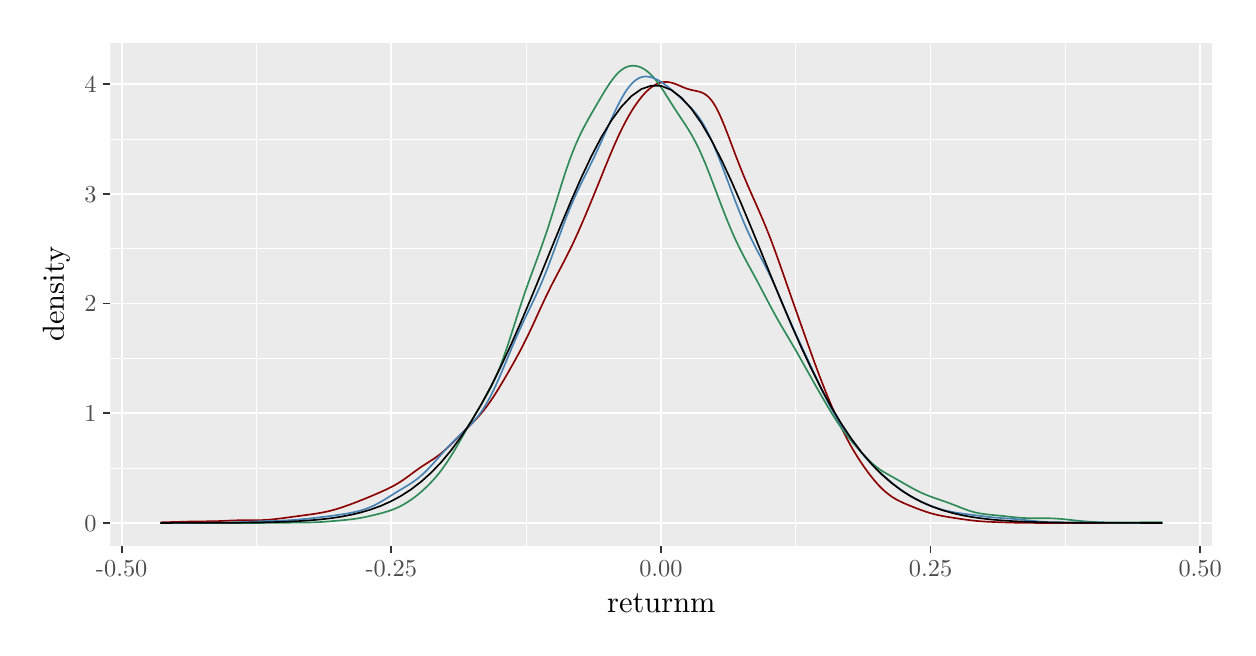
\begin{tikzpicture}[x=1pt,y=1pt]
\definecolor{fillColor}{RGB}{255,255,255}
\path[use as bounding box,fill=fillColor,fill opacity=0.00] (0,0) rectangle (433.62,216.81);
\begin{scope}
\path[clip] (  0.00,  0.00) rectangle (433.62,216.81);
\definecolor{drawColor}{RGB}{255,255,255}
\definecolor{fillColor}{RGB}{255,255,255}

\path[draw=drawColor,line width= 0.6pt,line join=round,line cap=round,fill=fillColor] (  0.00,  0.00) rectangle (433.62,216.81);
\end{scope}
\begin{scope}
\path[clip] ( 29.87, 29.59) rectangle (428.12,211.31);
\definecolor{fillColor}{gray}{0.92}

\path[fill=fillColor] ( 29.87, 29.59) rectangle (428.12,211.31);
\definecolor{drawColor}{RGB}{255,255,255}

\path[draw=drawColor,line width= 0.3pt,line join=round] ( 29.87, 57.67) --
	(428.12, 57.67);

\path[draw=drawColor,line width= 0.3pt,line join=round] ( 29.87, 97.30) --
	(428.12, 97.30);

\path[draw=drawColor,line width= 0.3pt,line join=round] ( 29.87,136.94) --
	(428.12,136.94);

\path[draw=drawColor,line width= 0.3pt,line join=round] ( 29.87,176.58) --
	(428.12,176.58);

\path[draw=drawColor,line width= 0.3pt,line join=round] ( 82.68, 29.59) --
	( 82.68,211.31);

\path[draw=drawColor,line width= 0.3pt,line join=round] (180.11, 29.59) --
	(180.11,211.31);

\path[draw=drawColor,line width= 0.3pt,line join=round] (277.54, 29.59) --
	(277.54,211.31);

\path[draw=drawColor,line width= 0.3pt,line join=round] (374.97, 29.59) --
	(374.97,211.31);

\path[draw=drawColor,line width= 0.6pt,line join=round] ( 29.87, 37.85) --
	(428.12, 37.85);

\path[draw=drawColor,line width= 0.6pt,line join=round] ( 29.87, 77.49) --
	(428.12, 77.49);

\path[draw=drawColor,line width= 0.6pt,line join=round] ( 29.87,117.12) --
	(428.12,117.12);

\path[draw=drawColor,line width= 0.6pt,line join=round] ( 29.87,156.76) --
	(428.12,156.76);

\path[draw=drawColor,line width= 0.6pt,line join=round] ( 29.87,196.40) --
	(428.12,196.40);

\path[draw=drawColor,line width= 0.6pt,line join=round] ( 33.97, 29.59) --
	( 33.97,211.31);

\path[draw=drawColor,line width= 0.6pt,line join=round] (131.40, 29.59) --
	(131.40,211.31);

\path[draw=drawColor,line width= 0.6pt,line join=round] (228.83, 29.59) --
	(228.83,211.31);

\path[draw=drawColor,line width= 0.6pt,line join=round] (326.26, 29.59) --
	(326.26,211.31);

\path[draw=drawColor,line width= 0.6pt,line join=round] (423.69, 29.59) --
	(423.69,211.31);
\definecolor{drawColor}{RGB}{139,0,0}

\path[draw=drawColor,line width= 0.6pt,line join=round] ( 47.97, 38.05) --
	( 48.68, 38.07) --
	( 49.39, 38.09) --
	( 50.10, 38.11) --
	( 50.81, 38.13) --
	( 51.51, 38.15) --
	( 52.22, 38.17) --
	( 52.93, 38.19) --
	( 53.64, 38.21) --
	( 54.35, 38.23) --
	( 55.06, 38.25) --
	( 55.76, 38.27) --
	( 56.47, 38.29) --
	( 57.18, 38.31) --
	( 57.89, 38.33) --
	( 58.60, 38.35) --
	( 59.31, 38.36) --
	( 60.02, 38.37) --
	( 60.72, 38.39) --
	( 61.43, 38.40) --
	( 62.14, 38.40) --
	( 62.85, 38.41) --
	( 63.56, 38.42) --
	( 64.27, 38.42) --
	( 64.98, 38.43) --
	( 65.68, 38.44) --
	( 66.39, 38.45) --
	( 67.10, 38.46) --
	( 67.81, 38.48) --
	( 68.52, 38.50) --
	( 69.23, 38.52) --
	( 69.93, 38.55) --
	( 70.64, 38.58) --
	( 71.35, 38.61) --
	( 72.06, 38.65) --
	( 72.77, 38.68) --
	( 73.48, 38.72) --
	( 74.19, 38.74) --
	( 74.89, 38.77) --
	( 75.60, 38.79) --
	( 76.31, 38.81) --
	( 77.02, 38.82) --
	( 77.73, 38.82) --
	( 78.44, 38.82) --
	( 79.15, 38.82) --
	( 79.85, 38.82) --
	( 80.56, 38.81) --
	( 81.27, 38.81) --
	( 81.98, 38.81) --
	( 82.69, 38.82) --
	( 83.40, 38.83) --
	( 84.10, 38.85) --
	( 84.81, 38.87) --
	( 85.52, 38.91) --
	( 86.23, 38.95) --
	( 86.94, 39.00) --
	( 87.65, 39.06) --
	( 88.36, 39.13) --
	( 89.06, 39.20) --
	( 89.77, 39.28) --
	( 90.48, 39.37) --
	( 91.19, 39.45) --
	( 91.90, 39.54) --
	( 92.61, 39.63) --
	( 93.32, 39.73) --
	( 94.02, 39.82) --
	( 94.73, 39.92) --
	( 95.44, 40.02) --
	( 96.15, 40.11) --
	( 96.86, 40.21) --
	( 97.57, 40.30) --
	( 98.28, 40.40) --
	( 98.98, 40.49) --
	( 99.69, 40.59) --
	(100.40, 40.68) --
	(101.11, 40.78) --
	(101.82, 40.87) --
	(102.53, 40.97) --
	(103.23, 41.07) --
	(103.94, 41.18) --
	(104.65, 41.29) --
	(105.36, 41.41) --
	(106.07, 41.53) --
	(106.78, 41.67) --
	(107.49, 41.81) --
	(108.19, 41.96) --
	(108.90, 42.13) --
	(109.61, 42.31) --
	(110.32, 42.49) --
	(111.03, 42.69) --
	(111.74, 42.90) --
	(112.45, 43.12) --
	(113.15, 43.35) --
	(113.86, 43.58) --
	(114.57, 43.83) --
	(115.28, 44.08) --
	(115.99, 44.33) --
	(116.70, 44.59) --
	(117.40, 44.85) --
	(118.11, 45.12) --
	(118.82, 45.39) --
	(119.53, 45.67) --
	(120.24, 45.95) --
	(120.95, 46.23) --
	(121.66, 46.51) --
	(122.36, 46.80) --
	(123.07, 47.10) --
	(123.78, 47.39) --
	(124.49, 47.69) --
	(125.20, 48.00) --
	(125.91, 48.30) --
	(126.62, 48.61) --
	(127.32, 48.92) --
	(128.03, 49.23) --
	(128.74, 49.55) --
	(129.45, 49.88) --
	(130.16, 50.21) --
	(130.87, 50.56) --
	(131.57, 50.92) --
	(132.28, 51.30) --
	(132.99, 51.69) --
	(133.70, 52.11) --
	(134.41, 52.55) --
	(135.12, 53.01) --
	(135.83, 53.49) --
	(136.53, 53.98) --
	(137.24, 54.49) --
	(137.95, 55.01) --
	(138.66, 55.54) --
	(139.37, 56.06) --
	(140.08, 56.58) --
	(140.79, 57.09) --
	(141.49, 57.59) --
	(142.20, 58.08) --
	(142.91, 58.55) --
	(143.62, 59.02) --
	(144.33, 59.47) --
	(145.04, 59.92) --
	(145.74, 60.38) --
	(146.45, 60.84) --
	(147.16, 61.32) --
	(147.87, 61.83) --
	(148.58, 62.35) --
	(149.29, 62.91) --
	(150.00, 63.49) --
	(150.70, 64.10) --
	(151.41, 64.74) --
	(152.12, 65.40) --
	(152.83, 66.09) --
	(153.54, 66.78) --
	(154.25, 67.49) --
	(154.96, 68.20) --
	(155.66, 68.92) --
	(156.37, 69.63) --
	(157.08, 70.34) --
	(157.79, 71.05) --
	(158.50, 71.76) --
	(159.21, 72.46) --
	(159.92, 73.17) --
	(160.62, 73.89) --
	(161.33, 74.62) --
	(162.04, 75.37) --
	(162.75, 76.14) --
	(163.46, 76.94) --
	(164.17, 77.77) --
	(164.87, 78.64) --
	(165.58, 79.56) --
	(166.29, 80.51) --
	(167.00, 81.51) --
	(167.71, 82.54) --
	(168.42, 83.61) --
	(169.13, 84.72) --
	(169.83, 85.85) --
	(170.54, 87.01) --
	(171.25, 88.20) --
	(171.96, 89.39) --
	(172.67, 90.60) --
	(173.38, 91.82) --
	(174.09, 93.05) --
	(174.79, 94.30) --
	(175.50, 95.55) --
	(176.21, 96.82) --
	(176.92, 98.11) --
	(177.63, 99.43) --
	(178.34,100.77) --
	(179.04,102.15) --
	(179.75,103.55) --
	(180.46,104.99) --
	(181.17,106.46) --
	(181.88,107.96) --
	(182.59,109.48) --
	(183.30,111.02) --
	(184.00,112.57) --
	(184.71,114.12) --
	(185.42,115.66) --
	(186.13,117.19) --
	(186.84,118.70) --
	(187.55,120.18) --
	(188.26,121.63) --
	(188.96,123.06) --
	(189.67,124.46) --
	(190.38,125.83) --
	(191.09,127.18) --
	(191.80,128.53) --
	(192.51,129.87) --
	(193.21,131.22) --
	(193.92,132.57) --
	(194.63,133.95) --
	(195.34,135.36) --
	(196.05,136.79) --
	(196.76,138.26) --
	(197.47,139.77) --
	(198.17,141.31) --
	(198.88,142.88) --
	(199.59,144.49) --
	(200.30,146.11) --
	(201.01,147.77) --
	(201.72,149.44) --
	(202.43,151.13) --
	(203.13,152.83) --
	(203.84,154.54) --
	(204.55,156.27) --
	(205.26,158.01) --
	(205.97,159.75) --
	(206.68,161.50) --
	(207.39,163.25) --
	(208.09,165.00) --
	(208.80,166.75) --
	(209.51,168.48) --
	(210.22,170.20) --
	(210.93,171.89) --
	(211.64,173.54) --
	(212.34,175.16) --
	(213.05,176.74) --
	(213.76,178.27) --
	(214.47,179.75) --
	(215.18,181.18) --
	(215.89,182.55) --
	(216.60,183.86) --
	(217.30,185.11) --
	(218.01,186.31) --
	(218.72,187.45) --
	(219.43,188.54) --
	(220.14,189.57) --
	(220.85,190.54) --
	(221.56,191.45) --
	(222.26,192.30) --
	(222.97,193.09) --
	(223.68,193.80) --
	(224.39,194.46) --
	(225.10,195.05) --
	(225.81,195.57) --
	(226.51,196.02) --
	(227.22,196.40) --
	(227.93,196.70) --
	(228.64,196.94) --
	(229.35,197.10) --
	(230.06,197.18) --
	(230.77,197.19) --
	(231.47,197.14) --
	(232.18,197.02) --
	(232.89,196.84) --
	(233.60,196.62) --
	(234.31,196.36) --
	(235.02,196.07) --
	(235.73,195.76) --
	(236.43,195.46) --
	(237.14,195.17) --
	(237.85,194.90) --
	(238.56,194.66) --
	(239.27,194.45) --
	(239.98,194.27) --
	(240.68,194.12) --
	(241.39,193.97) --
	(242.10,193.82) --
	(242.81,193.64) --
	(243.52,193.40) --
	(244.23,193.08) --
	(244.94,192.65) --
	(245.64,192.11) --
	(246.35,191.43) --
	(247.06,190.59) --
	(247.77,189.60) --
	(248.48,188.46) --
	(249.19,187.14) --
	(249.90,185.69) --
	(250.60,184.12) --
	(251.31,182.44) --
	(252.02,180.68) --
	(252.73,178.86) --
	(253.44,177.00) --
	(254.15,175.12) --
	(254.85,173.23) --
	(255.56,171.35) --
	(256.27,169.49) --
	(256.98,167.66) --
	(257.69,165.87) --
	(258.40,164.11) --
	(259.11,162.39) --
	(259.81,160.71) --
	(260.52,159.06) --
	(261.23,157.44) --
	(261.94,155.84) --
	(262.65,154.24) --
	(263.36,152.65) --
	(264.07,151.05) --
	(264.77,149.42) --
	(265.48,147.78) --
	(266.19,146.09) --
	(266.90,144.37) --
	(267.61,142.60) --
	(268.32,140.79) --
	(269.03,138.92) --
	(269.73,137.02) --
	(270.44,135.08) --
	(271.15,133.10) --
	(271.86,131.10) --
	(272.57,129.09) --
	(273.28,127.06) --
	(273.98,125.03) --
	(274.69,122.99) --
	(275.40,120.96) --
	(276.11,118.93) --
	(276.82,116.91) --
	(277.53,114.90) --
	(278.24,112.89) --
	(278.94,110.89) --
	(279.65,108.88) --
	(280.36,106.88) --
	(281.07,104.88) --
	(281.78,102.89) --
	(282.49,100.91) --
	(283.20, 98.93) --
	(283.90, 96.97) --
	(284.61, 95.03) --
	(285.32, 93.12) --
	(286.03, 91.23) --
	(286.74, 89.37) --
	(287.45, 87.55) --
	(288.15, 85.76) --
	(288.86, 84.02) --
	(289.57, 82.30) --
	(290.28, 80.62) --
	(290.99, 78.97) --
	(291.70, 77.36) --
	(292.41, 75.78) --
	(293.11, 74.24) --
	(293.82, 72.74) --
	(294.53, 71.28) --
	(295.24, 69.86) --
	(295.95, 68.48) --
	(296.66, 67.15) --
	(297.37, 65.86) --
	(298.07, 64.62) --
	(298.78, 63.42) --
	(299.49, 62.26) --
	(300.20, 61.13) --
	(300.91, 60.05) --
	(301.62, 59.00) --
	(302.32, 57.98) --
	(303.03, 56.99) --
	(303.74, 56.02) --
	(304.45, 55.09) --
	(305.16, 54.19) --
	(305.87, 53.32) --
	(306.58, 52.49) --
	(307.28, 51.70) --
	(307.99, 50.95) --
	(308.70, 50.24) --
	(309.41, 49.57) --
	(310.12, 48.96) --
	(310.83, 48.38) --
	(311.54, 47.84) --
	(312.24, 47.35) --
	(312.95, 46.89) --
	(313.66, 46.47) --
	(314.37, 46.08) --
	(315.08, 45.72) --
	(315.79, 45.38) --
	(316.49, 45.05) --
	(317.20, 44.74) --
	(317.91, 44.44) --
	(318.62, 44.15) --
	(319.33, 43.86) --
	(320.04, 43.58) --
	(320.75, 43.30) --
	(321.45, 43.03) --
	(322.16, 42.76) --
	(322.87, 42.50) --
	(323.58, 42.25) --
	(324.29, 42.00) --
	(325.00, 41.77) --
	(325.71, 41.55) --
	(326.41, 41.33) --
	(327.12, 41.14) --
	(327.83, 40.95) --
	(328.54, 40.78) --
	(329.25, 40.63) --
	(329.96, 40.48) --
	(330.67, 40.34) --
	(331.37, 40.21) --
	(332.08, 40.09) --
	(332.79, 39.97) --
	(333.50, 39.85) --
	(334.21, 39.74) --
	(334.92, 39.63) --
	(335.62, 39.53) --
	(336.33, 39.42) --
	(337.04, 39.31) --
	(337.75, 39.21) --
	(338.46, 39.11) --
	(339.17, 39.01) --
	(339.88, 38.92) --
	(340.58, 38.83) --
	(341.29, 38.74) --
	(342.00, 38.66) --
	(342.71, 38.59) --
	(343.42, 38.52) --
	(344.13, 38.46) --
	(344.84, 38.41) --
	(345.54, 38.36) --
	(346.25, 38.32) --
	(346.96, 38.28) --
	(347.67, 38.24) --
	(348.38, 38.21) --
	(349.09, 38.18) --
	(349.79, 38.15) --
	(350.50, 38.13) --
	(351.21, 38.10) --
	(351.92, 38.08) --
	(352.63, 38.05) --
	(353.34, 38.03) --
	(354.05, 38.01) --
	(354.75, 37.99) --
	(355.46, 37.97) --
	(356.17, 37.95) --
	(356.88, 37.93) --
	(357.59, 37.92) --
	(358.30, 37.91) --
	(359.01, 37.89) --
	(359.71, 37.88) --
	(360.42, 37.88) --
	(361.13, 37.87) --
	(361.84, 37.86) --
	(362.55, 37.86) --
	(363.26, 37.86) --
	(363.96, 37.85) --
	(364.67, 37.85) --
	(365.38, 37.85) --
	(366.09, 37.85) --
	(366.80, 37.85) --
	(367.51, 37.85) --
	(368.22, 37.85) --
	(368.92, 37.85) --
	(369.63, 37.85) --
	(370.34, 37.85) --
	(371.05, 37.85) --
	(371.76, 37.85) --
	(372.47, 37.85) --
	(373.18, 37.85) --
	(373.88, 37.85) --
	(374.59, 37.85) --
	(375.30, 37.85) --
	(376.01, 37.85) --
	(376.72, 37.85) --
	(377.43, 37.85) --
	(378.13, 37.85) --
	(378.84, 37.85) --
	(379.55, 37.85) --
	(380.26, 37.85) --
	(380.97, 37.85) --
	(381.68, 37.85) --
	(382.39, 37.85) --
	(383.09, 37.85) --
	(383.80, 37.85) --
	(384.51, 37.85) --
	(385.22, 37.85) --
	(385.93, 37.85) --
	(386.64, 37.85) --
	(387.35, 37.85) --
	(388.05, 37.85) --
	(388.76, 37.85) --
	(389.47, 37.85) --
	(390.18, 37.85) --
	(390.89, 37.85) --
	(391.60, 37.85) --
	(392.31, 37.85) --
	(393.01, 37.85) --
	(393.72, 37.85) --
	(394.43, 37.85) --
	(395.14, 37.85) --
	(395.85, 37.85) --
	(396.56, 37.85) --
	(397.26, 37.85) --
	(397.97, 37.85) --
	(398.68, 37.85) --
	(399.39, 37.85) --
	(400.10, 37.85) --
	(400.81, 37.85) --
	(401.52, 37.85) --
	(402.22, 37.85) --
	(402.93, 37.85) --
	(403.64, 37.85) --
	(404.35, 37.85) --
	(405.06, 37.85) --
	(405.77, 37.85) --
	(406.48, 37.85) --
	(407.18, 37.85) --
	(407.89, 37.85) --
	(408.60, 37.85) --
	(409.31, 37.85) --
	(410.02, 37.85);
\definecolor{drawColor}{RGB}{46,139,87}

\path[draw=drawColor,line width= 0.6pt,line join=round] ( 47.97, 37.85) --
	( 48.68, 37.85) --
	( 49.39, 37.85) --
	( 50.10, 37.85) --
	( 50.81, 37.85) --
	( 51.51, 37.85) --
	( 52.22, 37.85) --
	( 52.93, 37.85) --
	( 53.64, 37.85) --
	( 54.35, 37.85) --
	( 55.06, 37.85) --
	( 55.76, 37.85) --
	( 56.47, 37.85) --
	( 57.18, 37.85) --
	( 57.89, 37.85) --
	( 58.60, 37.85) --
	( 59.31, 37.85) --
	( 60.02, 37.85) --
	( 60.72, 37.85) --
	( 61.43, 37.85) --
	( 62.14, 37.85) --
	( 62.85, 37.85) --
	( 63.56, 37.85) --
	( 64.27, 37.85) --
	( 64.98, 37.85) --
	( 65.68, 37.85) --
	( 66.39, 37.85) --
	( 67.10, 37.85) --
	( 67.81, 37.85) --
	( 68.52, 37.85) --
	( 69.23, 37.85) --
	( 69.93, 37.85) --
	( 70.64, 37.85) --
	( 71.35, 37.85) --
	( 72.06, 37.85) --
	( 72.77, 37.85) --
	( 73.48, 37.85) --
	( 74.19, 37.85) --
	( 74.89, 37.85) --
	( 75.60, 37.85) --
	( 76.31, 37.85) --
	( 77.02, 37.85) --
	( 77.73, 37.85) --
	( 78.44, 37.85) --
	( 79.15, 37.85) --
	( 79.85, 37.85) --
	( 80.56, 37.85) --
	( 81.27, 37.85) --
	( 81.98, 37.85) --
	( 82.69, 37.85) --
	( 83.40, 37.85) --
	( 84.10, 37.85) --
	( 84.81, 37.85) --
	( 85.52, 37.85) --
	( 86.23, 37.86) --
	( 86.94, 37.86) --
	( 87.65, 37.87) --
	( 88.36, 37.87) --
	( 89.06, 37.88) --
	( 89.77, 37.88) --
	( 90.48, 37.89) --
	( 91.19, 37.90) --
	( 91.90, 37.91) --
	( 92.61, 37.92) --
	( 93.32, 37.92) --
	( 94.02, 37.93) --
	( 94.73, 37.94) --
	( 95.44, 37.95) --
	( 96.15, 37.96) --
	( 96.86, 37.97) --
	( 97.57, 37.97) --
	( 98.28, 37.98) --
	( 98.98, 37.99) --
	( 99.69, 37.99) --
	(100.40, 38.00) --
	(101.11, 38.01) --
	(101.82, 38.02) --
	(102.53, 38.04) --
	(103.23, 38.06) --
	(103.94, 38.08) --
	(104.65, 38.11) --
	(105.36, 38.15) --
	(106.07, 38.19) --
	(106.78, 38.23) --
	(107.49, 38.28) --
	(108.19, 38.34) --
	(108.90, 38.40) --
	(109.61, 38.46) --
	(110.32, 38.52) --
	(111.03, 38.58) --
	(111.74, 38.65) --
	(112.45, 38.71) --
	(113.15, 38.77) --
	(113.86, 38.84) --
	(114.57, 38.90) --
	(115.28, 38.97) --
	(115.99, 39.05) --
	(116.70, 39.13) --
	(117.40, 39.21) --
	(118.11, 39.31) --
	(118.82, 39.41) --
	(119.53, 39.53) --
	(120.24, 39.65) --
	(120.95, 39.78) --
	(121.66, 39.92) --
	(122.36, 40.07) --
	(123.07, 40.23) --
	(123.78, 40.39) --
	(124.49, 40.55) --
	(125.20, 40.72) --
	(125.91, 40.89) --
	(126.62, 41.07) --
	(127.32, 41.25) --
	(128.03, 41.44) --
	(128.74, 41.64) --
	(129.45, 41.84) --
	(130.16, 42.06) --
	(130.87, 42.30) --
	(131.57, 42.55) --
	(132.28, 42.82) --
	(132.99, 43.11) --
	(133.70, 43.42) --
	(134.41, 43.76) --
	(135.12, 44.12) --
	(135.83, 44.51) --
	(136.53, 44.92) --
	(137.24, 45.36) --
	(137.95, 45.82) --
	(138.66, 46.31) --
	(139.37, 46.82) --
	(140.08, 47.35) --
	(140.79, 47.91) --
	(141.49, 48.49) --
	(142.20, 49.10) --
	(142.91, 49.72) --
	(143.62, 50.38) --
	(144.33, 51.06) --
	(145.04, 51.76) --
	(145.74, 52.50) --
	(146.45, 53.26) --
	(147.16, 54.05) --
	(147.87, 54.89) --
	(148.58, 55.75) --
	(149.29, 56.66) --
	(150.00, 57.60) --
	(150.70, 58.60) --
	(151.41, 59.63) --
	(152.12, 60.70) --
	(152.83, 61.81) --
	(153.54, 62.95) --
	(154.25, 64.12) --
	(154.96, 65.32) --
	(155.66, 66.54) --
	(156.37, 67.77) --
	(157.08, 69.01) --
	(157.79, 70.26) --
	(158.50, 71.50) --
	(159.21, 72.73) --
	(159.92, 73.96) --
	(160.62, 75.17) --
	(161.33, 76.38) --
	(162.04, 77.57) --
	(162.75, 78.75) --
	(163.46, 79.93) --
	(164.17, 81.11) --
	(164.87, 82.31) --
	(165.58, 83.54) --
	(166.29, 84.81) --
	(167.00, 86.14) --
	(167.71, 87.52) --
	(168.42, 88.99) --
	(169.13, 90.53) --
	(169.83, 92.18) --
	(170.54, 93.93) --
	(171.25, 95.77) --
	(171.96, 97.70) --
	(172.67, 99.72) --
	(173.38,101.80) --
	(174.09,103.94) --
	(174.79,106.13) --
	(175.50,108.34) --
	(176.21,110.56) --
	(176.92,112.77) --
	(177.63,114.96) --
	(178.34,117.11) --
	(179.04,119.23) --
	(179.75,121.30) --
	(180.46,123.33) --
	(181.17,125.32) --
	(181.88,127.28) --
	(182.59,129.21) --
	(183.30,131.13) --
	(184.00,133.05) --
	(184.71,134.99) --
	(185.42,136.96) --
	(186.13,138.97) --
	(186.84,141.02) --
	(187.55,143.12) --
	(188.26,145.28) --
	(188.96,147.48) --
	(189.67,149.73) --
	(190.38,152.02) --
	(191.09,154.32) --
	(191.80,156.62) --
	(192.51,158.90) --
	(193.21,161.16) --
	(193.92,163.36) --
	(194.63,165.51) --
	(195.34,167.57) --
	(196.05,169.56) --
	(196.76,171.43) --
	(197.47,173.22) --
	(198.17,174.90) --
	(198.88,176.50) --
	(199.59,178.02) --
	(200.30,179.47) --
	(201.01,180.85) --
	(201.72,182.17) --
	(202.43,183.46) --
	(203.13,184.72) --
	(203.84,185.96) --
	(204.55,187.18) --
	(205.26,188.40) --
	(205.97,189.62) --
	(206.68,190.83) --
	(207.39,192.02) --
	(208.09,193.20) --
	(208.80,194.36) --
	(209.51,195.48) --
	(210.22,196.55) --
	(210.93,197.56) --
	(211.64,198.51) --
	(212.34,199.37) --
	(213.05,200.16) --
	(213.76,200.85) --
	(214.47,201.45) --
	(215.18,201.96) --
	(215.89,202.36) --
	(216.60,202.67) --
	(217.30,202.88) --
	(218.01,203.01) --
	(218.72,203.05) --
	(219.43,203.01) --
	(220.14,202.90) --
	(220.85,202.71) --
	(221.56,202.45) --
	(222.26,202.11) --
	(222.97,201.69) --
	(223.68,201.19) --
	(224.39,200.61) --
	(225.10,199.95) --
	(225.81,199.22) --
	(226.51,198.42) --
	(227.22,197.54) --
	(227.93,196.60) --
	(228.64,195.60) --
	(229.35,194.55) --
	(230.06,193.46) --
	(230.77,192.35) --
	(231.47,191.23) --
	(232.18,190.10) --
	(232.89,188.98) --
	(233.60,187.87) --
	(234.31,186.77) --
	(235.02,185.70) --
	(235.73,184.63) --
	(236.43,183.57) --
	(237.14,182.50) --
	(237.85,181.42) --
	(238.56,180.31) --
	(239.27,179.15) --
	(239.98,177.95) --
	(240.68,176.68) --
	(241.39,175.35) --
	(242.10,173.93) --
	(242.81,172.44) --
	(243.52,170.86) --
	(244.23,169.22) --
	(244.94,167.52) --
	(245.64,165.76) --
	(246.35,163.95) --
	(247.06,162.11) --
	(247.77,160.25) --
	(248.48,158.36) --
	(249.19,156.48) --
	(249.90,154.60) --
	(250.60,152.73) --
	(251.31,150.89) --
	(252.02,149.08) --
	(252.73,147.30) --
	(253.44,145.57) --
	(254.15,143.88) --
	(254.85,142.25) --
	(255.56,140.68) --
	(256.27,139.16) --
	(256.98,137.69) --
	(257.69,136.27) --
	(258.40,134.89) --
	(259.11,133.54) --
	(259.81,132.21) --
	(260.52,130.91) --
	(261.23,129.61) --
	(261.94,128.31) --
	(262.65,127.01) --
	(263.36,125.69) --
	(264.07,124.37) --
	(264.77,123.03) --
	(265.48,121.68) --
	(266.19,120.33) --
	(266.90,118.98) --
	(267.61,117.63) --
	(268.32,116.29) --
	(269.03,114.97) --
	(269.73,113.67) --
	(270.44,112.39) --
	(271.15,111.13) --
	(271.86,109.89) --
	(272.57,108.67) --
	(273.28,107.47) --
	(273.98,106.27) --
	(274.69,105.08) --
	(275.40,103.88) --
	(276.11,102.68) --
	(276.82,101.47) --
	(277.53,100.25) --
	(278.24, 99.01) --
	(278.94, 97.76) --
	(279.65, 96.51) --
	(280.36, 95.24) --
	(281.07, 93.97) --
	(281.78, 92.70) --
	(282.49, 91.44) --
	(283.20, 90.17) --
	(283.90, 88.91) --
	(284.61, 87.66) --
	(285.32, 86.41) --
	(286.03, 85.17) --
	(286.74, 83.94) --
	(287.45, 82.71) --
	(288.15, 81.50) --
	(288.86, 80.30) --
	(289.57, 79.11) --
	(290.28, 77.94) --
	(290.99, 76.79) --
	(291.70, 75.67) --
	(292.41, 74.58) --
	(293.11, 73.52) --
	(293.82, 72.49) --
	(294.53, 71.49) --
	(295.24, 70.53) --
	(295.95, 69.60) --
	(296.66, 68.69) --
	(297.37, 67.81) --
	(298.07, 66.96) --
	(298.78, 66.12) --
	(299.49, 65.29) --
	(300.20, 64.48) --
	(300.91, 63.69) --
	(301.62, 62.91) --
	(302.32, 62.15) --
	(303.03, 61.42) --
	(303.74, 60.71) --
	(304.45, 60.03) --
	(305.16, 59.38) --
	(305.87, 58.77) --
	(306.58, 58.19) --
	(307.28, 57.66) --
	(307.99, 57.15) --
	(308.70, 56.68) --
	(309.41, 56.24) --
	(310.12, 55.81) --
	(310.83, 55.41) --
	(311.54, 55.01) --
	(312.24, 54.61) --
	(312.95, 54.22) --
	(313.66, 53.82) --
	(314.37, 53.42) --
	(315.08, 53.02) --
	(315.79, 52.61) --
	(316.49, 52.20) --
	(317.20, 51.79) --
	(317.91, 51.38) --
	(318.62, 50.98) --
	(319.33, 50.58) --
	(320.04, 50.20) --
	(320.75, 49.82) --
	(321.45, 49.46) --
	(322.16, 49.11) --
	(322.87, 48.78) --
	(323.58, 48.46) --
	(324.29, 48.16) --
	(325.00, 47.87) --
	(325.71, 47.59) --
	(326.41, 47.32) --
	(327.12, 47.06) --
	(327.83, 46.81) --
	(328.54, 46.56) --
	(329.25, 46.32) --
	(329.96, 46.08) --
	(330.67, 45.83) --
	(331.37, 45.59) --
	(332.08, 45.34) --
	(332.79, 45.08) --
	(333.50, 44.82) --
	(334.21, 44.55) --
	(334.92, 44.27) --
	(335.62, 43.99) --
	(336.33, 43.71) --
	(337.04, 43.43) --
	(337.75, 43.16) --
	(338.46, 42.89) --
	(339.17, 42.63) --
	(339.88, 42.38) --
	(340.58, 42.15) --
	(341.29, 41.94) --
	(342.00, 41.75) --
	(342.71, 41.58) --
	(343.42, 41.43) --
	(344.13, 41.29) --
	(344.84, 41.17) --
	(345.54, 41.07) --
	(346.25, 40.98) --
	(346.96, 40.90) --
	(347.67, 40.82) --
	(348.38, 40.75) --
	(349.09, 40.69) --
	(349.79, 40.62) --
	(350.50, 40.55) --
	(351.21, 40.48) --
	(351.92, 40.41) --
	(352.63, 40.34) --
	(353.34, 40.26) --
	(354.05, 40.18) --
	(354.75, 40.10) --
	(355.46, 40.02) --
	(356.17, 39.94) --
	(356.88, 39.87) --
	(357.59, 39.80) --
	(358.30, 39.74) --
	(359.01, 39.69) --
	(359.71, 39.64) --
	(360.42, 39.61) --
	(361.13, 39.58) --
	(361.84, 39.56) --
	(362.55, 39.55) --
	(363.26, 39.54) --
	(363.96, 39.54) --
	(364.67, 39.54) --
	(365.38, 39.54) --
	(366.09, 39.55) --
	(366.80, 39.55) --
	(367.51, 39.55) --
	(368.22, 39.54) --
	(368.92, 39.53) --
	(369.63, 39.51) --
	(370.34, 39.49) --
	(371.05, 39.45) --
	(371.76, 39.41) --
	(372.47, 39.36) --
	(373.18, 39.31) --
	(373.88, 39.25) --
	(374.59, 39.18) --
	(375.30, 39.10) --
	(376.01, 39.03) --
	(376.72, 38.95) --
	(377.43, 38.87) --
	(378.13, 38.79) --
	(378.84, 38.71) --
	(379.55, 38.64) --
	(380.26, 38.57) --
	(380.97, 38.50) --
	(381.68, 38.44) --
	(382.39, 38.38) --
	(383.09, 38.33) --
	(383.80, 38.28) --
	(384.51, 38.24) --
	(385.22, 38.20) --
	(385.93, 38.17) --
	(386.64, 38.14) --
	(387.35, 38.11) --
	(388.05, 38.09) --
	(388.76, 38.07) --
	(389.47, 38.05) --
	(390.18, 38.04) --
	(390.89, 38.02) --
	(391.60, 38.01) --
	(392.31, 38.01) --
	(393.01, 38.00) --
	(393.72, 38.00) --
	(394.43, 38.00) --
	(395.14, 38.00) --
	(395.85, 38.00) --
	(396.56, 38.01) --
	(397.26, 38.01) --
	(397.97, 38.02) --
	(398.68, 38.03) --
	(399.39, 38.04) --
	(400.10, 38.05) --
	(400.81, 38.05) --
	(401.52, 38.06) --
	(402.22, 38.07) --
	(402.93, 38.08) --
	(403.64, 38.09) --
	(404.35, 38.09) --
	(405.06, 38.10) --
	(405.77, 38.10) --
	(406.48, 38.10) --
	(407.18, 38.10) --
	(407.89, 38.09) --
	(408.60, 38.09) --
	(409.31, 38.08) --
	(410.02, 38.07);
\definecolor{drawColor}{RGB}{70,130,180}

\path[draw=drawColor,line width= 0.6pt,line join=round] ( 47.97, 37.85) --
	( 48.68, 37.85) --
	( 49.39, 37.85) --
	( 50.10, 37.85) --
	( 50.81, 37.85) --
	( 51.51, 37.85) --
	( 52.22, 37.85) --
	( 52.93, 37.85) --
	( 53.64, 37.85) --
	( 54.35, 37.85) --
	( 55.06, 37.85) --
	( 55.76, 37.85) --
	( 56.47, 37.85) --
	( 57.18, 37.85) --
	( 57.89, 37.85) --
	( 58.60, 37.85) --
	( 59.31, 37.85) --
	( 60.02, 37.86) --
	( 60.72, 37.86) --
	( 61.43, 37.86) --
	( 62.14, 37.87) --
	( 62.85, 37.87) --
	( 63.56, 37.88) --
	( 64.27, 37.89) --
	( 64.98, 37.90) --
	( 65.68, 37.91) --
	( 66.39, 37.92) --
	( 67.10, 37.93) --
	( 67.81, 37.94) --
	( 68.52, 37.95) --
	( 69.23, 37.96) --
	( 69.93, 37.97) --
	( 70.64, 37.99) --
	( 71.35, 38.00) --
	( 72.06, 38.01) --
	( 72.77, 38.03) --
	( 73.48, 38.04) --
	( 74.19, 38.06) --
	( 74.89, 38.08) --
	( 75.60, 38.10) --
	( 76.31, 38.12) --
	( 77.02, 38.15) --
	( 77.73, 38.18) --
	( 78.44, 38.21) --
	( 79.15, 38.24) --
	( 79.85, 38.27) --
	( 80.56, 38.31) --
	( 81.27, 38.34) --
	( 81.98, 38.37) --
	( 82.69, 38.40) --
	( 83.40, 38.43) --
	( 84.10, 38.46) --
	( 84.81, 38.49) --
	( 85.52, 38.51) --
	( 86.23, 38.53) --
	( 86.94, 38.55) --
	( 87.65, 38.57) --
	( 88.36, 38.58) --
	( 89.06, 38.60) --
	( 89.77, 38.62) --
	( 90.48, 38.64) --
	( 91.19, 38.66) --
	( 91.90, 38.69) --
	( 92.61, 38.72) --
	( 93.32, 38.75) --
	( 94.02, 38.79) --
	( 94.73, 38.83) --
	( 95.44, 38.88) --
	( 96.15, 38.93) --
	( 96.86, 38.99) --
	( 97.57, 39.04) --
	( 98.28, 39.11) --
	( 98.98, 39.17) --
	( 99.69, 39.24) --
	(100.40, 39.31) --
	(101.11, 39.38) --
	(101.82, 39.45) --
	(102.53, 39.53) --
	(103.23, 39.61) --
	(103.94, 39.69) --
	(104.65, 39.77) --
	(105.36, 39.85) --
	(106.07, 39.94) --
	(106.78, 40.03) --
	(107.49, 40.11) --
	(108.19, 40.20) --
	(108.90, 40.30) --
	(109.61, 40.39) --
	(110.32, 40.48) --
	(111.03, 40.58) --
	(111.74, 40.68) --
	(112.45, 40.78) --
	(113.15, 40.88) --
	(113.86, 40.99) --
	(114.57, 41.10) --
	(115.28, 41.22) --
	(115.99, 41.35) --
	(116.70, 41.49) --
	(117.40, 41.63) --
	(118.11, 41.78) --
	(118.82, 41.95) --
	(119.53, 42.13) --
	(120.24, 42.32) --
	(120.95, 42.53) --
	(121.66, 42.76) --
	(122.36, 43.00) --
	(123.07, 43.27) --
	(123.78, 43.55) --
	(124.49, 43.86) --
	(125.20, 44.19) --
	(125.91, 44.55) --
	(126.62, 44.92) --
	(127.32, 45.31) --
	(128.03, 45.72) --
	(128.74, 46.15) --
	(129.45, 46.58) --
	(130.16, 47.02) --
	(130.87, 47.46) --
	(131.57, 47.91) --
	(132.28, 48.35) --
	(132.99, 48.79) --
	(133.70, 49.22) --
	(134.41, 49.65) --
	(135.12, 50.07) --
	(135.83, 50.50) --
	(136.53, 50.93) --
	(137.24, 51.36) --
	(137.95, 51.80) --
	(138.66, 52.26) --
	(139.37, 52.74) --
	(140.08, 53.25) --
	(140.79, 53.78) --
	(141.49, 54.35) --
	(142.20, 54.95) --
	(142.91, 55.59) --
	(143.62, 56.26) --
	(144.33, 56.96) --
	(145.04, 57.70) --
	(145.74, 58.46) --
	(146.45, 59.23) --
	(147.16, 60.02) --
	(147.87, 60.82) --
	(148.58, 61.62) --
	(149.29, 62.42) --
	(150.00, 63.21) --
	(150.70, 64.00) --
	(151.41, 64.76) --
	(152.12, 65.52) --
	(152.83, 66.26) --
	(153.54, 66.98) --
	(154.25, 67.69) --
	(154.96, 68.39) --
	(155.66, 69.08) --
	(156.37, 69.76) --
	(157.08, 70.44) --
	(157.79, 71.12) --
	(158.50, 71.81) --
	(159.21, 72.51) --
	(159.92, 73.23) --
	(160.62, 73.97) --
	(161.33, 74.75) --
	(162.04, 75.58) --
	(162.75, 76.46) --
	(163.46, 77.39) --
	(164.17, 78.40) --
	(164.87, 79.48) --
	(165.58, 80.64) --
	(166.29, 81.87) --
	(167.00, 83.17) --
	(167.71, 84.55) --
	(168.42, 85.99) --
	(169.13, 87.50) --
	(169.83, 89.06) --
	(170.54, 90.67) --
	(171.25, 92.32) --
	(171.96, 94.00) --
	(172.67, 95.69) --
	(173.38, 97.39) --
	(174.09, 99.09) --
	(174.79,100.79) --
	(175.50,102.46) --
	(176.21,104.11) --
	(176.92,105.74) --
	(177.63,107.32) --
	(178.34,108.88) --
	(179.04,110.41) --
	(179.75,111.91) --
	(180.46,113.39) --
	(181.17,114.86) --
	(181.88,116.33) --
	(182.59,117.81) --
	(183.30,119.30) --
	(184.00,120.83) --
	(184.71,122.40) --
	(185.42,124.02) --
	(186.13,125.69) --
	(186.84,127.41) --
	(187.55,129.19) --
	(188.26,131.02) --
	(188.96,132.90) --
	(189.67,134.81) --
	(190.38,136.76) --
	(191.09,138.71) --
	(191.80,140.67) --
	(192.51,142.61) --
	(193.21,144.53) --
	(193.92,146.42) --
	(194.63,148.26) --
	(195.34,150.06) --
	(196.05,151.79) --
	(196.76,153.47) --
	(197.47,155.10) --
	(198.17,156.66) --
	(198.88,158.19) --
	(199.59,159.67) --
	(200.30,161.13) --
	(201.01,162.56) --
	(201.72,163.98) --
	(202.43,165.40) --
	(203.13,166.83) --
	(203.84,168.27) --
	(204.55,169.74) --
	(205.26,171.23) --
	(205.97,172.75) --
	(206.68,174.29) --
	(207.39,175.85) --
	(208.09,177.44) --
	(208.80,179.03) --
	(209.51,180.62) --
	(210.22,182.21) --
	(210.93,183.78) --
	(211.64,185.33) --
	(212.34,186.83) --
	(213.05,188.28) --
	(213.76,189.68) --
	(214.47,191.01) --
	(215.18,192.26) --
	(215.89,193.43) --
	(216.60,194.48) --
	(217.30,195.44) --
	(218.01,196.29) --
	(218.72,197.02) --
	(219.43,197.65) --
	(220.14,198.16) --
	(220.85,198.56) --
	(221.56,198.86) --
	(222.26,199.05) --
	(222.97,199.14) --
	(223.68,199.14) --
	(224.39,199.07) --
	(225.10,198.92) --
	(225.81,198.71) --
	(226.51,198.44) --
	(227.22,198.12) --
	(227.93,197.76) --
	(228.64,197.35) --
	(229.35,196.89) --
	(230.06,196.40) --
	(230.77,195.88) --
	(231.47,195.32) --
	(232.18,194.75) --
	(232.89,194.15) --
	(233.60,193.53) --
	(234.31,192.90) --
	(235.02,192.27) --
	(235.73,191.62) --
	(236.43,190.98) --
	(237.14,190.32) --
	(237.85,189.66) --
	(238.56,188.98) --
	(239.27,188.28) --
	(239.98,187.54) --
	(240.68,186.76) --
	(241.39,185.93) --
	(242.10,185.02) --
	(242.81,184.03) --
	(243.52,182.96) --
	(244.23,181.79) --
	(244.94,180.53) --
	(245.64,179.17) --
	(246.35,177.73) --
	(247.06,176.21) --
	(247.77,174.61) --
	(248.48,172.94) --
	(249.19,171.21) --
	(249.90,169.43) --
	(250.60,167.62) --
	(251.31,165.77) --
	(252.02,163.91) --
	(252.73,162.02) --
	(253.44,160.13) --
	(254.15,158.24) --
	(254.85,156.36) --
	(255.56,154.50) --
	(256.27,152.66) --
	(256.98,150.85) --
	(257.69,149.08) --
	(258.40,147.36) --
	(259.11,145.69) --
	(259.81,144.08) --
	(260.52,142.52) --
	(261.23,141.01) --
	(261.94,139.55) --
	(262.65,138.14) --
	(263.36,136.76) --
	(264.07,135.41) --
	(264.77,134.06) --
	(265.48,132.71) --
	(266.19,131.35) --
	(266.90,129.96) --
	(267.61,128.55) --
	(268.32,127.09) --
	(269.03,125.60) --
	(269.73,124.06) --
	(270.44,122.49) --
	(271.15,120.88) --
	(271.86,119.25) --
	(272.57,117.60) --
	(273.28,115.94) --
	(273.98,114.28) --
	(274.69,112.63) --
	(275.40,111.00) --
	(276.11,109.39) --
	(276.82,107.80) --
	(277.53,106.24) --
	(278.24,104.69) --
	(278.94,103.17) --
	(279.65,101.65) --
	(280.36,100.14) --
	(281.07, 98.64) --
	(281.78, 97.12) --
	(282.49, 95.60) --
	(283.20, 94.08) --
	(283.90, 92.54) --
	(284.61, 91.01) --
	(285.32, 89.47) --
	(286.03, 87.95) --
	(286.74, 86.44) --
	(287.45, 84.96) --
	(288.15, 83.51) --
	(288.86, 82.10) --
	(289.57, 80.74) --
	(290.28, 79.43) --
	(290.99, 78.16) --
	(291.70, 76.94) --
	(292.41, 75.77) --
	(293.11, 74.64) --
	(293.82, 73.54) --
	(294.53, 72.48) --
	(295.24, 71.44) --
	(295.95, 70.43) --
	(296.66, 69.43) --
	(297.37, 68.45) --
	(298.07, 67.48) --
	(298.78, 66.53) --
	(299.49, 65.59) --
	(300.20, 64.66) --
	(300.91, 63.76) --
	(301.62, 62.88) --
	(302.32, 62.02) --
	(303.03, 61.19) --
	(303.74, 60.39) --
	(304.45, 59.61) --
	(305.16, 58.86) --
	(305.87, 58.14) --
	(306.58, 57.44) --
	(307.28, 56.76) --
	(307.99, 56.10) --
	(308.70, 55.45) --
	(309.41, 54.82) --
	(310.12, 54.20) --
	(310.83, 53.59) --
	(311.54, 52.99) --
	(312.24, 52.39) --
	(312.95, 51.82) --
	(313.66, 51.25) --
	(314.37, 50.70) --
	(315.08, 50.18) --
	(315.79, 49.67) --
	(316.49, 49.18) --
	(317.20, 48.70) --
	(317.91, 48.25) --
	(318.62, 47.82) --
	(319.33, 47.41) --
	(320.04, 47.01) --
	(320.75, 46.62) --
	(321.45, 46.26) --
	(322.16, 45.90) --
	(322.87, 45.56) --
	(323.58, 45.23) --
	(324.29, 44.91) --
	(325.00, 44.60) --
	(325.71, 44.30) --
	(326.41, 44.02) --
	(327.12, 43.74) --
	(327.83, 43.49) --
	(328.54, 43.24) --
	(329.25, 43.01) --
	(329.96, 42.79) --
	(330.67, 42.59) --
	(331.37, 42.40) --
	(332.08, 42.23) --
	(332.79, 42.07) --
	(333.50, 41.92) --
	(334.21, 41.78) --
	(334.92, 41.65) --
	(335.62, 41.54) --
	(336.33, 41.43) --
	(337.04, 41.32) --
	(337.75, 41.22) --
	(338.46, 41.13) --
	(339.17, 41.04) --
	(339.88, 40.95) --
	(340.58, 40.86) --
	(341.29, 40.77) --
	(342.00, 40.67) --
	(342.71, 40.58) --
	(343.42, 40.49) --
	(344.13, 40.40) --
	(344.84, 40.31) --
	(345.54, 40.22) --
	(346.25, 40.13) --
	(346.96, 40.05) --
	(347.67, 39.98) --
	(348.38, 39.90) --
	(349.09, 39.83) --
	(349.79, 39.77) --
	(350.50, 39.71) --
	(351.21, 39.66) --
	(351.92, 39.61) --
	(352.63, 39.56) --
	(353.34, 39.51) --
	(354.05, 39.46) --
	(354.75, 39.42) --
	(355.46, 39.36) --
	(356.17, 39.31) --
	(356.88, 39.25) --
	(357.59, 39.18) --
	(358.30, 39.12) --
	(359.01, 39.05) --
	(359.71, 38.97) --
	(360.42, 38.89) --
	(361.13, 38.81) --
	(361.84, 38.73) --
	(362.55, 38.66) --
	(363.26, 38.58) --
	(363.96, 38.51) --
	(364.67, 38.44) --
	(365.38, 38.37) --
	(366.09, 38.32) --
	(366.80, 38.27) --
	(367.51, 38.22) --
	(368.22, 38.18) --
	(368.92, 38.15) --
	(369.63, 38.13) --
	(370.34, 38.10) --
	(371.05, 38.09) --
	(371.76, 38.07) --
	(372.47, 38.07) --
	(373.18, 38.06) --
	(373.88, 38.06) --
	(374.59, 38.05) --
	(375.30, 38.05) --
	(376.01, 38.05) --
	(376.72, 38.06) --
	(377.43, 38.06) --
	(378.13, 38.06) --
	(378.84, 38.06) --
	(379.55, 38.07) --
	(380.26, 38.07) --
	(380.97, 38.07) --
	(381.68, 38.07) --
	(382.39, 38.07) --
	(383.09, 38.06) --
	(383.80, 38.06) --
	(384.51, 38.05) --
	(385.22, 38.04) --
	(385.93, 38.03) --
	(386.64, 38.02) --
	(387.35, 38.01) --
	(388.05, 38.00) --
	(388.76, 37.98) --
	(389.47, 37.97) --
	(390.18, 37.95) --
	(390.89, 37.94) --
	(391.60, 37.93) --
	(392.31, 37.92) --
	(393.01, 37.90) --
	(393.72, 37.89) --
	(394.43, 37.89) --
	(395.14, 37.88) --
	(395.85, 37.87) --
	(396.56, 37.87) --
	(397.26, 37.86) --
	(397.97, 37.86) --
	(398.68, 37.86) --
	(399.39, 37.85) --
	(400.10, 37.85) --
	(400.81, 37.85) --
	(401.52, 37.85) --
	(402.22, 37.85) --
	(402.93, 37.85) --
	(403.64, 37.85) --
	(404.35, 37.85) --
	(405.06, 37.85) --
	(405.77, 37.85) --
	(406.48, 37.85) --
	(407.18, 37.85) --
	(407.89, 37.85) --
	(408.60, 37.85) --
	(409.31, 37.85) --
	(410.02, 37.85);
\definecolor{drawColor}{RGB}{0,0,0}

\path[draw=drawColor,line width= 0.6pt,line join=round] ( 47.97, 37.85) --
	( 51.59, 37.85) --
	( 55.21, 37.86) --
	( 58.83, 37.86) --
	( 62.45, 37.87) --
	( 66.07, 37.88) --
	( 69.69, 37.89) --
	( 73.31, 37.91) --
	( 76.93, 37.94) --
	( 80.56, 37.98) --
	( 84.18, 38.04) --
	( 87.80, 38.12) --
	( 91.42, 38.22) --
	( 95.04, 38.36) --
	( 98.66, 38.55) --
	(102.28, 38.80) --
	(105.90, 39.12) --
	(109.52, 39.54) --
	(113.14, 40.08) --
	(116.76, 40.77) --
	(120.38, 41.63) --
	(124.00, 42.70) --
	(127.62, 44.02) --
	(131.24, 45.63) --
	(134.86, 47.59) --
	(138.48, 49.92) --
	(142.10, 52.69) --
	(145.72, 55.94) --
	(149.34, 59.70) --
	(152.96, 64.03) --
	(156.59, 68.94) --
	(160.21, 74.45) --
	(163.83, 80.57) --
	(167.45, 87.28) --
	(171.07, 94.56) --
	(174.69,102.35) --
	(178.31,110.59) --
	(181.93,119.16) --
	(185.55,127.97) --
	(189.17,136.87) --
	(192.79,145.72) --
	(196.41,154.34) --
	(200.03,162.58) --
	(203.65,170.25) --
	(207.27,177.19) --
	(210.89,183.22) --
	(214.51,188.22) --
	(218.13,192.05) --
	(221.75,194.62) --
	(225.37,195.86) --
	(228.99,195.75) --
	(232.61,194.28) --
	(236.24,191.49) --
	(239.86,187.45) --
	(243.48,182.27) --
	(247.10,176.07) --
	(250.72,169.00) --
	(254.34,161.22) --
	(257.96,152.90) --
	(261.58,144.23) --
	(265.20,135.36) --
	(268.82,126.46) --
	(272.44,117.69) --
	(276.06,109.16) --
	(279.68,101.00) --
	(283.30, 93.29) --
	(286.92, 86.10) --
	(290.54, 79.49) --
	(294.16, 73.47) --
	(297.78, 68.06) --
	(301.40, 63.25) --
	(305.02, 59.03) --
	(308.64, 55.35) --
	(312.27, 52.19) --
	(315.89, 49.50) --
	(319.51, 47.23) --
	(323.13, 45.34) --
	(326.75, 43.78) --
	(330.37, 42.50) --
	(333.99, 41.47) --
	(337.61, 40.64) --
	(341.23, 39.98) --
	(344.85, 39.47) --
	(348.47, 39.06) --
	(352.09, 38.75) --
	(355.71, 38.52) --
	(359.33, 38.34) --
	(362.95, 38.20) --
	(366.57, 38.10) --
	(370.19, 38.03) --
	(373.81, 37.98) --
	(377.43, 37.94) --
	(381.05, 37.91) --
	(384.67, 37.89) --
	(388.29, 37.88) --
	(391.92, 37.87) --
	(395.54, 37.86) --
	(399.16, 37.86) --
	(402.78, 37.85) --
	(406.40, 37.85) --
	(410.02, 37.85);
\end{scope}
\begin{scope}
\path[clip] (  0.00,  0.00) rectangle (433.62,216.81);
\definecolor{drawColor}{gray}{0.30}

\node[text=drawColor,anchor=base east,inner sep=0pt, outer sep=0pt, scale=  0.88] at ( 24.92, 34.82) {0};

\node[text=drawColor,anchor=base east,inner sep=0pt, outer sep=0pt, scale=  0.88] at ( 24.92, 74.45) {1};

\node[text=drawColor,anchor=base east,inner sep=0pt, outer sep=0pt, scale=  0.88] at ( 24.92,114.09) {2};

\node[text=drawColor,anchor=base east,inner sep=0pt, outer sep=0pt, scale=  0.88] at ( 24.92,153.73) {3};

\node[text=drawColor,anchor=base east,inner sep=0pt, outer sep=0pt, scale=  0.88] at ( 24.92,193.37) {4};
\end{scope}
\begin{scope}
\path[clip] (  0.00,  0.00) rectangle (433.62,216.81);
\definecolor{drawColor}{gray}{0.20}

\path[draw=drawColor,line width= 0.6pt,line join=round] ( 27.12, 37.85) --
	( 29.87, 37.85);

\path[draw=drawColor,line width= 0.6pt,line join=round] ( 27.12, 77.49) --
	( 29.87, 77.49);

\path[draw=drawColor,line width= 0.6pt,line join=round] ( 27.12,117.12) --
	( 29.87,117.12);

\path[draw=drawColor,line width= 0.6pt,line join=round] ( 27.12,156.76) --
	( 29.87,156.76);

\path[draw=drawColor,line width= 0.6pt,line join=round] ( 27.12,196.40) --
	( 29.87,196.40);
\end{scope}
\begin{scope}
\path[clip] (  0.00,  0.00) rectangle (433.62,216.81);
\definecolor{drawColor}{gray}{0.20}

\path[draw=drawColor,line width= 0.6pt,line join=round] ( 33.97, 26.84) --
	( 33.97, 29.59);

\path[draw=drawColor,line width= 0.6pt,line join=round] (131.40, 26.84) --
	(131.40, 29.59);

\path[draw=drawColor,line width= 0.6pt,line join=round] (228.83, 26.84) --
	(228.83, 29.59);

\path[draw=drawColor,line width= 0.6pt,line join=round] (326.26, 26.84) --
	(326.26, 29.59);

\path[draw=drawColor,line width= 0.6pt,line join=round] (423.69, 26.84) --
	(423.69, 29.59);
\end{scope}
\begin{scope}
\path[clip] (  0.00,  0.00) rectangle (433.62,216.81);
\definecolor{drawColor}{gray}{0.30}

\node[text=drawColor,anchor=base,inner sep=0pt, outer sep=0pt, scale=  0.88] at ( 33.97, 18.58) {-0.50};

\node[text=drawColor,anchor=base,inner sep=0pt, outer sep=0pt, scale=  0.88] at (131.40, 18.58) {-0.25};

\node[text=drawColor,anchor=base,inner sep=0pt, outer sep=0pt, scale=  0.88] at (228.83, 18.58) {0.00};

\node[text=drawColor,anchor=base,inner sep=0pt, outer sep=0pt, scale=  0.88] at (326.26, 18.58) {0.25};

\node[text=drawColor,anchor=base,inner sep=0pt, outer sep=0pt, scale=  0.88] at (423.69, 18.58) {0.50};
\end{scope}
\begin{scope}
\path[clip] (  0.00,  0.00) rectangle (433.62,216.81);
\definecolor{drawColor}{RGB}{0,0,0}

\node[text=drawColor,anchor=base,inner sep=0pt, outer sep=0pt, scale=  1.10] at (228.99,  5.50) {returnm};
\end{scope}
\begin{scope}
\path[clip] (  0.00,  0.00) rectangle (433.62,216.81);
\definecolor{drawColor}{RGB}{0,0,0}

\node[text=drawColor,rotate= 90.00,anchor=base,inner sep=0pt, outer sep=0pt, scale=  1.10] at ( 13.08,120.45) {density};
\end{scope}
\end{tikzpicture}

\caption{Log-returns skewness with Heston}
  %
  % BEGIN OF FLOATNOTE
  %
  \begin{changemargin}{0.5cm}{0.5cm}
  \medskip
\footnotesize
\setstretch{1.0}\textbf{Notes.} The above density functions (red, blue and green) are constructed over three distinctive groups of 10000 samples each. The black curve density is theoretical.
All samples are generated by an algorithm based on \cref{eq:other:hsvstock} for the stock data and on \cref{eq:other:hsvvol} for the related volatility (see function \textit{hsv\_ts()} on appendix \ref{cha:append:function} for more information).
The only parameter that changes over the groups is $\rho$ which is set to $-0.5$, $1$, $0.5$. The log-return densities of these groups are respectively represented by the red, green and blue outlined density functions. 
The black density represents to the normal bell curve with mean $- \frac{\theta}{2}$ and standard deviation of $\sqrt{\theta}$. The log-price return cover one year with a time step of 500.  
\end{changemargin}
  %
  % END OF FLOATNOTE
  %
\label{p:other:heston:skewness}
\end{figure}

%%%%%%%%%%%%%%%%%%%%%%%%%%%%%%%%%%%%%%%%%%%%%%%%
% SUBSECTION: Impact on kurtosis density return
%%%%%%%%%%%%%%%%%%%%%%%%%%%%%%%%%%%%%%%%%%%%%%%%
\subsection{Impact on kurtosis density return}
\label{sub:hestonkurtosis}

Following \citet{heston1993}, the kurtosis of the distribution of the spot return may be affected by the parameter $\sigma$, which represent the volatility of the volatility.

First and foremost, following \cref{eq:other:hsvvol} if $\sigma = 0$, the volatility V of the Heston model turns out to be deterministic and \cref{eq:other:hsvstock}  becomes a geometric Brownian motion with normal distribution for the time-series' log-returns.
Otherwise, \citet{heston1993} showed that by raising $\sigma$, the kurtosis of the spot returns increases. Consequently, within the Heston stochastic volatility model, the bigger $\sigma$, the fatter the tail, ceteris paribus. These statements are observed in \cref{p:other:heston:kurtosis}.

\begin{figure}[ht]
\centering
% Created by tikzDevice version 0.11 on 2018-07-12 20:06:47
% !TEX encoding = UTF-8 Unicode
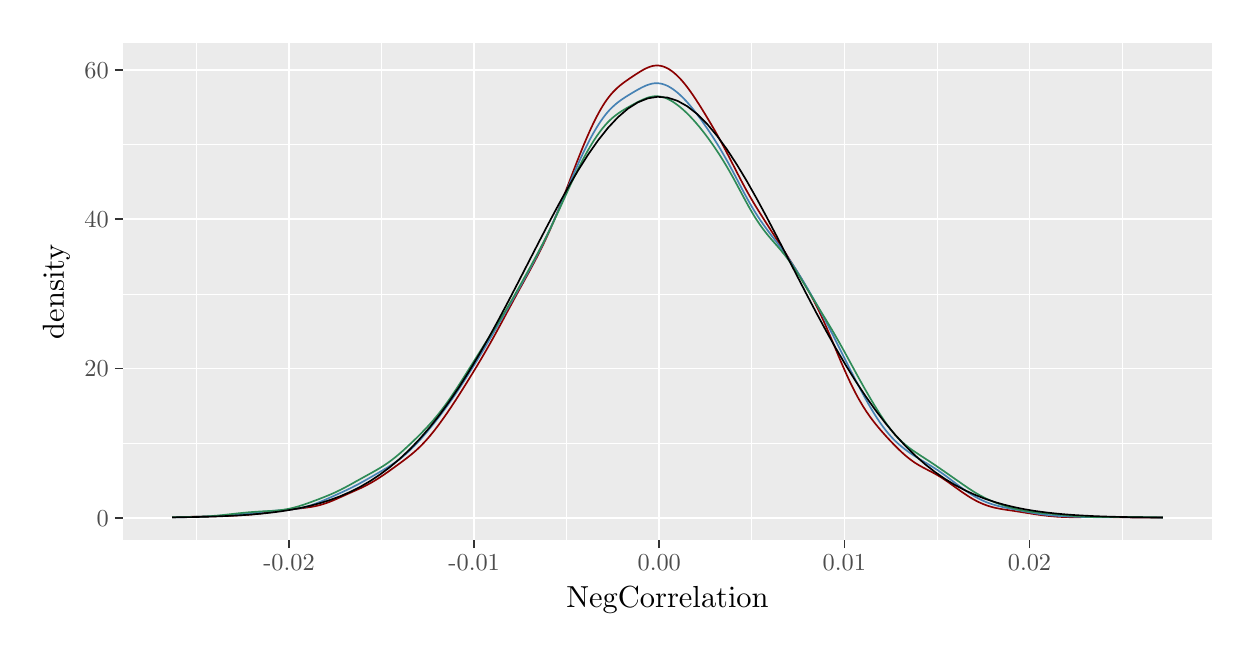
\begin{tikzpicture}[x=1pt,y=1pt]
\definecolor{fillColor}{RGB}{255,255,255}
\path[use as bounding box,fill=fillColor,fill opacity=0.00] (0,0) rectangle (433.62,216.81);
\begin{scope}
\path[clip] (  0.00,  0.00) rectangle (433.62,216.81);
\definecolor{drawColor}{RGB}{255,255,255}
\definecolor{fillColor}{RGB}{255,255,255}

\path[draw=drawColor,line width= 0.6pt,line join=round,line cap=round,fill=fillColor] (  0.00,  0.00) rectangle (433.62,216.81);
\end{scope}
\begin{scope}
\path[clip] ( 34.27, 31.53) rectangle (428.12,211.31);
\definecolor{fillColor}{gray}{0.92}

\path[fill=fillColor] ( 34.27, 31.53) rectangle (428.12,211.31);
\definecolor{drawColor}{RGB}{255,255,255}

\path[draw=drawColor,line width= 0.3pt,line join=round] ( 34.27, 66.67) --
	(428.12, 66.67);

\path[draw=drawColor,line width= 0.3pt,line join=round] ( 34.27,120.60) --
	(428.12,120.60);

\path[draw=drawColor,line width= 0.3pt,line join=round] ( 34.27,174.54) --
	(428.12,174.54);

\path[draw=drawColor,line width= 0.3pt,line join=round] ( 61.01, 31.53) --
	( 61.01,211.31);

\path[draw=drawColor,line width= 0.3pt,line join=round] (127.90, 31.53) --
	(127.90,211.31);

\path[draw=drawColor,line width= 0.3pt,line join=round] (194.78, 31.53) --
	(194.78,211.31);

\path[draw=drawColor,line width= 0.3pt,line join=round] (261.67, 31.53) --
	(261.67,211.31);

\path[draw=drawColor,line width= 0.3pt,line join=round] (328.56, 31.53) --
	(328.56,211.31);

\path[draw=drawColor,line width= 0.3pt,line join=round] (395.45, 31.53) --
	(395.45,211.31);

\path[draw=drawColor,line width= 0.6pt,line join=round] ( 34.27, 39.70) --
	(428.12, 39.70);

\path[draw=drawColor,line width= 0.6pt,line join=round] ( 34.27, 93.64) --
	(428.12, 93.64);

\path[draw=drawColor,line width= 0.6pt,line join=round] ( 34.27,147.57) --
	(428.12,147.57);

\path[draw=drawColor,line width= 0.6pt,line join=round] ( 34.27,201.50) --
	(428.12,201.50);

\path[draw=drawColor,line width= 0.6pt,line join=round] ( 94.45, 31.53) --
	( 94.45,211.31);

\path[draw=drawColor,line width= 0.6pt,line join=round] (161.34, 31.53) --
	(161.34,211.31);

\path[draw=drawColor,line width= 0.6pt,line join=round] (228.23, 31.53) --
	(228.23,211.31);

\path[draw=drawColor,line width= 0.6pt,line join=round] (295.12, 31.53) --
	(295.12,211.31);

\path[draw=drawColor,line width= 0.6pt,line join=round] (362.01, 31.53) --
	(362.01,211.31);
\definecolor{drawColor}{RGB}{139,0,0}

\path[draw=drawColor,line width= 0.6pt,line join=round] ( 52.17, 39.90) --
	( 52.87, 39.92) --
	( 53.57, 39.93) --
	( 54.27, 39.95) --
	( 54.97, 39.97) --
	( 55.67, 39.98) --
	( 56.37, 40.00) --
	( 57.07, 40.01) --
	( 57.78, 40.03) --
	( 58.48, 40.04) --
	( 59.18, 40.06) --
	( 59.88, 40.07) --
	( 60.58, 40.09) --
	( 61.28, 40.11) --
	( 61.98, 40.12) --
	( 62.68, 40.14) --
	( 63.38, 40.15) --
	( 64.08, 40.17) --
	( 64.78, 40.19) --
	( 65.48, 40.20) --
	( 66.18, 40.22) --
	( 66.88, 40.24) --
	( 67.59, 40.26) --
	( 68.29, 40.28) --
	( 68.99, 40.31) --
	( 69.69, 40.33) --
	( 70.39, 40.35) --
	( 71.09, 40.38) --
	( 71.79, 40.40) --
	( 72.49, 40.43) --
	( 73.19, 40.46) --
	( 73.89, 40.49) --
	( 74.59, 40.52) --
	( 75.29, 40.55) --
	( 75.99, 40.58) --
	( 76.69, 40.62) --
	( 77.39, 40.66) --
	( 78.10, 40.70) --
	( 78.80, 40.75) --
	( 79.50, 40.80) --
	( 80.20, 40.85) --
	( 80.90, 40.91) --
	( 81.60, 40.98) --
	( 82.30, 41.05) --
	( 83.00, 41.12) --
	( 83.70, 41.20) --
	( 84.40, 41.29) --
	( 85.10, 41.38) --
	( 85.80, 41.47) --
	( 86.50, 41.57) --
	( 87.20, 41.67) --
	( 87.90, 41.77) --
	( 88.61, 41.87) --
	( 89.31, 41.97) --
	( 90.01, 42.07) --
	( 90.71, 42.17) --
	( 91.41, 42.27) --
	( 92.11, 42.37) --
	( 92.81, 42.46) --
	( 93.51, 42.55) --
	( 94.21, 42.64) --
	( 94.91, 42.72) --
	( 95.61, 42.80) --
	( 96.31, 42.88) --
	( 97.01, 42.96) --
	( 97.71, 43.03) --
	( 98.42, 43.11) --
	( 99.12, 43.19) --
	( 99.82, 43.27) --
	(100.52, 43.35) --
	(101.22, 43.45) --
	(101.92, 43.55) --
	(102.62, 43.66) --
	(103.32, 43.79) --
	(104.02, 43.93) --
	(104.72, 44.09) --
	(105.42, 44.26) --
	(106.12, 44.45) --
	(106.82, 44.67) --
	(107.52, 44.89) --
	(108.22, 45.14) --
	(108.93, 45.41) --
	(109.63, 45.68) --
	(110.33, 45.97) --
	(111.03, 46.27) --
	(111.73, 46.57) --
	(112.43, 46.89) --
	(113.13, 47.20) --
	(113.83, 47.51) --
	(114.53, 47.83) --
	(115.23, 48.14) --
	(115.93, 48.45) --
	(116.63, 48.77) --
	(117.33, 49.08) --
	(118.03, 49.39) --
	(118.73, 49.70) --
	(119.44, 50.02) --
	(120.14, 50.34) --
	(120.84, 50.67) --
	(121.54, 51.01) --
	(122.24, 51.36) --
	(122.94, 51.73) --
	(123.64, 52.11) --
	(124.34, 52.50) --
	(125.04, 52.91) --
	(125.74, 53.33) --
	(126.44, 53.77) --
	(127.14, 54.22) --
	(127.84, 54.69) --
	(128.54, 55.16) --
	(129.24, 55.64) --
	(129.95, 56.13) --
	(130.65, 56.63) --
	(131.35, 57.13) --
	(132.05, 57.63) --
	(132.75, 58.14) --
	(133.45, 58.65) --
	(134.15, 59.16) --
	(134.85, 59.67) --
	(135.55, 60.19) --
	(136.25, 60.72) --
	(136.95, 61.25) --
	(137.65, 61.80) --
	(138.35, 62.36) --
	(139.05, 62.94) --
	(139.76, 63.54) --
	(140.46, 64.16) --
	(141.16, 64.81) --
	(141.86, 65.49) --
	(142.56, 66.19) --
	(143.26, 66.92) --
	(143.96, 67.68) --
	(144.66, 68.47) --
	(145.36, 69.29) --
	(146.06, 70.14) --
	(146.76, 71.01) --
	(147.46, 71.91) --
	(148.16, 72.83) --
	(148.86, 73.77) --
	(149.56, 74.74) --
	(150.27, 75.72) --
	(150.97, 76.71) --
	(151.67, 77.73) --
	(152.37, 78.76) --
	(153.07, 79.80) --
	(153.77, 80.86) --
	(154.47, 81.93) --
	(155.17, 83.01) --
	(155.87, 84.10) --
	(156.57, 85.21) --
	(157.27, 86.32) --
	(157.97, 87.44) --
	(158.67, 88.56) --
	(159.37, 89.70) --
	(160.07, 90.84) --
	(160.78, 91.98) --
	(161.48, 93.14) --
	(162.18, 94.29) --
	(162.88, 95.46) --
	(163.58, 96.63) --
	(164.28, 97.82) --
	(164.98, 99.02) --
	(165.68,100.22) --
	(166.38,101.45) --
	(167.08,102.68) --
	(167.78,103.93) --
	(168.48,105.19) --
	(169.18,106.46) --
	(169.88,107.75) --
	(170.59,109.05) --
	(171.29,110.35) --
	(171.99,111.66) --
	(172.69,112.97) --
	(173.39,114.28) --
	(174.09,115.58) --
	(174.79,116.88) --
	(175.49,118.18) --
	(176.19,119.47) --
	(176.89,120.76) --
	(177.59,122.04) --
	(178.29,123.31) --
	(178.99,124.58) --
	(179.69,125.86) --
	(180.39,127.13) --
	(181.10,128.42) --
	(181.80,129.71) --
	(182.50,131.02) --
	(183.20,132.34) --
	(183.90,133.68) --
	(184.60,135.05) --
	(185.30,136.44) --
	(186.00,137.86) --
	(186.70,139.31) --
	(187.40,140.80) --
	(188.10,142.33) --
	(188.80,143.90) --
	(189.50,145.51) --
	(190.20,147.15) --
	(190.90,148.83) --
	(191.61,150.55) --
	(192.31,152.30) --
	(193.01,154.08) --
	(193.71,155.89) --
	(194.41,157.71) --
	(195.11,159.54) --
	(195.81,161.38) --
	(196.51,163.22) --
	(197.21,165.05) --
	(197.91,166.86) --
	(198.61,168.66) --
	(199.31,170.44) --
	(200.01,172.18) --
	(200.71,173.90) --
	(201.42,175.58) --
	(202.12,177.22) --
	(202.82,178.82) --
	(203.52,180.37) --
	(204.22,181.86) --
	(204.92,183.30) --
	(205.62,184.67) --
	(206.32,185.99) --
	(207.02,187.24) --
	(207.72,188.42) --
	(208.42,189.53) --
	(209.12,190.56) --
	(209.82,191.51) --
	(210.52,192.39) --
	(211.22,193.21) --
	(211.93,193.96) --
	(212.63,194.66) --
	(213.33,195.30) --
	(214.03,195.90) --
	(214.73,196.46) --
	(215.43,196.98) --
	(216.13,197.49) --
	(216.83,197.98) --
	(217.53,198.46) --
	(218.23,198.93) --
	(218.93,199.40) --
	(219.63,199.86) --
	(220.33,200.31) --
	(221.03,200.75) --
	(221.73,201.18) --
	(222.44,201.58) --
	(223.14,201.95) --
	(223.84,202.28) --
	(224.54,202.57) --
	(225.24,202.81) --
	(225.94,202.99) --
	(226.64,203.10) --
	(227.34,203.14) --
	(228.04,203.11) --
	(228.74,203.01) --
	(229.44,202.84) --
	(230.14,202.60) --
	(230.84,202.30) --
	(231.54,201.92) --
	(232.24,201.47) --
	(232.95,200.97) --
	(233.65,200.41) --
	(234.35,199.79) --
	(235.05,199.12) --
	(235.75,198.40) --
	(236.45,197.63) --
	(237.15,196.81) --
	(237.85,195.94) --
	(238.55,195.02) --
	(239.25,194.07) --
	(239.95,193.08) --
	(240.65,192.05) --
	(241.35,191.00) --
	(242.05,189.92) --
	(242.76,188.82) --
	(243.46,187.71) --
	(244.16,186.57) --
	(244.86,185.43) --
	(245.56,184.27) --
	(246.26,183.10) --
	(246.96,181.92) --
	(247.66,180.72) --
	(248.36,179.51) --
	(249.06,178.27) --
	(249.76,177.02) --
	(250.46,175.74) --
	(251.16,174.44) --
	(251.86,173.13) --
	(252.56,171.79) --
	(253.27,170.44) --
	(253.97,169.07) --
	(254.67,167.70) --
	(255.37,166.33) --
	(256.07,164.96) --
	(256.77,163.60) --
	(257.47,162.25) --
	(258.17,160.92) --
	(258.87,159.61) --
	(259.57,158.32) --
	(260.27,157.07) --
	(260.97,155.84) --
	(261.67,154.63) --
	(262.37,153.44) --
	(263.07,152.28) --
	(263.78,151.14) --
	(264.48,150.01) --
	(265.18,148.89) --
	(265.88,147.79) --
	(266.58,146.69) --
	(267.28,145.60) --
	(267.98,144.51) --
	(268.68,143.42) --
	(269.38,142.33) --
	(270.08,141.23) --
	(270.78,140.14) --
	(271.48,139.04) --
	(272.18,137.94) --
	(272.88,136.83) --
	(273.59,135.73) --
	(274.29,134.62) --
	(274.99,133.51) --
	(275.69,132.39) --
	(276.39,131.28) --
	(277.09,130.15) --
	(277.79,129.03) --
	(278.49,127.89) --
	(279.19,126.74) --
	(279.89,125.58) --
	(280.59,124.40) --
	(281.29,123.20) --
	(281.99,121.98) --
	(282.69,120.72) --
	(283.39,119.42) --
	(284.10,118.09) --
	(284.80,116.72) --
	(285.50,115.31) --
	(286.20,113.86) --
	(286.90,112.37) --
	(287.60,110.84) --
	(288.30,109.26) --
	(289.00,107.66) --
	(289.70,106.03) --
	(290.40,104.38) --
	(291.10,102.71) --
	(291.80,101.04) --
	(292.50, 99.36) --
	(293.20, 97.69) --
	(293.90, 96.04) --
	(294.61, 94.42) --
	(295.31, 92.82) --
	(296.01, 91.25) --
	(296.71, 89.73) --
	(297.41, 88.24) --
	(298.11, 86.81) --
	(298.81, 85.42) --
	(299.51, 84.09) --
	(300.21, 82.81) --
	(300.91, 81.59) --
	(301.61, 80.41) --
	(302.31, 79.28) --
	(303.01, 78.20) --
	(303.71, 77.17) --
	(304.41, 76.18) --
	(305.12, 75.23) --
	(305.82, 74.31) --
	(306.52, 73.43) --
	(307.22, 72.58) --
	(307.92, 71.74) --
	(308.62, 70.93) --
	(309.32, 70.14) --
	(310.02, 69.36) --
	(310.72, 68.59) --
	(311.42, 67.84) --
	(312.12, 67.10) --
	(312.82, 66.37) --
	(313.52, 65.65) --
	(314.22, 64.95) --
	(314.93, 64.26) --
	(315.63, 63.60) --
	(316.33, 62.95) --
	(317.03, 62.33) --
	(317.73, 61.74) --
	(318.43, 61.18) --
	(319.13, 60.64) --
	(319.83, 60.13) --
	(320.53, 59.65) --
	(321.23, 59.20) --
	(321.93, 58.78) --
	(322.63, 58.37) --
	(323.33, 57.99) --
	(324.03, 57.61) --
	(324.73, 57.25) --
	(325.44, 56.89) --
	(326.14, 56.53) --
	(326.84, 56.16) --
	(327.54, 55.78) --
	(328.24, 55.39) --
	(328.94, 54.99) --
	(329.64, 54.57) --
	(330.34, 54.13) --
	(331.04, 53.67) --
	(331.74, 53.21) --
	(332.44, 52.72) --
	(333.14, 52.23) --
	(333.84, 51.72) --
	(334.54, 51.22) --
	(335.24, 50.71) --
	(335.95, 50.20) --
	(336.65, 49.70) --
	(337.35, 49.20) --
	(338.05, 48.71) --
	(338.75, 48.24) --
	(339.45, 47.78) --
	(340.15, 47.33) --
	(340.85, 46.90) --
	(341.55, 46.49) --
	(342.25, 46.10) --
	(342.95, 45.73) --
	(343.65, 45.38) --
	(344.35, 45.06) --
	(345.05, 44.76) --
	(345.76, 44.48) --
	(346.46, 44.22) --
	(347.16, 43.98) --
	(347.86, 43.77) --
	(348.56, 43.57) --
	(349.26, 43.39) --
	(349.96, 43.23) --
	(350.66, 43.09) --
	(351.36, 42.95) --
	(352.06, 42.83) --
	(352.76, 42.72) --
	(353.46, 42.61) --
	(354.16, 42.50) --
	(354.86, 42.40) --
	(355.56, 42.30) --
	(356.27, 42.20) --
	(356.97, 42.09) --
	(357.67, 41.99) --
	(358.37, 41.88) --
	(359.07, 41.77) --
	(359.77, 41.66) --
	(360.47, 41.55) --
	(361.17, 41.44) --
	(361.87, 41.33) --
	(362.57, 41.22) --
	(363.27, 41.11) --
	(363.97, 41.00) --
	(364.67, 40.90) --
	(365.37, 40.80) --
	(366.07, 40.70) --
	(366.78, 40.61) --
	(367.48, 40.53) --
	(368.18, 40.45) --
	(368.88, 40.37) --
	(369.58, 40.30) --
	(370.28, 40.23) --
	(370.98, 40.18) --
	(371.68, 40.12) --
	(372.38, 40.08) --
	(373.08, 40.04) --
	(373.78, 40.00) --
	(374.48, 39.98) --
	(375.18, 39.95) --
	(375.88, 39.94) --
	(376.58, 39.92) --
	(377.29, 39.92) --
	(377.99, 39.91) --
	(378.69, 39.92) --
	(379.39, 39.92) --
	(380.09, 39.92) --
	(380.79, 39.93) --
	(381.49, 39.94) --
	(382.19, 39.95) --
	(382.89, 39.95) --
	(383.59, 39.96) --
	(384.29, 39.97) --
	(384.99, 39.97) --
	(385.69, 39.97) --
	(386.39, 39.97) --
	(387.10, 39.97) --
	(387.80, 39.97) --
	(388.50, 39.97) --
	(389.20, 39.96) --
	(389.90, 39.95) --
	(390.60, 39.94) --
	(391.30, 39.94) --
	(392.00, 39.93) --
	(392.70, 39.92) --
	(393.40, 39.91) --
	(394.10, 39.90) --
	(394.80, 39.89) --
	(395.50, 39.87) --
	(396.20, 39.86) --
	(396.90, 39.86) --
	(397.61, 39.85) --
	(398.31, 39.84) --
	(399.01, 39.83) --
	(399.71, 39.83) --
	(400.41, 39.82) --
	(401.11, 39.82) --
	(401.81, 39.81) --
	(402.51, 39.81) --
	(403.21, 39.81) --
	(403.91, 39.81) --
	(404.61, 39.81) --
	(405.31, 39.81) --
	(406.01, 39.82) --
	(406.71, 39.82) --
	(407.41, 39.82) --
	(408.12, 39.82) --
	(408.82, 39.82) --
	(409.52, 39.82) --
	(410.22, 39.82);
\definecolor{drawColor}{RGB}{70,130,180}

\path[draw=drawColor,line width= 0.6pt,line join=round] ( 52.17, 39.85) --
	( 52.87, 39.86) --
	( 53.57, 39.87) --
	( 54.27, 39.88) --
	( 54.97, 39.90) --
	( 55.67, 39.91) --
	( 56.37, 39.92) --
	( 57.07, 39.94) --
	( 57.78, 39.95) --
	( 58.48, 39.97) --
	( 59.18, 39.99) --
	( 59.88, 40.02) --
	( 60.58, 40.04) --
	( 61.28, 40.07) --
	( 61.98, 40.09) --
	( 62.68, 40.12) --
	( 63.38, 40.15) --
	( 64.08, 40.18) --
	( 64.78, 40.21) --
	( 65.48, 40.25) --
	( 66.18, 40.28) --
	( 66.88, 40.31) --
	( 67.59, 40.35) --
	( 68.29, 40.38) --
	( 68.99, 40.42) --
	( 69.69, 40.46) --
	( 70.39, 40.50) --
	( 71.09, 40.54) --
	( 71.79, 40.58) --
	( 72.49, 40.63) --
	( 73.19, 40.67) --
	( 73.89, 40.73) --
	( 74.59, 40.78) --
	( 75.29, 40.84) --
	( 75.99, 40.90) --
	( 76.69, 40.97) --
	( 77.39, 41.04) --
	( 78.10, 41.11) --
	( 78.80, 41.18) --
	( 79.50, 41.26) --
	( 80.20, 41.34) --
	( 80.90, 41.42) --
	( 81.60, 41.50) --
	( 82.30, 41.58) --
	( 83.00, 41.66) --
	( 83.70, 41.74) --
	( 84.40, 41.81) --
	( 85.10, 41.89) --
	( 85.80, 41.96) --
	( 86.50, 42.03) --
	( 87.20, 42.09) --
	( 87.90, 42.15) --
	( 88.61, 42.21) --
	( 89.31, 42.26) --
	( 90.01, 42.31) --
	( 90.71, 42.36) --
	( 91.41, 42.41) --
	( 92.11, 42.46) --
	( 92.81, 42.51) --
	( 93.51, 42.57) --
	( 94.21, 42.63) --
	( 94.91, 42.70) --
	( 95.61, 42.77) --
	( 96.31, 42.86) --
	( 97.01, 42.96) --
	( 97.71, 43.08) --
	( 98.42, 43.21) --
	( 99.12, 43.35) --
	( 99.82, 43.51) --
	(100.52, 43.69) --
	(101.22, 43.89) --
	(101.92, 44.10) --
	(102.62, 44.33) --
	(103.32, 44.57) --
	(104.02, 44.82) --
	(104.72, 45.09) --
	(105.42, 45.37) --
	(106.12, 45.65) --
	(106.82, 45.95) --
	(107.52, 46.25) --
	(108.22, 46.55) --
	(108.93, 46.86) --
	(109.63, 47.17) --
	(110.33, 47.48) --
	(111.03, 47.80) --
	(111.73, 48.11) --
	(112.43, 48.43) --
	(113.13, 48.75) --
	(113.83, 49.07) --
	(114.53, 49.39) --
	(115.23, 49.72) --
	(115.93, 50.05) --
	(116.63, 50.39) --
	(117.33, 50.74) --
	(118.03, 51.10) --
	(118.73, 51.46) --
	(119.44, 51.83) --
	(120.14, 52.21) --
	(120.84, 52.60) --
	(121.54, 52.99) --
	(122.24, 53.38) --
	(122.94, 53.78) --
	(123.64, 54.18) --
	(124.34, 54.58) --
	(125.04, 54.98) --
	(125.74, 55.38) --
	(126.44, 55.79) --
	(127.14, 56.19) --
	(127.84, 56.60) --
	(128.54, 57.02) --
	(129.24, 57.44) --
	(129.95, 57.86) --
	(130.65, 58.30) --
	(131.35, 58.75) --
	(132.05, 59.21) --
	(132.75, 59.69) --
	(133.45, 60.18) --
	(134.15, 60.70) --
	(134.85, 61.25) --
	(135.55, 61.81) --
	(136.25, 62.40) --
	(136.95, 63.01) --
	(137.65, 63.64) --
	(138.35, 64.30) --
	(139.05, 64.99) --
	(139.76, 65.69) --
	(140.46, 66.42) --
	(141.16, 67.17) --
	(141.86, 67.94) --
	(142.56, 68.73) --
	(143.26, 69.53) --
	(143.96, 70.35) --
	(144.66, 71.19) --
	(145.36, 72.04) --
	(146.06, 72.90) --
	(146.76, 73.77) --
	(147.46, 74.66) --
	(148.16, 75.56) --
	(148.86, 76.47) --
	(149.56, 77.39) --
	(150.27, 78.33) --
	(150.97, 79.28) --
	(151.67, 80.24) --
	(152.37, 81.22) --
	(153.07, 82.21) --
	(153.77, 83.22) --
	(154.47, 84.24) --
	(155.17, 85.28) --
	(155.87, 86.33) --
	(156.57, 87.39) --
	(157.27, 88.47) --
	(157.97, 89.55) --
	(158.67, 90.65) --
	(159.37, 91.75) --
	(160.07, 92.87) --
	(160.78, 93.99) --
	(161.48, 95.12) --
	(162.18, 96.25) --
	(162.88, 97.40) --
	(163.58, 98.55) --
	(164.28, 99.71) --
	(164.98,100.88) --
	(165.68,102.05) --
	(166.38,103.23) --
	(167.08,104.42) --
	(167.78,105.61) --
	(168.48,106.81) --
	(169.18,108.01) --
	(169.88,109.21) --
	(170.59,110.42) --
	(171.29,111.63) --
	(171.99,112.84) --
	(172.69,114.05) --
	(173.39,115.26) --
	(174.09,116.48) --
	(174.79,117.69) --
	(175.49,118.91) --
	(176.19,120.14) --
	(176.89,121.37) --
	(177.59,122.61) --
	(178.29,123.86) --
	(178.99,125.11) --
	(179.69,126.37) --
	(180.39,127.64) --
	(181.10,128.93) --
	(181.80,130.22) --
	(182.50,131.53) --
	(183.20,132.85) --
	(183.90,134.19) --
	(184.60,135.55) --
	(185.30,136.93) --
	(186.00,138.33) --
	(186.70,139.75) --
	(187.40,141.20) --
	(188.10,142.68) --
	(188.80,144.19) --
	(189.50,145.73) --
	(190.20,147.29) --
	(190.90,148.88) --
	(191.61,150.49) --
	(192.31,152.13) --
	(193.01,153.78) --
	(193.71,155.44) --
	(194.41,157.10) --
	(195.11,158.77) --
	(195.81,160.43) --
	(196.51,162.09) --
	(197.21,163.72) --
	(197.91,165.34) --
	(198.61,166.93) --
	(199.31,168.49) --
	(200.01,170.02) --
	(200.71,171.51) --
	(201.42,172.97) --
	(202.12,174.38) --
	(202.82,175.75) --
	(203.52,177.08) --
	(204.22,178.36) --
	(204.92,179.58) --
	(205.62,180.75) --
	(206.32,181.87) --
	(207.02,182.93) --
	(207.72,183.93) --
	(208.42,184.87) --
	(209.12,185.76) --
	(209.82,186.58) --
	(210.52,187.34) --
	(211.22,188.04) --
	(211.93,188.69) --
	(212.63,189.30) --
	(213.33,189.86) --
	(214.03,190.39) --
	(214.73,190.89) --
	(215.43,191.36) --
	(216.13,191.81) --
	(216.83,192.25) --
	(217.53,192.68) --
	(218.23,193.10) --
	(218.93,193.52) --
	(219.63,193.93) --
	(220.33,194.33) --
	(221.03,194.72) --
	(221.73,195.09) --
	(222.44,195.44) --
	(223.14,195.76) --
	(223.84,196.05) --
	(224.54,196.29) --
	(225.24,196.49) --
	(225.94,196.64) --
	(226.64,196.72) --
	(227.34,196.74) --
	(228.04,196.70) --
	(228.74,196.60) --
	(229.44,196.44) --
	(230.14,196.21) --
	(230.84,195.93) --
	(231.54,195.59) --
	(232.24,195.18) --
	(232.95,194.73) --
	(233.65,194.24) --
	(234.35,193.69) --
	(235.05,193.11) --
	(235.75,192.49) --
	(236.45,191.82) --
	(237.15,191.12) --
	(237.85,190.38) --
	(238.55,189.61) --
	(239.25,188.80) --
	(239.95,187.96) --
	(240.65,187.09) --
	(241.35,186.20) --
	(242.05,185.28) --
	(242.76,184.33) --
	(243.46,183.37) --
	(244.16,182.38) --
	(244.86,181.37) --
	(245.56,180.35) --
	(246.26,179.31) --
	(246.96,178.25) --
	(247.66,177.18) --
	(248.36,176.08) --
	(249.06,174.96) --
	(249.76,173.82) --
	(250.46,172.65) --
	(251.16,171.45) --
	(251.86,170.23) --
	(252.56,168.99) --
	(253.27,167.72) --
	(253.97,166.42) --
	(254.67,165.11) --
	(255.37,163.78) --
	(256.07,162.45) --
	(256.77,161.11) --
	(257.47,159.77) --
	(258.17,158.44) --
	(258.87,157.12) --
	(259.57,155.83) --
	(260.27,154.56) --
	(260.97,153.32) --
	(261.67,152.11) --
	(262.37,150.94) --
	(263.07,149.80) --
	(263.78,148.70) --
	(264.48,147.64) --
	(265.18,146.61) --
	(265.88,145.61) --
	(266.58,144.64) --
	(267.28,143.69) --
	(267.98,142.76) --
	(268.68,141.84) --
	(269.38,140.93) --
	(270.08,140.02) --
	(270.78,139.10) --
	(271.48,138.18) --
	(272.18,137.25) --
	(272.88,136.30) --
	(273.59,135.34) --
	(274.29,134.35) --
	(274.99,133.35) --
	(275.69,132.32) --
	(276.39,131.28) --
	(277.09,130.21) --
	(277.79,129.13) --
	(278.49,128.02) --
	(279.19,126.90) --
	(279.89,125.76) --
	(280.59,124.60) --
	(281.29,123.43) --
	(281.99,122.24) --
	(282.69,121.03) --
	(283.39,119.81) --
	(284.10,118.58) --
	(284.80,117.33) --
	(285.50,116.06) --
	(286.20,114.78) --
	(286.90,113.49) --
	(287.60,112.18) --
	(288.30,110.86) --
	(289.00,109.52) --
	(289.70,108.17) --
	(290.40,106.81) --
	(291.10,105.44) --
	(291.80,104.06) --
	(292.50,102.67) --
	(293.20,101.28) --
	(293.90, 99.88) --
	(294.61, 98.48) --
	(295.31, 97.07) --
	(296.01, 95.68) --
	(296.71, 94.28) --
	(297.41, 92.89) --
	(298.11, 91.51) --
	(298.81, 90.14) --
	(299.51, 88.79) --
	(300.21, 87.44) --
	(300.91, 86.11) --
	(301.61, 84.80) --
	(302.31, 83.51) --
	(303.01, 82.25) --
	(303.71, 81.00) --
	(304.41, 79.79) --
	(305.12, 78.61) --
	(305.82, 77.45) --
	(306.52, 76.34) --
	(307.22, 75.26) --
	(307.92, 74.22) --
	(308.62, 73.23) --
	(309.32, 72.28) --
	(310.02, 71.37) --
	(310.72, 70.50) --
	(311.42, 69.68) --
	(312.12, 68.89) --
	(312.82, 68.15) --
	(313.52, 67.45) --
	(314.22, 66.79) --
	(314.93, 66.15) --
	(315.63, 65.55) --
	(316.33, 64.98) --
	(317.03, 64.43) --
	(317.73, 63.91) --
	(318.43, 63.41) --
	(319.13, 62.92) --
	(319.83, 62.46) --
	(320.53, 62.00) --
	(321.23, 61.56) --
	(321.93, 61.13) --
	(322.63, 60.71) --
	(323.33, 60.29) --
	(324.03, 59.87) --
	(324.73, 59.46) --
	(325.44, 59.04) --
	(326.14, 58.61) --
	(326.84, 58.18) --
	(327.54, 57.74) --
	(328.24, 57.29) --
	(328.94, 56.83) --
	(329.64, 56.35) --
	(330.34, 55.86) --
	(331.04, 55.36) --
	(331.74, 54.85) --
	(332.44, 54.33) --
	(333.14, 53.81) --
	(333.84, 53.28) --
	(334.54, 52.74) --
	(335.24, 52.21) --
	(335.95, 51.68) --
	(336.65, 51.15) --
	(337.35, 50.63) --
	(338.05, 50.13) --
	(338.75, 49.63) --
	(339.45, 49.15) --
	(340.15, 48.68) --
	(340.85, 48.24) --
	(341.55, 47.81) --
	(342.25, 47.40) --
	(342.95, 47.01) --
	(343.65, 46.63) --
	(344.35, 46.28) --
	(345.05, 45.95) --
	(345.76, 45.64) --
	(346.46, 45.35) --
	(347.16, 45.08) --
	(347.86, 44.83) --
	(348.56, 44.60) --
	(349.26, 44.38) --
	(349.96, 44.18) --
	(350.66, 43.99) --
	(351.36, 43.82) --
	(352.06, 43.65) --
	(352.76, 43.49) --
	(353.46, 43.34) --
	(354.16, 43.20) --
	(354.86, 43.06) --
	(355.56, 42.92) --
	(356.27, 42.78) --
	(356.97, 42.65) --
	(357.67, 42.51) --
	(358.37, 42.38) --
	(359.07, 42.24) --
	(359.77, 42.11) --
	(360.47, 41.97) --
	(361.17, 41.84) --
	(361.87, 41.71) --
	(362.57, 41.58) --
	(363.27, 41.46) --
	(363.97, 41.34) --
	(364.67, 41.22) --
	(365.37, 41.11) --
	(366.07, 41.01) --
	(366.78, 40.92) --
	(367.48, 40.83) --
	(368.18, 40.75) --
	(368.88, 40.67) --
	(369.58, 40.60) --
	(370.28, 40.54) --
	(370.98, 40.48) --
	(371.68, 40.43) --
	(372.38, 40.38) --
	(373.08, 40.34) --
	(373.78, 40.30) --
	(374.48, 40.26) --
	(375.18, 40.22) --
	(375.88, 40.19) --
	(376.58, 40.16) --
	(377.29, 40.13) --
	(377.99, 40.11) --
	(378.69, 40.08) --
	(379.39, 40.06) --
	(380.09, 40.04) --
	(380.79, 40.01) --
	(381.49, 40.00) --
	(382.19, 39.98) --
	(382.89, 39.96) --
	(383.59, 39.95) --
	(384.29, 39.94) --
	(384.99, 39.93) --
	(385.69, 39.92) --
	(386.39, 39.92) --
	(387.10, 39.92) --
	(387.80, 39.92) --
	(388.50, 39.92) --
	(389.20, 39.92) --
	(389.90, 39.92) --
	(390.60, 39.92) --
	(391.30, 39.92) --
	(392.00, 39.93) --
	(392.70, 39.93) --
	(393.40, 39.93) --
	(394.10, 39.93) --
	(394.80, 39.93) --
	(395.50, 39.93) --
	(396.20, 39.92) --
	(396.90, 39.92) --
	(397.61, 39.92) --
	(398.31, 39.91) --
	(399.01, 39.91) --
	(399.71, 39.90) --
	(400.41, 39.90) --
	(401.11, 39.89) --
	(401.81, 39.89) --
	(402.51, 39.88) --
	(403.21, 39.87) --
	(403.91, 39.87) --
	(404.61, 39.86) --
	(405.31, 39.86) --
	(406.01, 39.86) --
	(406.71, 39.85) --
	(407.41, 39.85) --
	(408.12, 39.84) --
	(408.82, 39.83) --
	(409.52, 39.83) --
	(410.22, 39.82);
\definecolor{drawColor}{RGB}{46,139,87}

\path[draw=drawColor,line width= 0.6pt,line join=round] ( 52.17, 39.91) --
	( 52.87, 39.92) --
	( 53.57, 39.93) --
	( 54.27, 39.95) --
	( 54.97, 39.96) --
	( 55.67, 39.97) --
	( 56.37, 39.98) --
	( 57.07, 39.99) --
	( 57.78, 40.01) --
	( 58.48, 40.02) --
	( 59.18, 40.03) --
	( 59.88, 40.05) --
	( 60.58, 40.07) --
	( 61.28, 40.09) --
	( 61.98, 40.11) --
	( 62.68, 40.13) --
	( 63.38, 40.16) --
	( 64.08, 40.19) --
	( 64.78, 40.23) --
	( 65.48, 40.27) --
	( 66.18, 40.32) --
	( 66.88, 40.37) --
	( 67.59, 40.43) --
	( 68.29, 40.49) --
	( 68.99, 40.55) --
	( 69.69, 40.62) --
	( 70.39, 40.69) --
	( 71.09, 40.77) --
	( 71.79, 40.84) --
	( 72.49, 40.92) --
	( 73.19, 41.00) --
	( 73.89, 41.08) --
	( 74.59, 41.15) --
	( 75.29, 41.23) --
	( 75.99, 41.31) --
	( 76.69, 41.38) --
	( 77.39, 41.46) --
	( 78.10, 41.53) --
	( 78.80, 41.59) --
	( 79.50, 41.66) --
	( 80.20, 41.72) --
	( 80.90, 41.77) --
	( 81.60, 41.83) --
	( 82.30, 41.88) --
	( 83.00, 41.93) --
	( 83.70, 41.97) --
	( 84.40, 42.01) --
	( 85.10, 42.05) --
	( 85.80, 42.08) --
	( 86.50, 42.12) --
	( 87.20, 42.16) --
	( 87.90, 42.20) --
	( 88.61, 42.24) --
	( 89.31, 42.29) --
	( 90.01, 42.35) --
	( 90.71, 42.42) --
	( 91.41, 42.49) --
	( 92.11, 42.58) --
	( 92.81, 42.69) --
	( 93.51, 42.80) --
	( 94.21, 42.93) --
	( 94.91, 43.08) --
	( 95.61, 43.24) --
	( 96.31, 43.42) --
	( 97.01, 43.61) --
	( 97.71, 43.81) --
	( 98.42, 44.02) --
	( 99.12, 44.25) --
	( 99.82, 44.48) --
	(100.52, 44.72) --
	(101.22, 44.97) --
	(101.92, 45.22) --
	(102.62, 45.48) --
	(103.32, 45.74) --
	(104.02, 46.00) --
	(104.72, 46.26) --
	(105.42, 46.53) --
	(106.12, 46.80) --
	(106.82, 47.08) --
	(107.52, 47.36) --
	(108.22, 47.64) --
	(108.93, 47.93) --
	(109.63, 48.23) --
	(110.33, 48.54) --
	(111.03, 48.85) --
	(111.73, 49.18) --
	(112.43, 49.52) --
	(113.13, 49.86) --
	(113.83, 50.22) --
	(114.53, 50.59) --
	(115.23, 50.96) --
	(115.93, 51.34) --
	(116.63, 51.72) --
	(117.33, 52.11) --
	(118.03, 52.50) --
	(118.73, 52.90) --
	(119.44, 53.29) --
	(120.14, 53.68) --
	(120.84, 54.07) --
	(121.54, 54.45) --
	(122.24, 54.84) --
	(122.94, 55.23) --
	(123.64, 55.61) --
	(124.34, 56.00) --
	(125.04, 56.39) --
	(125.74, 56.79) --
	(126.44, 57.19) --
	(127.14, 57.61) --
	(127.84, 58.04) --
	(128.54, 58.48) --
	(129.24, 58.94) --
	(129.95, 59.42) --
	(130.65, 59.91) --
	(131.35, 60.43) --
	(132.05, 60.97) --
	(132.75, 61.52) --
	(133.45, 62.09) --
	(134.15, 62.68) --
	(134.85, 63.29) --
	(135.55, 63.90) --
	(136.25, 64.54) --
	(136.95, 65.18) --
	(137.65, 65.83) --
	(138.35, 66.49) --
	(139.05, 67.16) --
	(139.76, 67.83) --
	(140.46, 68.52) --
	(141.16, 69.21) --
	(141.86, 69.91) --
	(142.56, 70.62) --
	(143.26, 71.34) --
	(143.96, 72.08) --
	(144.66, 72.83) --
	(145.36, 73.60) --
	(146.06, 74.38) --
	(146.76, 75.19) --
	(147.46, 76.02) --
	(148.16, 76.88) --
	(148.86, 77.76) --
	(149.56, 78.66) --
	(150.27, 79.59) --
	(150.97, 80.54) --
	(151.67, 81.51) --
	(152.37, 82.51) --
	(153.07, 83.53) --
	(153.77, 84.56) --
	(154.47, 85.62) --
	(155.17, 86.69) --
	(155.87, 87.77) --
	(156.57, 88.86) --
	(157.27, 89.96) --
	(157.97, 91.07) --
	(158.67, 92.18) --
	(159.37, 93.30) --
	(160.07, 94.41) --
	(160.78, 95.53) --
	(161.48, 96.65) --
	(162.18, 97.77) --
	(162.88, 98.88) --
	(163.58, 99.99) --
	(164.28,101.10) --
	(164.98,102.21) --
	(165.68,103.31) --
	(166.38,104.42) --
	(167.08,105.52) --
	(167.78,106.63) --
	(168.48,107.74) --
	(169.18,108.86) --
	(169.88,109.99) --
	(170.59,111.12) --
	(171.29,112.26) --
	(171.99,113.42) --
	(172.69,114.58) --
	(173.39,115.77) --
	(174.09,116.96) --
	(174.79,118.16) --
	(175.49,119.38) --
	(176.19,120.61) --
	(176.89,121.85) --
	(177.59,123.09) --
	(178.29,124.35) --
	(178.99,125.61) --
	(179.69,126.87) --
	(180.39,128.14) --
	(181.10,129.41) --
	(181.80,130.69) --
	(182.50,131.97) --
	(183.20,133.26) --
	(183.90,134.56) --
	(184.60,135.87) --
	(185.30,137.19) --
	(186.00,138.53) --
	(186.70,139.89) --
	(187.40,141.27) --
	(188.10,142.68) --
	(188.80,144.11) --
	(189.50,145.56) --
	(190.20,147.04) --
	(190.90,148.54) --
	(191.61,150.06) --
	(192.31,151.59) --
	(193.01,153.13) --
	(193.71,154.68) --
	(194.41,156.23) --
	(195.11,157.77) --
	(195.81,159.30) --
	(196.51,160.81) --
	(197.21,162.30) --
	(197.91,163.77) --
	(198.61,165.21) --
	(199.31,166.62) --
	(200.01,167.99) --
	(200.71,169.32) --
	(201.42,170.62) --
	(202.12,171.89) --
	(202.82,173.11) --
	(203.52,174.30) --
	(204.22,175.44) --
	(204.92,176.54) --
	(205.62,177.58) --
	(206.32,178.58) --
	(207.02,179.53) --
	(207.72,180.43) --
	(208.42,181.28) --
	(209.12,182.07) --
	(209.82,182.82) --
	(210.52,183.50) --
	(211.22,184.13) --
	(211.93,184.72) --
	(212.63,185.27) --
	(213.33,185.78) --
	(214.03,186.26) --
	(214.73,186.72) --
	(215.43,187.15) --
	(216.13,187.56) --
	(216.83,187.97) --
	(217.53,188.36) --
	(218.23,188.75) --
	(218.93,189.13) --
	(219.63,189.51) --
	(220.33,189.88) --
	(221.03,190.23) --
	(221.73,190.57) --
	(222.44,190.89) --
	(223.14,191.18) --
	(223.84,191.44) --
	(224.54,191.66) --
	(225.24,191.83) --
	(225.94,191.96) --
	(226.64,192.03) --
	(227.34,192.04) --
	(228.04,191.99) --
	(228.74,191.89) --
	(229.44,191.73) --
	(230.14,191.51) --
	(230.84,191.24) --
	(231.54,190.92) --
	(232.24,190.55) --
	(232.95,190.14) --
	(233.65,189.68) --
	(234.35,189.19) --
	(235.05,188.67) --
	(235.75,188.11) --
	(236.45,187.52) --
	(237.15,186.90) --
	(237.85,186.25) --
	(238.55,185.56) --
	(239.25,184.86) --
	(239.95,184.12) --
	(240.65,183.36) --
	(241.35,182.57) --
	(242.05,181.75) --
	(242.76,180.91) --
	(243.46,180.04) --
	(244.16,179.15) --
	(244.86,178.24) --
	(245.56,177.30) --
	(246.26,176.35) --
	(246.96,175.37) --
	(247.66,174.38) --
	(248.36,173.36) --
	(249.06,172.31) --
	(249.76,171.25) --
	(250.46,170.15) --
	(251.16,169.04) --
	(251.86,167.89) --
	(252.56,166.72) --
	(253.27,165.51) --
	(253.97,164.28) --
	(254.67,163.03) --
	(255.37,161.76) --
	(256.07,160.47) --
	(256.77,159.16) --
	(257.47,157.85) --
	(258.17,156.54) --
	(258.87,155.23) --
	(259.57,153.94) --
	(260.27,152.67) --
	(260.97,151.42) --
	(261.67,150.21) --
	(262.37,149.03) --
	(263.07,147.90) --
	(263.78,146.82) --
	(264.48,145.78) --
	(265.18,144.79) --
	(265.88,143.84) --
	(266.58,142.93) --
	(267.28,142.05) --
	(267.98,141.21) --
	(268.68,140.39) --
	(269.38,139.59) --
	(270.08,138.79) --
	(270.78,137.99) --
	(271.48,137.18) --
	(272.18,136.35) --
	(272.88,135.50) --
	(273.59,134.63) --
	(274.29,133.72) --
	(274.99,132.77) --
	(275.69,131.79) --
	(276.39,130.78) --
	(277.09,129.74) --
	(277.79,128.67) --
	(278.49,127.58) --
	(279.19,126.46) --
	(279.89,125.32) --
	(280.59,124.18) --
	(281.29,123.02) --
	(281.99,121.87) --
	(282.69,120.71) --
	(283.39,119.55) --
	(284.10,118.40) --
	(284.80,117.25) --
	(285.50,116.10) --
	(286.20,114.96) --
	(286.90,113.81) --
	(287.60,112.67) --
	(288.30,111.52) --
	(289.00,110.36) --
	(289.70,109.20) --
	(290.40,108.02) --
	(291.10,106.83) --
	(291.80,105.62) --
	(292.50,104.40) --
	(293.20,103.17) --
	(293.90,101.92) --
	(294.61,100.66) --
	(295.31, 99.39) --
	(296.01, 98.11) --
	(296.71, 96.82) --
	(297.41, 95.53) --
	(298.11, 94.24) --
	(298.81, 92.96) --
	(299.51, 91.68) --
	(300.21, 90.40) --
	(300.91, 89.14) --
	(301.61, 87.89) --
	(302.31, 86.64) --
	(303.01, 85.42) --
	(303.71, 84.20) --
	(304.41, 83.00) --
	(305.12, 81.81) --
	(305.82, 80.64) --
	(306.52, 79.49) --
	(307.22, 78.37) --
	(307.92, 77.26) --
	(308.62, 76.18) --
	(309.32, 75.13) --
	(310.02, 74.12) --
	(310.72, 73.13) --
	(311.42, 72.19) --
	(312.12, 71.30) --
	(312.82, 70.44) --
	(313.52, 69.63) --
	(314.22, 68.86) --
	(314.93, 68.13) --
	(315.63, 67.44) --
	(316.33, 66.80) --
	(317.03, 66.20) --
	(317.73, 65.63) --
	(318.43, 65.08) --
	(319.13, 64.56) --
	(319.83, 64.06) --
	(320.53, 63.58) --
	(321.23, 63.11) --
	(321.93, 62.65) --
	(322.63, 62.19) --
	(323.33, 61.74) --
	(324.03, 61.28) --
	(324.73, 60.83) --
	(325.44, 60.37) --
	(326.14, 59.91) --
	(326.84, 59.44) --
	(327.54, 58.97) --
	(328.24, 58.50) --
	(328.94, 58.02) --
	(329.64, 57.54) --
	(330.34, 57.06) --
	(331.04, 56.58) --
	(331.74, 56.09) --
	(332.44, 55.60) --
	(333.14, 55.11) --
	(333.84, 54.62) --
	(334.54, 54.13) --
	(335.24, 53.64) --
	(335.95, 53.14) --
	(336.65, 52.65) --
	(337.35, 52.16) --
	(338.05, 51.68) --
	(338.75, 51.20) --
	(339.45, 50.72) --
	(340.15, 50.25) --
	(340.85, 49.80) --
	(341.55, 49.35) --
	(342.25, 48.91) --
	(342.95, 48.49) --
	(343.65, 48.09) --
	(344.35, 47.69) --
	(345.05, 47.32) --
	(345.76, 46.96) --
	(346.46, 46.61) --
	(347.16, 46.28) --
	(347.86, 45.97) --
	(348.56, 45.67) --
	(349.26, 45.38) --
	(349.96, 45.11) --
	(350.66, 44.84) --
	(351.36, 44.59) --
	(352.06, 44.35) --
	(352.76, 44.12) --
	(353.46, 43.90) --
	(354.16, 43.69) --
	(354.86, 43.48) --
	(355.56, 43.29) --
	(356.27, 43.11) --
	(356.97, 42.93) --
	(357.67, 42.77) --
	(358.37, 42.61) --
	(359.07, 42.47) --
	(359.77, 42.33) --
	(360.47, 42.21) --
	(361.17, 42.09) --
	(361.87, 41.98) --
	(362.57, 41.89) --
	(363.27, 41.79) --
	(363.97, 41.71) --
	(364.67, 41.63) --
	(365.37, 41.56) --
	(366.07, 41.49) --
	(366.78, 41.42) --
	(367.48, 41.35) --
	(368.18, 41.29) --
	(368.88, 41.22) --
	(369.58, 41.16) --
	(370.28, 41.10) --
	(370.98, 41.03) --
	(371.68, 40.97) --
	(372.38, 40.90) --
	(373.08, 40.83) --
	(373.78, 40.76) --
	(374.48, 40.70) --
	(375.18, 40.63) --
	(375.88, 40.56) --
	(376.58, 40.50) --
	(377.29, 40.44) --
	(377.99, 40.38) --
	(378.69, 40.32) --
	(379.39, 40.27) --
	(380.09, 40.22) --
	(380.79, 40.17) --
	(381.49, 40.13) --
	(382.19, 40.10) --
	(382.89, 40.06) --
	(383.59, 40.03) --
	(384.29, 40.01) --
	(384.99, 39.99) --
	(385.69, 39.97) --
	(386.39, 39.96) --
	(387.10, 39.95) --
	(387.80, 39.94) --
	(388.50, 39.94) --
	(389.20, 39.94) --
	(389.90, 39.94) --
	(390.60, 39.94) --
	(391.30, 39.94) --
	(392.00, 39.95) --
	(392.70, 39.95) --
	(393.40, 39.96) --
	(394.10, 39.97) --
	(394.80, 39.97) --
	(395.50, 39.98) --
	(396.20, 39.98) --
	(396.90, 39.99) --
	(397.61, 39.99) --
	(398.31, 39.99) --
	(399.01, 39.99) --
	(399.71, 39.99) --
	(400.41, 39.99) --
	(401.11, 39.98) --
	(401.81, 39.98) --
	(402.51, 39.97) --
	(403.21, 39.96) --
	(403.91, 39.95) --
	(404.61, 39.94) --
	(405.31, 39.93) --
	(406.01, 39.91) --
	(406.71, 39.90) --
	(407.41, 39.89) --
	(408.12, 39.87) --
	(408.82, 39.86) --
	(409.52, 39.84) --
	(410.22, 39.83);
\definecolor{drawColor}{RGB}{0,0,0}

\path[draw=drawColor,line width= 0.6pt,line join=round] ( 52.17, 39.85) --
	( 55.75, 39.90) --
	( 59.33, 39.96) --
	( 62.91, 40.04) --
	( 66.49, 40.14) --
	( 70.07, 40.27) --
	( 73.65, 40.43) --
	( 77.23, 40.63) --
	( 80.81, 40.89) --
	( 84.39, 41.20) --
	( 87.97, 41.58) --
	( 91.56, 42.04) --
	( 95.14, 42.61) --
	( 98.72, 43.28) --
	(102.30, 44.10) --
	(105.88, 45.06) --
	(109.46, 46.20) --
	(113.04, 47.54) --
	(116.62, 49.10) --
	(120.20, 50.91) --
	(123.78, 52.99) --
	(127.36, 55.36) --
	(130.94, 58.05) --
	(134.52, 61.08) --
	(138.10, 64.46) --
	(141.68, 68.22) --
	(145.26, 72.37) --
	(148.84, 76.90) --
	(152.42, 81.82) --
	(156.00, 87.12) --
	(159.58, 92.77) --
	(163.16, 98.77) --
	(166.75,105.06) --
	(170.33,111.62) --
	(173.91,118.37) --
	(177.49,125.27) --
	(181.07,132.25) --
	(184.65,139.22) --
	(188.23,146.10) --
	(191.81,152.81) --
	(195.39,159.26) --
	(198.97,165.35) --
	(202.55,171.00) --
	(206.13,176.11) --
	(209.71,180.62) --
	(213.29,184.45) --
	(216.87,187.52) --
	(220.45,189.80) --
	(224.03,191.25) --
	(227.61,191.83) --
	(231.19,191.55) --
	(234.77,190.40) --
	(238.35,188.40) --
	(241.94,185.59) --
	(245.52,182.01) --
	(249.10,177.73) --
	(252.68,172.82) --
	(256.26,167.34) --
	(259.84,161.40) --
	(263.42,155.06) --
	(267.00,148.43) --
	(270.58,141.60) --
	(274.16,134.65) --
	(277.74,127.66) --
	(281.32,120.73) --
	(284.90,113.92) --
	(288.48,107.29) --
	(292.06,100.90) --
	(295.64, 94.80) --
	(299.22, 89.02) --
	(302.80, 83.60) --
	(306.38, 78.55) --
	(309.96, 73.88) --
	(313.54, 69.60) --
	(317.13, 65.71) --
	(320.71, 62.20) --
	(324.29, 59.05) --
	(327.87, 56.24) --
	(331.45, 53.76) --
	(335.03, 51.59) --
	(338.61, 49.69) --
	(342.19, 48.05) --
	(345.77, 46.64) --
	(349.35, 45.43) --
	(352.93, 44.41) --
	(356.51, 43.55) --
	(360.09, 42.82) --
	(363.67, 42.22) --
	(367.25, 41.73) --
	(370.83, 41.32) --
	(374.41, 40.98) --
	(377.99, 40.71) --
	(381.57, 40.50) --
	(385.15, 40.32) --
	(388.73, 40.18) --
	(392.32, 40.07) --
	(395.90, 39.99) --
	(399.48, 39.92) --
	(403.06, 39.87) --
	(406.64, 39.83) --
	(410.22, 39.80);
\end{scope}
\begin{scope}
\path[clip] (  0.00,  0.00) rectangle (433.62,216.81);
\definecolor{drawColor}{gray}{0.30}

\node[text=drawColor,anchor=base east,inner sep=0pt, outer sep=0pt, scale=  0.88] at ( 29.32, 36.67) {0};

\node[text=drawColor,anchor=base east,inner sep=0pt, outer sep=0pt, scale=  0.88] at ( 29.32, 90.61) {20};

\node[text=drawColor,anchor=base east,inner sep=0pt, outer sep=0pt, scale=  0.88] at ( 29.32,144.54) {40};

\node[text=drawColor,anchor=base east,inner sep=0pt, outer sep=0pt, scale=  0.88] at ( 29.32,198.47) {60};
\end{scope}
\begin{scope}
\path[clip] (  0.00,  0.00) rectangle (433.62,216.81);
\definecolor{drawColor}{gray}{0.20}

\path[draw=drawColor,line width= 0.6pt,line join=round] ( 31.52, 39.70) --
	( 34.27, 39.70);

\path[draw=drawColor,line width= 0.6pt,line join=round] ( 31.52, 93.64) --
	( 34.27, 93.64);

\path[draw=drawColor,line width= 0.6pt,line join=round] ( 31.52,147.57) --
	( 34.27,147.57);

\path[draw=drawColor,line width= 0.6pt,line join=round] ( 31.52,201.50) --
	( 34.27,201.50);
\end{scope}
\begin{scope}
\path[clip] (  0.00,  0.00) rectangle (433.62,216.81);
\definecolor{drawColor}{gray}{0.20}

\path[draw=drawColor,line width= 0.6pt,line join=round] ( 94.45, 28.78) --
	( 94.45, 31.53);

\path[draw=drawColor,line width= 0.6pt,line join=round] (161.34, 28.78) --
	(161.34, 31.53);

\path[draw=drawColor,line width= 0.6pt,line join=round] (228.23, 28.78) --
	(228.23, 31.53);

\path[draw=drawColor,line width= 0.6pt,line join=round] (295.12, 28.78) --
	(295.12, 31.53);

\path[draw=drawColor,line width= 0.6pt,line join=round] (362.01, 28.78) --
	(362.01, 31.53);
\end{scope}
\begin{scope}
\path[clip] (  0.00,  0.00) rectangle (433.62,216.81);
\definecolor{drawColor}{gray}{0.30}

\node[text=drawColor,anchor=base,inner sep=0pt, outer sep=0pt, scale=  0.88] at ( 94.45, 20.52) {-0.02};

\node[text=drawColor,anchor=base,inner sep=0pt, outer sep=0pt, scale=  0.88] at (161.34, 20.52) {-0.01};

\node[text=drawColor,anchor=base,inner sep=0pt, outer sep=0pt, scale=  0.88] at (228.23, 20.52) {0.00};

\node[text=drawColor,anchor=base,inner sep=0pt, outer sep=0pt, scale=  0.88] at (295.12, 20.52) {0.01};

\node[text=drawColor,anchor=base,inner sep=0pt, outer sep=0pt, scale=  0.88] at (362.01, 20.52) {0.02};
\end{scope}
\begin{scope}
\path[clip] (  0.00,  0.00) rectangle (433.62,216.81);
\definecolor{drawColor}{RGB}{0,0,0}

\node[text=drawColor,anchor=base,inner sep=0pt, outer sep=0pt, scale=  1.10] at (231.19,  7.44) {NegCorrelation};
\end{scope}
\begin{scope}
\path[clip] (  0.00,  0.00) rectangle (433.62,216.81);
\definecolor{drawColor}{RGB}{0,0,0}

\node[text=drawColor,rotate= 90.00,anchor=base,inner sep=0pt, outer sep=0pt, scale=  1.10] at ( 13.08,121.42) {density};
\end{scope}
\end{tikzpicture}

\caption{Log-returns kurtosis with Heston}
  %
  % BEGIN OF FLOATNOTE
  %
  \begin{changemargin}{0.5cm}{0.5cm}
  \medskip
\footnotesize
\setstretch{1.0}\textbf{Notes.} The above density functions (red, blue and green) are constructed over three distinctive groups of 10000 samples each. The black curve density is theoretical.
All samples are generated by an algorithm based on \cref{eq:other:hsvstock} for the stock data and on \cref{eq:other:hsvvol} for the related volatility (see function \textit{hsv\_ts()} on appendix \ref{cha:append:function} for more information). 
The only parameter that changes over the groups is $\sigma$ which is set to 0, 0.2, 0.4. The log-return densities of these groups are respectively represented by the green, blue and red outlined density curves. 
The black density represents to the normal bell curve with mean $- \frac{\theta}{2}$ and standard deviation of $\sqrt{\theta}$. The log-price return cover one year with a time step of 500.    
\end{changemargin}
  %
  % END OF FLOATNOTE
  %
\label{p:other:heston:kurtosis}
\end{figure}




%%%%%%%%%%%%%%%%%%%%%%%%%%%%%%%%%%%%%%%%%%%%%%%%
% SECTION: Option pricing method
%%%%%%%%%%%%%%%%%%%%%%%%%%%%%%%%%%%%%%%%%%%%%%%%
\section{Option pricing method}
\label{sec:other:option}

As shown by \cref{sec:other:merton} and \cref{sec:other:heston}, the frameworks developed by \citet{merton76} and \citet{heston1993} drastically change the distribution of any underlying assets following such processes. Therefore, the pricing method to be used must also be adapted in order to take that update into account.

In his paper, \citet{heston1993} developed a technique to price options using the characteristic function of the underlying asset. Furthermore, according to \citet{criso2015} that method could be used to price any option provided that the underlying's characteristic function is known.


%%%%%%%%%%%%%%%%%%%%%%%%%%%%%%%%%%%%%%%%%%%%%%%%
% SUBSECTION: Probabilistic approach
%%%%%%%%%%%%%%%%%%%%%%%%%%%%%%%%%%%%%%%%%%%%%%%%
\subsection{Probabilistic approach}
\label{sub:other:option:probabilistic}

\citet{heston1993} proposed the solution given by \cref{eq:other:call:heston} to price a european call option.

\begin{align}
  c(t) = S(t) P_1 - e^{-r(T-t)} K P_2 \label{eq:other:call:heston}
\end{align}

Through this method, the european call price at time $t$, namely $c(t)$, is computed thanks to \cref{eq:other:call:heston}, where $S(t)$ and $e^{r(T - t)}$ respectively stand for the stock price and the present value of the strike at that time $t$.

\begin{align}
  P_1(x,V,t;\ln{K}) &= \frac{1}{2} + \frac{1}{\pi} \int_0^{\infty} Re \left( \frac{e^{-i\phi\ln{K}} \psi(x,V,t;\phi - i)}{i\phi\psi(x,V,t;-i)} \right) d\phi \label{eq:other:call:heston:pi1} \\ 
  \intertext{}
  P_2(x,V,t;\ln{K}) &= \frac{1}{2} + \frac{1}{\pi} \int_0^{\infty} Re \left( \frac{e^{-i\phi\ln{K}} \psi(x,V,t;\phi)}{i\phi} \right) d\phi \label{eq:other:call:heston:pi2}
\end{align}

Following the development in \citet{criso2015}, both \cref{eq:other:call:heston:pi1,eq:other:call:heston:pi2} are probability quantities that involve the underlying characteristic function, namely $\psi(x,V,t;\phi)$. Once these quantities are computed, they are substituted in \cref{eq:other:call:heston} in order to get the call price at time $t$.

The characteristic functions for the Merton jump-diffusion (\cref{sec:other:merton}) and Heston stochastic volatility (\cref{sec:other:heston}) models are developed \cref{sub:other:option:merton,sub:other:option:heston}



%%%%%%%%%%%%%%%%%%%%%%%%%%%%%%%%%%%%%%%%%%%%%%%%%%%%%%%%%%%%%%%%%%%%%%%%%%%%%%%%
% SUBSECTION: Characteristic function for Merton Mixed jump--diffusion model
%%%%%%%%%%%%%%%%%%%%%%%%%%%%%%%%%%%%%%%%%%%%%%%%%%%%%%%%%%%%%%%%%%%%%%%%%%%%%%%%
\subsection{Characteristic function for Merton Mixed jump--diffusion model}
\label{sub:other:option:merton}

\citet{matsuda2004} demonstrates that the characteristic function of the Merton mixed jump-diffusion process is given by \cref{eq:other:merton:psi}. The baseline equation to construct the Merton's process characteristic function is the risk-neutralized version, namely \cref{eq:other:merton:pde:riskneutral}.

\begin{align}
\psi^{merton}(\phi) &= e^{ 
  \lambda (T - t) \left( e^{i \mu \phi - \frac{\delta^2 \phi^2}{2}} - 1\right) +
  i \phi \left( \ln S(t) + \left(  r - \frac{\sigma^2}{2} - \lambda \kappa \right) (T - t) \right) -
  \sigma^2 \frac{\phi^2}{2} (T - t)
}
\label{eq:other:merton:psi} \\
\intertext{where}
\kappa &= e^{\mu + \frac{\delta^2}{2}} - 1 \notag \\
\end{align}
  
According to the method given by \citet{heston1993}, the characteristic function \ref{eq:other:merton:psi} will be used inside \cref{eq:other:call:heston:pi1,eq:other:call:heston:pi2} in order to compute the quantities $P_1$ and $P_2$ that could be thereafter replaced inside \cref{eq:other:call:heston} to find the european call price  $c(t)$ corresponding to a stock price process $S(t)$ driven by the Merton mixed jump-diffusion model.



%%%%%%%%%%%%%%%%%%%%%%%%%%%%%%%%%%%%%%%%%%%%%%%%%%%%%%%%%%%%%%%%%%%%%%%%%%%%%%%%
% SUBSECTION: Characteristic function for Heston stochastic volatility model
%%%%%%%%%%%%%%%%%%%%%%%%%%%%%%%%%%%%%%%%%%%%%%%%%%%%%%%%%%%%%%%%%%%%%%%%%%%%%%%%
\subsection{Characteristic function for Heston stochastic volatility model}
\label{sub:other:option:heston}

Following the development proposed by \citet{gatheral2006}, \citet{criso2015} provided the Heston characteristic function (\cref{eq:other:heston:psi}) based on the process $\ln S(t)$.

\begin{align}
  &\psi^{heston}\left(\ln(S(t)),V(t),t;\phi\right) = e^{C(T-t, \phi)\theta + D(T-t, \phi)V(t) + i\phi\ln\left(S(t)e^{r(T-t)}\right)} \label{eq:other:heston:psi} \\
  \intertext{where}
  &C(\tau, \phi) = \kappa \left(r_{-} \tau - \frac{2}{\sigma^2}\ln\left(\frac{1 - g e^{-h\tau}}{1 - g}\right)\right) \notag \\
  &D(\tau, \phi) = r_{-}\frac{1 - e^{-h\tau}}{1 - ge^{-h\tau}} \notag \\ 
  \intertext{and}
  &r_{\pm} = \frac{\beta \pm h}{\sigma^2}; h = \sqrt{\beta^2 - 4\alpha\gamma} \notag \\
  &g = \frac{r_{-}}{r_{+}} \notag \\
  &\alpha = -\frac{\phi^2}{2} - \frac{i\phi}{2}; \beta = \kappa - \rho\sigma i\phi; \gamma = \frac{\sigma^2}{2} \notag
\end{align}

\Cref{eq:other:heston:psi} can be directly used inside \cref{eq:other:call:heston:pi1,eq:other:call:heston:pi2} in order to compute the quantities $P_1$ and $P_2$ that could be thereafter replaced inside \cref{eq:other:call:heston} to find the european call price  $c(t)$ corresponding to a stock price process $S(t)$ driven by the Heston stochastic volatility model.

























% \SweaveInput{methodology}
% \SweaveInput{analysis.Rnw}
% \SweaveInput{conclusion}


\bibliography{bibl}
\bibliographystyle{plainnat}
\addcontentsline{toc}{chapter}{Bibliography}

\begin{appendices}
% \SweaveInput{append.function}
% \SweaveInput{append.marketdata}
% \SweaveInput{append.analysis}
\end{appendices}











\end{document}
